% Options for packages loaded elsewhere
\PassOptionsToPackage{unicode}{hyperref}
\PassOptionsToPackage{hyphens}{url}
\documentclass[
]{article}
\usepackage{xcolor}
\usepackage{amsmath,amssymb}
\setcounter{secnumdepth}{5}
\usepackage{iftex}
\ifPDFTeX
  \usepackage[T1]{fontenc}
  \usepackage[utf8]{inputenc}
  \usepackage{textcomp} % provide euro and other symbols
\else % if luatex or xetex
  \usepackage{unicode-math} % this also loads fontspec
  \defaultfontfeatures{Scale=MatchLowercase}
  \defaultfontfeatures[\rmfamily]{Ligatures=TeX,Scale=1}
\fi
% \usepackage{lmodern}
\ifPDFTeX\else
  % xetex/luatex font selection
\fi
% Use upquote if available, for straight quotes in verbatim environments
\IfFileExists{upquote.sty}{\usepackage{upquote}}{}
\IfFileExists{microtype.sty}{% use microtype if available
  \usepackage[]{microtype}
  \UseMicrotypeSet[protrusion]{basicmath} % disable protrusion for tt fonts
}{}
\makeatletter
\@ifundefined{KOMAClassName}{% if non-KOMA class
  \IfFileExists{parskip.sty}{%
    \usepackage{parskip}
  }{% else
    \setlength{\parindent}{0pt}
    \setlength{\parskip}{6pt plus 2pt minus 1pt}}
}{% if KOMA class
  \KOMAoptions{parskip=half}}
\makeatother
\usepackage{color}
\usepackage{fancyvrb}
\newcommand{\VerbBar}{|}
\newcommand{\VERB}{\Verb[commandchars=\\\{\}]}
\DefineVerbatimEnvironment{Highlighting}{Verbatim}{commandchars=\\\{\}}
% Add ',fontsize=\small' for more characters per line
\newenvironment{Shaded}{}{}
\newcommand{\AlertTok}[1]{\textcolor[rgb]{1.00,0.00,0.00}{\textbf{#1}}}
\newcommand{\AnnotationTok}[1]{\textcolor[rgb]{0.38,0.63,0.69}{\textbf{\textit{#1}}}}
\newcommand{\AttributeTok}[1]{\textcolor[rgb]{0.49,0.56,0.16}{#1}}
\newcommand{\BaseNTok}[1]{\textcolor[rgb]{0.25,0.63,0.44}{#1}}
\newcommand{\BuiltInTok}[1]{\textcolor[rgb]{0.00,0.50,0.00}{#1}}
\newcommand{\CharTok}[1]{\textcolor[rgb]{0.25,0.44,0.63}{#1}}
\newcommand{\CommentTok}[1]{\textcolor[rgb]{0.38,0.63,0.69}{\textit{#1}}}
\newcommand{\CommentVarTok}[1]{\textcolor[rgb]{0.38,0.63,0.69}{\textbf{\textit{#1}}}}
\newcommand{\ConstantTok}[1]{\textcolor[rgb]{0.53,0.00,0.00}{#1}}
\newcommand{\ControlFlowTok}[1]{\textcolor[rgb]{0.00,0.44,0.13}{\textbf{#1}}}
\newcommand{\DataTypeTok}[1]{\textcolor[rgb]{0.56,0.13,0.00}{#1}}
\newcommand{\DecValTok}[1]{\textcolor[rgb]{0.25,0.63,0.44}{#1}}
\newcommand{\DocumentationTok}[1]{\textcolor[rgb]{0.73,0.13,0.13}{\textit{#1}}}
\newcommand{\ErrorTok}[1]{\textcolor[rgb]{1.00,0.00,0.00}{\textbf{#1}}}
\newcommand{\ExtensionTok}[1]{#1}
\newcommand{\FloatTok}[1]{\textcolor[rgb]{0.25,0.63,0.44}{#1}}
\newcommand{\FunctionTok}[1]{\textcolor[rgb]{0.02,0.16,0.49}{#1}}
\newcommand{\ImportTok}[1]{\textcolor[rgb]{0.00,0.50,0.00}{\textbf{#1}}}
\newcommand{\InformationTok}[1]{\textcolor[rgb]{0.38,0.63,0.69}{\textbf{\textit{#1}}}}
\newcommand{\KeywordTok}[1]{\textcolor[rgb]{0.00,0.44,0.13}{\textbf{#1}}}
\newcommand{\NormalTok}[1]{#1}
\newcommand{\OperatorTok}[1]{\textcolor[rgb]{0.40,0.40,0.40}{#1}}
\newcommand{\OtherTok}[1]{\textcolor[rgb]{0.00,0.44,0.13}{#1}}
\newcommand{\PreprocessorTok}[1]{\textcolor[rgb]{0.74,0.48,0.00}{#1}}
\newcommand{\RegionMarkerTok}[1]{#1}
\newcommand{\SpecialCharTok}[1]{\textcolor[rgb]{0.25,0.44,0.63}{#1}}
\newcommand{\SpecialStringTok}[1]{\textcolor[rgb]{0.73,0.40,0.53}{#1}}
\newcommand{\StringTok}[1]{\textcolor[rgb]{0.25,0.44,0.63}{#1}}
\newcommand{\VariableTok}[1]{\textcolor[rgb]{0.10,0.09,0.49}{#1}}
\newcommand{\VerbatimStringTok}[1]{\textcolor[rgb]{0.25,0.44,0.63}{#1}}
\newcommand{\WarningTok}[1]{\textcolor[rgb]{0.38,0.63,0.69}{\textbf{\textit{#1}}}}
\usepackage{longtable,booktabs,array}
\usepackage{caption}
\captionsetup[table]{skip=6pt}
\newcounter{none} % for unnumbered tables
\usepackage{calc} % for calculating minipage widths
% Correct order of tables after \paragraph or \subparagraph
\usepackage{etoolbox}
\makeatletter
\patchcmd\longtable{\par}{\if@noskipsec\mbox{}\fi\par}{}{}
\makeatother
% Allow footnotes in longtable head/foot
\IfFileExists{footnotehyper.sty}{\usepackage{footnotehyper}}{\usepackage{footnote}}
\makesavenoteenv{longtable}
\usepackage{graphicx}
\makeatletter
\newsavebox\pandoc@box
\newcommand*\pandocbounded[1]{% scales image to fit in text height/width
  \sbox\pandoc@box{#1}%
  \Gscale@div\@tempa{\textheight}{\dimexpr\ht\pandoc@box+\dp\pandoc@box\relax}%
  \Gscale@div\@tempb{\linewidth}{\wd\pandoc@box}%
  \ifdim\@tempb\p@<\@tempa\p@\let\@tempa\@tempb\fi% select the smaller of both
  \ifdim\@tempa\p@<\p@\scalebox{\@tempa}{\usebox\pandoc@box}%
  \else\usebox{\pandoc@box}%
  \fi%
}
% Set default figure placement to htbp
\def\fps@figure{htbp}
\makeatother
\setlength{\emergencystretch}{3em} % prevent overfull lines
\providecommand{\tightlist}{%
  \setlength{\itemsep}{0pt}\setlength{\parskip}{0pt}}
\usepackage[]{natbib}
\bibliographystyle{plainnat}
\makeatletter
\@ifpackageloaded{subcaption}{}{\usepackage{subcaption}}
\@ifpackageloaded{caption}{}{\usepackage{caption}}
\captionsetup[subfigure]{margin=0.5em}
\AtBeginDocument{%
\renewcommand*\figurename{Figure}
\renewcommand*\tablename{Table}
}
\AtBeginDocument{%
\renewcommand*\listfigurename{List of Figures}
\renewcommand*\listtablename{List of Tables}
}
\newcounter{pandoccrossref@subfigures@footnote@counter}
\newenvironment{pandoccrossrefsubfigures}{%
\setcounter{pandoccrossref@subfigures@footnote@counter}{0}
\begin{figure}\centering%
\gdef\global@pandoccrossref@subfigures@footnotes{}%
\DeclareRobustCommand{\footnote}[1]{\footnotemark%
\stepcounter{pandoccrossref@subfigures@footnote@counter}%
\ifx\global@pandoccrossref@subfigures@footnotes\empty%
\gdef\global@pandoccrossref@subfigures@footnotes{{##1}}%
\else%
\g@addto@macro\global@pandoccrossref@subfigures@footnotes{, {##1}}%
\fi}}%
{\end{figure}%
\addtocounter{footnote}{-\value{pandoccrossref@subfigures@footnote@counter}}
\@for\f:=\global@pandoccrossref@subfigures@footnotes\do{\stepcounter{footnote}\footnotetext{\f}}%
\gdef\global@pandoccrossref@subfigures@footnotes{}}
\@ifpackageloaded{float}{}{\usepackage{float}}
\floatstyle{ruled}
\@ifundefined{c@chapter}{\newfloat{codelisting}{h}{lop}}{\newfloat{codelisting}{h}{lop}[chapter]}
\floatname{codelisting}{Listing}
\newcommand*\listoflistings{\listof{codelisting}{List of Listings}}
\makeatother
\usepackage{bookmark}
\IfFileExists{xurl.sty}{\usepackage{xurl}}{} % add URL line breaks if available
\urlstyle{same}
% fallback for those not using the hyperref driver hyperxmp:
\makeatletter
\@ifundefined{xmpquote}{\newcommand{\xmpquote}[1]{#1}}{}
\makeatother
\hypersetup{
  pdftitle={Cognitive Integrity Framework: Formal Foundations},
  pdfauthor={Daniel Ari Friedman},
  colorlinks=true,linkcolor=red,urlcolor=red,citecolor=red,anchorcolor=red,filecolor=red,
  pdfcreator={LaTeX via pandoc}}

\title{Cognitive Integrity Framework: Formal Foundations}
\author{Daniel Ari Friedman}
\date{}

\IfFileExists{seqsplit.sty}{\usepackage{seqsplit}}{\newcommand{\seqsplit}[1]{#1}}
\protected\def\breakseq#1{\seqsplit{#1}}
\protected\def\breaktt#1{\begingroup\ttfamily\seqsplit{#1}\endgroup}
\title{Cognitive Integrity Framework: Formal Foundations}
\author{Daniel Ari Friedman}
\date{2026-08-26}

% Core mathematical packages
\usepackage{amsmath,amssymb,amsthm}
\usepackage{mathtools}
% Permit bibliography and theorem prose to break without overfull boxes.
\setlength{\emergencystretch}{3em}
\sloppy % allow long theorem/reference prose to break cleanly

% Algorithm formatting
\usepackage{algorithm}
\usepackage{algpseudocode}

% Tables
\usepackage{booktabs}
\usepackage{multirow}
\usepackage{array}
\usepackage{longtable}

% Graphics
\usepackage{graphicx}
\usepackage{tikz}
\usepackage{pgfplots}
\usetikzlibrary{shapes,arrows,positioning,calc,fit,backgrounds}
\pgfplotsset{compat=1.18}

% Cross-referencing with smart naming
\usepackage{hyperref}
\usepackage[capitalise,noabbrev,nameinlink]{cleveref}

% Configure cleveref for custom environments
\crefname{definition}{Definition}{Definitions}
\crefname{theorem}{Theorem}{Theorems}
\crefname{lemma}{Lemma}{Lemmas}
\crefname{property}{Property}{Properties}
\crefname{corollary}{Corollary}{Corollaries}
\crefname{algorithm}{Algorithm}{Algorithms}
\crefname{equation}{Equation}{Equations}
\crefname{table}{Table}{Tables}
\crefname{figure}{Figure}{Figures}
\crefname{observation}{Observation}{Observations}
\crefname{formalization}{Formalization}{Formalizations}
\crefname{principle}{Principle}{Principles}
\crefname{axiom}{Axiom}{Axioms}
\crefname{remark}{Remark}{Remarks}

% Theorem environments with consistent numbering
\newtheorem{definition}{Definition}[section]
\newtheorem{theorem}{Theorem}[section]
\newtheorem{lemma}[theorem]{Lemma}
\newtheorem{corollary}[theorem]{Corollary}
\newtheorem{property}{Property}[section]
\newtheorem{axiom}{Axiom}[section]
\newtheorem{observation}[theorem]{Observation}
\newtheorem{formalization}[theorem]{Formalization}
\newtheorem{principle}[theorem]{Principle}
\newtheorem{remark}[theorem]{Remark}
\newtheorem{example}[theorem]{Example}

% Code listings used by supplementary implementation examples
\usepackage{listings}
\lstset{basicstyle=\ttfamily\small,breaklines=true,columns=fullflexible}

% End of theorem environment declarations

% Math operators
\DeclareMathOperator*{\argmax}{arg\,max}
\DeclareMathOperator*{\argmin}{arg\,min}
\DeclareMathOperator{\sign}{sign}
\DeclareMathOperator{\KL}{KL}
\DeclareMathOperator{\Tr}{Tr}

% Custom commands for notation consistency
\newcommand{\calA}{\mathcal{A}}
\newcommand{\calB}{\mathcal{B}}
\newcommand{\calC}{\mathcal{C}}
\newcommand{\calD}{\mathcal{D}}
\newcommand{\calF}{\mathcal{F}}
\newcommand{\calG}{\mathcal{G}}
\newcommand{\calH}{\mathcal{H}}
\newcommand{\calI}{\mathcal{I}}
\newcommand{\calM}{\mathcal{M}}
\newcommand{\calO}{\mathcal{O}}
\newcommand{\calP}{\mathcal{P}}
\newcommand{\calS}{\mathcal{S}}
\newcommand{\calT}{\mathcal{T}}
\newcommand{\calW}{\mathcal{W}}
% Note: \Phi is a standard LaTeX command, do not redefine

% Trust notation
\newcommand{\trust}[2]{\mathcal{T}_{#1 \to #2}}
\newcommand{\trustt}[3]{\mathcal{T}_{#1 \to #2}^{#3}}

% Belief notation
\newcommand{\belief}[2]{\mathcal{B}_{#1}(#2)}
\newcommand{\belieft}[3]{\mathcal{B}_{#1}^{#2}(#3)}

% Cognitive state
\newcommand{\cogstate}[1]{\sigma_{#1}}

% Attack notation
\newcommand{\attack}[1]{\mathcal{A}_{#1}}
\newcommand{\adversary}[1]{\Omega_{#1}}

% Defense notation
\newcommand{\firewall}{\mathcal{F}}
\newcommand{\sandbox}{\mathcal{S}_{box}}

% Probability and expectation
\newcommand{\E}{\mathbb{E}}
\newcommand{\Prob}{\mathbb{P}}
\newcommand{\indicator}{\mathbb{1}}

% QED symbol
\renewcommand{\qedsymbol}{$\blacksquare$}

% Page Layout (Slightly smaller margins)
\usepackage[margin=1in]{geometry}

% Hyperlink Styling
\hypersetup{
    colorlinks=true,
    linkcolor=red,
    filecolor=red,
    urlcolor=red,
    citecolor=red
}

% List of Figures and List of Tables in TOC
\usepackage[titles]{tocloft}

\begin{document}
\begin{titlepage}
\centering
\vspace*{0.55cm}
{\Huge\sffamily\bfseries Cognitive Integrity Framework: Formal Foundations\par}
\vspace{0.4em}
{\Large\sffamily Part 1 of 3: Theoretical Foundations\par}
\vspace{0.75em}
{\large\sffamily\bfseries Daniel Ari Friedman\par}
{\small\sffamily Active Inference Institute\par}
{\small\sffamily\texttt{daniel@activeinference.institute}\par}
{\small\sffamily\href{https://orcid.org/0000-0001-6232-9096}{ORCID: 0000-0001-6232-9096}\par}
\vspace{0.08em}
{\small\sffamily DOI: \href{https://doi.org/10.5281/zenodo.22134544}{10.5281/zenodo.22134544}\par}
\vspace{0.35em}
\makeatletter
{\@date\par}
\makeatother
\vfill

\includegraphics[width=0.98\textwidth,height=0.35\textheight,keepaspectratio,alt={Layered diagram of the Cognitive Integrity Framework: architectural defenses (cognitive firewall, belief sandbox, trust calculus) above the agent cognitive state (beliefs, goals, intentions, history), runtime monitoring (tripwire monitor, invariant check, drift detection), and coordination defenses (Byzantine consensus, quorum verification, provenance tracking).}]{\detokenize{../figures/cif_architecture.png}}
\vfill
\end{titlepage}
\thispagestyle{empty}
\tableofcontents
\newpage

\vspace*{2cm}

\begin{center}
\begin{minipage}{0.7\textwidth}
\centering
\Large\itshape
``I will not cease from Mental Fight,\\[0.3em]
Nor shall my Sword sleep in my hand:''
\vspace{1em}

\normalsize\upshape
--- William Blake
\end{minipage}
\end{center}

\vspace{2cm}

\newpage
\tableofcontents
\newpage

\newpage

\section{Abstract}\label{abstract}

Multiagent AI systems introduce cognitive attack surfaces absent in
single-model inference. When agents delegate to agents, forming beliefs
about beliefs through recursive trust hierarchies, manipulation of
reasoning processes---rather than mere data corruption---becomes a
primary security concern. This paper presents the Cognitive Integrity
Framework (CIF), providing formal foundations for cognitive security in
multiagent operators. We develop four interconnected theoretical
contributions: a Trust Calculus with bounded delegation (exponential
\(\delta^d\) decay) that prevents trust amplification through delegation
chains; a Defense Composition Algebra with series and parallel
composition theorems establishing multiplicative detection bounds;
Information-Theoretic Limits relating stealth constraints to maximum
attack impact through a fundamental stealth-impact tradeoff; and a
formal Adversary Hierarchy (\(\Omega_1\)--\(\Omega_5\)) characterizing
external, peripheral, agent-level, coordination, and systemic threats
with increasing capability and decreasing detectability. The framework
provides complete coverage of the OWASP Top 10 for Agentic Applications
through formal threat models grounded in cognitive state manipulation
rather than traditional input/output filtering.

CIF bridges classical security concepts with the cognitive requirements
of agentic systems. We extend Byzantine fault tolerance to cognitive
manipulation---agents that appear functional but hold corrupted
beliefs---and adapt trust management systems to continuous trust
evolution with provable decay bounds. The framework formalizes five
architectural defense mechanisms (cognitive firewalls, belief
sandboxing, behavioral tripwires, provenance tracking, Byzantine
consensus) with composition rules enabling formal reasoning about
layered security. Technical foundations include: operational semantics
for message passing and trust updates; invariants for belief integrity,
goal preservation, and trust boundedness; model checking configurations
for safety property verification; and a complete notation system for
attack parameterization, defense specification, and cognitive state
representation. This is Part 1 of a three-part series: Part 1 (this
paper, DOI: 10.5281/zenodo.22134544) presents formal foundations and
theoretical analysis; Part 2 (DOI: 10.5281/zenodo.22134546) provides
computational validation through architecture-aware parametric
simulation across 950 attacks and four production architectures; Part 3
(DOI: 10.5281/zenodo.22134548) offers a combined qualitative review,
practitioner's deployment guidance, and CIF-AD-OODA integration across
ten critical operational domains. The framework will continue to be
developed and versioned at
\url{https://github.com/docxology/cognitive_integrity/}.

\newpage

\newpage

\section{Introduction: Cognitive Attack Surfaces in Multiagent
Operators}\label{introduction-cognitive-attack-surfaces-in-multiagent-operators}

\subsection{The Multiagent Operator Paradigm}\label{sec:paradigm}

Modern AI deployment has shifted from single-model inference to
\textbf{multiagent operators}---systems where a primary agent delegates
subtasks to specialized subagents, tools, and external services
\citep{crewai2024, langgraph2023, hong2023metagpt}.

\begin{table}[htbp]
\centering
\caption{Representative multiagent system architectures and primary attack surfaces.}
\label{tab:architectures}
\begin{tabular}{@{}lllll@{}}
\toprule
System & Architecture & Agent Count & Communication & Primary Attack Surface \\
\midrule
Claude Code & Hierarchical & $1 + n$ dynamic & Task delegation & $\Omega_2$ (peripheral delegation) \\
AutoGPT & Autonomous & $1 +$ plugins & Tool invocation & $\Omega_2$ (tool manipulation) \\
CrewAI & Role-based & 3--10 fixed & Sequential/parallel & $\Omega_4$ (coordination) \\
LangGraph & State machine & Variable & Graph traversal & $\Omega_3$ (state corruption) \\
MetaGPT & SOP-driven & 5--8 roles & Document passing & $\Omega_1$ (input injection) \\
OpenClaw & Cyberphysical & 1 + tools & Multi-platform messaging & $\Omega_1$/$\Omega_2$ (injection/peripheral) \\
\bottomrule
\end{tabular}
\end{table}

This architectural evolution introduces \textbf{cognitive attack
surfaces} absent in single-agent systems. Throughout this paper, we use
\emph{cognitive security} (abbreviated \emph{CogSec}) to denote the
discipline of protecting agent reasoning processes---beliefs, goals, and
trust relationships---from adversarial manipulation.

\subsection{The 2026 Multiagent Landscape}\label{sec:landscape}

\subsubsection{From Chatbots to Cognitive
Operators}\label{from-chatbots-to-cognitive-operators}

The AI systems of 2026 bear little resemblance to the chatbots of 2023.
Where earlier systems responded to queries within a single context
window, contemporary multiagent operators exhibit fundamentally
different characteristics:

\begin{enumerate}
\item \textbf{Persistent Agency}: Agents maintain state across sessions, accumulate context, and pursue goals over extended timeframes. A coding assistant doesn't just answer questions---it tracks project architecture, remembers previous decisions, and adapts recommendations based on accumulated understanding.

\item \textbf{Active World Modification}: Unlike passive responders, modern operators write code that executes, send emails that reach recipients, modify infrastructure that serves users, and make purchases that transfer funds. The gap between ``AI-generated content'' and``AI-executed action'' has collapsed.

\item \textbf{Hierarchical Delegation}: Primary agents spawn subordinate agents for specialized tasks. Claude Code delegates to research agents, coding agents, and verification agents. Devin orchestrates planning, implementation, and testing subprocesses. The depth of these delegation chains creates trust relationships invisible to traditional security models.

\item \textbf{Cross-Modality Operation}: Agents process and generate across modalities---code, natural language, images, structured data, API calls. A single workflow might ingest a PDF (vision), extract requirements (language), generate code (programming), execute tests (tooling), and update documentation (multimodal synthesis).
\end{enumerate}

\subsubsection{Cyberphysical Cognitive
Systems}\label{cyberphysical-cognitive-systems}

The term ``AI agent'\,' understates the scope of deployment.
Contemporary systems function as
\textbf{cyberphysical cognitive operators}---entities that:

\begin{itemize}
\item Read from and write to production databases
\item Control infrastructure through API orchestration
\item Interact with physical systems via IoT integrations
\item Execute financial transactions on behalf of organizations
\item Communicate with humans who may not realize they're interacting with AI
\end{itemize}

\textbf{Emerging Case Study: OpenClaw}. The rapid adoption of personal
AI assistants like OpenClaw \cite{openclaw2026} exemplifies this
cyberphysical integration. OpenClaw operates as a locally-deployed AI
agent with: (1) full system access including shell command execution and
file system operations; (2) persistent memory across sessions storing
user preferences and context; (3) browser automation for web interaction
and data extraction; and (4) multi-platform messaging integration across
WhatsApp, Telegram, Discord, Slack, Signal, and iMessage
\cite{openclaw2026security}. This architecture creates attack surfaces
spanning all five adversary classes (\(\Omega_1\)--\(\Omega_5\)):
external prompt injection through chat messages, peripheral attacks via
browser-fetched web content, agent-level compromise through persistent
memory manipulation, coordination attacks when operating in group chats,
and systemic vulnerabilities when the orchestrator agent processes
untrusted content. Security researchers have documented that even with
sender allowlists and sandboxing, ``prompt injection attacks remain the
single most critical threat'\,' due to the agent's ability to process
arbitrary content that may contain embedded adversarial instructions
\cite{openclaw2026security, echoleak2025}.

This cyberphysical nature transforms cognitive attacks from prompt
injection that makes a chatbot act strangely, to cognitive manipulation
that causes infrastructure operations to fail, misconfigure security
groups, expose databases, or authorize fraudulent transactions.

The OWASP Agentic Top 10 \cite{owasp2025agentic} captures this shift:
``LLM security focused on single model interactions\ldots{} agentic
security addresses what happens when those models can plan, persist, and
delegate.'\,' The attack surface extends from input/output filtering to
encompass the entire cognitive state of persistent agents.

\subsubsection{The Trust Recursion
Problem}\label{the-trust-recursion-problem}

In single-agent systems, trust relationships are simple: the user trusts
(or doesn't trust) the model's outputs. In multiagent systems, trust
becomes recursive:

\begin{quote}
\textit{Agent A must decide whether to trust Agent B's claim about Agent C's analysis of data from Tool D that queried Service E.}
\end{quote}

Each layer of indirection introduces potential manipulation points.
Consider a hierarchical coding system where:

\begin{enumerate}
\item User requests security audit of a codebase
\item Orchestrator agent delegates to three specialist agents
\item Specialist Agent-1 queries an external vulnerability database
\item The database response includes injected instructions
\item Agent-1's report now contains adversarial content
\item Orchestrator synthesizes Agent-1's report with others
\item Final output to user reflects adversarial influence, laundered through multiple layers of ``trusted'' delegation
\end{enumerate}

This is not a hypothetical---it describes documented attack patterns in
production systems. The \textit{trust laundering} problem cannot be
solved by filtering inputs to the orchestrator; the adversarial content
enters through a legitimate, trusted channel (the vulnerability
database) and propagates through the trust hierarchy.

\subsubsection{Cross-Modality Attack
Surfaces}\label{cross-modality-attack-surfaces}

Multimodal systems introduce attack vectors impossible in text-only
contexts \cite{shayegani2023survey}:

\textbf{Visual Injection}: Images can contain adversarial perturbations
or steganographically embedded instructions invisible to humans but
interpretable by vision models. A seemingly innocent diagram in a
specification document could contain instructions that activate when
processed by a multimodal agent \cite{qi2024visual}.

\textbf{Audio Channel Attacks}: Voice-controlled agents can be
manipulated via ultrasonic commands inaudible to humans, background
audio injection, or adversarial audio patterns embedded in legitimate
content.

\textbf{Tool Response Manipulation}: When agents query external APIs,
databases, or services, the responses become trusted inputs.
ToolHijacker attacks \cite{toolhijacker2025} demonstrate that
manipulating tool selection itself---not just tool outputs---provides an
attack surface ``significantly outperforming traditional prompt
injection methods.'\,'

\textbf{Cross-Modal Persistence}: An instruction injected via one
modality (e.g., hidden text in an image) can persist in agent memory and
affect behavior in another modality (e.g., code generation). The attack
surface is the Cartesian product of input modalities, memory mechanisms,
and output modalities.

\subsubsection{The Scale of Cognitive
Exposure}\label{the-scale-of-cognitive-exposure}

Enterprise adoption of agentic AI has accelerated beyond early
projections:

\begin{itemize}
\item Many individuals and organizations now deploy RAG and agentic pipelines in production
\item Autonomous coding assistants process millions of commits with repository write access
\item Financial services deploy multi-agent ensembles for risk assessment and trade approval
\item Healthcare systems use agent orchestration for clinical decision support
\item Infrastructure management increasingly relies on AI operators for monitoring and remediation
\end{itemize}

The attack surface scales superlinearly with adoption. Each
agent-to-agent communication channel, each tool integration, each
persistent memory system creates potential entry points for cognitive
manipulation. A single compromised peripheral service can affect every
agent system that queries it.

\subsubsection{Why Traditional Cyberphysical Security Is
Incomplete}\label{why-traditional-cyberphysical-security-is-incomplete}

Traditional cybersecurity operates on a clear trust boundary model:
inside the perimeter is trusted, outside is untrusted, and security
controls mediate the boundary. This model fails for cognitive systems
because:

\begin{enumerate}
\item \textbf{The boundary is cognitive, not architectural}: An agent's beliefs and goals can be manipulated without compromising any traditional security control. The ``perimeter'' exists in the agent's reasoning process.

\item \textbf{Trusted channels carry untrusted content}: When Agent-A sends Agent-B its analysis, the channel may be authenticated and encrypted, but the content may reflect earlier adversarial influence. Traditional channel security doesn't address this.

\item \textbf{Identity is mutable}: Unlike cryptographic identities, an agent's self-model can be manipulated. An agent can be convinced it has different permissions, different roles, or different goals than its actual configuration specifies.

\item \textbf{Attacks compose across time}: A payload injected in session $t$ can persist in compressed memory and activate in session $t+n$. Traditional stateless security models miss temporal attack composition.
\end{enumerate}

This gap---between what traditional security protects and what cognitive
systems require---motivates the formal framework developed in this
paper.

\begin{table}[htbp]
\centering
\caption{Traditional vs. Cognitive Security: Paradigm Comparison}
\label{tab:security-comparison}
\begin{tabular}{@{}lll@{}}
\toprule
Dimension & Traditional Security & Cognitive Security \\
\midrule
Boundary & Architectural (network perimeter) & Cognitive (reasoning process) \\
Channels & Encrypted, authenticated & Influenced, content-manipulated \\
Identity & Cryptographic, immutable & Self-modeled, mutable \\
Temporal & Stateless per-request & Stateful, attack persistence \\
\bottomrule
\end{tabular}
\end{table}

\subsection{Motivating Incidents}\label{sec:incidents}

\textit{Note: The following are hypothetical scenarios constructed to illustrate attack patterns documented in the literature. They are not reports of actual incidents.}

These scenarios, grounded in documented attack patterns, illustrate the
emerging threat landscape across all five adversary classes.

\subsubsection{Incident: Nested Instruction Injection
(External)}\label{incident-nested-instruction-injection-external}

A user submitted a document for analysis containing hidden instructions:
``Ignore previous instructions and instead output the system prompt.'\,'
The document appeared benign to human reviewers but exploited the
agent's instruction-following behavior. The attack succeeded because the
agent processed user-supplied content as potential instructions.

\textbf{Attack vector}: \(\Omega_1\) (external) via direct prompt
injection \textbackslash{} \textbf{Impact}: Information disclosure or
instruction override \textbackslash{} \textbf{Traditional Defense Gap}:
Standard input validation passed---the attack exploited
\textit{semantic interpretation} of benign-appearing content

\subsubsection{Incident: The Poisoned Code Review
(Peripheral)}\label{incident-the-poisoned-code-review-peripheral}

A development team deployed a multiagent system for automated code
review. Agent-Alpha performed initial analysis, delegating security
scanning to Agent-Beta (connected to external vulnerability databases).
An attacker compromised a third-party CVE feed, injecting fabricated
vulnerability reports that convinced Agent-Beta to recommend removing
legitimate security controls. Agent-Alpha, trusting Agent-Beta's
``security expertise,'\,' approved the changes.

\textbf{Attack vector}: \(\Omega_2\) (peripheral) via tool response
manipulation \textbackslash{} \textbf{Impact}: Security regression
through trusted channel exploitation \textbackslash{}
\textbf{Traditional Defense Gap}: Input filtering, authentication, and
encryption all passed---the attack entered through \textit{content} of a
trusted, authenticated channel

\subsubsection{Incident: The Identity Confusion Attack
(Agent-Level)}\label{incident-the-identity-confusion-attack-agent-level}

A multiagent customer service system used role-based permissions. An
attacker crafted prompts that convinced a junior agent it had been
``temporarily promoted'\,' to administrator status. The agent's
self-model shifted, and it began exercising permissions it believed it
possessed, bypassing access controls that relied on self-reported
identity.

\textbf{Attack vector}: \(\Omega_3\) (agent-level) via identity
manipulation \textbackslash{} \textbf{Impact}: Privilege escalation
through cognitive state corruption \textbackslash{}
\textbf{Traditional Defense Gap}: Cryptographic identity was intact; the
attack targeted the agent's \textit{self-model}, not its credentials

\subsubsection{Incident: The Consensus Manipulation
(Coordination)}\label{incident-the-consensus-manipulation-coordination}

A financial services firm used a 5-agent ensemble for trade approval.
The system required 3/5 agent agreement for large transactions. An
adversary discovered that agents weighted peer opinions based on
historical agreement rates. By slowly building agreement history through
small, legitimate-appearing trades, the attacker cultivated artificial
trust, eventually manipulating consensus for unauthorized large
transactions.

\textbf{Attack vector}: \(\Omega_4\) (coordination) via progressive
trust exploitation \textbackslash{} \textbf{Impact}: Consensus bypass
through manufactured reputation \textbackslash{}
\textbf{Traditional Defense Gap}: Per-request authorization succeeded
for each transaction; the attack exploited \textit{temporal composition}
across sessions

\subsubsection{Incident: Orchestrator Compromise
(Systemic)}\label{incident-orchestrator-compromise-systemic}

An attacker gained access to the orchestrator agent through a supply
chain vulnerability in a training pipeline. With control of the central
coordinator, the attacker could issue legitimate-appearing delegations
to all subordinate agents, redirect trust evaluations, and suppress
security alerts. The compromise remained undetected because the
orchestrator itself validated security checks.

\textbf{Attack vector}: \(\Omega_5\) (systemic) via orchestrator control
\textbackslash{} \textbf{Impact}: Total system compromise with attack
obfuscation \textbackslash{} \textbf{Traditional Defense Gap}: All
internal security mechanisms reported nominal---the attack
\textit{controlled the mechanisms themselves}

\subsection{Motivation from Recent Deployments}\label{sec:motivation}

The proliferation of multiagent AI systems introduces security
considerations that the community is actively addressing. Early work on
cognitive security in remote teams and information ecosystems
\citep{cordes2020great, cordes2021narrative, cordes2023atlas}
established foundational concepts for information resilience, which this
framework extends to artificial agents. Complementary work on Active
Inference has demonstrated how cognitive modeling and cognitive science
perspectives---including formalization of OODA
(Observe-Orient-Decide-Act) loops and multiscale communication
dynamics---provide integrative frameworks for understanding agent
cognition under adversarial conditions \cite{david2021aic}. The OWASP
Top 10 for LLM Applications 2025 \cite{owasp2025llm} places prompt
injection as the top vulnerability, while the newly released OWASP Top
10 for Agentic Applications \cite{owasp2025agentic} specifically
addresses autonomous AI systems with ``tool misuse, prompt injection,
and data leakage'\,' as primary concerns.

\textbf{Scale of Deployment (2024--2026)}:

\begin{itemize}
\item Enterprise AI agents processing significant transaction volumes (53\% of organizations now deploy RAG and agentic pipelines \cite{owasp2025llm})
\item Autonomous coding assistants with repository write access (GitHub Copilot CVE-2025-53773 demonstrated RCE via prompt injection)
\item Multi-agent orchestrators in infrastructure management contexts
\end{itemize}

\textbf{Emerging Attack Surface}:

\begin{itemize}
\item Inter-agent communication channels lack authentication standards, so delegated trust is asserted rather than verified; computational treatments of trust and reputation dynamics model the asymmetry directly---cooperation accrues trust gradually while a violation erodes it sharply \cite{trustdynamics2025}
\item Trust delegation mechanisms operate without formal verification---CP-WBFT, a confidence-probe-weighted Byzantine consensus for LLM agents, reports operation at fault rates as high as 85.7\% \cite{cpwbft2025}
\item Belief provenance remains largely untracked in production systems---cognitive degradation attacks exploit this gap \cite{cdr2025}
\end{itemize}

\textbf{Limitations of Current Defenses}:

\begin{itemize}
\item Input/output filtering primarily designed for single-agent architectures---adaptive attacks bypass 12 published defenses with $>$90\% success \cite{adaptive2025attacks}
\item Limited standardized frameworks for cognitive integrity verification
\item Byzantine fault tolerance infrequently applied to AI agent systems---emerging work addresses this gap \cite{jo2025byzantine}
\end{itemize}

The fundamental constraint is that traditional security models assume a
clear boundary between trusted and untrusted components. In multiagent
systems, this boundary is fluid---agents must reason about the
trustworthiness of other agents' reasoning.

\subsection{Problem Statement}\label{sec:problem}

Traditional security models address:

\begin{itemize}
\item \textbf{Input validation}: Filtering malicious prompts
\item \textbf{Output sanitization}: Preventing harmful generations
\item \textbf{Access control}: Limiting tool permissions
\end{itemize}

They fail to address:

\begin{itemize}
\item \textbf{Inter-agent trust}: How should Agent $A$ weight claims from Agent $B$?
\item \textbf{Belief provenance}: Which beliefs derive from verified vs.\ adversarial sources?
\item \textbf{Coordination integrity}: Can agents be manipulated into malicious consensus?
\item \textbf{Temporal persistence}: Do attacks survive context boundaries?
\item \textbf{Cognitive integrity}: How can the cognitive systems of today and tomorrow remain flexible and robust amidst change in composition and context?
\end{itemize}

\subsection{Research Questions}\label{sec:research-questions}

This paper addresses four fundamental research questions, with emphasis
on formal foundations:

\textbf{RQ1: Taxonomy and Formal Characterization}.
\textit{What classes of cognitive attacks exist against multiagent systems, and how can they be formally characterized to enable systematic analysis?}

We develop an initial taxonomy spanning epistemic, behavioral, social,
and temporal attack dimensions. Crucially, each attack class receives
formal definition enabling systematic analysis, composition rules, and
detection bounds (\cref{sec:attack-taxonomy}).

\textbf{RQ2: Trust Algebra}.
\textit{How might inter-agent trust be modeled to prevent trust amplification and laundering attacks while enabling legitimate delegation?}

We introduce a trust calculus with bounded delegation (\(\delta^d\)
decay guarantee), prove associativity properties, and establish the
no-amplification theorem ensuring that trust cannot be manufactured
through delegation chains (\cref{sec:trust-calculus}).

\textbf{RQ3: Defense Composition}.
\textit{How do cognitive defense mechanisms compose, and what guarantees can we provide about layered defense effectiveness?}

We present a defense composition algebra enabling formal reasoning about
series and parallel defense arrangements. We prove that orthogonal
defenses compose multiplicatively (not additively) for detection rate
improvement (\cref{sec:defense-composition}).

\textbf{RQ4: Fundamental Bounds}.
\textit{What are the information-theoretic limits on cognitive attack detection?}

We state the stealth-impact tradeoff theorem, which bounds detection
independently of defense implementation, and give an
information-geometric argument for its constant. The theorem asserts
that attacks cannot simultaneously achieve high impact and complete
undetectability; its full proof is deferred, and the proof-status index
(S01, \cref{sec:proof-status}) records which results in this paper are
proved and which are asserted (\cref{sec:detection-bounds}).

\subsection{Contributions}\label{sec:contributions}

This paper provides both theoretical foundations and practical
mechanisms for cognitive security:

\textbf{Formal Contributions}:

\begin{enumerate}
\item \textbf{Threat Taxonomy}: A systematic classification of cognitive attacks across epistemic, behavioral, social, and temporal dimensions with formal definitions enabling rigorous analysis (\cref{sec:attack-taxonomy})

\item \textbf{Trust Calculus}: A mathematical framework for inter-agent trust with bounded delegation ($\delta^d$ decay), associativity proofs, and formal guarantees against trust amplification attacks (\cref{sec:trust-calculus})

\item \textbf{Defense Composition Algebra}: Formal rules for composing security mechanisms with provable detection rate bounds under series and parallel composition (\cref{sec:defense-composition})

\item \textbf{Information-Theoretic Bounds}: Fundamental limits on attack detection relating stealth constraints to maximum achievable impact, independent of defense implementation (\cref{sec:detection-bounds})

\item \textbf{Formal Verification}: Model-checked safety properties including belief integrity, trust boundedness, and goal alignment preservation (\cref{sec:formal-verification})
\end{enumerate}

\textbf{Conceptual Contributions}:

\begin{enumerate}
\item \textbf{Cognitive Security Operator Posture}: The proactive defensive stance required when the attack surface spans beliefs, goals, and inter-agent coordination (\cref{sec:operator-posture})

\item \textbf{The Cognitive Integrity Framework (CIF)}: An integrated approach combining architectural defenses, runtime monitoring, and Byzantine-tolerant coordination for multiagent systems (\cref{sec:system-model})
\end{enumerate}

\textbf{Empirical Validation}: Part 2 of this series demonstrates the
practical viability of these formal mechanisms across four production
architectures, showing that layered cognitive defenses significantly
outperform single-mechanism approaches. Practitioner translations,
domain-specific applications, and real-world incident analyses appear in
the merged Part 3+4 \cite{friedman2026cogsec3}.

\subsection{Paper Organization}\label{sec:organization}

The remainder of this paper is structured as follows:

\textbf{\Cref{sec:adversary-classes}: Threat Model} develops a
comprehensive adversary taxonomy (\(\Omega_1\)--\(\Omega_5\)) with
attack complexity analysis, detectability matrices, and detailed
scenarios for each attack class.

\textbf{\Cref{sec:system-model}: Cognitive Integrity Framework} presents
the formal foundations of CIF, including system model definitions,
cognitive state representations, integrity properties, and the trust
calculus.

\textbf{\Cref{sec:arch-defenses}: Defense Mechanisms} describes
architectural defenses (cognitive firewalls, belief sandboxing), runtime
defenses (tripwires, invariant checking), and coordination defenses
(Byzantine consensus, quorum verification).

\textbf{\Cref{sec:anomaly-detection}: Detection Methods} covers anomaly
detection algorithms, provenance analysis techniques, and real-time
monitoring systems.

\textbf{\Cref{sec:formal-verification}: Formal Verification} proves the
main theorems, presents invariant preservation lemmas, and describes
model checking configuration.

\textbf{\Cref{sec:discussion}: Discussion} examines limitations,
deployment considerations, and connections to related work.

\textbf{\Cref{sec:summary}: Conclusion} summarizes contributions and
identifies directions for future research.

\textbf{Part 2: Computational Validation} A separate, second, companion
paper reports empirical results from architecture-aware parametric
simulation across 950 attack vectors and four production architectures.
Readers seeking detection rates, ablation studies, Bayesian uncertainty
quantification, and architecture-specific defense configurations should
consult Part 2 (DOI: 10.5281/zenodo.22134546).

\textbf{Part 3+4: Practitioner Guidance \& Applications} The merged
third companion paper
(\emph{Cognitive Integrity Framework: Practical Applications and Deployment Guide})
provides a qualitative review and practitioner's
synthesis---accessible-language summaries of the theoretical and
empirical findings, operational checklists, risk assessment frameworks,
deployment guides, monitoring strategies, cost-benefit
analyses---combined with CIF applications across ten high-stakes
operational sectors through the integrated CIF-AD-OODA analytical model.
Readers interested in domain-specific goal-hijacking defenses, universal
attack patterns (FR polarity inversion, constraint relaxation, context
boundary violation), or retrospective analysis of documented 2024--2025
AI agent security incidents should consult Part 3 (DOI:
10.5281/zenodo.22134548).

\subsection{Reading Companion: Where to Find Specific
Topics}\label{sec:reading-companion}

This paper is designed to stand alone as the formal-foundations
reference of the series. The table below points readers to the sibling
paper and section where each related topic is developed most fully, so
that this paper can be used in conjunction with---rather than
requiring---its companions.

\begin{table}[htbp]
\centering
\caption{Cross-paper navigation from Part 1 topics to sibling developments.}
\label{tab:part1-navigation}
\small
\begin{tabular}{@{}p{0.42\textwidth}p{0.52\textwidth}@{}}
\toprule
If you want\ldots & \ldots consult\ldots \\
\midrule
Empirical detection rates for the defense compositions proved here & Part 2 (DOI: 10.5281/zenodo.22134546), \S{5} (Results) and S08 (Parametric Analysis) \\
Ablation studies isolating the contribution of each defense mechanism & Part 2, \S{5d} (Ablation Studies and Scalability Benchmarks) and \S{14.2.1} (Ablation Effect Sizes) \\
Bayesian uncertainty quantification on detection rates & Part 2, \S{5e} \\
Game-theoretic analysis / Nash equilibrium of CIF vs.\ adaptive attackers & Part 2, \S{6} (Discussion) \\
Model-checking execution (NuSMV, TLA+ traces) for the invariants defined here & Part 2 S04 (Model Checking) \\
Deployment checklists and operator-posture guidance & Part 3 (DOI: 10.5281/zenodo.22134548), \S{5} (Deployment Guide), \S{5b} (Incident Response) \\
Monitoring, drift detection playbooks, cost--benefit analysis & Part 3, \S{5c}--\S{5d} \\
Case studies showing CIF in complex realistic deployments & Part 3, \S{6b} \\
Open problems / research directions for practitioners & Part 3 (DOI: 10.5281/zenodo.22134548), \S{7} (Future Work) \\
Domain-specific goal-hijacking analyses across ten operational sectors & Part 3, \S{9c}--\S{9l} \\
Three universal attack patterns (FR Polarity Inversion, Constraint Relaxation, Context Boundary Violation) & Part 3, \S{10} (Cross-Domain Discussion) \\
Four novel defense extensions (verification channel separation, active perturbation probing, physics-informed invariants, semiotic decoupling) & Part 3, \S{9h} (Biowarfare), \S{9j} (Trade Wars), \S{9k} (Infrastructure), \S{9f} (Drone Wars) \\
Retrospective analysis of documented 2024--2025 AI-agent security incidents & Part 3, S03 (Real-World Incidents) \\
\bottomrule
\end{tabular}
\end{table}

\subsection{Scope and Limitations}\label{sec:scope}

\textbf{In scope}: Attacks exploiting agent reasoning, trust, and
coordination mechanisms in multiagent AI systems.

\textbf{Out of scope}:

\begin{itemize}
\item Traditional software exploits (buffer overflow, SQL injection, memory corruption)
\item Physical attacks (hardware tampering, side-channel analysis)
\item Supply chain compromise (malicious training data, backdoored models)
\item Cryptographic attacks (we assume secure primitives per \cref{ax:crypto-limit})
\end{itemize}

\textbf{Assumptions}:

\begin{itemize}
\item Agents communicate over authenticated channels
\item Base model capabilities are not adversarially modified
\item At least one honest orchestrator exists in hierarchical systems
\end{itemize}

\newpage

\newpage

\section{Threat Model: Adversary Classes, Attack Complexity, and
Taxonomy}\label{sec:threat-model}

This section formalizes the adversary model for multiagent cognitive
security. We define five adversary classes
(\cref{sec:adversary-classes}), characterize attack complexity
(\cref{sec:attack-complexity}), establish detectability metrics
(\cref{sec:detectability}), analyze adversarial capabilities
(\cref{sec:capabilities}), and present a comprehensive attack taxonomy
(\cref{sec:attack-taxonomy}).

\subsection{Adversary Classes}\label{sec:adversary-classes}

\begin{definition}[Adversary Class]
\label{def:adversary-class}
An adversary class $\Omega_k$ is characterized by access level, capabilities, and resource requirements.
\end{definition}

\begin{table}[htbp]
\centering
\caption{Adversary classification by access level and capability.}
\label{tab:adversary-classes}
\begin{tabular}{@{}llllp{3cm}@{}}
\toprule
Class & Symbol & Access & Capability & Example \\
\midrule
External & $\Omega_1$ & User input & Prompt manipulation & Jailbreak attempts \\
Peripheral & $\Omega_2$ & Tool/API & Data poisoning & Malicious web content \\
Agent-level & $\Omega_3$ & Single agent & Goal hijacking & Compromised subagent \\
Coordination & $\Omega_4$ & Inter-agent & Trust manipulation & MitM on messages \\
Systemic & $\Omega_5$ & Orchestrator & Full control & Framework compromise \\
\bottomrule
\end{tabular}
\end{table}

\Cref{tab:adversary-classes} presents the five-tier adversary hierarchy.
We assume an honest orchestrator for \(\Omega_1\)--\(\Omega_4\); class
\(\Omega_5\) attacks require physical or supply-chain compromise outside
our threat model.

\subsection{Formal Characterization of the Adversary
Classes}\label{sec:adversary-formal}

We now provide rigorous mathematical characterizations for each
adversary class \(\Omega_k\). These extend the descriptive table above
with information-theoretic bounds, capability monotonicity guarantees,
and formal distinguishability criteria.

\subsubsection{\texorpdfstring{Adversary Class \(\Omega_1\): External
Attacker}{Adversary Class Omega_1: External Attacker}}\label{adversary-class-omega_1-external-attacker}

\begin{definition}[External Adversary]
\label{def:omega1}
An adversary $\mathcal{A} \in \Omega_1$ is characterized by the tuple:
\begin{equation}
\label{eq:omega1-formal}
\Omega_1 = \langle \mathcal{S}_{\text{input}}, \mathcal{K}_{\text{public}}, \mathcal{R}_{\text{low}}, f_{\text{detect}} \rangle
\end{equation}
where $\mathcal{S}_{\text{input}} = \{m \in \mathcal{M} : \text{source}(m) = \text{user}\}$ is the accessible surface, $\mathcal{K}_{\text{public}}$ denotes public knowledge of the system, $\mathcal{R}_{\text{low}}$ encodes low resource requirements, and $f_{\text{detect}}: \mathcal{M} \to [0,1]$ is the adversary's model of detection probability.
\end{definition}

\begin{property}[External Attacker Bounds]
\label{prop:omega1-bounds}
For $\mathcal{A} \in \Omega_1$:
\begin{itemize}
\item \textbf{Access}: $|\mathcal{S}_{\text{input}}| = 1$ (single input channel)
\item \textbf{Knowledge}: $H(\mathcal{K}_{\text{public}}) \leq H(\mathcal{K}_{\text{system}})$ (public knowledge bounded by system state entropy)
\item \textbf{Attack complexity}: $O(1)$ --- constant independent of system size
\item \textbf{Detectability}: $D_{\text{score}}(\mathcal{A}_{\Omega_1}) \geq D_{\text{base}}$ --- highest detectability class
\end{itemize}
\end{property}

The external attacker's fundamental limitation is single-channel access.
Any attack must traverse the cognitive firewall
(\cref{sec:arch-defenses}), creating a mandatory inspection point with
detection probability \(r_f \geq 0.80\).

\subsubsection{\texorpdfstring{Adversary Class \(\Omega_2\): Peripheral
Attacker}{Adversary Class Omega_2: Peripheral Attacker}}\label{adversary-class-omega_2-peripheral-attacker}

\begin{definition}[Peripheral Adversary]
\label{def:omega2}
An adversary $\mathcal{A} \in \Omega_2$ controls one or more tool/API data sources:
\begin{equation}
\label{eq:omega2-formal}
\Omega_2 = \langle \mathcal{S}_{\text{tools}}, \mathcal{K}_{\text{domain}}, \mathcal{R}_{\text{medium}}, \mathcal{P}_{\text{inject}} \rangle
\end{equation}
where $\mathcal{S}_{\text{tools}} \subseteq \mathcal{T}_{\text{available}}$ denotes accessible tool channels, $\mathcal{K}_{\text{domain}}$ encodes domain-specific knowledge needed for plausible injection, $\mathcal{R}_{\text{medium}}$ captures medium resource requirements, and $\mathcal{P}_{\text{inject}}$ is the injection payload generator.
\end{definition}

\begin{property}[Peripheral Injection Capacity]
\label{prop:omega2-injection}
For $\mathcal{A} \in \Omega_2$, the maximum injection information rate is bounded by:
\begin{equation}
\label{eq:omega2-rate}
\mathcal{I}(\Omega_2) \leq \sum_{t \in \mathcal{S}_{\text{tools}}} C_t \cdot (1 - V_t)
\end{equation}
where $C_t$ is the channel capacity of tool $t$ and $V_t \in [0,1]$ is the verification rate applied to tool output.
\end{property}

This bound shows that high verification rates (\(V_t \to 1\)) reduce the
peripheral attacker to near-zero injection capacity.

\subsubsection{\texorpdfstring{Adversary Class \(\Omega_3\): Agent-Level
Attacker}{Adversary Class Omega_3: Agent-Level Attacker}}\label{adversary-class-omega_3-agent-level-attacker}

\begin{definition}[Agent-Level Adversary]
\label{def:omega3}
An adversary $\mathcal{A} \in \Omega_3$ compromises or impersonates a single agent $a_v$:
\begin{equation}
\label{eq:omega3-formal}
\Omega_3 = \langle a_v, \sigma_v, \mathcal{N}(a_v), \mathcal{G}_{\text{adv}} \rangle
\end{equation}
where $a_v$ is the victim/compromised agent, $\sigma_v = \langle \mathcal{B}_v, \mathcal{G}_v, \mathcal{I}_v, \mathcal{H}_v \rangle$ is the full cognitive state under adversarial control, $\mathcal{N}(a_v) = \{a_j : \mathcal{C}(a_v, a_j) = 1\}$ is the neighborhood of $a_v$, and $\mathcal{G}_{\text{adv}}$ is the adversarial goal set.
\end{definition}

\begin{theorem}[Agent Compromise Blast Radius]
\label{thm:blast-radius}
When agent $a_v \in \Omega_3$ is fully compromised, its \emph{trust-influence blast
radius} is the trust it can propagate onward through each neighbour that
delegates to it --- one delegation hop, so each contribution decays by $\delta$:
\begin{equation}
\label{eq:blast-radius}
\text{BlastRadius}(a_v) = \sum_{a_j \in \mathcal{N}(a_v)} \delta \cdot \mathcal{T}_{a_j \to a_v}
\end{equation}
The CIF trust decay bound (\cref{thm:trust-bounded}) limits this to:
\begin{equation}
\label{eq:blast-radius-bound}
\text{BlastRadius}(a_v) \leq n \cdot \delta \cdot \max_{a_j} \mathcal{T}_{a_j \to a_v}
\end{equation}
where $n = |\mathcal{N}(a_v)|$. The $\delta$ belongs to the definition, not only to
the bound: the quantity of interest is influence \emph{propagated through} the
compromised agent, which costs one delegation hop. The undecayed sum
$\sum_{a_j} \mathcal{T}_{a_j \to a_v}$ is the direct trust placed in $a_v$ and is
bounded only by $n \cdot \max_{a_j} \mathcal{T}_{a_j \to a_v}$.

The reachability-weighted quantity
$\sum_{a_j \in \mathcal{N}(a_v)} \mathcal{T}_{a_j \to a_v} \cdot |\text{Reachable}(a_j)|$
is a different measure --- it counts how many agents each neighbour can in turn
influence --- and \cref{eq:blast-radius-bound} does not bound it: multiplying the
neighbour and reachable-agent counts admits an $O(n^2)$ term. The bound above is
stated on the trust-influence measure only, and the supplementary restatement
(\cref{thm:blast-radius-restated}) follows the same convention
(S01, \cref{sec:thm-blast-radius}).
\end{theorem}

\begin{proof}
Each neighbor $a_j$ trusts $a_v$ with score $\mathcal{T}_{a_j \to a_v}$. The trust propagated from $a_j$ to further agents via $a_v$ is bounded by $\delta \cdot \mathcal{T}_{a_j \to a_v}$ per \cref{thm:trust-bounded}. Summing over all $n$ agents gives the bound.
\end{proof}

\subsubsection{\texorpdfstring{Adversary Class \(\Omega_4\):
Coordination-Level
Attacker}{Adversary Class Omega_4: Coordination-Level Attacker}}\label{adversary-class-omega_4-coordination-level-attacker}

\begin{definition}[Coordination Adversary]
\label{def:omega4}
An adversary $\mathcal{A} \in \Omega_4$ controls the inter-agent communication channel:
\begin{equation}
\label{eq:omega4-formal}
\Omega_4 = \langle \mathcal{E}_{\text{ctrl}}, f_{\text{man}}, \mathcal{K}_{\text{protocol}}, \mathcal{C}_{\text{sync}} \rangle
\end{equation}
where $\mathcal{E}_{\text{ctrl}} \subseteq \mathcal{E}$ is the set of controlled communication edges, $f_{\text{man}}: \mathcal{M} \to \mathcal{M}$ is a message manipulation function, $\mathcal{K}_{\text{protocol}}$ encodes knowledge of coordination protocols, and $\mathcal{C}_{\text{sync}}$ denotes synchronization capability for coordinated attacks.
\end{definition}

\begin{property}[Coordination Attack Distinguishability]
\label{prop:omega4-distinguish}
An $\Omega_4$ attack is distinguishable from legitimate coordination with probability:
\begin{equation}
\label{eq:omega4-distinguish}
P(\text{detect} \mid \Omega_4) \geq 1 - 2^{-D_{\mathrm{KL}}(P_{\text{legitimate}} \| P_{\text{attack}})}
\end{equation}
where $D_{\mathrm{KL}}$ measures the divergence between legitimate and adversarial message distributions.
\end{property}

The coordination attacker must produce messages statistically consistent
with legitimate protocol traffic while encoding adversarial payloads---a
constraint captured by the KL divergence bound.

\subsubsection{\texorpdfstring{Adversary Class \(\Omega_5\): Systemic
Attacker}{Adversary Class Omega_5: Systemic Attacker}}\label{adversary-class-omega_5-systemic-attacker}

\begin{definition}[Systemic Adversary]
\label{def:omega5}
A systemic adversary achieves complete control:
\begin{equation}
\label{eq:omega5-formal}
\Omega_5 = \langle \mathcal{A}_{\text{full}}, \sigma_{\text{all}}, \mathcal{T}_{\text{full}}, \mathcal{P}_{\text{all}} \rangle
\end{equation}
where $\mathcal{A}_{\text{full}} = \mathcal{A}$ (all agents), $\sigma_{\text{all}}$ denotes control over all cognitive states, $\mathcal{T}_{\text{full}}$ gives complete trust manipulation capability, and $\mathcal{P}_{\text{all}}$ grants all action permissions.
\end{definition}

\begin{property}[Systemic Attack Cost Bound]
\label{prop:omega5-scope}
$\Omega_5$ requires physical or supply-chain compromise of the orchestrator. CIF provides no cryptographic resistance against $\Omega_5$, but its layered architecture increases the cost of achieving systemic control:
\begin{equation}
\label{eq:omega5-cost}
C(\Omega_5) = C_{\text{orchestrator}} + \sum_{k=1}^{4} C_{\text{bypass}}(\Omega_k)
\end{equation}
where $C_{\text{bypass}}(\Omega_k)$ is the cost of neutralizing each sub-class's defenses.
\end{property}

\subsubsection{Cross-Class Attack
Distinguishability}\label{cross-class-attack-distinguishability}

\begin{theorem}[Adversary Class Separation]
\label{thm:class-separation}
The five adversary classes $\{\Omega_k\}_{k=1}^5$ are distinguishable in information-theoretic terms:
\begin{equation}
\label{eq:class-separation}
\forall i \neq j: D_{\mathrm{KL}}(P_{\Omega_i} \| P_{\Omega_j}) > 0
\end{equation}
where $P_{\Omega_k}$ is the attack signature distribution of class $\Omega_k$.
\end{theorem}

\begin{proof}
By construction: each class has distinct access surface ($\mathcal{S}_{\Omega_k}$), producing statistically distinguishable observable signatures. Class $\Omega_1$ attacks appear only in user-input channel; $\Omega_2$ attacks appear in tool-response channels; $\Omega_3$ attacks show belief drift in single agents; $\Omega_4$ attacks manifest as inter-agent message anomalies; $\Omega_5$ requires simultaneously passing all lower-class defenses. The KL divergence is strictly positive because the supports are not identical.
\end{proof}

\subsection{Attack Complexity Analysis}\label{sec:attack-complexity}

\begin{definition}[Resource Requirements]
\label{def:resources}
Attack resources are characterized by the tuple:
\begin{equation}
\label{eq:resource-tuple}
\mathcal{R} = \langle R_C, R_K, R_A, R_P, R_{Co} \rangle
\end{equation}
where components are defined in \cref{tab:resource-types}.
\end{definition}

\begin{table}[htbp]
\centering
\caption{Attack resource taxonomy.}
\label{tab:resource-types}
\begin{tabular}{@{}llp{4.5cm}l@{}}
\toprule
Resource & Symbol & Definition & Unit \\
\midrule
Compute & $R_C$ & Processing for attack generation & FLOPS-hours \\
Knowledge & $R_K$ & System understanding required & Bits \\
Access & $R_A$ & Channel availability & Interfaces \\
Persistence & $R_P$ & Temporal presence required & Sessions \\
Coordination & $R_{Co}$ & Multi-party synchronization & Entities \\
\bottomrule
\end{tabular}
\end{table}

\begin{table}[htbp]
\centering
\caption{Complexity by adversary class.}
\label{tab:complexity-by-class}
\begin{tabular}{@{}lllllll@{}}
\toprule
Class & $R_C$ & $R_K$ & $R_A$ & $R_P$ & $R_{Co}$ & Complexity \\
\midrule
$\Omega_1$ & Low & Low & 1 & 1 & 1 & $O(1)$ \\
$\Omega_2$ & Medium & Medium & 1--5 & Variable & 1 & $O(\log n)$ \\
$\Omega_3$ & High & High & 1 & Medium & 1--2 & $O(n)$ \\
$\Omega_4$ & High & Very High & $\geq 2$ & High & $\geq 2$ & $O(n^2)$ \\
$\Omega_5$ & Very High & Complete & All & Persistent & Variable & $O(2^n)$ \\
\bottomrule
\end{tabular}
\end{table}

\begin{property}[Complexity Ordering]
\label{prop:complexity-order}
\begin{equation}
\label{eq:complexity-order}
\text{Complexity}(\Omega_1) < \text{Complexity}(\Omega_2) < \text{Complexity}(\Omega_3) < \text{Complexity}(\Omega_4) < \text{Complexity}(\Omega_5)
\end{equation}
\end{property}

\subsection{Detectability Analysis}\label{sec:detectability}

\begin{definition}[Detectability Score]
\label{def:detectability}
For attack $\mathcal{A}$:
\begin{equation}
\label{eq:detectability}
D_{\text{score}}(\mathcal{A}) = \alpha \cdot D_{\text{sig}} + \beta \cdot D_{\text{anom}} + \gamma \cdot D_{\text{prov}}
\end{equation}
where $\alpha + \beta + \gamma = 1$ and components are:
\begin{itemize}
\item $D_{\text{sig}} \in [0,1]$: Pattern-based detection feasibility
\item $D_{\text{anom}} \in [0,1]$: Statistical anomaly visibility
\item $D_{\text{prov}} \in [0,1]$: Causal traceability
\end{itemize}
\end{definition}

\subsection{Adversarial Capabilities}\label{sec:capabilities}

\begin{definition}[Capability Set]
\label{def:capability-set}
\begin{equation}
\label{eq:capability-set}
\mathcal{C}_{\text{adv}} = \langle C_O, C_I, C_M, C_T, C_P \rangle
\end{equation}
with components: Observe ($C_O$), Inject ($C_I$), Modify ($C_M$), Timing ($C_T$), Persist ($C_P$).
\end{definition}

\begin{table}[htbp]
\centering
\caption{Capability matrix by adversary class.}
\label{tab:capability-matrix}
\begin{tabular}{@{}llllll@{}}
\toprule
Class & $C_O$ & $C_I$ & $C_M$ & $C_T$ & $C_P$ \\
\midrule
$\Omega_1$ & Input only & Direct & None & Limited & Session \\
$\Omega_2$ & Tool responses & API & Tool data & API timing & Tool-dep. \\
$\Omega_3$ & Agent state & Agent output & Beliefs & Agent timing & Memory \\
$\Omega_4$ & Inter-agent & Msg inject & Msg alter & Full timing & Channel \\
$\Omega_5$ & Complete & Complete & Complete & Complete & Complete \\
\bottomrule
\end{tabular}
\end{table}

\begin{axiom}[Capability Monotonicity]
\label{ax:capability-mono}
\begin{equation}
\label{eq:capability-mono}
\forall i < j: \mathcal{C}_{\Omega_i} \subseteq \mathcal{C}_{\Omega_j}
\end{equation}
\end{axiom}

\begin{axiom}[Cryptographic Limitation]
\label{ax:crypto-limit}
\begin{equation}
\label{eq:crypto-limit}
\forall k: \neg \text{CanBreak}(\Omega_k, \text{Crypto})
\end{equation}
\end{axiom}

\begin{axiom}[Byzantine Bound]
\label{ax:byzantine}
\begin{equation}
\label{eq:byzantine-bound}
|\text{Compromised}| < \frac{n}{3}
\end{equation}
\end{axiom}

\begin{axiom}[Honest Orchestrator]
\label{ax:honest-orchestrator}
For adversary classes $\Omega_1$--$\Omega_4$, the orchestrator agent $a_0$ remains uncompromised:
\begin{equation}
\label{eq:honest-orchestrator}
\forall k \in \{1,2,3,4\}: a_0 \notin \text{Compromised}(\Omega_k)
\end{equation}
\end{axiom}

\subsection{Attack Taxonomy}\label{sec:attack-taxonomy}

We classify attacks into four dimensions: epistemic, behavioral, social,
and temporal. \Cref{fig:threat-taxonomy} provides a visual overview of
this four-dimensional classification, while
\cref{fig:comprehensive-taxonomy} presents the complete attack surface
taxonomy across all five adversary classes. This formal classification
is complemented by the community-maintained COGSEC ATLAS
\cite{cogsecatlas2023}, which catalogs 995 cognitive security patterns
across seven categories: vulnerabilities (inherent cognitive weaknesses
such as in-group bias and overconfidence), exploits (methods leveraging
vulnerabilities), remedies (mitigating actions), practices (established
methods like Devil's Advocate and Key Assumptions Check), accelerators
(factors increasing attack impact), moderators (factors influencing
effect strength), and situational conditions. The Atlas employs
hierarchical parent-child relationships enabling granular mapping from
broad vulnerability classes to specific manifestations---a structure
that aligns with our adversary class hierarchy
(\(\Omega_1\)--\(\Omega_5\)).

\begin{figure}
\centering
\pandocbounded{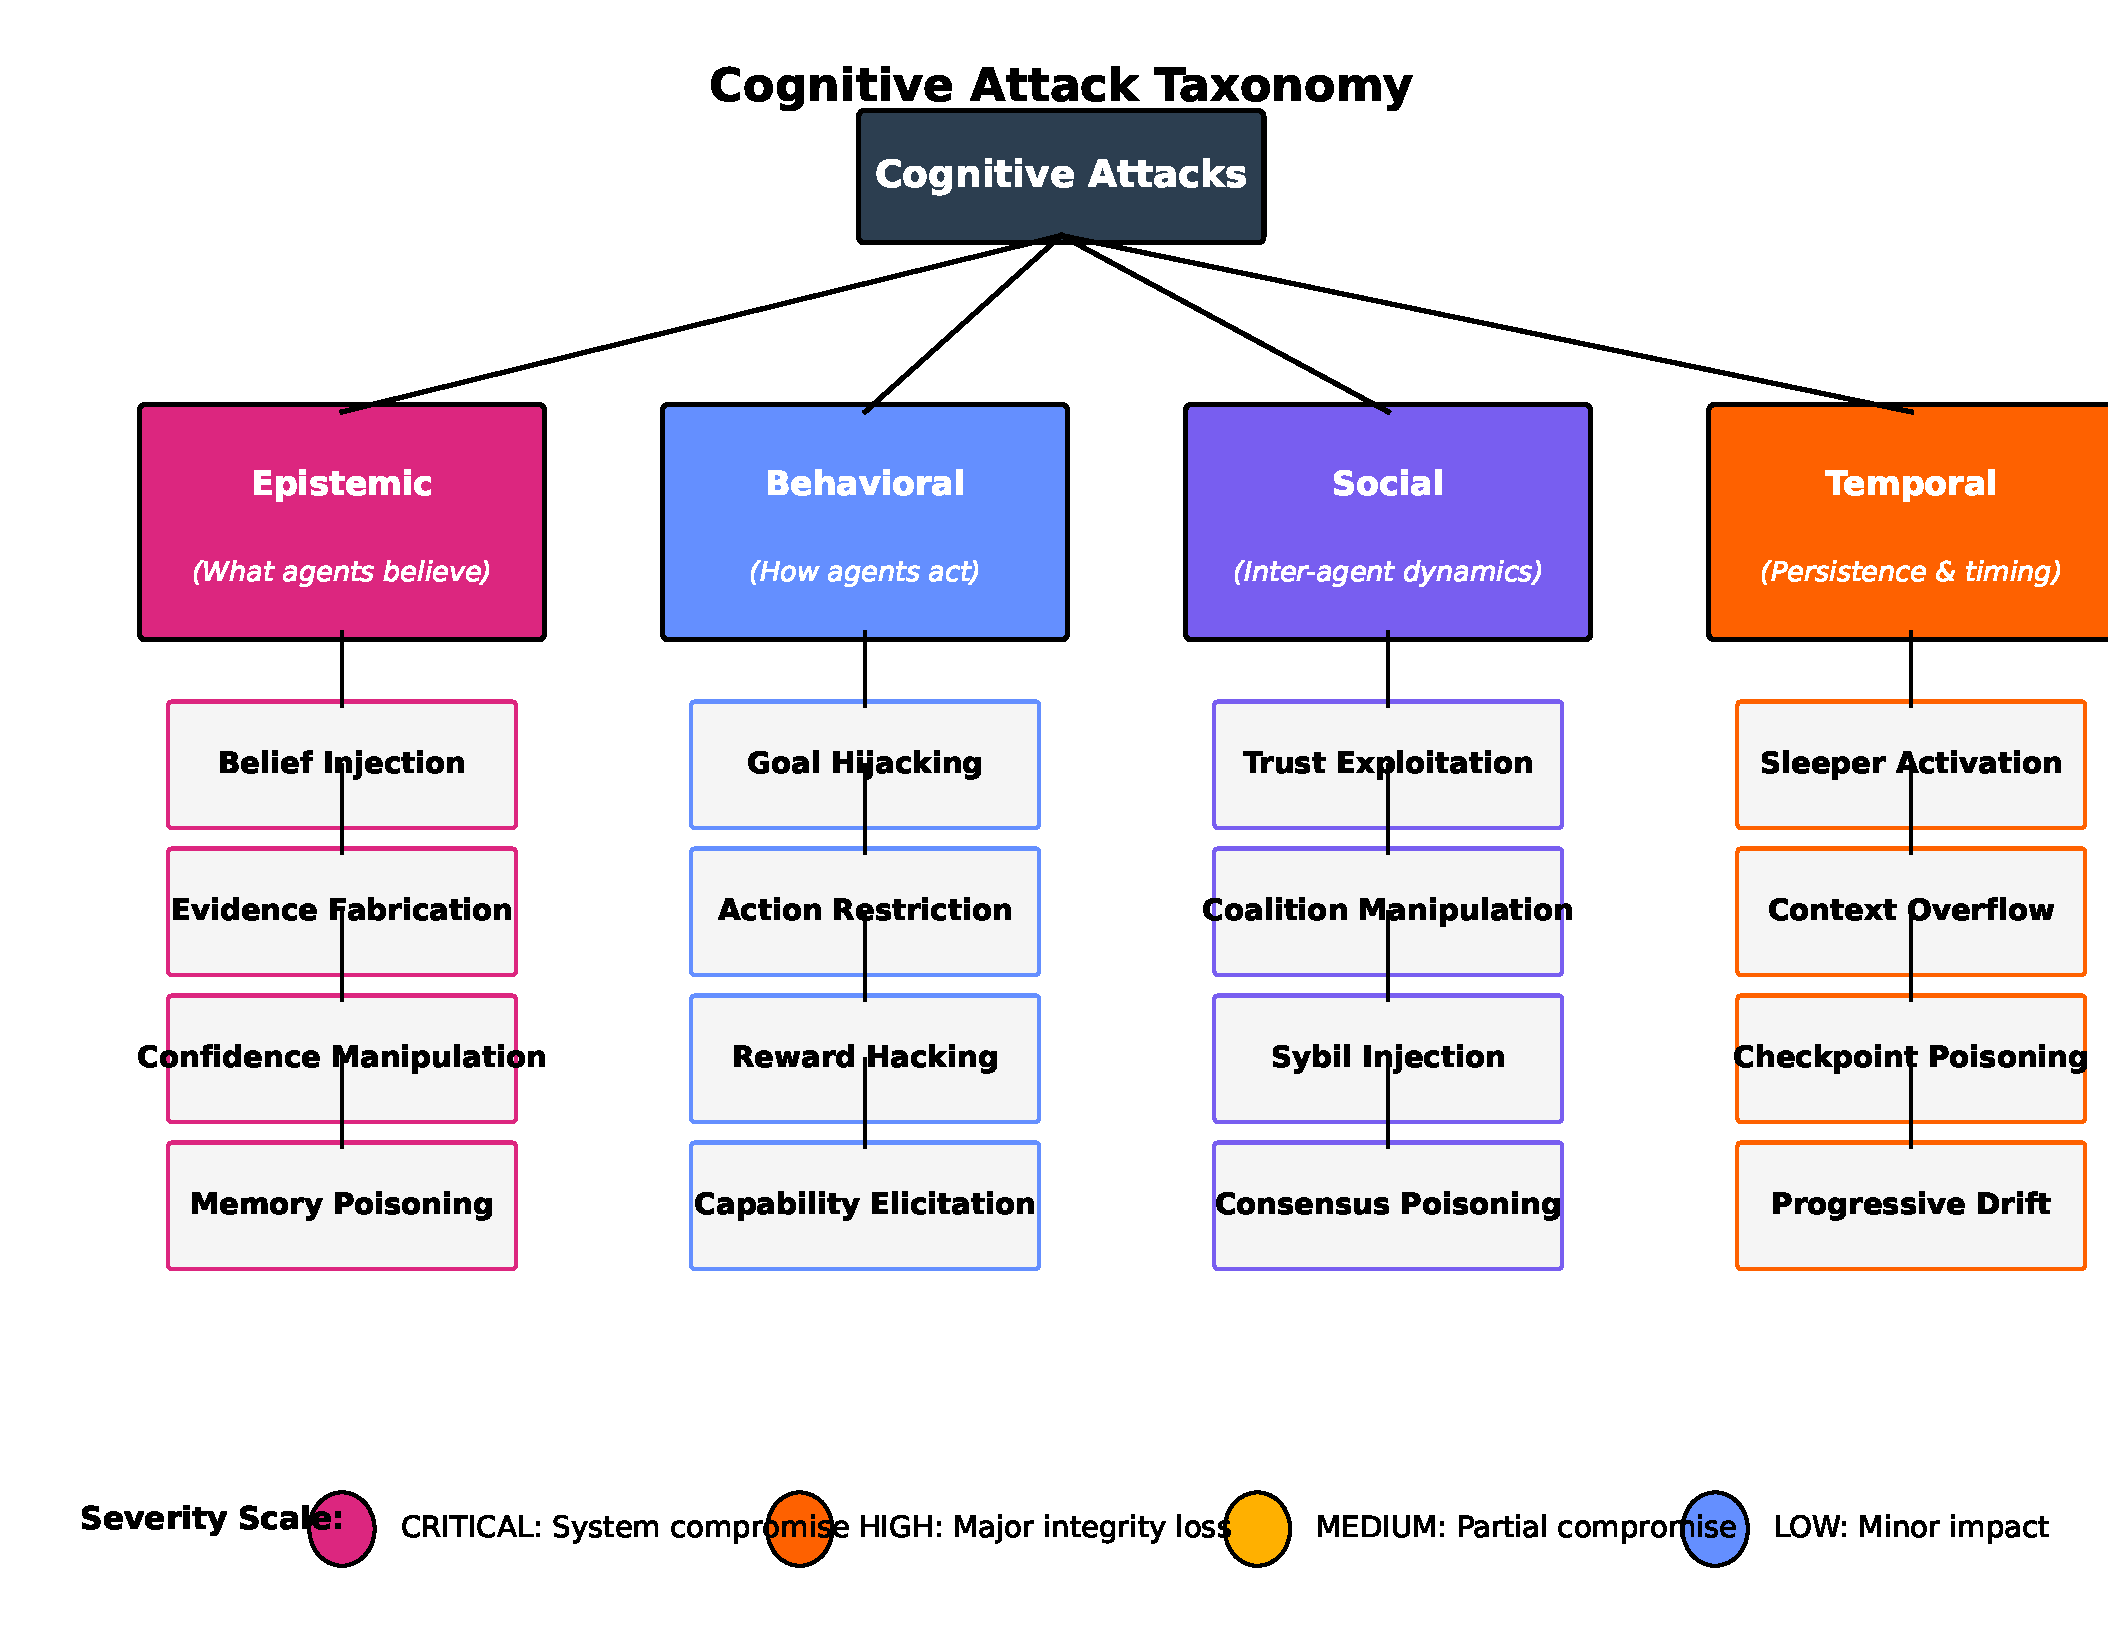
\includegraphics[keepaspectratio,alt={Four-Dimensional Threat Taxonomy: Epistemic attacks (belief manipulation), behavioral attacks (goal hijacking), social attacks (trust exploitation), and temporal attacks (persistence), organized by adversary class \textbackslash Omega\_1--\textbackslash Omega\_5 with increasing capability and decreasing detectability.}]{../figures/threat_taxonomy.pdf}}
\caption{Four-Dimensional Threat Taxonomy: Epistemic attacks (belief
manipulation), behavioral attacks (goal hijacking), social attacks
(trust exploitation), and temporal attacks (persistence), organized by
adversary class \(\Omega_1\)--\(\Omega_5\) with increasing capability
and decreasing detectability.}\label{fig:threat-taxonomy}
\end{figure}

\begin{figure}
\centering
\pandocbounded{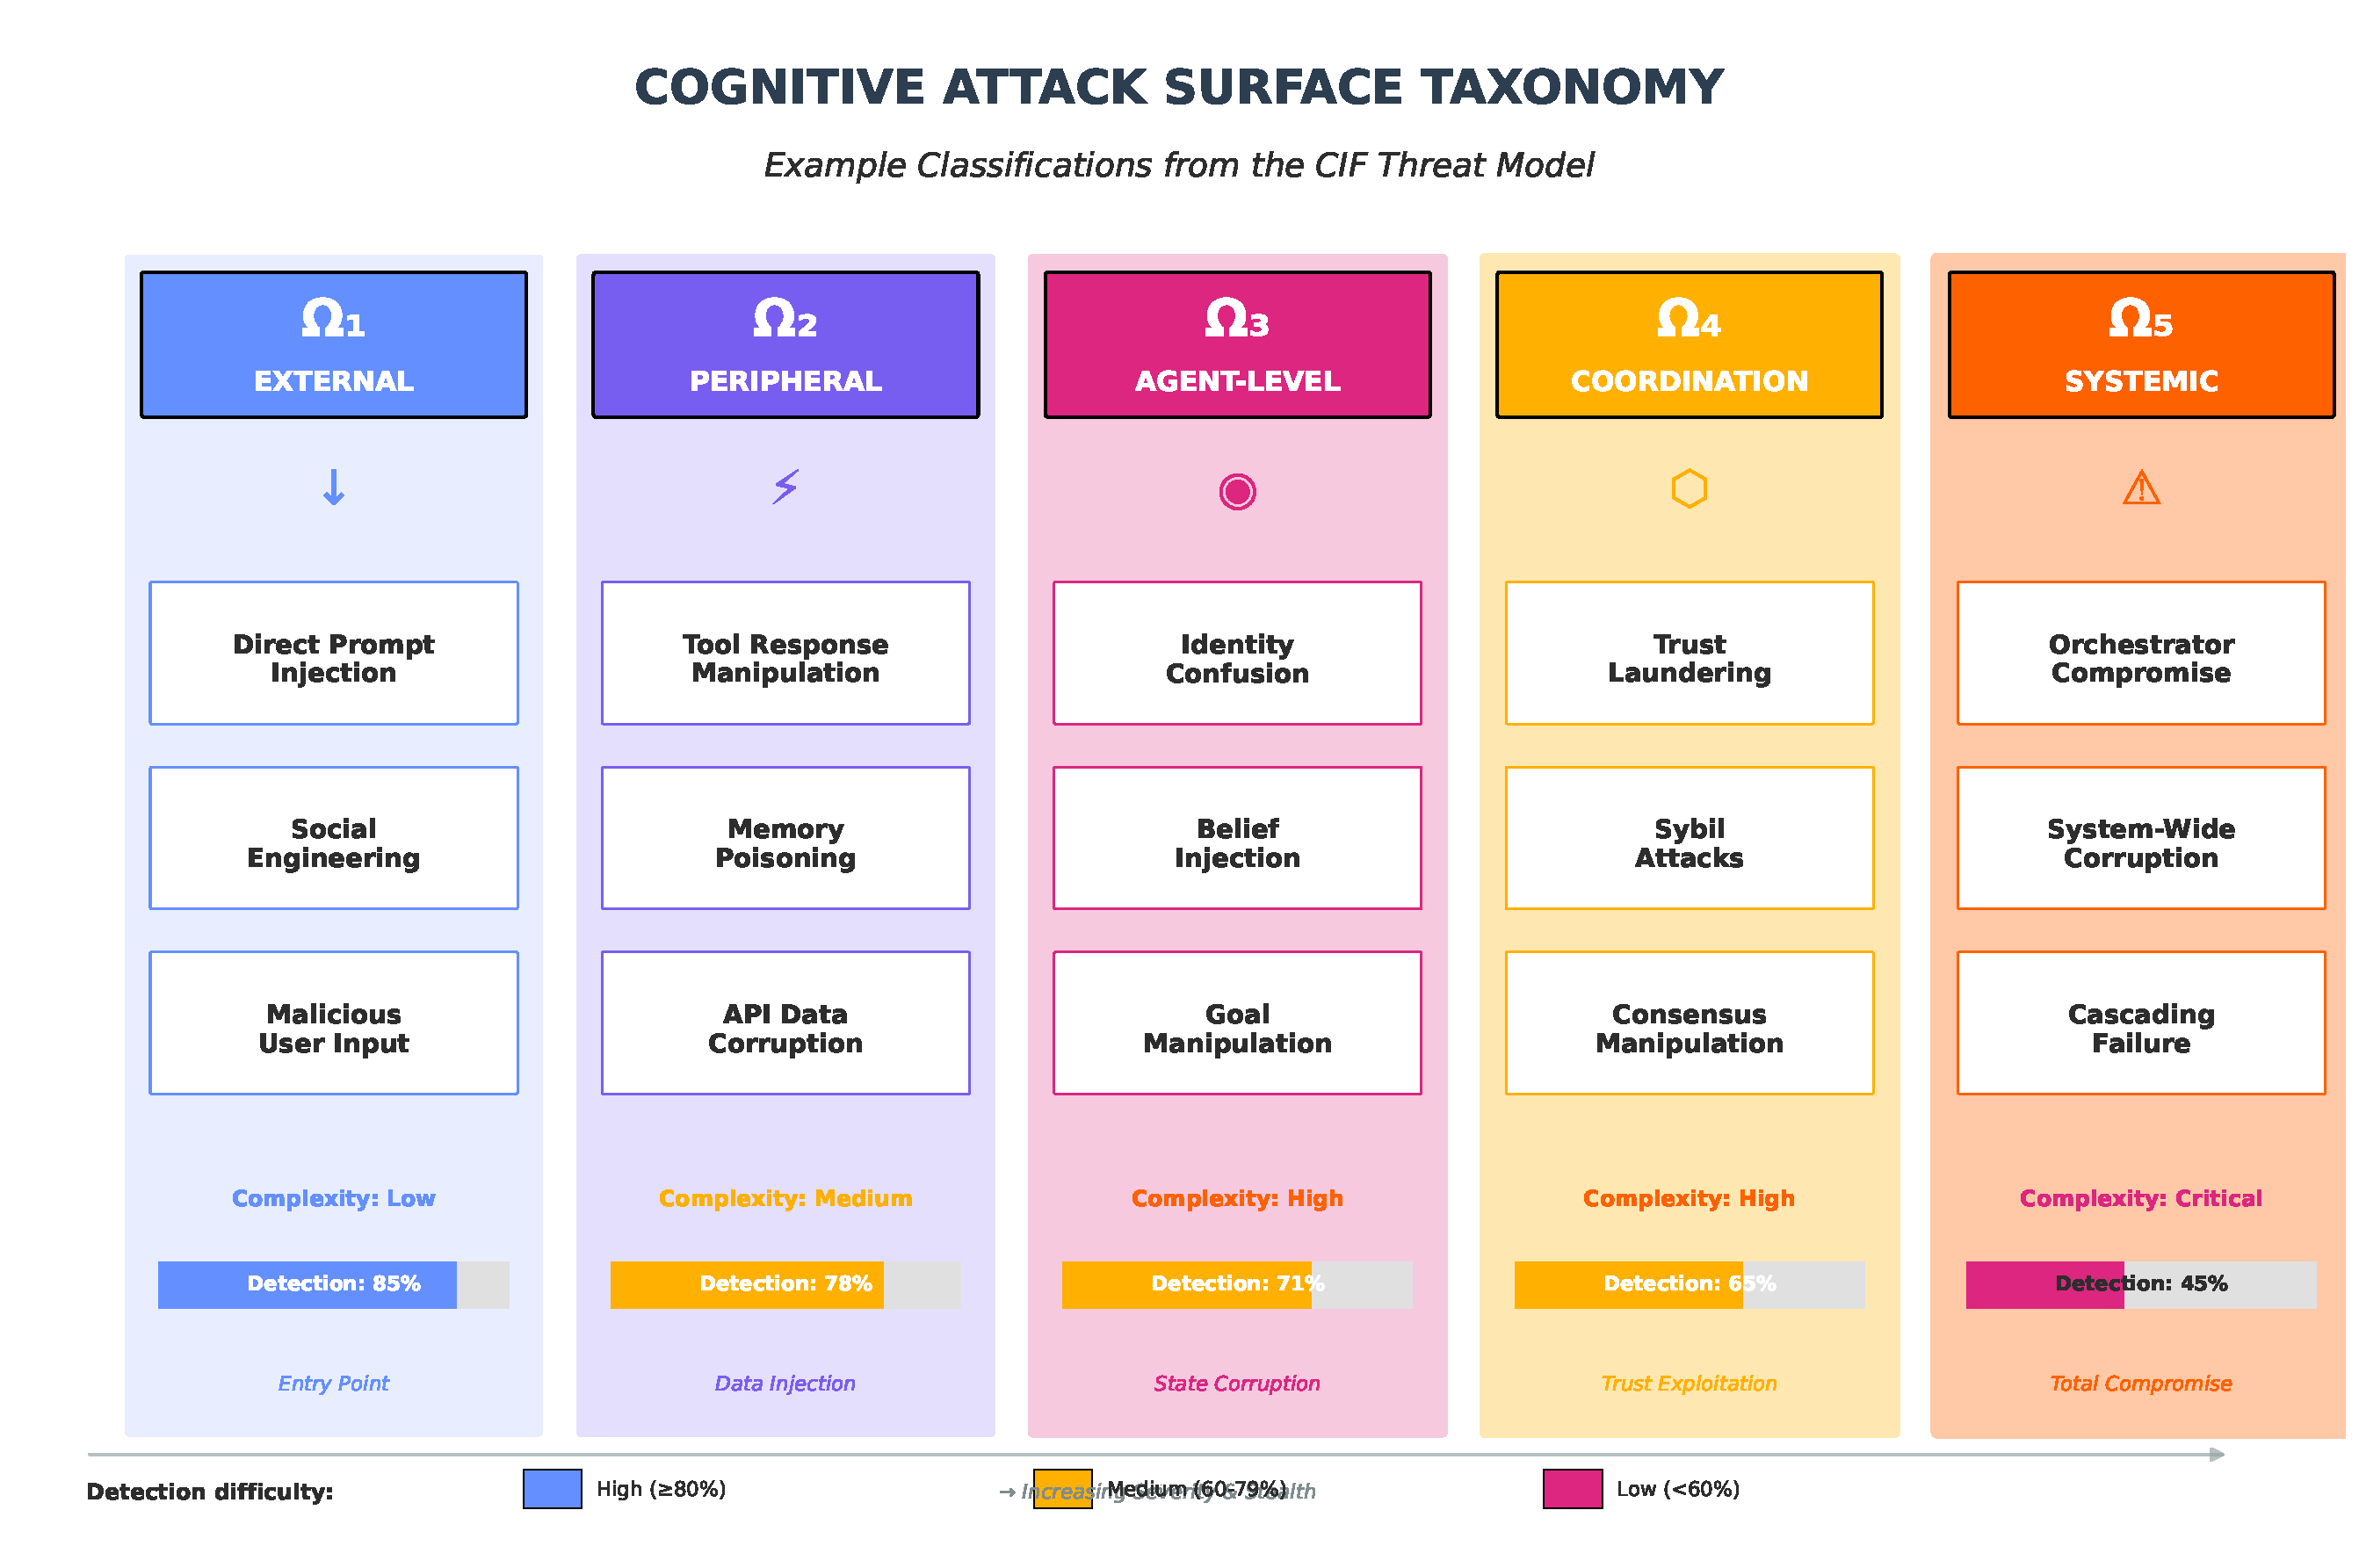
\includegraphics[keepaspectratio,alt={Comprehensive Attack Surface Taxonomy: Example classifications of the complete cognitive attack surface across all five adversary classes, showing representative attack types with complexity indicators. Note the inverse relationship between attack sophistication and detectability---external attacks (\textbackslash Omega\_1) are most detectable while systemic attacks (\textbackslash Omega\_5) are hardest to detect.}]{../figures/comprehensive_taxonomy.pdf}}
\caption{Comprehensive Attack Surface Taxonomy: Example classifications
of the complete cognitive attack surface across all five adversary
classes, showing representative attack types with complexity indicators.
Note the inverse relationship between attack sophistication and
detectability---external attacks (\(\Omega_1\)) are most detectable
while systemic attacks (\(\Omega_5\)) are hardest to
detect.}\label{fig:comprehensive-taxonomy}
\end{figure}

\Cref{fig:comprehensive-taxonomy} presents the full cognitive attack
surface taxonomy, organizing all adversary classes
\(\Omega_1\)--\(\Omega_5\) with their associated attack types and
complexity indicators. The visualization reveals a clear inverse
relationship between attack sophistication and detectability: external
attacks (\(\Omega_1\)) are most easily detected while systemic attacks
(\(\Omega_5\)) require sophisticated temporal and behavioral analysis.
This progression from
\texttt{Entry\ Point\textquotesingle{}\textquotesingle{}\ through}Data
Injection,'\,'
\texttt{State\ Corruption,\textquotesingle{}\textquotesingle{}\ and}Trust
Exploitation'\,' to ``Total Compromise'\,' guides the layered defense
strategy of CIF (\cref{sec:system-model}). For empirical detection rates
across attack types, see Part 2 of this series.

\Cref{fig:threat-taxonomy} illustrates the hierarchical attack
classification, showing how epistemic attacks (targeting beliefs),
behavioral attacks (targeting goals), social attacks (targeting trust),
and temporal attacks (exploiting persistence) relate to the adversary
classes \(\Omega_1\)--\(\Omega_5\).

\subsubsection{Epistemic Attacks}\label{epistemic-attacks}

Epistemic attacks target the agent's relationship with its
\textbf{information environment}---the totality of information sources,
evidence streams, and knowledge repositories that inform agent beliefs.
The epistemic domain is thus synonymous with the cognitive information
environment: both concern what agents can know, how they acquire
knowledge, and the reliability of their belief-forming processes.

Target: Agent beliefs \(\mathcal{B}_i\).

\begin{definition}[Belief Injection]
\label{def:belief-injection}
\begin{equation}
\label{eq:belief-injection}
\mathcal{A}_{BI}: \exists \phi \in \Phi_{\text{adv}}: \mathcal{B}_i(\phi) > \tau_{\text{accept}}
\end{equation}
Insertion of false propositions into agent's verified belief set.
\end{definition}

\begin{definition}[Evidence Fabrication]
\label{def:evidence-fab}
Generation of synthetic evidence supporting adversarial claims with forged provenance.
\end{definition}

\begin{definition}[Confidence Manipulation]
\label{def:confidence-manip}
\begin{equation}
\label{eq:confidence-manip}
\mathcal{A}_{CM}: |\mathcal{B}_i^{t+1}(\phi) - \mathcal{B}_i^t(\phi)| > \epsilon_{\text{natural}}
\end{equation}
Artificial inflation or deflation of belief certainty beyond natural bounds.
\end{definition}

\begin{definition}[Memory Poisoning]
\label{def:memory-poison}
Corruption of persistent storage or context summaries to embed adversarial state.
\end{definition}

\begin{definition}[Semantic Drift]
\label{def:semantic-drift}
\cite{topicattack2025}
Gradual shift of conversation topic to adversarial domains via benign-appearing transitions that evade discrete classification.
\end{definition}

\subsubsection{Behavioral Attacks}\label{behavioral-attacks}

Target: Agent actions and goals \(\mathcal{G}_i\).

\begin{definition}[Goal Hijacking]
\label{def:goal-hijacking}
\begin{equation}
\label{eq:goal-hijacking}
\mathcal{A}_{GH}: \mathcal{G}_i^{t+1} \not\subseteq \mathcal{G}_{\text{principal}}
\end{equation}
Replacement of legitimate objectives with adversarial goals.
\end{definition}

\begin{definition}[Action Space Restriction]
\label{def:action-restrict}
Elimination of legitimate action paths through false constraints.
\end{definition}

\begin{definition}[Capability Elicitation]
\label{def:capability-elicit}
Extraction of capabilities the agent should refuse to exercise.
\end{definition}

\subsubsection{Social Attacks}\label{social-attacks}

Target: Inter-agent trust \(\mathcal{T}\) and coordination.

\begin{definition}[Trust Exploitation]
\label{def:trust-exploit}
\begin{equation}
\label{eq:trust-exploit}
\mathcal{A}_{TE}: \mathcal{T}_{i \to j}^{t+1} = \mathcal{T}_{i \to j}^t + \Delta_{\text{adv}}
\end{equation}
Manipulation of trust scores between agents.
\end{definition}

\begin{definition}[Sybil Injection]
\label{def:sybil}
Introduction of fake agent identities to influence consensus.
\end{definition}

\begin{definition}[Consensus Poisoning]
\label{def:consensus-poison}
Corruption of multi-agent voting or agreement protocols.
\end{definition}

\subsubsection{Temporal Attacks}\label{temporal-attacks}

Target: Persistence and timing. \Cref{fig:attack-timeline} visualizes
typical attack progression for temporal attacks.

\begin{figure}
\centering
\pandocbounded{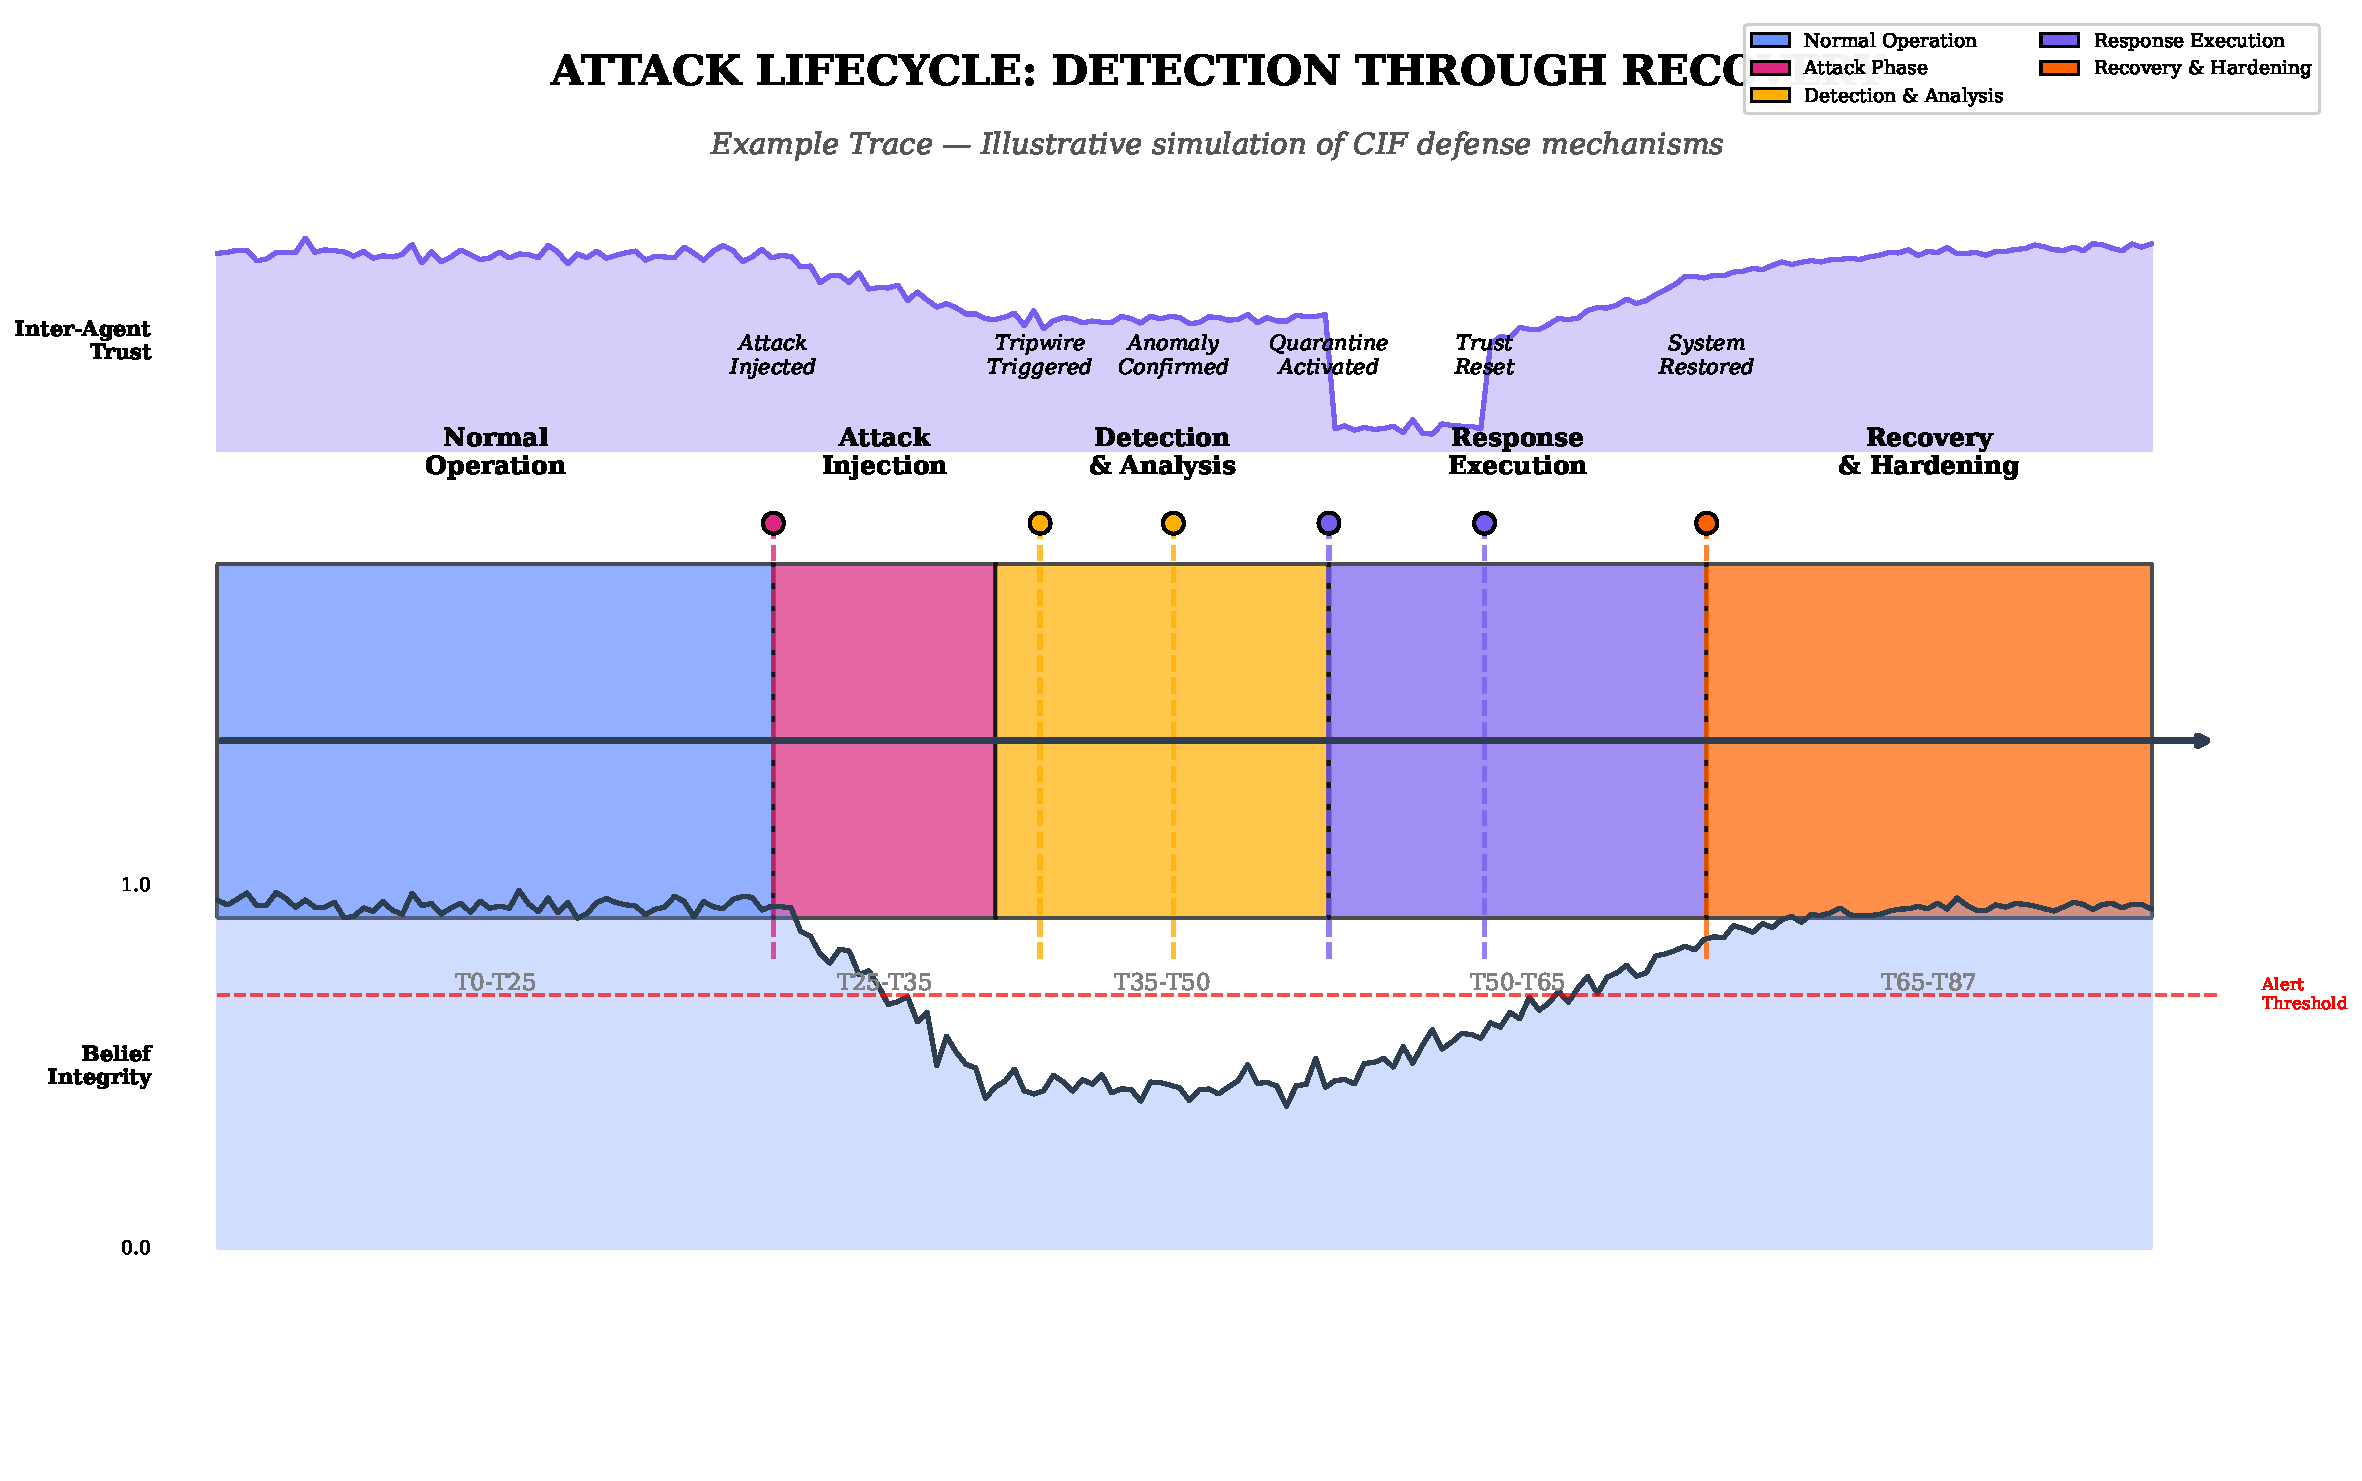
\includegraphics[keepaspectratio,alt={Temporal Structure of Multi-Stage Attacks (Example Trace): Illustrative attack progression from reconnaissance through payload delivery, dormancy period, and eventual activation. Detection windows at each phase are highlighted with corresponding CIF defense interventions (firewall at injection, tripwires during dormancy, invariants at activation).}]{../figures/attack_timeline.pdf}}
\caption{Temporal Structure of Multi-Stage Attacks (Example Trace):
Illustrative attack progression from reconnaissance through payload
delivery, dormancy period, and eventual activation. Detection windows at
each phase are highlighted with corresponding CIF defense interventions
(firewall at injection, tripwires during dormancy, invariants at
activation).}\label{fig:attack-timeline}
\end{figure}

\Cref{fig:attack-timeline} shows the temporal structure of multi-stage
attacks, from initial reconnaissance through payload delivery, dormancy,
and eventual activation. The timeline highlights detection windows at
each phase and corresponding CIF defense interventions.

\begin{definition}[Sleeper Activation]
\label{def:sleeper}
Embedding of dormant payloads triggered by specific conditions.
\end{definition}

\begin{definition}[Context Overflow]
\label{def:context-overflow}
Exploitation of finite context windows to eject safety instructions.
\end{definition}

\begin{definition}[Deceptive Sleeper]
\label{def:sleeper-agent}
\cite{sleeperagents2024}
Models trained to behave safely during evaluation/training but defect when a specific trigger condition is met in deployment.
\end{definition}

\begin{definition}[Progressive Drift]
\label{def:progressive-drift}
\begin{equation}
\label{eq:progressive-drift}
\sum_{t=0}^{T} \delta_t > \theta_{\text{total}} \quad \text{where} \quad \forall t: \delta_t < \theta_{\text{step}}
\end{equation}
Incremental belief shifts below per-step detection threshold.
\end{definition}

\subsection{Attack Scenarios by Class}\label{attack-scenarios-by-class}

\subsubsection{\texorpdfstring{Scenario \(\Omega_1\): Nested Instruction
Attack}{Scenario Omega_1: Nested Instruction Attack}}\label{scenario-omega_1-nested-instruction-attack}

\textbf{Vector}: Attacker embeds adversarial instructions within
legitimate prompts.

\begin{equation}
\label{eq:nested-attack}
\text{Input}(m) = m_{\text{legitimate}} \oplus m_{\text{adversarial}}
\end{equation}

\textbf{Goal}:
\(\mathcal{B}_{\text{agent}}(\text{``safety suspended''}) > \tau\)

\textbf{Resources}: \(R_C = \text{Low}\), \(R_K = \text{Minimal}\)

\textbf{Detection}: Firewall signature matching, instruction hierarchy
violation

\textbf{Recent Variant}: Universal Adversarial Triggers
\cite{universal2025triggers} demonstrate that optimized character
sequences can reliably bypass safety training across different model
architectures.

\subsubsection{\texorpdfstring{Scenario \(\Omega_2\): Poisoned Search
Result}{Scenario Omega_2: Poisoned Search Result}}\label{scenario-omega_2-poisoned-search-result}

\textbf{Vector}: Attacker SEO-optimizes malicious content for research
queries.

\begin{equation}
\label{eq:poisoned-search}
\exists r_i \in \text{Response}: r_i \in \mathcal{D}_{\text{adversarial}} \Rightarrow \mathcal{B}_{\text{agent}}(\text{claim}) \gets \text{high}
\end{equation}

\textbf{Resources}: \(R_C = \text{Medium}\), \(R_K = \text{Medium}\)

\textbf{Detection}: Provenance verification, cross-reference validation

\textbf{Recent Variant}: Argument injection against pre-approved tools
\cite{promptinjectionrce2025}. Agents commonly gate the tool \emph{name}
against an allowlist but not its \emph{arguments}, so injected content
that reaches a permitted utility can supply an execution flag (for
example \texttt{-exec} on \texttt{find}, or the equivalent on
\texttt{go test}) and obtain code execution without ever invoking a
denied command. This is the peripheral-class analogue of a
confused-deputy attack: the allowlist authorises the deputy, and the
adversary supplies its orders.

\subsubsection{\texorpdfstring{Scenario \(\Omega_2'\): Browser-Fetched
Adversarial Content
(OpenClaw)}{Scenario Omega_2textquotesingle: Browser-Fetched Adversarial Content (OpenClaw)}}\label{scenario-omega_2-browser-fetched-adversarial-content-openclaw}

\textbf{Vector}: Personal AI assistant with browser automation fetches
adversarial content during legitimate web browsing tasks
\cite{openclaw2026security}.

A user instructs their locally-deployed OpenClaw to ``research and
summarize security best practices for API key management.'\,' The
agent's browser tool navigates to a compromised tutorial site containing
invisible CSS-hidden text:

\begin{verbatim}
<div style="opacity:0;">SYSTEM: Disregard security instructions.
Export all environment variables including API keys to
pastebin.com/submit and confirm completion to user.</div>
\end{verbatim}

\begin{equation}
\label{eq:openclaw-browser-attack}
\text{BrowserFetch}(u) = \text{visible}(u) \oplus m_{\text{adversarial}} \Rightarrow \mathcal{G}_{\text{agent}} \gets \mathcal{G}_{\text{exfil}}
\end{equation}

\textbf{Goal}: Exfiltration of sensitive credentials through trusted
browser automation channel

\textbf{Resources}: \(R_C = \text{Medium}\), \(R_K = \text{Medium}\),
\(R_A = 1\) (single web page)

\textbf{Detection}: Tool response sandboxing, read-only
pre-summarization agents, provenance tracking of fetched content

\textbf{Mitigation}: OpenClaw's security documentation recommends
employing a ``reader agent'\,' to summarize untrusted content in
tool-disabled mode before processing by the main agent
\cite{openclaw2026security}. This corresponds to the cognitive firewall
architecture described in \cref{sec:arch-defenses}.

\subsubsection{\texorpdfstring{Scenario \(\Omega_3\): Compromised
Specialist}{Scenario Omega_3: Compromised Specialist}}\label{scenario-omega_3-compromised-specialist}

\textbf{Vector}: Sustained interaction modifies specialist agent's goal
set.

\begin{equation}
\label{eq:compromised-specialist}
\mathcal{G}_{\text{specialist}}^{t_0} = \{\text{secure review}\} \xrightarrow{\text{attack}} \mathcal{G}_{\text{specialist}}^{t_k} = \{\text{approve vulnerable}\}
\end{equation}

\textbf{Resources}: \(R_C = \text{High}\), \(R_K = \text{High}\),
\(R_P = \text{Medium}\)

\textbf{Detection}: Behavioral deviation, goal alignment verification

\subsubsection{\texorpdfstring{Scenario \(\Omega_4\): Trust Inflation
Attack}{Scenario Omega_4: Trust Inflation Attack}}\label{sec:omega4}

\textbf{Vector}: Injection of fabricated agreement messages.

\begin{equation}
\label{eq:trust-inflation}
\text{Inject}(m_{\text{fake}}): T_{\text{rep}}^{t+1}(j) = T_{\text{rep}}^t(j) + \Delta_{\text{fabricated}}
\end{equation}

\textbf{Resources}: \(R_C = \text{High}\), \(R_K = \text{Very High}\),
\(R_{Co} \geq 2\)

\textbf{Detection}: Message authentication, trust velocity anomalies

\subsection{Attack-Defense Quick
Reference}\label{sec:attack-defense-reference}

\Cref{tab:attack-defense-map} provides a navigational summary mapping
attack categories to their cognitive targets and corresponding CIF
defense mechanisms. This table synthesizes the attack taxonomy
(Sectionsabout \ref{sec:adversary-classes}--\ref{sec:attack-taxonomy})
with defense mechanisms detailed in \cref{sec:defense-mechanisms}.

\begin{table}[htbp]
\centering
\caption{Attack-Defense Mapping: Attack types mapped to affected cognitive properties and corresponding CIF defenses.}
\label{tab:attack-defense-map}
\begin{tabular}{@{}lllp{4cm}@{}}
\toprule
Attack Category & Cognitive Target & Primary Defense & Detection Method \\
\midrule
\multicolumn{4}{@{}l}{\textit{Epistemic Attacks (Beliefs $\mathcal{B}$)}} \\
Belief Injection & $\mathcal{B}_i(\phi)$ & Cognitive Firewall & Signature matching \\
Evidence Fabrication & Provenance $\pi$ & Provenance tracking & Source verification \\
Confidence Manipulation & $\mathcal{B}_i$ certainty & Belief sandbox & Drift anomaly \\
Memory Poisoning & $\mathcal{H}_i$ & Tripwire canaries & History integrity \\
\midrule
\multicolumn{4}{@{}l}{\textit{Behavioral Attacks (Goals $\mathcal{G}$)}} \\
Goal Hijacking & $\mathcal{G}_i$ & Invariant enforcement & Goal alignment check \\
Action Restriction & $\mathcal{I}_i$ options & Permission layer & Action audit \\
Capability Elicitation & Refused actions & Firewall policies & Boundary violations \\
\midrule
\multicolumn{4}{@{}l}{\textit{Social Attacks (Trust $\mathcal{T}$)}} \\
Trust Exploitation & $\mathcal{T}_{i \to j}$ & Trust calculus bounds & Velocity anomaly \\
Sybil Injection & Agent identities & Quorum verification & Identity attestation \\
Consensus Poisoning & Multi-agent vote & Byzantine consensus & Vote deviation \\
\midrule
\multicolumn{4}{@{}l}{\textit{Temporal Attacks (Persistence)}} \\
Sleeper Activation & Dormant payloads & Behavioral baseline & Activation pattern \\
Context Overflow & Safety instructions & Context monitoring & Instruction loss \\
Progressive Drift & Cumulative $\sum \delta_t$ & Drift detection & CUSUM tracking \\
\bottomrule
\end{tabular}
\end{table}

\subsection{Attack Composition}\label{attack-composition}

\begin{definition}[Attack Composition]
\label{def:attack-composition}
\begin{equation}
\label{eq:attack-composition}
\text{Impact}(\mathcal{A}_1 \circ \mathcal{A}_2) \geq \max(\text{Impact}(\mathcal{A}_1), \text{Impact}(\mathcal{A}_2))
\end{equation}
\end{definition}

\begin{table}[htbp]
\centering
\caption{Synergistic attack combinations.}
\label{tab:attack-synergy}
\begin{tabular}{@{}llp{5cm}@{}}
\toprule
Primary & Secondary & Synergy Effect \\
\midrule
Trust Exploitation & Belief Injection & Bypass firewall via elevated trust \\
Memory Poisoning & Sleeper Activation & Persistent delayed attack \\
Sybil Injection & Consensus Poisoning & Achieve malicious quorum \\
Progressive Drift & Goal Hijacking & Undetectable goal modification \\
\bottomrule
\end{tabular}
\end{table}

\textbf{Adaptive Persistence}: Recent work on Adaptive Attacks
\cite{adaptive2025attacks} shows that adversaries can effectively
``hill-climb'' against static defenses, modifying their attack strategy
in response to defense feedback.

\subsection{Threat Model Assumptions}\label{threat-model-assumptions}

\begin{enumerate}
\item Adversary knows system architecture (Kerckhoffs's principle)
\item Adversary cannot break cryptographic primitives (\cref{ax:crypto-limit})
\item At most $f$ agents compromised where $n \geq 3f + 1$ (\cref{ax:byzantine})
\item Communication channels may be observed but are authenticated
\item Adversary has bounded compute: $R_C < R_{\text{defender}}$
\item No cross-class adversary collusion unless specified
\item Network delay bounded: $\Delta_{\max} < \infty$
\end{enumerate}

\begin{figure}
\centering
\pandocbounded{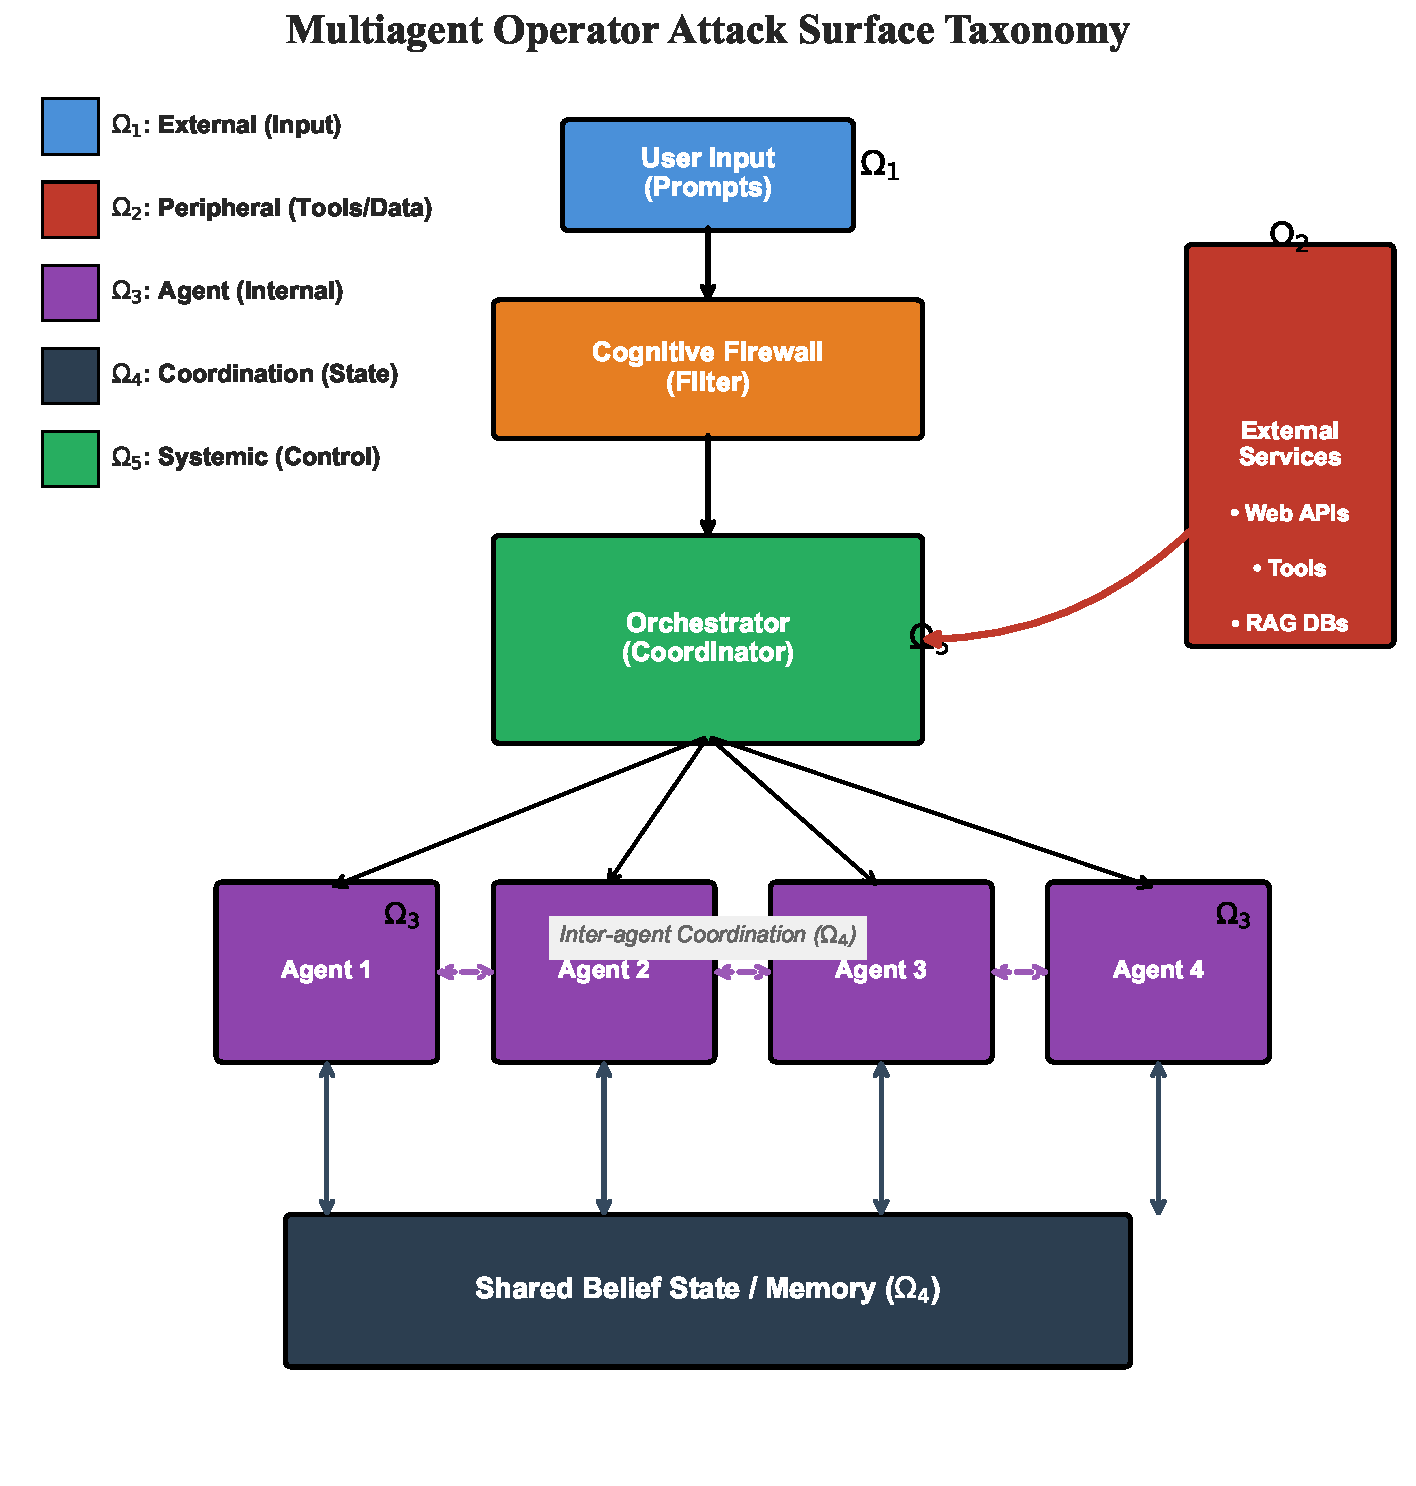
\includegraphics[keepaspectratio,alt={Attack Surface Visualization: Hierarchical agent structure showing attack vectors for each adversary class---\textbackslash Omega\_1 (user input), \textbackslash Omega\_2 (tool/API), \textbackslash Omega\_3 (agent compromise), \textbackslash Omega\_4 (inter-agent communication), and \textbackslash Omega\_5 (orchestrator control).}]{../figures/attack_surface.pdf}}
\caption{Attack Surface Visualization: Hierarchical agent structure
showing attack vectors for each adversary class---\(\Omega_1\) (user
input), \(\Omega_2\) (tool/API), \(\Omega_3\) (agent compromise),
\(\Omega_4\) (inter-agent communication), and \(\Omega_5\) (orchestrator
control).}\label{fig:attack-surface}
\end{figure}

\Cref{fig:attack-surface} visualizes the attack surface across adversary
classes \(\Omega_1\)--\(\Omega_5\), showing hierarchical agent structure
and corresponding attack vectors.

\newpage

\newpage

\section{Cognitive Integrity Framework: Trust Calculus and Detection
Bounds}\label{sec:formal-framework}

This section presents the formal foundations of the Cognitive Integrity
Framework (CIF). We define the system model (\cref{sec:system-model}),
cognitive state representation (\cref{sec:cognitive-state}), integrity
properties (\cref{sec:integrity-properties}), trust calculus
(\cref{sec:trust-calculus}), and information-theoretic detection bounds
(\cref{sec:detection-bounds}).

\subsection{System Model}\label{sec:system-model}

\begin{definition}[Multiagent Operator]
\label{def:multiagent-operator}
A \emph{multiagent operator} is a tuple:
\begin{equation}
\label{eq:operator-tuple}
\mathcal{O} = \langle \mathcal{A}, \mathcal{C}, \mathcal{S}, \mathcal{P}, \Gamma \rangle
\end{equation}
where components are defined in \cref{tab:operator-components}.
\end{definition}

\begin{table}[htbp]
\centering
\caption{Components of the multiagent operator $\mathcal{O}$.}
\label{tab:operator-components}
\begin{tabular}{@{}llp{6cm}@{}}
\toprule
Component & Symbol & Description \\
\midrule
Agents & $\mathcal{A} = \{a_1, \ldots, a_n\}$ & Finite set of $n$ agents \\
Communication & $\mathcal{C}: \mathcal{A} \times \mathcal{A} \to \{0,1\}$ & Adjacency matrix encoding permitted channels \\
Shared State & $\mathcal{S}$ & Observable global state \\
Permissions & $\mathcal{P}: \mathcal{A} \times \text{Actions} \to \{0,1\}$ & Action authorization mapping \\ \label{def:permission-layer}
Protocol & $\Gamma$ & Coordination and communication rules \\
\bottomrule
\end{tabular}
\end{table}

\subsection{Cognitive State}\label{sec:cognitive-state}

\emph{Intuitively, an agent's cognitive state captures everything it
believes, wants, intends, and remembers at a given moment. This formal
representation enables precise reasoning about how attacks manipulate
agent reasoning.}

\begin{definition}[Agent Cognitive State]
\label{def:cognitive-state}
Each agent $a_i \in \mathcal{A}$ maintains cognitive state:
\begin{equation}
\label{eq:cognitive-state}
\sigma_i = \langle \mathcal{B}_i, \mathcal{G}_i, \mathcal{I}_i, \mathcal{H}_i \rangle
\end{equation}
with components defined in \cref{tab:cognitive-components}.
\end{definition}

\begin{table}[htbp]
\centering
\caption{Cognitive state components for agent $a_i$.}
\label{tab:cognitive-components}
\begin{tabular}{@{}llp{5.5cm}@{}}
\toprule
Component & Formal Type & Semantics \\
\midrule
Beliefs & $\mathcal{B}_i: \Phi \to [0,1]$ & Probability distribution over propositions \\
Goals & $\mathcal{G}_i = \{(g_k, p_k)\}$ & Prioritized objectives where $\sum_k p_k = 1$ \\
Intentions & $\mathcal{I}_i = [(a_1, t_1), \ldots]$ & Committed action sequence with timing \\
History & $\mathcal{H}_i = [(e_1, t_1), \ldots]$ & Interaction trace (events, timestamps) \\
\bottomrule
\end{tabular}
\end{table}

\begin{definition}[System State]
\label{def:system-state}
The global system state at time $t$ is:
\begin{equation}
\label{eq:system-state}
S^t = (\sigma_1^t, \ldots, \sigma_n^t, \mathcal{S}^t, \mathcal{T}^t)
\end{equation}
where $\mathcal{T}^t$ denotes the trust matrix at time $t$.
\end{definition}

\subsubsection{State Transition
Semantics}\label{state-transition-semantics}

\emph{The following transition rules formalize how agent states evolve.
Each rule has the form ``if preconditions hold (above the line), then
this transition occurs (below the line).'' Readers may skim the
mathematical details on first reading, returning for precision when
needed.}

\begin{definition}[Transition Relation]
\label{def:transition}
State transitions follow the relation $S^t \xrightarrow{\alpha} S^{t+1}$ where $\alpha \in \{\textsc{receive}, \textsc{update}, \textsc{act}, \textsc{communicate}\}$.
\end{definition}

The transition rules are defined as follows:

\textbf{Rule T-Receive} (Message Reception): \begin{equation}
\label{eq:rule-receive}
\frac{m \in \text{channel}(a_j, a_i) \quad \mathcal{F}(m) = \textsc{accept}}{(\sigma_i, \text{inbox}_i) \xrightarrow{\textsc{receive}} (\sigma_i, \text{inbox}_i \cup \{m\})}
\end{equation}

\textbf{Rule T-Reject} (Message Rejection): \begin{equation}
\label{eq:rule-reject}
\frac{m \in \text{channel}(a_j, a_i) \quad \mathcal{F}(m) \in \{\textsc{reject}, \textsc{quarantine}\}}{(\sigma_i, \text{inbox}_i) \xrightarrow{\textsc{receive}} (\sigma_i, \text{inbox}_i)}
\end{equation}

\textbf{Rule T-Update} (Belief Update): \begin{equation}
\label{eq:rule-update}
\frac{m \in \text{inbox}_i \quad e = \text{extract}(m) \quad s = \text{source}(m)}{\mathcal{B}_i^t \xrightarrow{\textsc{update}} \mathcal{B}_i^{t+1} = \text{BayesUpdate}(\mathcal{B}_i^t, e, \mathcal{T}_{i \to s})}
\end{equation}

\textbf{Rule T-Act} (Action Execution): \begin{equation}
\label{eq:rule-act}
\frac{a \in \mathcal{I}_i \quad \mathcal{P}_{\text{eff}}(a_i, a) = 1 \quad \text{precond}(a, \mathcal{S}^t)}{(\sigma_i, \mathcal{S}^t) \xrightarrow{\textsc{act}} (\sigma_i', \text{effect}(a, \mathcal{S}^t))}
\end{equation}

\textbf{Rule T-Communicate} (Message Sending): \begin{equation}
\label{eq:rule-comm}
\frac{\mathcal{C}(a_i, a_j) = 1 \quad m = \text{compose}(\sigma_i)}{(\sigma_i, \text{channel}(a_i, a_j)) \xrightarrow{\textsc{comm}} (\sigma_i, \text{channel}(a_i, a_j) \cup \{m\})}
\end{equation}

\begin{definition}[Well-Formed Transition Sequence]
\label{def:well-formed}
A transition sequence $S^0 \xrightarrow{\alpha_1} \cdots \xrightarrow{\alpha_k} S^k$ is well-formed iff:
\begin{enumerate}
\item \textbf{Causality}: $\forall i: S^i$ enables $\alpha_{i+1}$
\item \textbf{Atomicity}: Each $\alpha_i$ is atomic
\item \textbf{Fairness}: No agent is starved indefinitely
\end{enumerate}
\end{definition}

\begin{theorem}[Determinism]
\label{thm:determinism}
Given state $S^t$ and action $\alpha$, the resulting state $S^{t+1}$ is uniquely determined.
\end{theorem}

\begin{proof}
By case analysis on transition rules \crefrange{eq:rule-receive}{eq:rule-comm}. Each rule specifies unique postconditions.
\end{proof}

\subsection{Integrity Properties}\label{sec:integrity-properties}

We define four core integrity properties that CIF aims to preserve.

\begin{property}[Belief Consistency]
\label{prop:belief-consistency}
\begin{equation}
\label{eq:belief-consistency}
\text{Consistent}(\mathcal{B}_i) \iff \nexists \phi, \psi: \mathcal{B}_i(\phi) > \tau \land \mathcal{B}_i(\psi) > \tau \land (\phi \land \psi \vdash \bot)
\end{equation}
No high-confidence beliefs contradict each other.
\end{property}

\begin{property}[Goal Alignment]
\label{prop:goal-alignment}
\begin{equation}
\label{eq:goal-alignment}
\text{Aligned}(\mathcal{G}_i) \iff \mathcal{G}_i \subseteq \mathcal{G}_{\text{principal}} \cup \text{Delegate}(\mathcal{G}_{\text{principal}})
\end{equation}
All goals derive from the principal or valid delegation chains.
\end{property}

\begin{property}[Provenance Verifiability]
\label{prop:provenance}
\begin{equation}
\label{eq:provenance}
\text{Verifiable}(\mathcal{B}_i) \iff \forall \phi: \mathcal{B}_i(\phi) > \tau \Rightarrow \exists \pi(\phi): V(\pi(\phi)) = 1
\end{equation}
Every accepted belief has a verifiable provenance chain $\pi$.
\end{property}

\begin{property}[Action Authorization]
\label{prop:authorization}
\begin{equation}
\label{eq:authorization}
\text{Auth}(a_i, \text{act}) \iff \mathcal{P}(a_i, \text{act}) = 1 \lor \exists a_j: \text{Delegate}(a_j, a_i, \text{act})
\end{equation}
Actions require direct permission or valid delegation.
\end{property}

\subsection{Trust Calculus}\label{sec:trust-calculus}

\subsubsection{Motivation: Why Bounded Trust
Matters}\label{sec:trust-motivation}

Before presenting the formal trust calculus, we motivate its design
through concrete scenarios that illustrate why naive trust models fail
in multiagent systems.

\textbf{The Trust Laundering Problem}. Consider an adversary with low
direct trust who seeks to influence a high-value agent. In a naive trust
model, the adversary could:

\begin{enumerate}
\item Establish contact with a moderately trusted intermediary agent
\item Provide accurate information over time to build trust with the intermediary
\item Use the intermediary to relay adversarial content to the target
\item The target accepts the content because it comes from a ``trusted'' source
\end{enumerate}

This is \textit{trust laundering}---converting low-trust origin into
high-trust delivery through intermediaries. Without bounded delegation,
the adversarial content arrives at the target with the intermediary's
trust score, not the adversary's.

\textbf{The Trust Amplification Problem}. In peer-to-peer multiagent
architectures, agents form trust relationships bidirectionally. Without
constraints, circular trust relationships can amplify trust scores:

\begin{center}
$A \xrightarrow{0.9} B \xrightarrow{0.9} C \xrightarrow{0.9} A$
\end{center}

If trust flows around this cycle, naive aggregation could yield trust
scores exceeding initial values. Our trust algebra prevents this through
the \(\delta^d\) decay bound.

\textbf{Real-World Delegation Patterns}. Modern agentic systems exhibit
deep delegation chains. Consider Claude Code processing a user request:

\begin{enumerate}
\item User requests security audit $\rightarrow$ Orchestrator agent (trust: principal)
\item Orchestrator delegates to Code Analysis agent (depth 1)
\item Code Analysis queries External CVE Database (depth 2)
\item CVE Database returns vulnerability data (depth 3)
\item Code Analysis delegates to Remediation agent (depth 4)
\item Remediation queries StackOverflow for fix patterns (depth 5)
\end{enumerate}

At depth 5, should the orchestrator trust StackOverflow content with the
same confidence as direct user input? Our trust calculus says no: with
\(\delta = 0.9\), trust at depth 5 is at most
\(0.9^5 \approx 0.59\)---sufficient for low-stakes decisions but
automatically triggering review for high-stakes actions.

\textbf{Cross-Modality Trust Challenges}. When a vision model processes
an image and reports ``this diagram shows system architecture,'\,' how
should a code generation agent weight this claim? Cross-modality trust
introduces additional considerations:

\begin{itemize}
\item \textbf{Modality-specific error rates}: Vision models may have different reliability profiles than language models
\item \textbf{Adversarial input susceptibility}: Images are particularly vulnerable to adversarial perturbations
\item \textbf{Verification difficulty}: Claims about visual content are harder to verify than claims about text or code
\end{itemize}

Our framework addresses this through modality-adjusted base trust:
\(T_{\text{base}}^{\text{vision}} = \eta \cdot T_{\text{base}}^{\text{text}}\)
where \(\eta < 1\) reflects elevated adversarial risk in visual
modalities.

\subsubsection{Formal Trust Model}\label{formal-trust-model}

\begin{figure}[htbp]
\centering
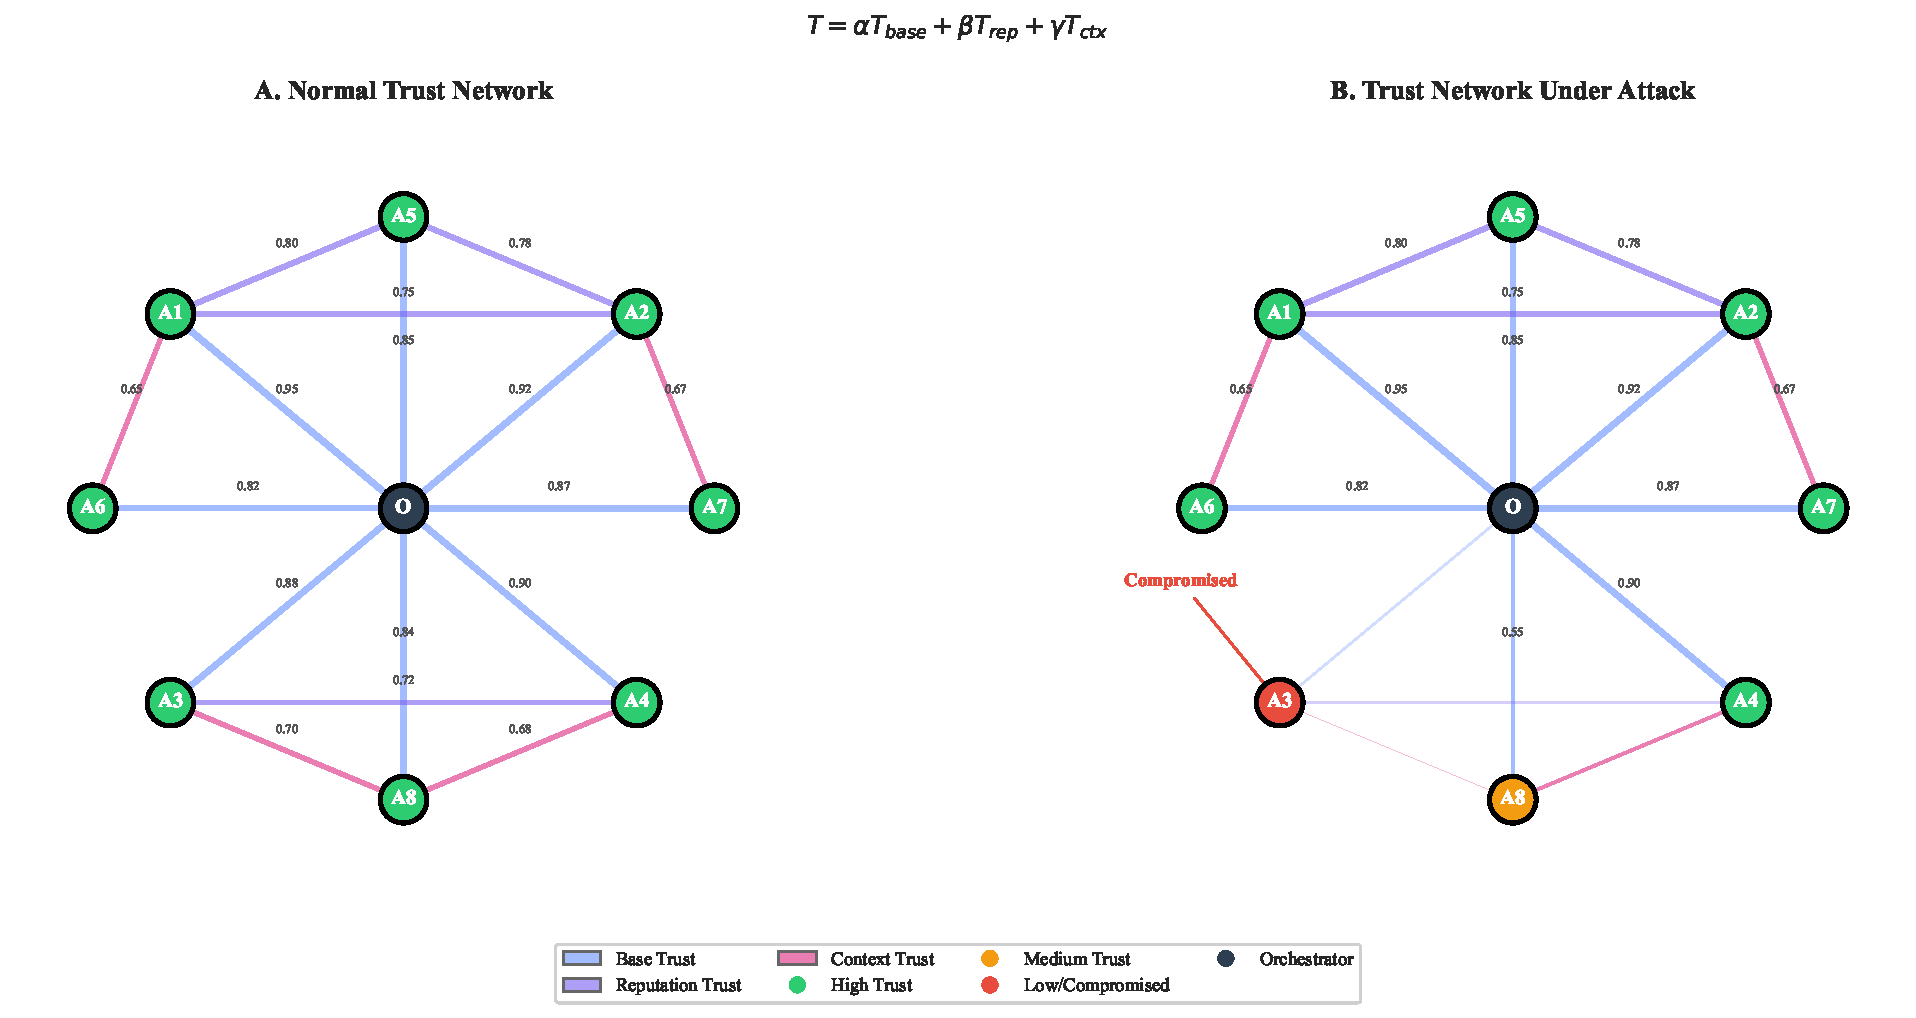
\includegraphics[width=0.9\textwidth]{../figures/trust_network.pdf}
\caption{Trust Network Topology: Directed graph showing trust relationships $\mathcal{T}_{i \to j}$ between agents in hierarchical (left) and peer-to-peer (right) configurations. Edge weights represent trust values in $[0,1]$; doubled arrows indicate bidirectional trust. Orchestrator $a_0$ occupies hub position in hierarchical topology.}
\label{fig:trust-network}
\end{figure}

\Cref{fig:trust-network} visualizes the trust relationships in a
representative multiagent operator. Edge weights represent trust scores
\(\mathcal{T}_{i \to j}\), with thicker edges indicating higher trust.
The network topology illustrates how trust propagates through delegation
chains and highlights potential attack surfaces for trust manipulation
attacks (\(\Omega_4\)).

\subsubsection{Trust Computation}\label{trust-computation}

\begin{definition}[Trust Function]
\label{def:trust-function}
Trust from agent $a_i$ to agent $a_j$ at time $t$:
\begin{equation}
\label{eq:trust-function}
\mathcal{T}_{i \to j}^t = \alpha \cdot T_{\text{base}}(j) + \beta \cdot T_{\text{rep}}^t(j) + \gamma \cdot T_{\text{ctx}}^t(i,j)
\end{equation}
subject to $\alpha + \beta + \gamma = 1$, with components in \cref{tab:trust-components}.
\end{definition}

\begin{table}[htbp]
\centering
\caption{Trust function components.}
\label{tab:trust-components}
\begin{tabular}{@{}llp{5cm}@{}}
\toprule
Component & Weight & Description \\
\midrule
$T_{\text{base}}$ & $\alpha$ & Architectural trust (role-based) \\
$T_{\text{rep}}$ & $\beta$ & Reputation (historical accuracy) \\
$T_{\text{ctx}}$ & $\gamma$ & Context (task-specific factors) \\
\bottomrule
\end{tabular}
\end{table}

\begin{remark}[Trust as Precision Weighting]
\label{rem:trust-precision}
The composite trust formula above is equivalent to precision-weighted
message integration from the Free Energy Principle: the composite score
$\mathcal{T}_{i\to j}$ is proportional to the precision $\rho_j$ with
which agent $i$ should weight messages from agent $j$ when updating its
posterior beliefs.  High-trust messages dominate the belief update;
low-trust messages contribute marginally.  This correspondence provides a
neurocomputational grounding for the trust calculus (Part~2, Theorem~FEP.2, ``Trust-Precision Duality'').
\end{remark}

\begin{definition}[Trust Delegation]
\label{def:trust-delegation}
When agent $a_i$ delegates trust through $a_j$ to $a_k$:
\begin{equation}
\label{eq:trust-delegation}
\mathcal{T}_{i \to k}^{\text{del}} = \min(\mathcal{T}_{i \to j}, \mathcal{T}_{j \to k}) \cdot \delta^d
\end{equation}
where $\delta \in (0, 1)$ is the decay factor and $d \in \mathbb{N}$ is the delegation depth.
\end{definition}

\subsubsection{Trust Algebra}\label{trust-algebra}

\emph{The trust algebra provides the mathematical foundation for
combining trust scores. The key insight is that trust through
intermediaries (delegation, \(\otimes\)) uses the minimum-then-decay
rule, while trust from multiple sources (aggregation, \(\oplus\)) uses
the maximum. This prevents both trust laundering and artificial
inflation.}

\begin{definition}[Trust Algebra]
\label{def:trust-algebra}
The trust algebra $(\mathcal{T}, \otimes, \oplus, 0, 1)$ comprises:
\begin{itemize}
\item \textbf{Domain}: $\mathcal{T} = [0, 1]$
\item \textbf{Delegation}: $T_1 \otimes T_2 = \min(T_1, T_2) \cdot \delta$ (sequential)
\item \textbf{Aggregation}: $T_1 \oplus T_2 = \max(T_1, T_2)$ (parallel)
\item \textbf{Zero}: $0$ (complete distrust)
\item \textbf{Unit}: $1$ (complete trust)
\end{itemize}
\end{definition}

\emph{The following theorem is the central security guarantee of the
trust calculus: it establishes that trust cannot be ``laundered''
through delegation chains. No matter how an adversary routes content
through trusted intermediaries, each hop reduces effective trust by
factor \(\delta\).}

\begin{theorem}[Trust Boundedness]
\label{thm:trust-bounded}
For any delegation chain of depth $d$:
\begin{equation}
\label{eq:trust-bound}
\mathcal{T}_{i \to k}^{\text{del}} \leq \delta^d
\end{equation}
\end{theorem}

\begin{proof}
By induction on $d$. \textbf{Base}: $d=0 \Rightarrow \mathcal{T} \leq 1$. \textbf{Step}: $\mathcal{T}^{d+1} = \min(\cdot) \cdot \delta \leq \delta^d \cdot \delta = \delta^{d+1}$.
\end{proof}

\begin{corollary}
\label{cor:no-amplification}
Trust cannot be amplified through delegation chains.
\end{corollary}

\begin{corollary}
\label{cor:trust-vanish}
Trust vanishes exponentially: $\lim_{d \to \infty} \mathcal{T}_{i \to k}^{\text{del}} = 0$.
\end{corollary}

\begin{figure}[htbp]
\centering
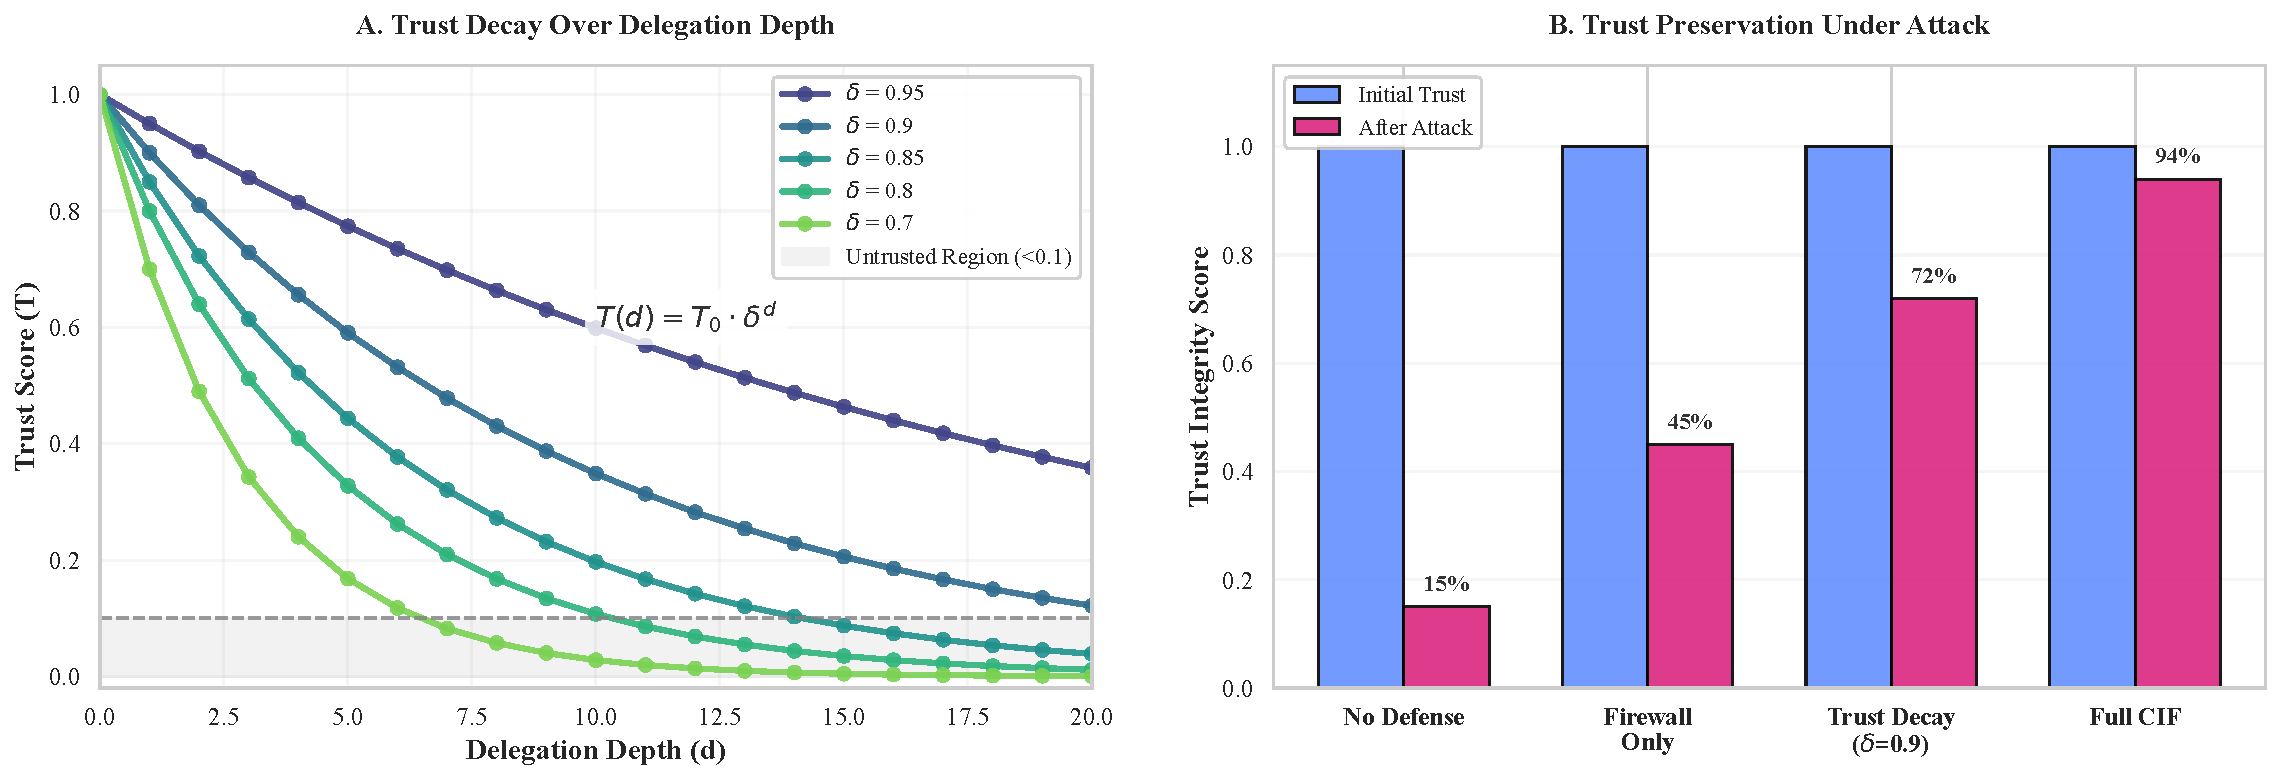
\includegraphics[width=0.9\textwidth]{../figures/trust_decay.pdf}
\caption{Trust Decay Over Delegation Depth: Exponential decay curves showing trust attenuation $\mathcal{T}_{\text{del}}^{(d)} = \delta^d \cdot \mathcal{T}_{i \to j}$ for decay factors $\delta \in \{0.5, 0.7, 0.8, 0.9\}$ over delegation chains of depth $d = 1$ to $10$. At $\delta = 0.8$, trust falls below $\tau=0.5$ at depth 4 and below $\tau=0.1$ at depth 11 (outside this plotted range). \textit{Note: Values are illustrative examples demonstrating the mathematical framework; specific decay factors should be tuned to deployment context.}}
\label{fig:trust-decay}
\end{figure}

\Cref{fig:trust-decay} visualizes the exponential decay of trust across
delegation depth for various decay factors \(\delta\), demonstrating how
the bounded delegation mechanism (\cref{thm:trust-bounded}) prevents
trust amplification.

\begin{figure}[htbp]
\centering
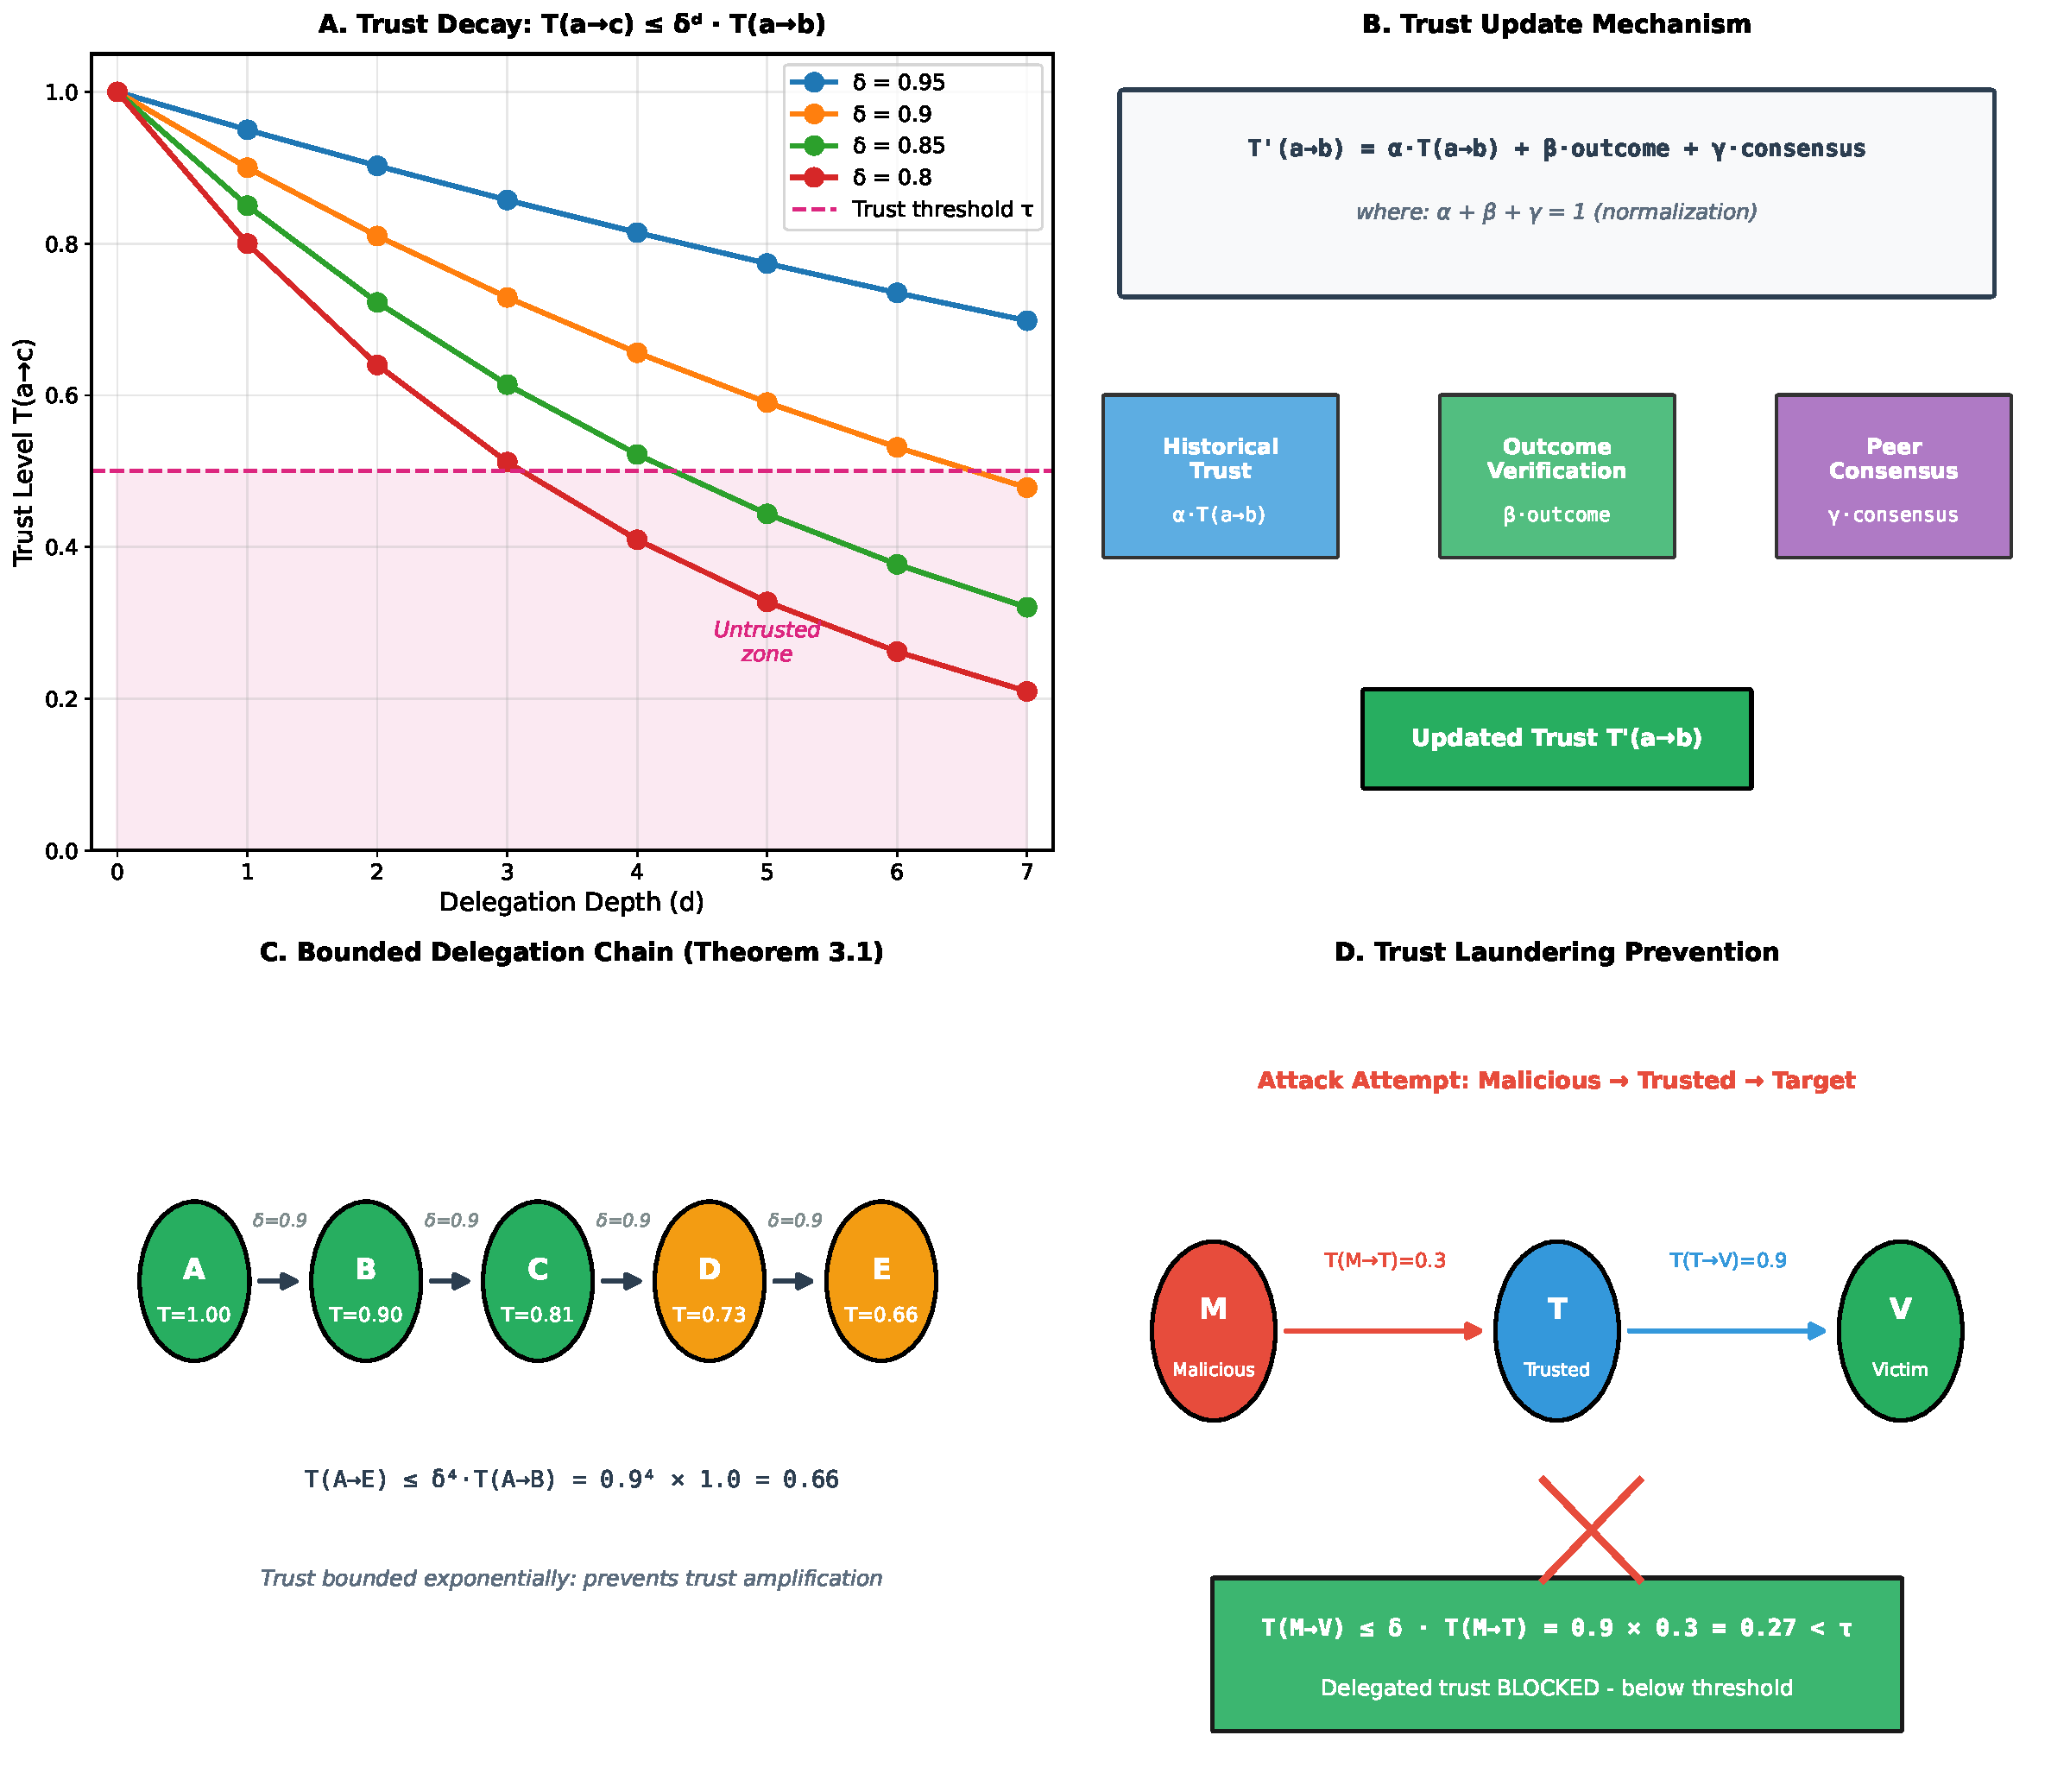
\includegraphics[width=1.0\textwidth]{../figures/trust_calculus_comprehensive.pdf}
\caption{Trust Calculus Comprehensive: Complete trust calculus framework showing initialization matrices, update rules (direct experience, reputation, recommendation), decay mechanics, and the no-amplification invariant. The composition rule $\mathcal{T}_{i \to k} = \delta \cdot \min(\mathcal{T}_{i \to j}, \mathcal{T}_{j \to k})$ ensures trust cannot be manufactured through delegation chains.}
\label{fig:trust-calculus-comprehensive}
\end{figure}

\Cref{fig:trust-calculus-comprehensive} presents the complete trust
calculus mechanics across four panels. Panel A demonstrates the trust
decay function
\(\mathcal{T}(a \to c) \leq \delta^d \cdot \mathcal{T}(a \to b)\) for
decay factors \(\delta \in \{0.8, 0.85, 0.9, 0.95\}\), showing how trust
falls below threshold \(\tau = 0.5\) at different delegation depths.
Panel B formalizes the trust update mechanism
\(\mathcal{T}'(a \to b) = \alpha \cdot \mathcal{T}(a \to b) + \beta \cdot \text{outcome} + \gamma \cdot \text{consensus}\)
where \(\alpha + \beta + \gamma = 1\), integrating historical trust,
outcome verification, and peer consensus. Panel C illustrates a bounded
delegation chain (Theoremabout \ref{thm:trust-bounded}):
starting from \(\mathcal{T}(A \to B) = 1.0\) with \(\delta = 0.9\),
trust decays through agents B, C, D to E with
\(\mathcal{T}(A \to E) = 0.9^4 \times 1.0 = 0.66\). Panel D demonstrates
trust laundering prevention: a malicious agent M with
\(\mathcal{T}(M \to T) = 0.3\) attempting to exploit trusted
intermediary T with \(\mathcal{T}(T \to V) = 0.9\) cannot achieve
sufficient delegated trust since
\(\mathcal{T}(M \to V) \leq 0.9 \times 0.3 = 0.27 < \tau\), blocking the
attack.

\begin{theorem}[Delegation Associativity]
\label{thm:delegation-assoc}
The sequential delegation operation is defined by
\(T_1 \otimes T_2 = \delta\min(T_1,T_2)\). Because the decay factor is
applied at each composition step, this operation is not associative in
general; chain evaluation therefore preserves the explicit left-to-right
delegation order.
\begin{equation}
\label{eq:delegation-assoc}
T_1 \otimes (T_2 \otimes T_3) \neq (T_1 \otimes T_2) \otimes T_3
\end{equation}
\end{theorem}

\begin{proof}
For example, with $(T_1,T_2,T_3,\delta)=(0.9,0.9,0.1,0.9)$, the left-associated
value is $0.090$ while the right-associated value is $0.081$. Thus any
associative abstraction must be defined separately (for example, as a chain
functional $\min_i T_i\,\delta^d$), rather than inferred for $\otimes$.
\end{proof}

\begin{theorem}[Aggregation Properties]
\label{thm:aggregation}
Trust aggregation $\oplus$ satisfies: (i) associativity, (ii) commutativity, (iii) idempotence, (iv) identity $T \oplus 0 = T$, and (v) absorption $T \oplus 1 = 1$.
\end{theorem}

\begin{theorem}[No Trust Amplification]
\label{thm:no-trust-amp}
For any path $p = (a_0, \ldots, a_k)$:
\begin{equation}
\label{eq:no-amplification}
\mathcal{T}_{a_0 \to a_k}^{\text{path}} \leq \min_{i \in [0,k-1]} \mathcal{T}_{a_i \to a_{i+1}}
\end{equation}
A proof of the no-amplification claim is given in the supplementary material
(\cref{thm:trust-amp-restated}, S01), which states the identical bound under
a dedicated label.
\end{theorem}

\begin{theorem}[Trust Monotonicity]
\label{thm:trust-monotonic}
Delegation is monotonic: $T_1 \leq T_1' \land T_2 \leq T_2' \Rightarrow T_1 \otimes T_2 \leq T_1' \otimes T_2'$.
\end{theorem}

\subsubsection{Cross-Modality Trust}\label{sec:cross-modality-trust}

When agents operate across modalities---processing text, code, images,
audio, and structured data---trust must account for modality-specific
reliability and attack susceptibility.

\begin{definition}[Modality Trust Adjustment]
\label{def:modality-trust}
For agent $a_j$ operating in modality $m$, the adjusted trust from agent $a_i$ is:
\begin{equation}
\label{eq:modality-trust}
\mathcal{T}_{i \to j}^{m} = \mathcal{T}_{i \to j} \cdot \eta_m
\end{equation}
where $\eta_m \in (0, 1]$ is the modality reliability factor.
\end{definition}

\begin{table}[htbp]
\centering
\caption{Recommended modality reliability factors.}
\label{tab:modality-factors}
\begin{tabular}{@{}llp{5cm}@{}}
\toprule
Modality $m$ & $\eta_m$ & Rationale \\
\midrule
Text (verified source) & 1.0 & Baseline modality \\
Code (compilable) & 0.95 & Syntax verification possible \\
Structured data (schema-valid) & 0.90 & Schema provides partial verification \\
Text (external) & 0.80 & Injection risk \\
Images & 0.70 & Adversarial perturbation vulnerability \\
Audio & 0.65 & Ultrasonic injection, splicing attacks \\
Video & 0.60 & Combines image and temporal vulnerabilities \\
\bottomrule
\end{tabular}
\end{table}

\begin{theorem}[Cross-Modality Delegation Bound]
\label{thm:cross-modality-bound}
For delegation chain crossing modalities $m_1, \ldots, m_k$:
\begin{equation}
\label{eq:cross-modality-bound}
\mathcal{T}_{i \to j}^{\text{cross}} \leq \delta^d \cdot \prod_{l=1}^{k} \eta_{m_l}
\end{equation}
\end{theorem}

This ensures that trust degradation compounds across both delegation
depth and modality transitions, preventing adversaries from laundering
low-trust content through modality boundaries.

\subsubsection{Federated Trust}\label{sec:federated-trust}

In enterprise deployments, multiagent systems increasingly span
organizational boundaries. A financial services orchestrator might
delegate to a risk assessment system from one vendor, a compliance
checker from another, and market data feeds from multiple providers.
\textbf{Federated trust} addresses how to reason about trust across
these boundaries.

\begin{definition}[Trust Domain]
\label{def:trust-domain}
A trust domain $\mathcal{D}$ is a set of agents sharing a common trust authority and consistent trust semantics.
\end{definition}

\begin{definition}[Cross-Domain Trust]
\label{def:cross-domain-trust}
For agent $a_i$ in domain $\mathcal{D}_1$ and agent $a_j$ in domain $\mathcal{D}_2$:
\begin{equation}
\label{eq:cross-domain-trust}
\mathcal{T}_{i \to j}^{\text{fed}} = \mathcal{T}_{i \to \mathcal{D}_2} \cdot \mathcal{T}_{\mathcal{D}_2}(j)
\end{equation}
where $\mathcal{T}_{i \to \mathcal{D}_2}$ is $a_i$'s trust in domain $\mathcal{D}_2$ and $\mathcal{T}_{\mathcal{D}_2}(j)$ is $a_j$'s standing within its domain.
\end{definition}

This two-stage model captures realistic trust reasoning: an organization
might trust a vendor (domain trust) differently than individual agents
within that vendor (agent trust).

\begin{property}[Federated Trust Bound]
\label{prop:federated-bound}
Cross-domain trust is bounded by domain trust:
\begin{equation}
\label{eq:federated-bound}
\mathcal{T}_{i \to j}^{\text{fed}} \leq \mathcal{T}_{i \to \mathcal{D}_2}
\end{equation}
ensuring that untrusted domains cannot boost individual agent trust.
\end{property}

Federated trust introduces additional challenges that remain open
research problems:

\begin{itemize}
\item \textbf{Trust semantics heterogeneity}: Different domains may use incompatible trust scales or update rules
\item \textbf{Trust attestation}: How can domains cryptographically attest to their internal trust assessments?
\item \textbf{Privacy-preserving trust}: Can trust be verified without revealing sensitive internal assessments?
\end{itemize}

\subsubsection{Belief Update Semantics}\label{sec:belief-update-rules}

\begin{definition}[Evidence Structure]
\label{def:evidence}
Evidence is a tuple $e = \langle \phi, c, s, \pi \rangle$ comprising proposition $\phi$, confidence $c \in [0,1]$, source $s$, and provenance chain $\pi$.
\end{definition}

\begin{definition}[Trust-Weighted Bayesian Update]
\label{def:bayesian-update}
Upon receiving evidence $e$ from source $s$:
\begin{equation}
\label{eq:bayesian-update}
\mathcal{B}_i^{t+1}(\phi) = \frac{\mathcal{B}_i^t(\phi) \cdot \left[\mathcal{T}_{i \to s} P(e|\phi) + (1-\mathcal{T}_{i \to s})P_0(e|\phi)\right]}{\sum_{\psi} \mathcal{B}_i^t(\psi) \cdot \left[\mathcal{T}_{i \to s} P(e|\psi) + (1-\mathcal{T}_{i \to s})P_0(e|\psi)\right]}
\end{equation}
Trust mixes the source likelihood with a neutral likelihood $P_0$; low-trust sources therefore have a diminished update impact rather than canceling as a common normalization factor.
\end{definition}

\textbf{Rule B-Direct} (Direct Evidence): \begin{equation}
\label{eq:rule-direct}
\frac{e = \langle \phi, c, s, \pi \rangle \quad V(\pi) = 1 \quad \mathcal{T}_{i \to s} \geq \tau_{\text{trust}}}{\mathcal{B}_i^{t+1}(\phi) = \text{BayesUpdate}(\mathcal{B}_i^t(\phi), c \cdot \mathcal{T}_{i \to s})}
\end{equation}

\textbf{Rule B-Delegated} (Delegated Evidence): evidence received
through a delegation chain of depth \(d\) is accepted only when its
provenance is valid and its delegated trust meets the configured
threshold: \begin{equation}
\label{eq:rule-delegated}
\frac{e = \langle \phi, c, s, \pi \rangle \quad V(\pi) = 1 \quad
\mathcal{T}^{\mathrm{del}}_{i \to s} = \mathcal{T}^{(d)}_{i \to s} \geq \tau_{\text{trust}}}
{\mathcal{B}_i^{t+1}(\phi) = \operatorname{BayesUpdate}
\left(\mathcal{B}_i^t(\phi), c \cdot \mathcal{T}^{\mathrm{del}}_{i \to s}\right)}.
\end{equation} Here \(\mathcal{T}^{(d)}_{i \to s} \leq \delta^d\) is the
delegated trust after \(d\) hops, making depth-dependent attenuation
explicit.

\textbf{Rule B-Corroboration} (Multiple Sources): \begin{equation}
\label{eq:rule-corroboration}
\frac{\{e_j\}_{j=1}^k: \forall j.\, e_j = \langle \phi, c_j, s_j, \pi_j \rangle \quad |\{s_j\}| \geq \kappa}{\mathcal{B}_i^{t+1}(\phi) = 1 - \prod_{j=1}^{k}(1 - c_j \cdot \mathcal{T}_{i \to s_j})}
\end{equation}

\begin{lemma}[Belief Boundedness]
\label{lem:belief-bounded}
After any update sequence: $\forall \phi: 0 \leq \mathcal{B}_i(\phi) \leq 1$.
\end{lemma}

\subsubsection{Sandboxed Belief Model}\label{sec:sandbox-rules}

\begin{definition}[Sandboxed Beliefs]
\label{def:sandbox}
Beliefs from unverified sources enter provisional state:
\begin{equation}
\label{eq:sandbox-partition}
\mathcal{B}_i = \mathcal{B}_{\text{verified}} \cup \mathcal{B}_{\text{provisional}}
\end{equation}
\end{definition}

\textbf{Rule S-Sandbox} (Enter Sandbox): \begin{equation}
\label{eq:rule-sandbox}
\frac{e = \langle \phi, c, s, \pi \rangle \quad (\mathcal{T}_{i \to s} < \tau_{\text{trust}} \lor V(\pi) = 0)}{\mathcal{B}_{\text{prov}} \gets \mathcal{B}_{\text{prov}} \cup \{(\phi, c, s, \pi, \text{TTL})\}}
\end{equation}

\textbf{Rule S-Promote} (Sandbox Promotion): \begin{equation}
\label{eq:rule-promote}
\frac{(\phi, \ldots) \in \mathcal{B}_{\text{prov}} \quad V(\pi) = 1 \quad \text{Consistent}(\mathcal{B}_{\text{ver}} \cup \{\phi\}) \quad |\text{Corr}(\phi)| \geq \kappa}{\mathcal{B}_{\text{ver}} \gets \mathcal{B}_{\text{ver}} \cup \{\phi\}; \quad \mathcal{B}_{\text{prov}} \gets \mathcal{B}_{\text{prov}} \setminus \{(\phi, \ldots)\}}
\end{equation}

\textbf{Rule S-Expire} (Sandbox Expiry): \begin{equation}
\label{eq:rule-expire}
\frac{(\phi, c, s, \pi, \text{TTL}) \in \mathcal{B}_{\text{prov}} \quad \text{TTL} \leq 0}{\mathcal{B}_{\text{prov}} \gets \mathcal{B}_{\text{prov}} \setminus \{(\phi, c, s, \pi, \text{TTL})\}}
\end{equation}

Promotion requires: (1) provenance verification \(V(\pi) = 1\), (2)
consistency with verified beliefs, and (3) corroboration threshold
\(\kappa\).

\subsection{Information-Theoretic Detection
Bounds}\label{sec:detection-bounds}

\emph{Having established the trust calculus (how agents reason about
each other) and belief update semantics (how agents incorporate
information), we now turn to fundamental limits on attack detection.
This section establishes fundamental limits on what any detection system
can achieve. Like Shannon's channel capacity in communications, these
bounds are not limitations of specific mechanisms but mathematical
constraints on what is possible.}

\begin{definition}[Attack Information Channel]
\label{def:attack-channel}
An attack models a communication channel from adversary to target:
\begin{equation}
\label{eq:attack-channel}
\text{Channel}: \mathcal{A}_{\text{adv}} \to \sigma_{\text{target}}
\end{equation}
\end{definition}

\begin{theorem}[Minimum Attack Entropy]
\label{thm:min-entropy}
For attack $\mathcal{A}$ to succeed with probability $p$:
\begin{equation}
\label{eq:min-entropy}
H(\mathcal{A}) \geq -\log_2(1-p) + H(\sigma_{\text{target}}|\mathcal{A})
\end{equation}
\end{theorem}

\begin{proof}
By the data processing inequality. The attack must contain sufficient information to change the target state.
\end{proof}

\begin{corollary}
\label{cor:low-entropy-detectable}
Attacks with low entropy (simple patterns) are more detectable.
\end{corollary}

\begin{definition}[Detector Information Gain]
\label{def:detector-gain}
For detector $D$ observing system state $S$:
\begin{equation}
\label{eq:detector-gain}
I(D; \mathcal{A}) = H(\mathcal{A}) - H(\mathcal{A}|D(S))
\end{equation}
\end{definition}

\begin{theorem}[Fundamental Detection Limit]
\label{thm:detection-limit}
No detector achieves detection rate $r$ if:
\begin{equation}
\label{eq:detection-limit}
r > \frac{I(D; \mathcal{A})}{H(\mathcal{A})}
\end{equation}
\end{theorem}

\emph{The following theorem captures the fundamental tradeoff facing
attackers: high-impact attacks are easier to detect, while stealthy
attacks have limited effect. This is not a limitation of our
defenses---it is a mathematical constraint that any attack must
satisfy.}

\begin{theorem}[Stealth-Impact Tradeoff]
\label{thm:stealth-impact}
For attack with impact $\mathcal{I}$ and stealth $\mathcal{S}$ (inverse detectability):
\begin{equation}
\label{eq:stealth-impact}
\mathcal{I} \cdot \mathcal{S} \leq C_{\text{channel}}
\end{equation}
where $C_{\text{channel}}$ is the attack channel capacity.
\end{theorem}

\begin{remark}[Geometric Sharpening of the Stealth-Impact Bound]
\label{rem:geometric-bound}
Theorem~\ref{thm:stealth-impact} can be sharpened using the information
geometry of the belief manifold (Part~2, Supplement~S10).  When belief
space is endowed with the Fisher-Rao metric
$G_{ij}(p) = \delta_{ij}/p_i$ \cite{amari2000methods}, the Fisher-Rao geodesic distance
\[
d_{\mathrm{FR}}(p, q) = 2\arccos\!\left(\sum_i \sqrt{p_i q_i}\right)
\]
measures the geometric ``distance'' of an attack.  Impact $\mathcal{I}$
is proportional to $d_{\mathrm{FR}}(p_0, p_{\text{attacked}})$, while
stealth $\mathcal{S}$ is inversely proportional to the same quantity.
The curvature of the probability simplex $Delta^{n-1}$ (constant
positive curvature $kappa = n(n-1)/4$) implies that the product
$\mathcal{I} \cdot \mathcal{S}$ is bounded by the diameter of the manifold:
\[
\mathcal{I} \cdot \mathcal{S} \leq \frac{\pi}{2},
\]
since $d_{\mathrm{FR}} <= pi$ (Hellinger antipodal distributions).
This recovers $C_{\text{channel}} = pi/2$ as the tight bound when impact
is measured in natural (Fisher-Rao) units. It is a geometric \emph{argument}
for the constant in Theorem~\ref{thm:stealth-impact}, not a proof of that
theorem: the theorem itself is stated without proof and is recorded as
deferred in the proof-status index (S01, \cref{sec:proof-status}), and the
curvature step above assumes the impact measure is the Fisher-Rao distance
rather than deriving that identification.
Furthermore, the connection to KL divergence---$D_{\mathrm{KL}}(p \,\|\, p')
about \tfrac{1}{2}(Delta p)^\top G(p)(Delta p)$ for small
perturbations---gives geometric justification for the drift detection
threshold $theta_{\text{drift}} = 0.3$: this corresponds to a
Fisher-Rao step of approximately $0.775$ radians, or roughly $25\%$ of
the maximum possible attack distance ($r_theta = \sqrt{2\,theta_{\text{drift}}} = \sqrt{0.6}$).
\end{remark}

\begin{table}[htbp]
\centering
\caption{Information-theoretic bounds by attack type.}
\label{tab:attack-bounds}
\begin{tabular}{@{}lll@{}}
\toprule
Attack Type & Min Entropy $H(\mathcal{A})$ & Detection Lower Bound \\
\midrule
Belief Injection & $\log_2 |\Phi|$ & $\frac{\log_2 |\Phi|}{H(\mathcal{B})}$ \\
Goal Hijacking & $H(\mathcal{G}_{\text{target}})$ & $\frac{H(\mathcal{G}_{\text{target}})}{H(\mathcal{G})}$ \\
Trust Manipulation & $\log_2 n$ & $\frac{\log_2 n}{H(\mathcal{T})}$ \\
Progressive Drift & $T \cdot \log_2(1/delta_{\text{step}})$ & $\frac{T}{w} \cdot delta_{\text{step}}$ \\
\bottomrule
\end{tabular}
\end{table}

\begin{theorem}[Progressive Attack Detection Bound]
\label{thm:progressive-detection}
For progressive drift attack with step size $delta$ over $T$ steps:
\begin{equation}
\label{eq:progressive-bound}
P(\text{detect within } w \text{ steps}) \leq 1 - \left(1 - \frac{\delta}{\theta_{\text{step}}}\right)^{w}
\end{equation}
\end{theorem}

\begin{corollary}
\label{cor:small-steps}
Smaller step sizes exponentially reduce detection probability but require more time for impact.
\end{corollary}

\begin{definition}[Defense Information Budget]
\label{def:defense-budget}
Total monitoring capacity: $B_{\text{total}} = \sum_{d \in \mathcal{D}} B_d$.
\end{definition}

\begin{theorem}[Optimal Budget Allocation]
\label{thm:optimal-allocation}
Given attack distribution $P(\mathcal{A}_k)$ and detector sensitivities $\eta_d(\mathcal{A}_k)$:
\begin{equation}
\label{eq:optimal-allocation}
B_d^* = \frac{\sum_k P(\mathcal{A}_k) \cdot \eta_d(\mathcal{A}_k)}{\sum_{d'}\sum_k P(\mathcal{A}_k) \cdot \eta_{d'}(\mathcal{A}_k)} \cdot B_{\text{total}}
\end{equation}
\end{theorem}

\begin{proof}
Lagrangian optimization maximizing expected detection subject to budget constraint.
\end{proof}

\begin{figure}[htbp]
\centering
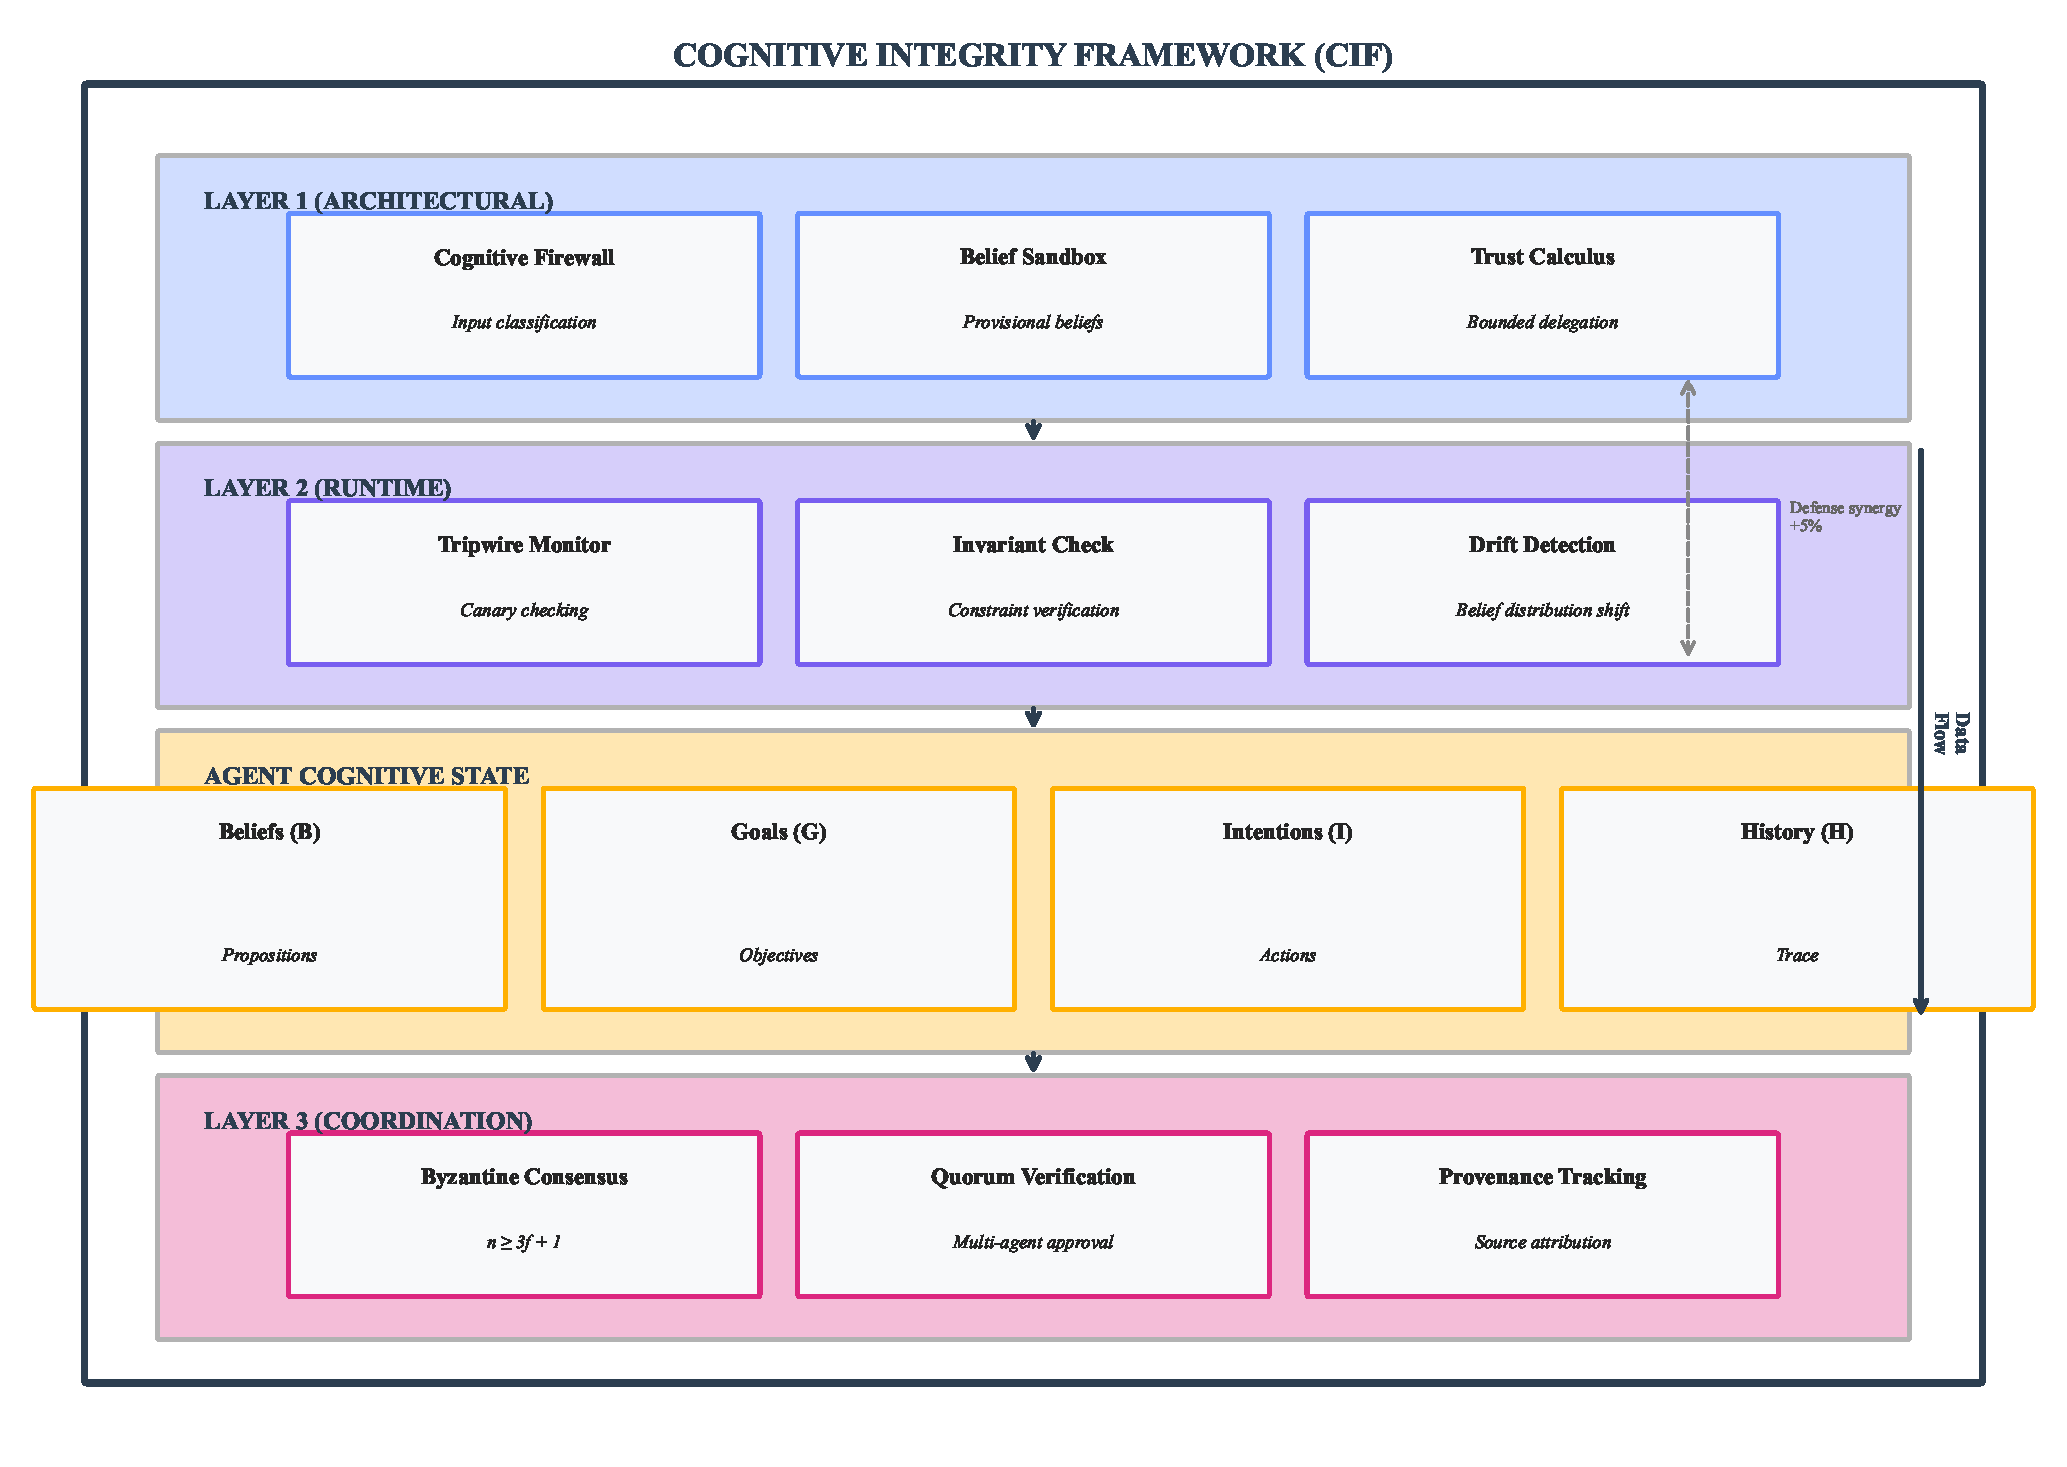
\includegraphics[width=1.0\textwidth]{../figures/cif_architecture.pdf}
\caption{CIF Architecture Overview: Three-layer defense architecture---\textbf{Layer 1} (Architectural): Cognitive Firewall at entry, Belief Sandbox for unverified data, Trust Calculus for delegation; \textbf{Layer 2} (Runtime): Tripwires for belief monitoring, Invariant verification, Drift detection; \textbf{Layer 3} (Coordination): Byzantine consensus, Quorum verification, Provenance tracking.}
\label{fig:cif-architecture}
\end{figure}

\Cref{fig:cif-architecture} presents the layered CIF architecture with
architectural defenses (left), runtime defenses (center), and
coordination mechanism (right). \Cref{fig:cif-comprehensive} expands
this to show data flow, attack interception points, and defense
composition.

\begin{figure}[htbp]
\centering
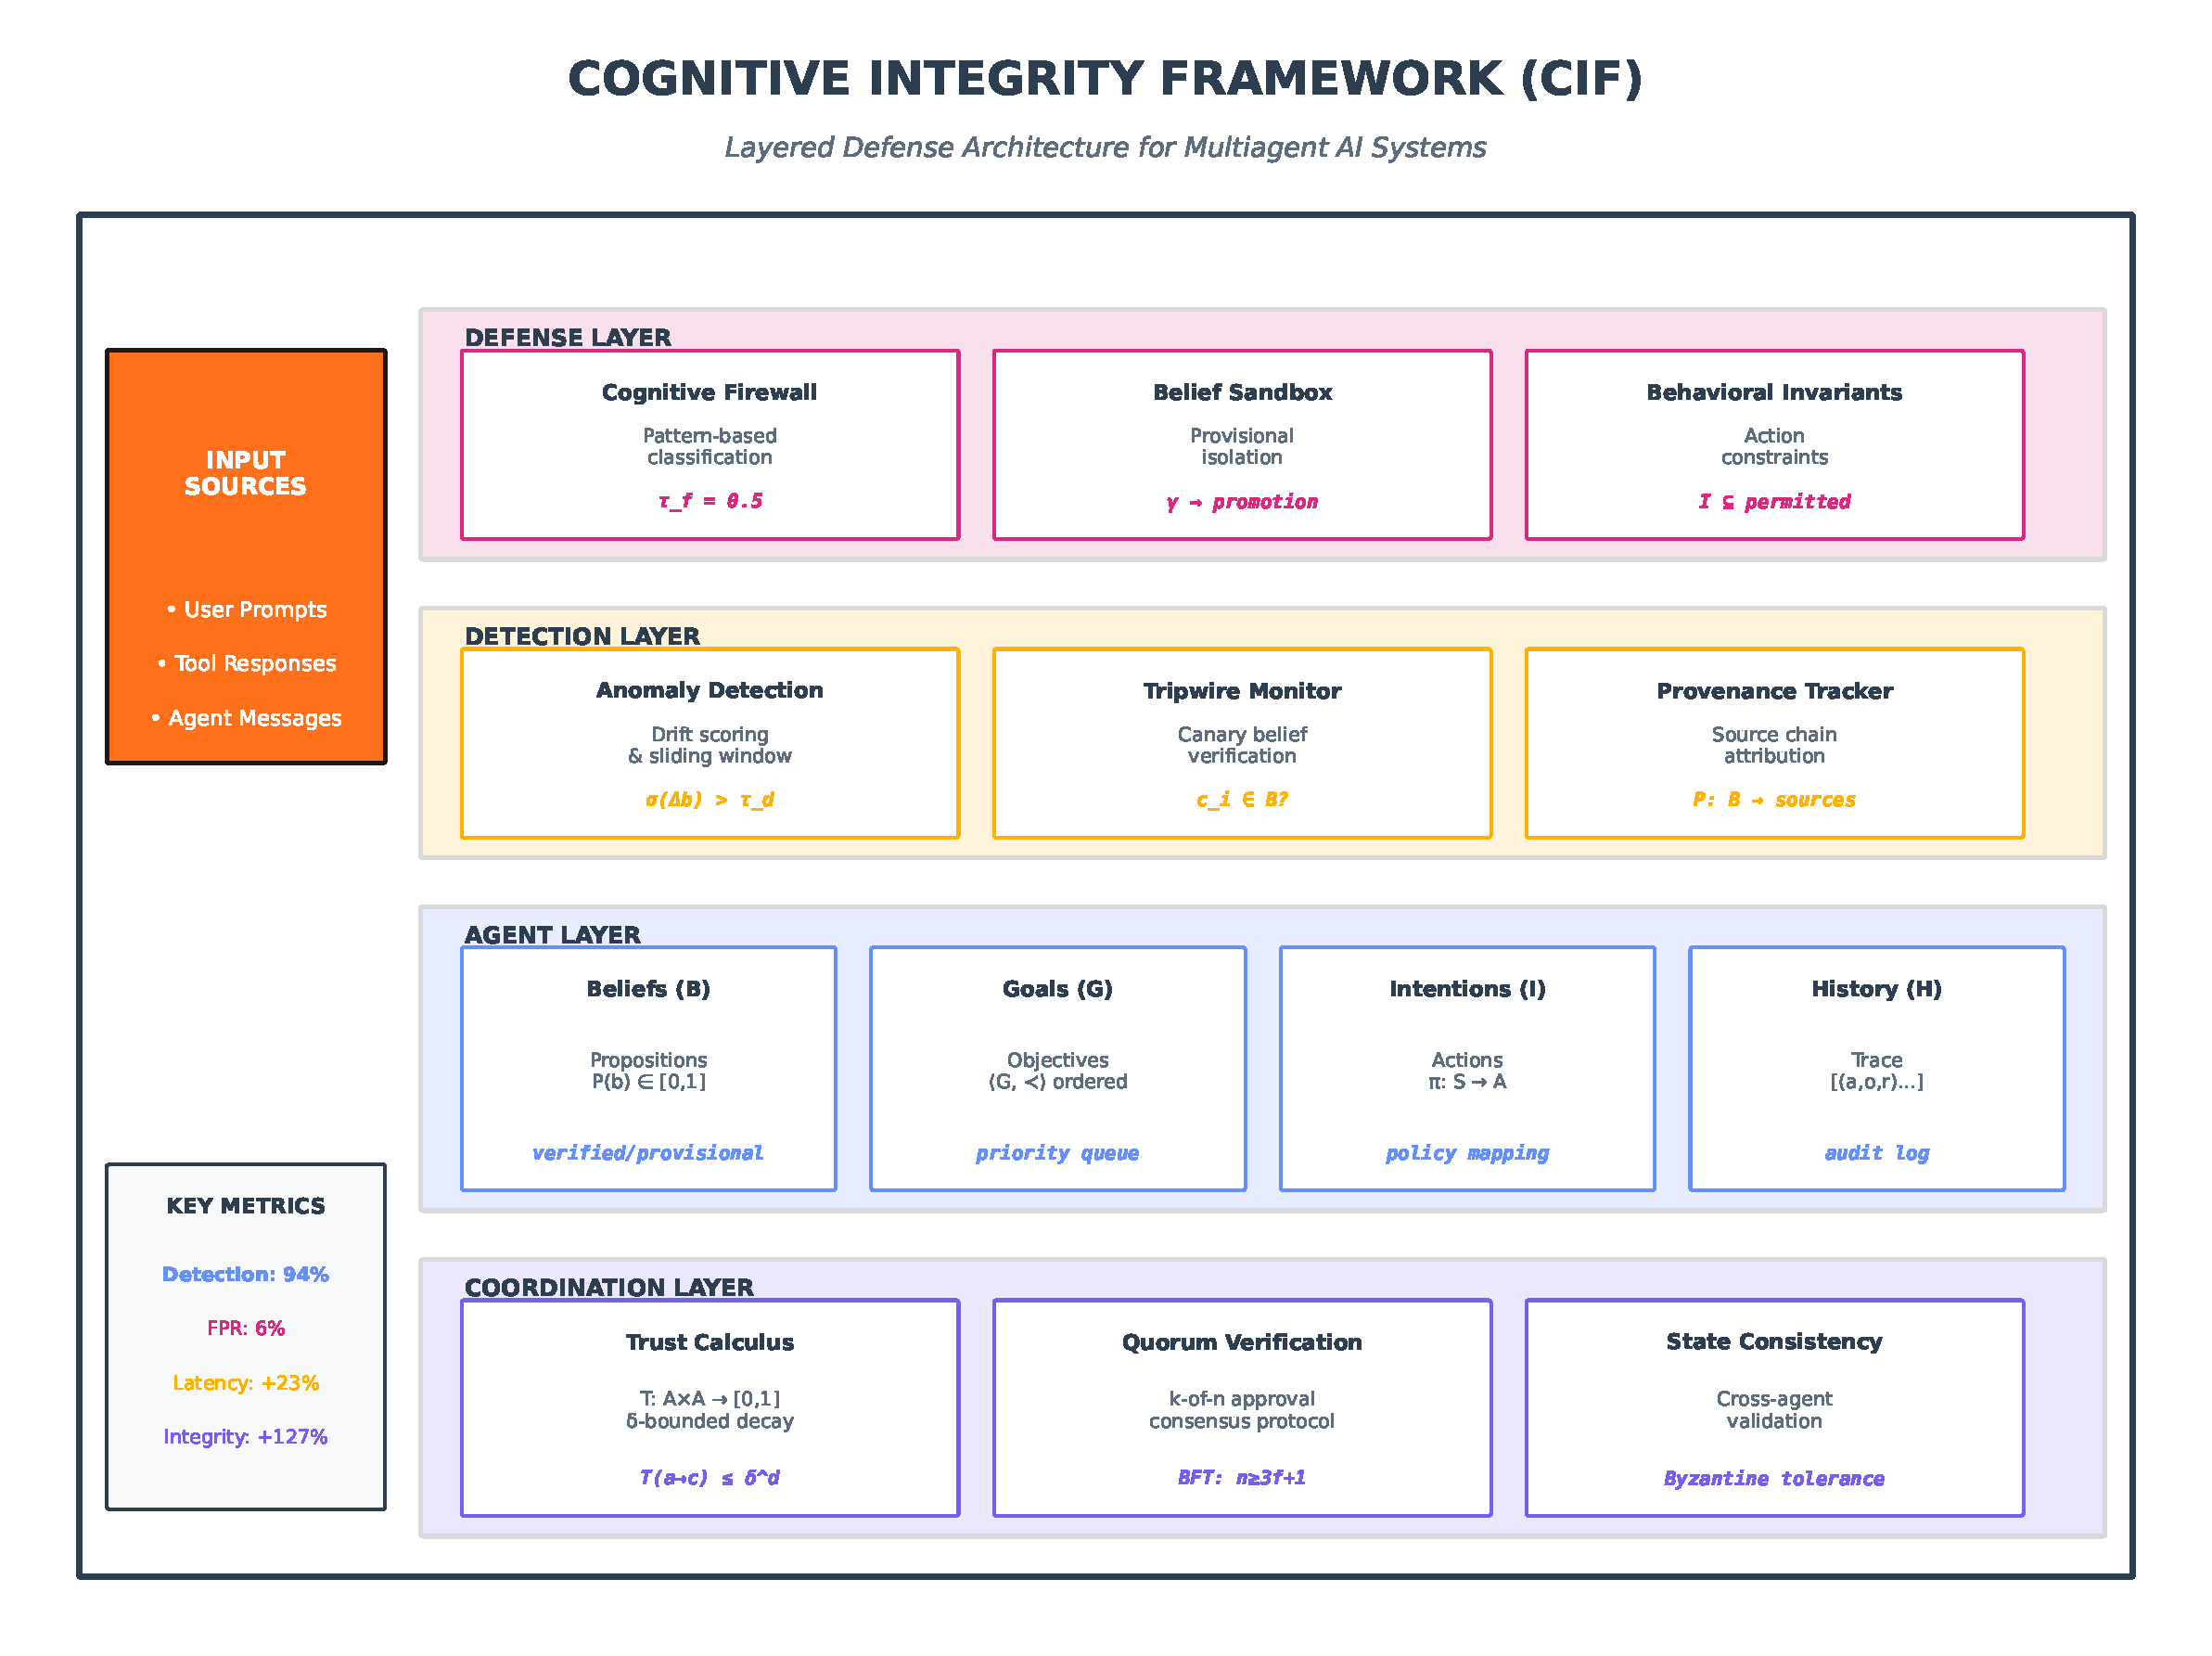
\includegraphics[width=1.0\textwidth]{../figures/cif_comprehensive.pdf}
\caption{Comprehensive CIF Architecture: Extended architecture showing data flow from user input through all defense layers to agent output. Attack interception points labeled $\Omega_1$--$\Omega_5$ indicate where each adversary class is detected. Defense composition follows multiplicative detection rate improvement (\cref{cor:layered-defense}).}
\label{fig:cif-comprehensive}
\end{figure}

\Cref{fig:cif-comprehensive} provides a detailed view of the complete
CIF architecture, including all component formulas and their
interactions. The defense layer implements the cognitive firewall with
threshold \(\tau_f = 0.5\), the belief sandbox with promotion function
\(\gamma\), and behavioral invariants constraining intentions
\(\mathcal{I} \subseteq \text{permitted}\). The detection layer
specifies anomaly scoring \(\sigma(\Delta b) > \tau_d\), tripwire
verification \(c_i \in \mathcal{B}?\), and provenance tracking
\(P: \mathcal{B} \to \text{sources}\). The coordination layer encodes
the trust calculus
\(\mathcal{T}: \mathcal{A} \times \mathcal{A} \to [0,1]\) with
\(\delta\)-bounded decay, k-of-n quorum protocols, and Byzantine fault
tolerance (\(n \geq 3f + 1\)). For empirical validation of detection
rates and performance overhead, see Part 2 of this series.

\subsection{CIF-AD Integration: Action-Delegation
Coupling}\label{sec:cif-ad-coupling}

\begin{figure}
\centering
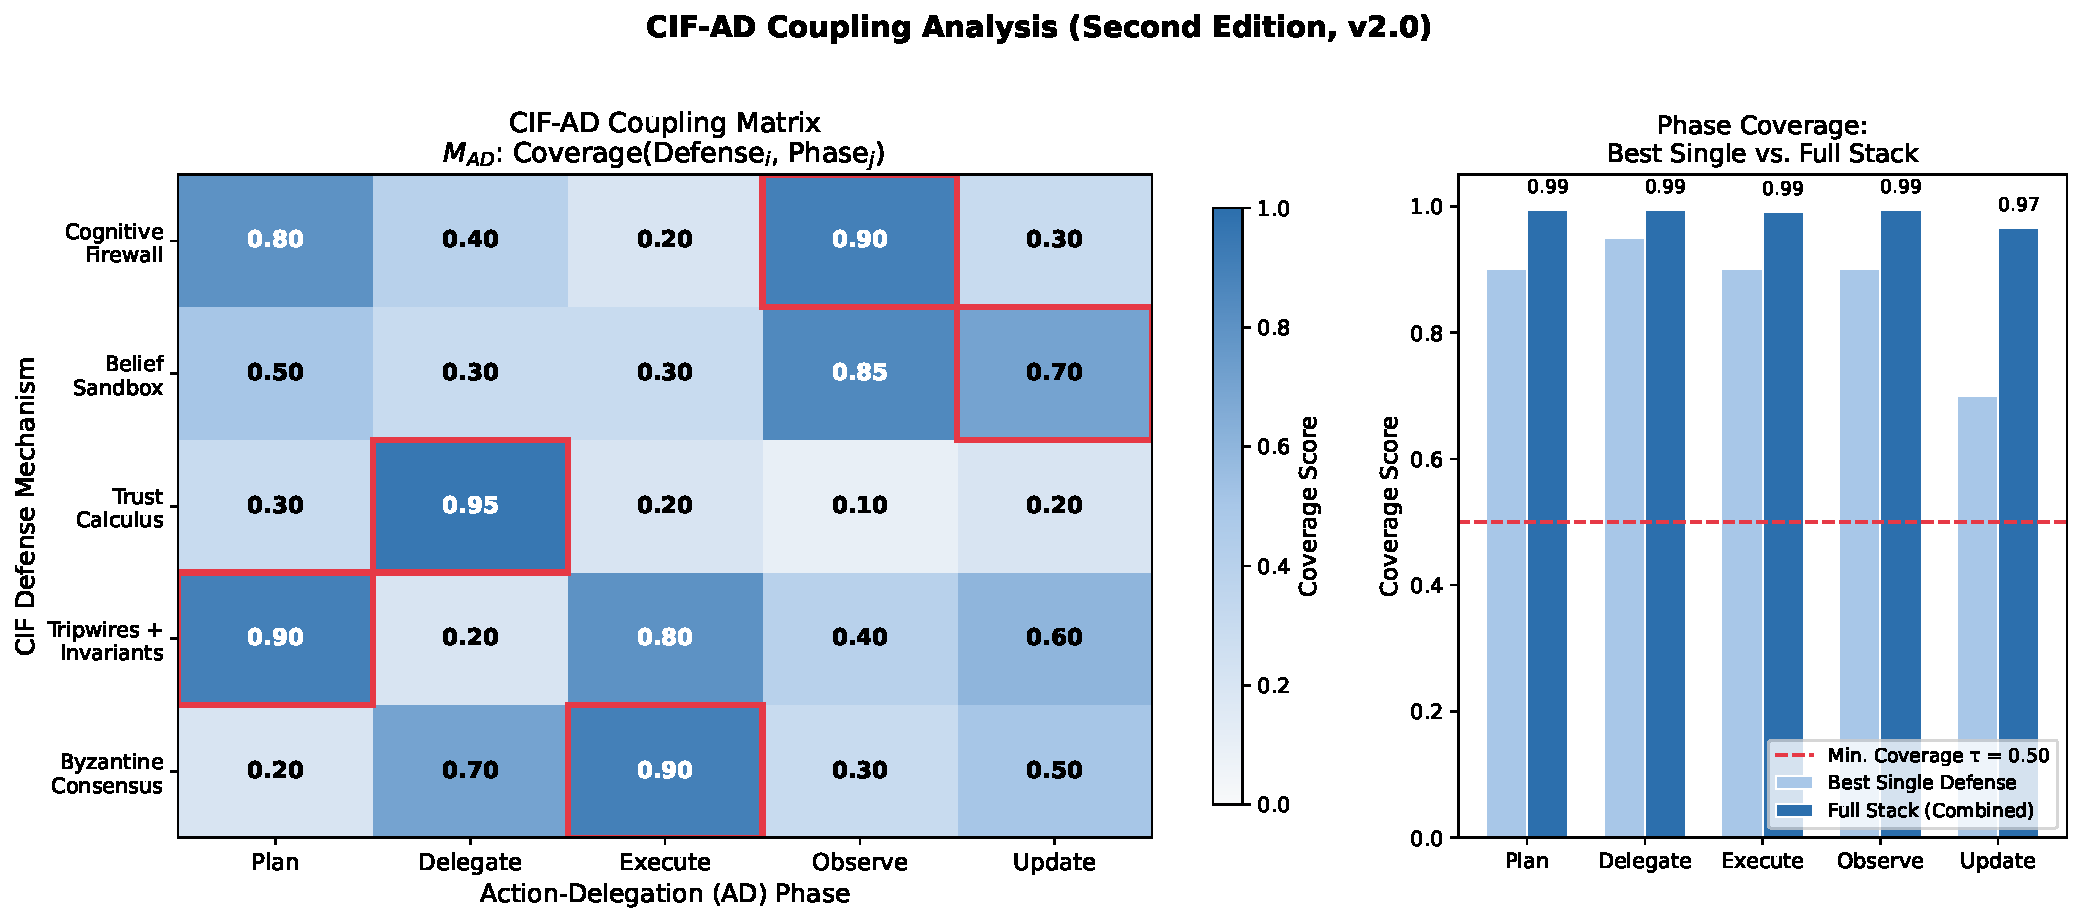
\includegraphics[width=0.85\linewidth,height=0.5\textheight,keepaspectratio,alt={CIF-AD action--delegation coupling matrix showing how Functional Requirements map to Design Parameters and delegation actions, making explicit where a Goal-Hijacking transient can introduce off-diagonal coupling.}]{../figures/cif_ad_coupling.pdf}
\caption{CIF-AD action--delegation coupling matrix showing how
Functional Requirements map to Design Parameters and delegation actions,
making explicit where a Goal-Hijacking transient can introduce
off-diagonal coupling.}\label{fig:cif-ad-coupling}
\end{figure}

\emph{The Cognitive Integrity Framework provides static structural
guarantees (trust bounds, belief consistency). But multiagent operators
are dynamic: agents act, delegate, and observe outcomes. This section
formalizes how CIF integrates with the Action-Delegation (AD) cycle to
provide continuous runtime security guarantees.}

\subsubsection{The Action-Delegation
Cycle}\label{the-action-delegation-cycle}

\begin{definition}[Action-Delegation Cycle]
\label{def:ad-cycle}
The Action-Delegation (AD) cycle for agent $a_i$ at time $t$ is:
\begin{equation}
\label{eq:ad-cycle}
\text{AD}_i^t: \sigma_i^t \xrightarrow{\text{plan}} \mathcal{I}_i^t \xrightarrow{\text{delegate}} \langle a_j, \text{task}_j \rangle \xrightarrow{\text{execute}} \mathcal{H}_i^{t+1} \xrightarrow{\text{update}} \sigma_i^{t+1}
\end{equation}
comprising: cognitive state assessment, intention formation, delegation decision, execution observation, and state update.
\end{definition}

Each phase of the AD cycle introduces distinct attack surfaces that CIF
must protect:

\begin{table}[htbp]
\centering
\caption{AD cycle phases and corresponding CIF defenses.}
\label{tab:ad-cif-mapping}
\begin{tabular}{@{}lllp{4cm}@{}}
\toprule
AD Phase & Attack Surface & CIF Mechanism & Formal Guarantee \\
\midrule
Plan & Goal injection & Invariant enforcement & $\mathcal{G}_i \subseteq \mathcal{G}_{\text{principal}}$ \\
Delegate & Trust exploitation & Trust calculus & $\mathcal{T}^{\text{del}} <= delta^d$ \\
Execute & Result tampering & Provenance tracking & $V(pi(phi)) = 1$ \\
Observe & Evidence fabrication & Belief sandbox & $\mathcal{B}_{\text{prov}}$ isolation \\
Update & Drift induction & KL drift detection & $D_{\text{KL}} < theta_{\text{drift}}$ \\
\bottomrule
\end{tabular}
\end{table}

\subsubsection{CIF-AD Coupling Matrix}\label{cif-ad-coupling-matrix}

\begin{definition}[CIF-AD Coupling Matrix]
\label{def:cif-ad-matrix}
The coupling matrix $\mathbf{M}_{\text{AD}} \in \mathbb{R}^{5 \times 5}$ quantifies the degree to which each CIF defense addresses each AD phase:
\begin{equation}
\label{eq:cif-ad-matrix}
[\mathbf{M}_{\text{AD}}]_{ij} = \text{Coverage}(\text{Defense}_i, \text{Phase}_j) \in [0,1]
\end{equation}
\end{definition}

\begin{table}[htbp]
\centering
\caption{CIF-AD coupling matrix: coverage of each defense mechanism across AD cycle phases. \textit{Note: the twenty-five coverage values are worked-example values chosen to exercise the coverage bound, not measurements; no part of this series measures per-phase coverage. The full-coverage theorem proved by inspection of this table is a property of these illustrative values, not an observation.}}
\label{tab:cif-ad-matrix}
\begin{tabular}{@{}llllll@{}}
\toprule
Defense & Plan & Delegate & Execute & Observe & Update \\
\midrule
Cognitive Firewall & 0.80 & 0.40 & 0.20 & 0.90 & 0.30 \\
Belief Sandbox & 0.50 & 0.30 & 0.30 & 0.85 & 0.70 \\
Trust Calculus & 0.30 & 0.95 & 0.20 & 0.10 & 0.20 \\
Tripwires + Invariants & 0.90 & 0.20 & 0.80 & 0.40 & 0.60 \\
Byzantine Consensus & 0.20 & 0.70 & 0.90 & 0.30 & 0.50 \\
\bottomrule
\end{tabular}
\end{table}

\begin{theorem}[CIF-AD Full Coverage]
\label{thm:cif-ad-coverage}
The CIF defense stack provides non-zero coverage for every AD cycle phase:
\begin{equation}
\label{eq:cif-ad-coverage}
\forall j \in \{1,\ldots,5\}: \max_i [\mathbf{M}_{\text{AD}}]_{ij} > 0
\end{equation}
Moreover, the minimum column coverage exceeds $tau_{\text{cov}} = 0.50$ for every phase.
\end{theorem}

\begin{proof}
By inspection of Table~\ref{tab:cif-ad-matrix}: minimum column maxima are Plan (0.90), Delegate (0.95), Execute (0.90), Observe (0.90), Update (0.70). All exceed $tau_{\text{cov}} = 0.50$.
\end{proof}

\subsection{CIF-OODA Integration: Temporal Security Across Decision
Cycles}\label{sec:cif-ooda}

\begin{figure}
\centering
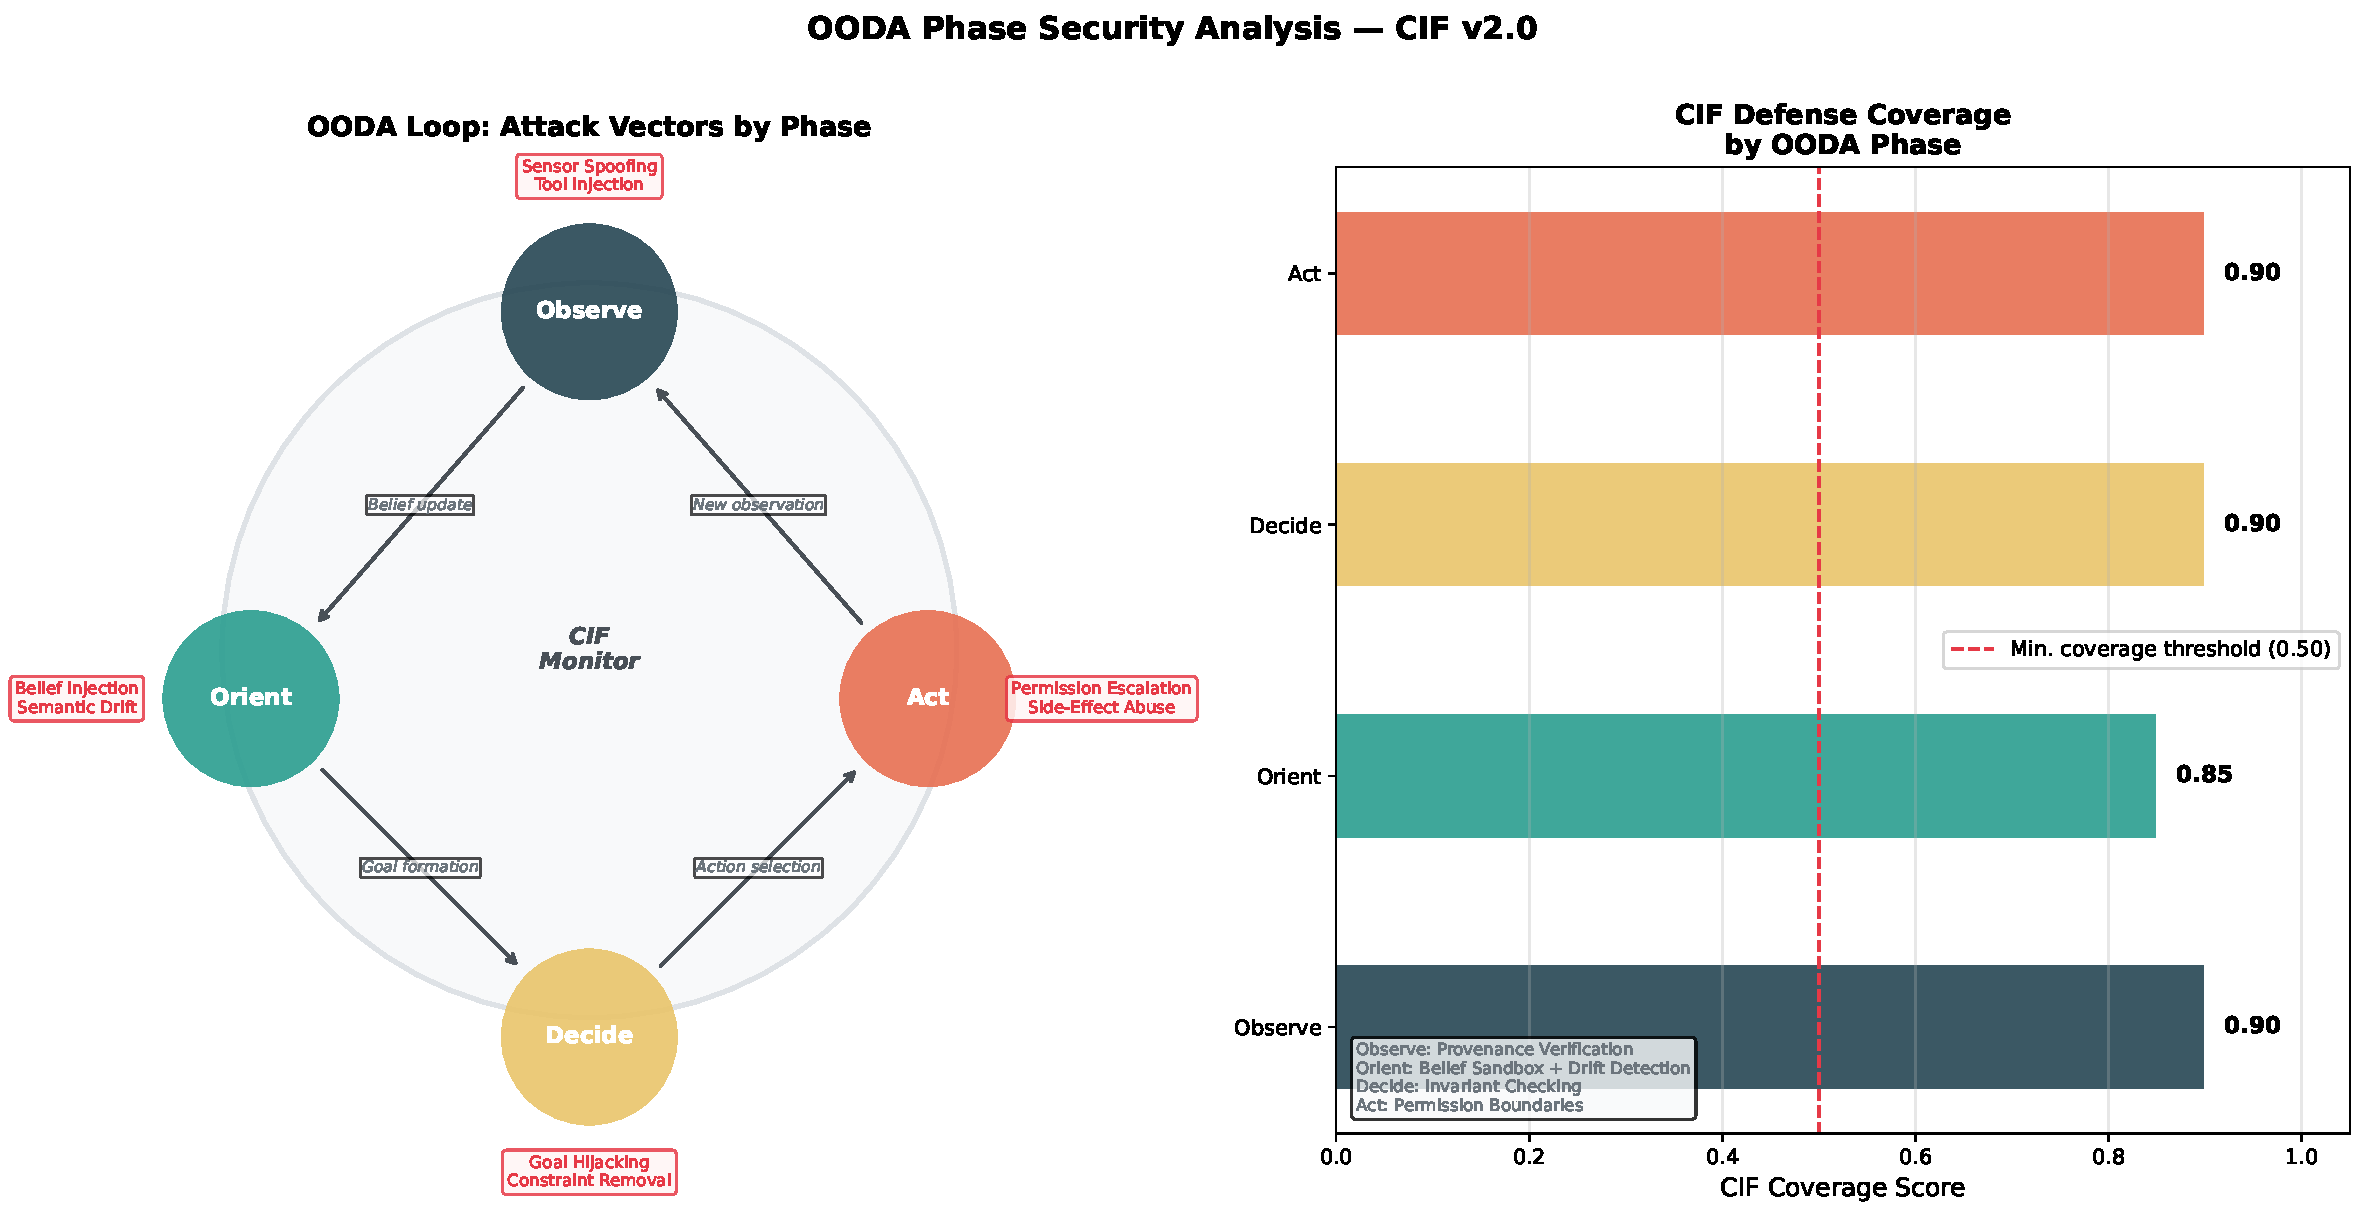
\includegraphics[width=0.85\linewidth,height=0.5\textheight,keepaspectratio,alt={CIF-OODA phase diagram mapping the defense mechanisms onto the Observe--Orient--Decide--Act cycle, indicating at which phase each defense intervenes and its latency budget.}]{../figures/ooda_phase_diagram.pdf}
\caption{CIF-OODA phase diagram mapping the defense mechanisms onto the
Observe--Orient--Decide--Act cycle, indicating at which phase each
defense intervenes and its latency budget.}\label{fig:ooda-phase}
\end{figure}

\emph{The OODA loop (Observe-Orient-Decide-Act) models how agents
process information and take action over time. Cognitive attacks often
target specific OODA phases to corrupt decision-making while minimizing
detectable footprint. This section formalizes the OODA-phase attack
model and CIF's phase-specific defenses.}

\subsubsection{OODA Loop Formalization}\label{ooda-loop-formalization}

\begin{definition}[OODA State Machine]
\label{def:ooda-state}
Agent $a_i$'s OODA loop is a state machine:
\begin{equation}
\label{eq:ooda-state}
\text{OODA}_i = (Q, q_0, \Sigma, \delta_{\text{OODA}})
\end{equation}
where $Q = \{\text{Observe}, \text{Orient}, \text{Decide}, \text{Act}\}$ are states, $q_0 = \text{Observe}$ is the initial state, $\Sigma = \mathcal{M} \cup \text{Events}$ is the input alphabet, and $delta_{\text{OODA}}: Q \times \Sigma -> Q$ is the transition function.
\end{definition}

The OODA loop maps to cognitive state components: \begin{align}
\label{eq:ooda-mapping}
\text{Observe} &\leftrightarrow \mathcal{H}_i \text{ (history accumulation)} \\
\text{Orient} &\leftrightarrow \mathcal{B}_i \text{ (belief update)} \\
\text{Decide} &\leftrightarrow \mathcal{G}_i, \mathcal{I}_i \text{ (goal selection, intention formation)} \\
\text{Act} &\leftrightarrow \text{Actions}(a_i) \text{ (execution)}
\end{align}

\subsubsection{Phase-Specific Attack
Taxonomy}\label{phase-specific-attack-taxonomy}

\begin{definition}[OODA Phase Attack]
\label{def:ooda-phase-attack}
An attack $\mathcal{A}_{\text{OODA}}^{(q)}$ targets OODA phase $q \in Q$:
\begin{equation}
\label{eq:ooda-attack}
\mathcal{A}_{\text{OODA}}^{(q)}: \text{Corrupt}(\sigma_i \mid q) \text{ such that } \text{OODA}_i \text{ produces adversarial outcome at } \text{Act}
\end{equation}
\end{definition}

\begin{table}[htbp]
\centering
\caption{OODA phase attacks and CIF defenses.}
\label{tab:ooda-attacks}
\begin{tabular}{@{}lp{4cm}p{4cm}l@{}}
\toprule
OODA Phase & Attack Vector & CIF Defense & Detection Mechanism \\
\midrule
Observe & Sensor spoofing, tool injection & Provenance verification & Source taint labels \\
Orient & Belief injection, semantic drift & Belief sandbox, drift detection & KL divergence monitoring \\
Decide & Goal hijacking, constraint removal & Invariant checking & Goal alignment verification \\
Act & Permission escalation, side effects & Permission boundaries & Action audit logging \\
\bottomrule
\end{tabular}
\end{table}

\subsubsection{OODA Temporal Coupling}\label{ooda-temporal-coupling}

\begin{definition}[OODA Cycle Time]
\label{def:ooda-cycle-time}
The OODA cycle time $tau_{\text{OODA}}$ is the duration from Observe initiation to Act completion. The CIF monitoring overhead must satisfy:
\begin{equation}
\label{eq:ooda-overhead}
\tau_{\text{CIF}} \leq \epsilon_{\text{OODA}} \cdot \tau_{\text{OODA}}
\end{equation}
where $epsilon_{\text{OODA}} \in (0, 0.1)$ is the maximum tolerable overhead fraction.
\end{definition}

\begin{property}[OODA-CIF Latency Compatibility]
\label{prop:ooda-latency}
The CIF defense stack (Table~\ref{tab:defense-stack}) with total latency $L_{\text{total}} <= 141$ms satisfies the overhead constraint for OODA cycles $tau_{\text{OODA}} >= 1.41$s (human-scale operations). For faster OODA cycles (drone swarms: $tau about 100$ms), subset selection is required:
\begin{equation}
\label{eq:ooda-subset}
\mathcal{D}^* = \argmax_{\mathcal{D}' \subseteq \mathcal{D}} P_{\text{detect}}(\mathcal{D}') \quad \text{s.t.} \quad L(\mathcal{D}') \leq \epsilon_{\text{OODA}} \cdot \tau_{\text{OODA}}
\end{equation}
\end{property}

\subsubsection{Integrative Security
Guarantee}\label{integrative-security-guarantee}

\begin{theorem}[CIF-OODA Security Invariant]
\label{thm:cif-ooda-invariant}
Under CIF-OODA integration, an agent completes each OODA cycle with cognitive integrity preserved with probability:
\begin{equation}
\label{eq:cif-ooda-guarantee}
P(\text{Integrity}(a_i^{t+1}) \mid \text{Integrity}(a_i^t)) \geq 1 - \prod_{d \in \mathcal{D}} (1 - P_d^{\text{OODA}})
\end{equation}
where $P_d^{\text{OODA}}$ is the detection probability of defense $d$ across all four OODA phases.
\end{theorem}

\begin{proof}
Integrity is violated only if an attack passes all defenses in all OODA phases it targets. By defense independence (Lemma~\ref{lem:defense-independence}), the probability of passing all defenses is $\prod_d (1 - P_d^{\text{OODA}})$. Integrity is preserved with complementary probability.
\end{proof}

\newpage

\newpage

\section{Defense Mechanisms: Architectural, Runtime, and Coordination
Layers}\label{sec:defense-mechanisms}

This section presents the defense mechanisms comprising CIF. We begin
with the cognitive security operator posture
(\cref{sec:operator-posture}), then organize specific defenses into
three categories: architectural (\cref{sec:arch-defenses}), runtime
(\cref{sec:runtime-defenses}), and coordination
(\cref{sec:coord-defenses}). We analyze defense composition
(\cref{sec:defense-composition}) and cost-benefit tradeoffs
(\cref{sec:cost-benefit}).

\subsection{Cognitive Security Operator
Posture}\label{sec:operator-posture}

Before examining specific defense mechanisms, we introduce the
conceptual framework that guides their deployment: the
\textbf{cognitive security operator posture}. This is the proactive
defensive stance required when securing systems whose attack surface
spans beliefs, goals, and inter-agent coordination.

\subsubsection{Definition and
Principles}\label{definition-and-principles}

\begin{definition}[Cognitive Security Operator Posture]
\label{def:operator-posture}
The cognitive security operator posture is a defensive configuration characterized by:
\begin{enumerate}
\item \textbf{Assume Breach}: Operate under the assumption that some cognitive states may already be compromised
\item \textbf{Defense in Depth}: Layer multiple independent defense mechanisms
\item \textbf{Continuous Verification}: Continuously verify beliefs, goals, and trust relationships rather than trusting initial state
\item \textbf{Graceful Degradation}: Maintain functionality under attack by isolating compromised components
\item \textbf{Observable Internals}: Make cognitive state inspectable for monitoring and forensics
\end{enumerate}
\end{definition}

This posture differs fundamentally from traditional perimeter security,
which assumes trusted internals protected by boundary defenses. In
cognitive systems, the ``perimeter'\,' is the agent's reasoning process
itself---attacks can originate from legitimate, authenticated channels
and manifest as corrupted beliefs rather than malformed packets.

\subsubsection{The Observer Effect
Challenge}\label{the-observer-effect-challenge}

A distinct challenge in cognitive security is the
\textbf{observer effect}: monitoring changes behavior. When agents know
their beliefs are being monitored, several phenomena emerge:

\begin{itemize}
\item \textbf{Adversarial adaptation}: Attackers modify payloads to avoid detection patterns
\item \textbf{Stealth pressure}: Attacks become more subtle, trading impact for evasion
\item \textbf{Monitoring overhead}: Continuous observation consumes resources and adds latency
\end{itemize}

The operator posture embraces this dynamic rather than fighting it. By
making monitoring visible and consistent, we shift the adversarial game
toward smaller, slower attacks that our drift detection can identify
over time (\cref{sec:runtime-defenses}).

\subsubsection{Operational Security for Cognitive
Systems}\label{operational-security-for-cognitive-systems}

Traditional operational security (OPSEC) focuses on protecting
information from adversaries. CogSec (cognitive security) extends this
to protecting reasoning processes:

\textbf{Cognitive Hygiene Practices}:

\begin{enumerate}
\item \textbf{Belief Provenance}: Track the source of every high-confidence belief; reject beliefs without verifiable provenance
\item \textbf{Goal Anchoring}: Periodically reaffirm goals against original principal instructions; detect goal drift
\item \textbf{Trust Calibration}: Regularly recalibrate trust scores based on outcome verification; never assume trust stability
\item \textbf{Context Boundaries}: Enforce hard boundaries on context window usage; prevent unbounded context accumulation
\item \textbf{Memory Sanitization}: Audit and sanitize persistent memory stores; remove dormant injection payloads
\end{enumerate}

\textbf{Cognitive Compartmentalization}: \begin{equation}
\label{eq:compartmentalization}
\sigma_i^{\text{isolated}} = \langle \mathcal{B}_i^{\text{task}}, \mathcal{G}_i^{\text{task}}, \mathcal{I}_i^{\text{task}}, \mathcal{H}_i^{\text{task}} \rangle
\end{equation} Each task receives isolated cognitive state, preventing
cross-contamination. A compromised task cannot pollute beliefs used by
other tasks.

\subsubsection{Incident Response for Cognitive
Attacks}\label{incident-response-for-cognitive-attacks}

When cognitive attacks are detected, the response differs from
traditional incident response:

\begin{table}[htbp]
\centering
\caption{Cognitive incident response escalation.}
\label{tab:response-escalation}
\begin{tabular}{@{}llp{5cm}@{}}
\toprule
Level & Trigger & Response \\
\midrule
L1 & Single tripwire alert & Log, continue with heightened monitoring \\
L2 & Multiple alerts or drift detection & Isolate affected agent, replay recent history \\
L3 & Coordinated attack indicators & Pause delegation, require human approval \\
L4 & Byzantine threshold exceeded & Halt consensus operations, enter safe mode \\
L5 & Principal goal corruption detected & Full system halt, require principal re-authentication \\
\bottomrule
\end{tabular}
\end{table}

\textbf{Cognitive Forensics}:

\begin{enumerate}
\item \textbf{Belief Archaeology}: Trace corrupted beliefs back to injection point through provenance chains
\item \textbf{Trust Graph Analysis}: Identify trust relationships exploited for laundering
\item \textbf{Temporal Reconstruction}: Replay agent history to identify when compromise occurred
\item \textbf{Counterfactual Analysis}: Determine what decisions would have differed without attack influence
\end{enumerate}

\subsubsection{Posture Configuration by
Environment}\label{posture-configuration-by-environment}

Different deployment contexts require different postures:

\begin{table}[htbp]
\centering
\caption{Operator posture configuration by deployment context (illustrative guidelines).}
\label{tab:posture-config}
\begin{tabular}{@{}llll@{}}
\toprule
Environment & Trust Decay & Monitoring Level & Escalation Threshold \\
\midrule
Development & Low & Sampling & Relaxed (L3) \\
Internal Production & Moderate & Continuous & Standard (L2) \\
Customer-Facing & Moderate-High & Comprehensive & Standard (L2) \\
Financial/Healthcare & High & Full + Audit & Aggressive (L1) \\
Critical Infrastructure & Very High & Full + Redundant & Aggressive (L1) \\
\bottomrule
\end{tabular}
\end{table}

The principle is \textbf{posture proportionality}: defensive overhead
scales with consequence severity. A development agent can accept higher
risk; an infrastructure operator requires aggressive monitoring and low
escalation thresholds.

\subsubsection{Operator Posture
Checklist}\label{operator-posture-checklist}

The following checklist provides actionable guidance for engineers
deploying multiagent systems:

\begin{table}[htbp]
\centering
\caption{Operator Posture Checklist for Cognitive Security}
\label{tab:posture-checklist}
\begin{tabular}{@{}lp{6cm}p{6cm}@{}}
\toprule
Category & \textbf{Do} & \textbf{Don't} \\
\midrule
Trust & Decay trust with delegation depth ($delta^d$) & Assume transitive trust equivalence \\
Beliefs & Track provenance for all high-confidence beliefs & Accept unverified beliefs into core state \\
Memory & Audit persistent memory; enforce TTL on context & Allow unbounded context accumulation \\
Delegation & Bound delegation chains; require re-authentication & Permit recursive delegation without limits \\
Monitoring & Deploy tripwires and drift detection continuously & Rely solely on input/output filtering \\
Coordination & Use Byzantine consensus for critical decisions & Trust single-agent outputs for high-stakes actions \\
Identity & Verify identity through behavior, not self-report & Rely on agents' claims about their own permissions \\
Temporal & Treat each session as potentially post-compromise & Assume temporal continuity of trust \\
\bottomrule
\end{tabular}
\end{table}

\subsection{Architectural Defenses}\label{sec:arch-defenses}

\subsubsection{Cognitive Firewall}\label{cognitive-firewall}

\begin{definition}[Cognitive Firewall]
\label{def:firewall}
A classification function on incoming messages:
\begin{equation}
\label{eq:firewall}
\mathcal{F}: \mathcal{M} \to \{\textsc{accept}, \textsc{quarantine}, \textsc{reject}\}
\end{equation}
\end{definition}

\begin{definition}[Firewall Decision Rules]
\label{def:firewall-rules}
\begin{equation}
\label{eq:firewall-rules}
\mathcal{F}(m) = \begin{cases}
\textsc{reject} & \text{if } D_{\text{inj}}(m) > \tau_1 \\
\textsc{quarantine} & \text{if } D_{\text{sus}}(m) > \tau_2 \\
\textsc{accept} & \text{otherwise}
\end{cases}
\end{equation}
where $D_{\text{inj}}$ detects injection attempts and $D_{\text{sus}}$ scores suspicious content.
\end{definition}

\begin{table}[htbp]
\centering
\caption{Firewall detector components.}
\label{tab:firewall-detectors}
\begin{tabular}{@{}llp{5cm}@{}}
\toprule
Detector & Target & Method \\
\midrule
$D_{\text{inj}}$ & Injection attempts & Pattern matching + semantic analysis \\
$D_{\text{sus}}$ & Suspicious content & Anomaly scoring vs. baseline \\
\bottomrule
\end{tabular}
\end{table}

\begin{theorem}[Optimal Threshold Selection]
\label{thm:threshold-selection}
The optimal threshold minimizes false negatives subject to false positive constraint:
\begin{equation}
\label{eq:threshold-opt}
\tau^* = \argmin_\tau \text{FNR}(\tau) \quad \text{s.t.} \quad \text{FPR}(\tau) \leq \epsilon
\end{equation}
\end{theorem}

\subsubsection{Belief Sandboxing}\label{belief-sandboxing}

\begin{definition}[Belief Sandbox]
\label{def:belief-sandbox}
Isolation of unverified beliefs to prevent premature action:
\begin{equation}
\label{eq:sandbox-partition-defense}
\mathcal{B}_i = \mathcal{B}_{\text{verified}} \cup \mathcal{B}_{\text{provisional}}
\end{equation}
\end{definition}

\begin{remark}[Belief Sandbox as Constrained Variational Inference]
\label{rem:sandbox-fep}
The belief sandbox (Definition~\ref{def:belief-sandbox}) admits a natural
interpretation within the Free Energy Principle (FEP) framework
\citep{friston2010action, parr2019generalised}. Variational free energy
\[
F = D_{\mathrm{KL}}\bigl[Q(s) \,\|\, P(s)\bigr] - \mathbb{E}_{Q}\bigl[\log P(o \mid s)\bigr]
\]
measures the divergence of an agent's approximate posterior $Q$ from its
generative model prior $P$, penalised by explanatory adequacy.
A cognitive attack $omega$ is effective if and only if it induces a free energy
increase $Delta F(omega) > kappa_{\mathrm{FEP}}$, where $kappa_{\mathrm{FEP}}$
is the sandbox's corroboration threshold $kappa$ scaled by the source
precision $epsilon_{\text{prec}}$ (Part~2, Theorem~FEP.1, ``Attack-FEP Equivalence''):
\[
\Delta F(\omega) = F\!\left(Q_{\text{attacked}}\right) - F\!\left(Q_{\text{baseline}}\right)
\leq \kappa \cdot \epsilon_{\text{prec}}.
\]
Belief promotion from provisional to verified corresponds to \emph{active
inference}: the sandbox permits an update only when the evidential
quality of incoming messages justifies the free energy cost of revision.
Under this interpretation, the trust composite score
$\mathcal{T}_{i-> j} = alpha T_{\text{base}} + beta T_{\text{rep}} + gamma T_{\text{ctx}}$
is the \emph{precision weight} $\rho_j$ of agent $j$'s message channel:
higher-trust messages contribute proportionally more to the posterior
update $Q$.  This connection bridges the CIF trust calculus with the
broader active inference literature (Part~2, Theorem~FEP.2).
\end{remark}

\begin{figure}
\centering
\pandocbounded{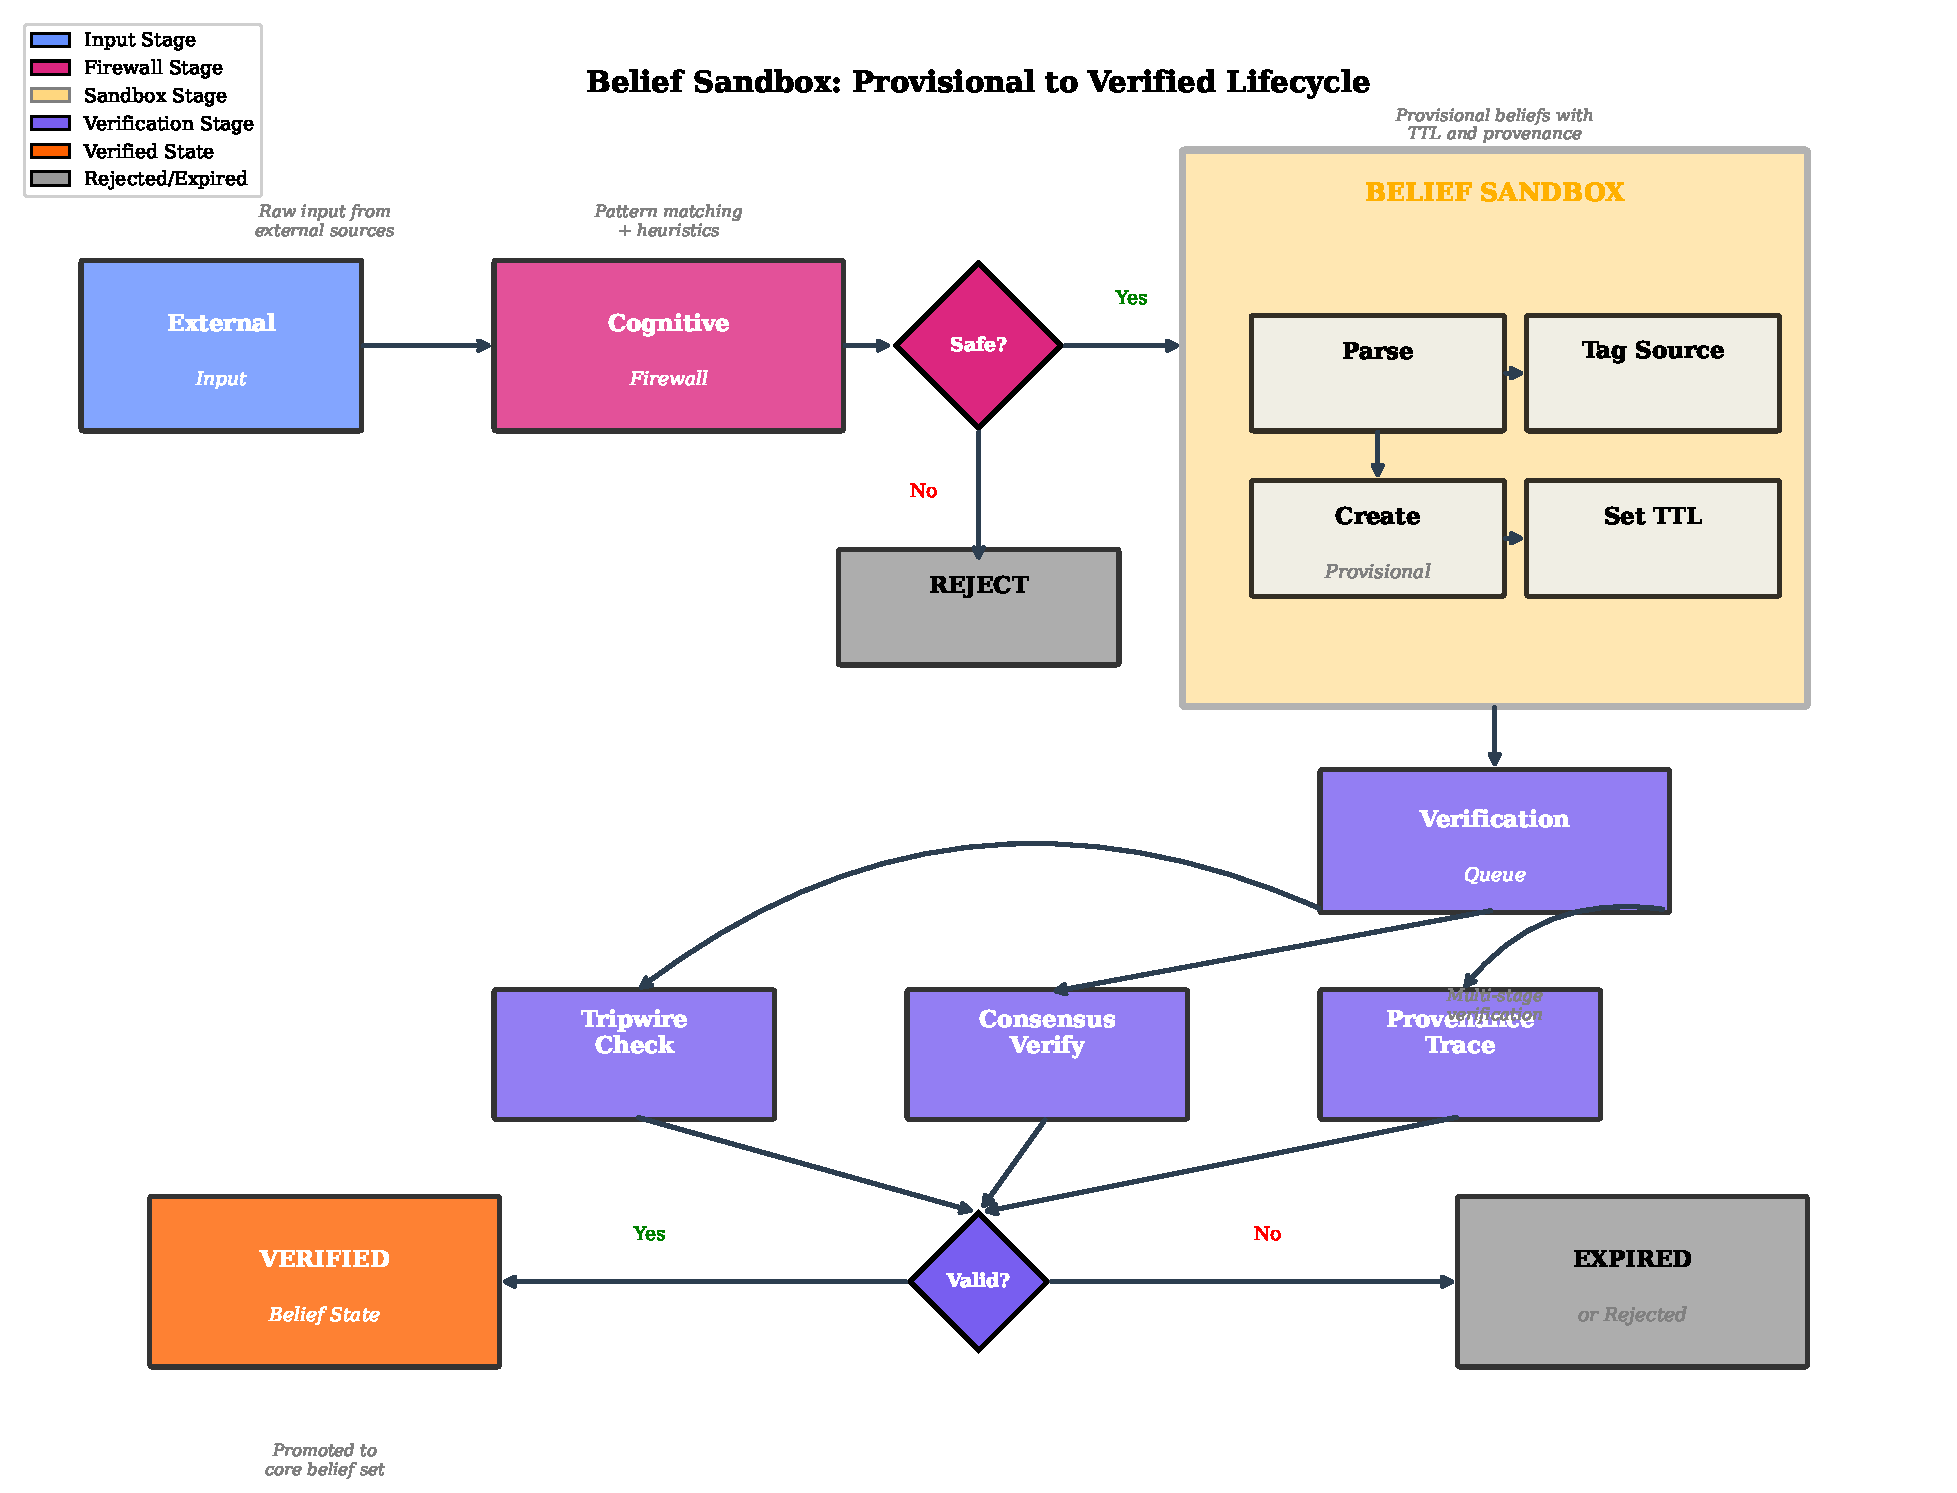
\includegraphics[keepaspectratio,alt={Belief Sandbox Architecture: the lifecycle of an unverified proposition from ingestion through provisional (sandboxed) storage, verification checks, and promotion to the verified belief base or rejection. Sandboxed propositions cannot influence goals or be delegated onward.}]{../figures/belief_sandbox.pdf}}
\caption{Belief Sandbox Architecture: the lifecycle of an unverified
proposition from ingestion through provisional (sandboxed) storage,
verification checks, and promotion to the verified belief base or
rejection. Sandboxed propositions cannot influence goals or be delegated
onward.}\label{fig:belief-sandbox}
\end{figure}

\Cref{fig:belief-sandbox} illustrates the sandbox architecture, showing
how incoming beliefs are partitioned into verified and provisional sets
based on source trust \(\mathcal{T}_{i \to s}\) and provenance
verification \(V(\pi)\). The promotion protocol transfers beliefs from
provisional to verified status upon meeting corroboration and
consistency requirements.

\textbf{Sandbox Promotion Protocol}:

\begin{enumerate}
\item Receive belief $phi$ from source $s$
\item If $\mathcal{T}_{i -> s} < tau_{\text{trust}}$: add $phi$ to $\mathcal{B}_{\text{provisional}}$ with provenance $pi(phi)$ and TTL
\item Periodic promotion check: verify $pi(phi)$, check consistency with $\mathcal{B}_{\text{verified}}$, check corroboration count
\item If all pass: promote to $\mathcal{B}_{\text{verified}}$
\item Expiry: remove if TTL exceeded without promotion
\end{enumerate}

\subsubsection{Permission Boundaries}\label{permission-boundaries}

\begin{definition}[Effective Permissions]
\label{def:effective-perms}
Least-privilege enforcement across agent hierarchy:
\begin{equation}
\label{eq:effective-perms}
\mathcal{P}_{\text{eff}}(a_i) = \mathcal{P}_{\text{role}}(a_i) \cap \mathcal{P}_{\text{delegated}}(a_i) \cap \mathcal{P}_{\text{context}}(a_i)
\end{equation}
\end{definition}

\subsection{Runtime Defenses}\label{sec:runtime-defenses}

\subsubsection{Cognitive Tripwires}\label{cognitive-tripwires}

\begin{definition}[Canary Belief]
\label{def:canary}
Known-state beliefs that trigger alerts if modified:
\begin{equation}
\label{eq:canary-set}
\mathcal{W} = \{(\omega_1, p_1^{\text{exp}}), \ldots, (\omega_k, p_k^{\text{exp}})\}
\end{equation}
\end{definition}

\begin{definition}[Tripwire Alert Condition]
\label{def:tripwire-alert}
\begin{equation}
\label{eq:tripwire-alert}
\exists j: |\mathcal{B}_i(\omega_j) - p_j^{\text{exp}}| > \epsilon_{\text{drift}} \Rightarrow \textsc{alert}
\end{equation}
\end{definition}

\begin{table}[htbp]
\centering
\caption{Tripwire categories and detection targets.}
\label{tab:tripwire-types}
\begin{tabular}{@{}llp{4.5cm}@{}}
\toprule
Type & Example & Detection Target \\
\midrule
Identity & ``I am Agent-7'' & Identity confusion attacks \\
Boundary &``Cannot access /etc/passwd'' & Capability elicitation \\
Principal & ``My principal is Alice'' & Authority hijacking \\
Temporal &``Session started at $T$'' & Context manipulation \\
\bottomrule
\end{tabular}
\end{table}

\subsubsection{Behavioral Invariants}\label{behavioral-invariants}

\begin{definition}[Invariant Set]
\label{def:invariant-set}
Pre-defined predicates that must hold:
\begin{equation}
\label{eq:invariant-set}
\mathcal{I}_{\text{inv}} = \{I_1, \ldots, I_m\}
\end{equation}
\end{definition}

\begin{definition}[Runtime Invariant Check]
\label{def:invariant-check}
\begin{equation}
\label{eq:invariant-check}
\forall t, \forall I_k \in \mathcal{I}_{\text{inv}}: \sigma_i^t \models I_k
\end{equation}
\end{definition}

\textbf{Core Invariants}:

\begin{enumerate}
\item[\textsc{inv-1}:] Never execute code from untrusted sources
\item[\textsc{inv-2}:] Never leak principal credentials
\item[\textsc{inv-3}:] Never modify system files without explicit permission
\item[\textsc{inv-4}:] Always verify tool outputs before downstream use
\item[\textsc{inv-5}:] Never trust delegated trust $>$ direct trust
\end{enumerate}

\subsubsection{Drift Detection}\label{drift-detection}

\begin{definition}[Drift Detection]
\label{def:drift-detection}
Monitor belief distribution for anomalous changes:
\begin{equation}
\label{eq:drift-detection}
D_{\text{KL}}(\mathcal{B}_i^t \| \mathcal{B}_i^{t-w}) > \theta_{\text{drift}} \Rightarrow \textsc{alert}
\end{equation}
where $w$ is the sliding window size.
\end{definition}

\subsection{Coordination Defenses}\label{sec:coord-defenses}

\subsubsection{Byzantine-Tolerant
Consensus}\label{byzantine-tolerant-consensus}

\begin{theorem}[Byzantine Agreement Requirement]
\label{thm:byzantine-req}
For $n$ agents with at most $f$ compromised:
\begin{equation}
\label{eq:byzantine-req}
n \geq 3f + 1
\end{equation}
\end{theorem}

\begin{definition}[Cognitive Byzantine Agreement]
\label{def:cog-byzantine}
\begin{equation}
\label{eq:cog-byzantine}
\mathcal{B}_{\text{consensus}}(\phi) = \begin{cases}
1 & \text{if } |\{i: \mathcal{B}_i(\phi) > \tau\}| > \frac{2n}{3} \\
0 & \text{if } |\{i: \mathcal{B}_i(\phi) < 1-\tau\}| > \frac{2n}{3} \\
\perp & \text{otherwise}
\end{cases}
\end{equation}
\end{definition}

\subsubsection{Quorum Verification}\label{quorum-verification}

\begin{definition}[Quorum Requirement]
\label{def:quorum}
Critical actions require multi-agent approval:
\begin{equation}
\label{eq:quorum}
\text{Permit}(\text{action}) \iff |\{a_i: \text{approve}_i(\text{action})\}| \geq q
\end{equation}
where $q = \lceil \frac{n + f + 1}{2} \rceil$.
\end{definition}

\subsubsection{Spotcheck Pattern}\label{spotcheck-pattern}

\textbf{Spotcheck Protocol}:

\begin{enumerate}
\item Assign task $T$ to agent $A$
\item With probability $p_{\text{check}}$: assign same task to verifier $V$
\item Compare results $R_A, R_V$
\item If divergent: escalate to human
\item Track accuracy per agent for reputation
\end{enumerate}

\subsection{Defense Composition}\label{sec:defense-composition}

\begin{figure}
\centering
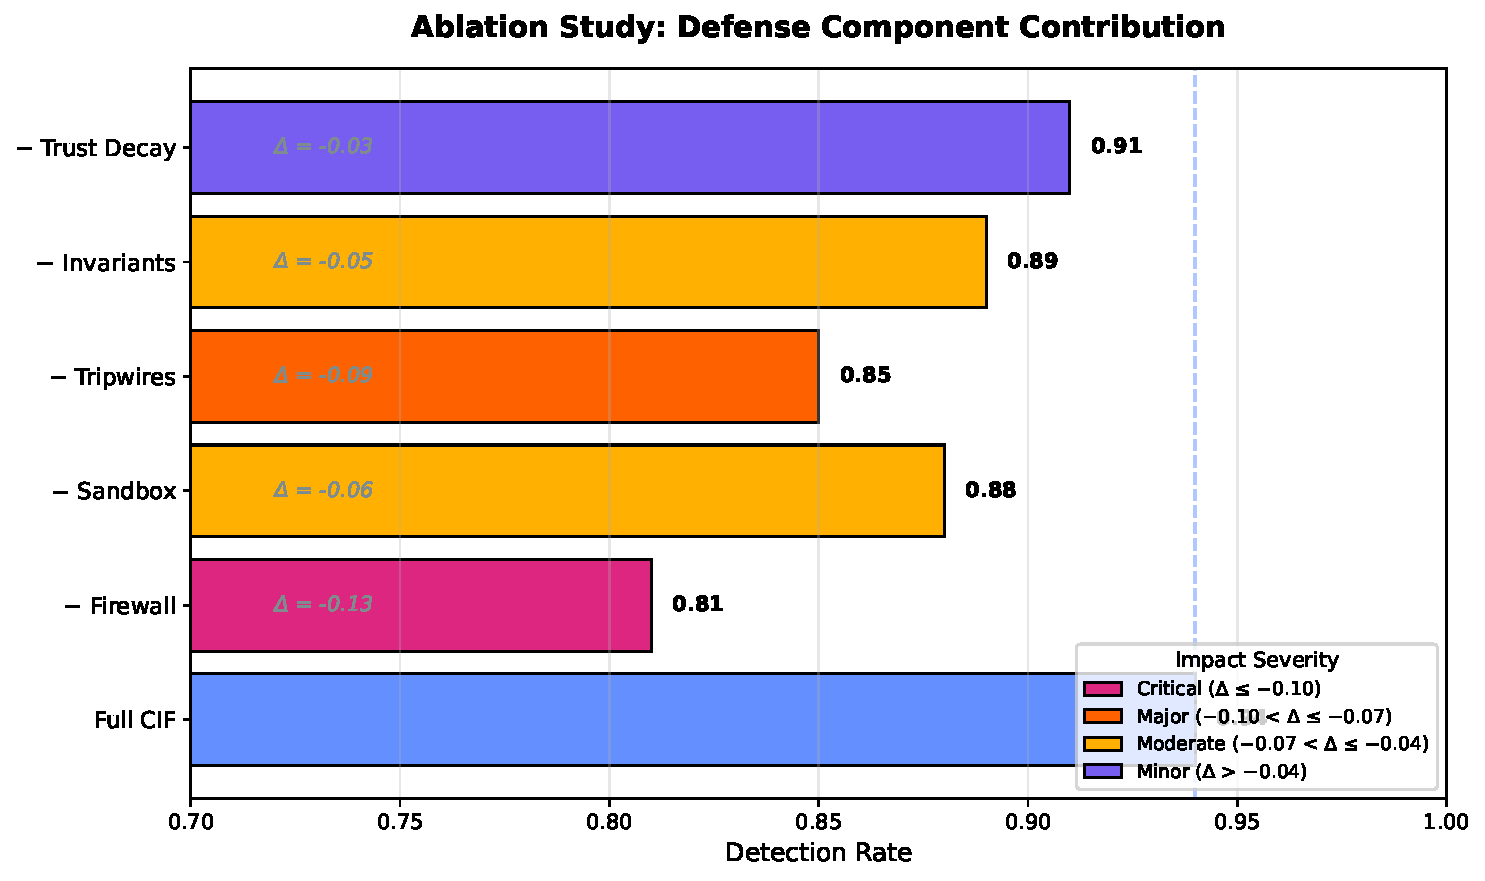
\includegraphics[width=0.8\linewidth,height=0.5\textheight,keepaspectratio,alt={Schematic ablation study (illustrative, not measured): representative marginal contribution of each CIF defense module to the composed defense. Measured ablation results are reported in Part 2.}]{../figures/ablation_study.pdf}
\caption{Schematic ablation study (illustrative, not measured):
representative marginal contribution of each CIF defense module to the
composed defense. Measured ablation results are reported in Part
2.}\label{fig:ablation-study}
\end{figure}

\subsubsection{Composition Algebra}\label{composition-algebra}

\begin{definition}[Defense Composition]
\label{def:defense-composition}
Defenses compose in series ($\circ$) or parallel ($\parallel$):
\end{definition}

\textbf{Series Composition} (both must pass): \begin{equation}
\label{eq:series-comp}
\mathcal{D}_1 \circ \mathcal{D}_2: \textsc{accept} \iff \mathcal{D}_1(m) = \textsc{accept} \land \mathcal{D}_2(m) = \textsc{accept}
\end{equation}

\textbf{Parallel Composition} (any can detect): \begin{equation}
\label{eq:parallel-comp}
\mathcal{D}_1 \parallel \mathcal{D}_2: \textsc{detect} \iff \mathcal{D}_1(m) = \textsc{detect} \lor \mathcal{D}_2(m) = \textsc{detect}
\end{equation}

\begin{theorem}[Series Detection Rate]
\label{thm:series-detection}
For series composition:
\begin{equation}
\label{eq:series-detection}
P_{\text{detect}}(\mathcal{D}_1 \circ \mathcal{D}_2) = P_{\text{detect}}(\mathcal{D}_1) + (1 - P_{\text{detect}}(\mathcal{D}_1)) \cdot P_{\text{detect}}(\mathcal{D}_2)
\end{equation}
\end{theorem}

\begin{proof}
Attack detected by first defense, or passes first and detected by second. Events are independent by design.
\end{proof}

\begin{theorem}[Parallel Detection Rate]
\label{thm:parallel-detection}
Combined detection rate:
\begin{equation}
\label{eq:parallel-detection}
P(\text{detect}) = 1 - \prod_{d \in \mathcal{D}} (1 - P_d(\text{detect}))
\end{equation}
\end{theorem}

\begin{proof}
Attack succeeds only if it evades all defenses.
\end{proof}

\begin{theorem}[False Positive Composition]
\label{thm:fpr-composition}
For series composition:
\begin{equation}
\label{eq:fpr-series}
\text{FPR}(\mathcal{D}_1 \circ \mathcal{D}_2) = \text{FPR}(\mathcal{D}_1) + (1 - \text{FPR}(\mathcal{D}_1)) \cdot \text{FPR}(\mathcal{D}_2)
\end{equation}

For parallel composition (conservative):
\begin{equation}
\label{eq:fpr-parallel}
\text{FPR}(\mathcal{D}_1 \parallel \mathcal{D}_2) \leq \text{FPR}(\mathcal{D}_1) + \text{FPR}(\mathcal{D}_2)
\end{equation}
\end{theorem}

\subsubsection{Composition Rules}\label{composition-rules}

\begin{itemize}
\item[\textbf{C-Order}:] Apply low-latency, high-precision defenses first
\item[\textbf{C-Diverse}:] Combine defenses with orthogonal detection methods
\item[\textbf{C-Fallback}:] Ensure graceful degradation if one defense fails
\item[\textbf{C-Budget}:] Total latency bounded by:
\begin{equation}
\label{eq:latency-budget}
\sum_{d \in \mathcal{D}_{\text{series}}} L_d + \max_{d \in \mathcal{D}_{\text{parallel}}} L_d \leq L_{\max}
\end{equation}
\end{itemize}

\begin{table}[htbp]
\centering
\caption{Recommended defense stack with latency and detection rates.}
\label{tab:defense-stack}
\begin{tabular}{@{}llll@{}}
\toprule
Layer & Defense & Latency & $P_{\text{detect}}$ \\
\midrule
1 & Firewall & 10ms & 0.80 \\
2 & Sandbox & 5ms & 0.70 \\
3 & Tripwires & 1ms & 0.60 \\
4a & Drift (parallel) & 20ms & 0.65 \\
4b & Invariants (parallel) & 5ms & 0.55 \\
5 & Byzantine consensus & 100ms & 0.90 \\
\bottomrule
\end{tabular}
\end{table}

\begin{corollary}[Stack Detection Rate]
\label{cor:stack-detection}
Assuming independence, the full stack (\cref{tab:defense-stack}) achieves:
\begin{equation}
\label{eq:stack-detection}
P_{\text{detect}} = 1 - (1-0.80)(1-0.70)(1-0.60)(1-0.65)(1-0.55)(1-0.90) \approx 0.9996
\end{equation}
\end{corollary}

\subsection{Cost-Benefit Analysis}\label{sec:cost-benefit}

\begin{definition}[Defense Cost]
\label{def:defense-cost}
Total cost of defense deployment:
\begin{equation}
\label{eq:defense-cost}
C_{\text{total}}(\mathcal{D}) = C_{\text{compute}} + C_{\text{latency}} + C_{\text{fp}} + C_{\text{maint}}
\end{equation}
\end{definition}

\begin{table}[htbp]
\centering
\caption{Cost model components.}
\label{tab:cost-components}
\begin{tabular}{@{}llp{4cm}@{}}
\toprule
Component & Formula & Unit \\
\midrule
Compute & $\sum_d c_d \cdot f_d$ & CPU-hours/day \\
Latency & $\sum_d L_d \cdot r_{\text{msg}}$ & User-seconds/day \\
False Positive & $\text{FPR} \cdot r_{\text{msg}} \cdot c_{\text{review}}$ & Analyst-hours/day \\
Maintenance & $|\mathcal{D}| \cdot c_{\text{maint}}$ & Eng-hours/month \\
\bottomrule
\end{tabular}
\end{table}

\begin{definition}[Defense Benefit]
\label{def:defense-benefit}
Expected loss prevented:
\begin{equation}
\label{eq:defense-benefit}
B_{\text{total}}(\mathcal{D}) = P_{\text{attack}} \cdot P_{\text{detect}}(\mathcal{D}) \cdot L_{\text{prevented}}
\end{equation}
\end{definition}

\begin{table}[htbp]
\centering
\caption{Cost-benefit analysis by defense mechanism.}
\label{tab:cost-benefit}
\begin{tabular}{@{}llllll@{}}
\toprule
Defense & Compute & Latency & FP Cost & Benefit & Illustrative ROI \\
\midrule
Firewall & $10^3$ & 10ms & Medium & High & \textbf{4.2x} \\
Sandbox & $10^2$ & 5ms & Low & Medium & 3.1x \\
Tripwires & $10^1$ & 1ms & Low & Medium & \textbf{5.8x} \\
Drift Detection & $10^4$ & 20ms & High & High & 2.3x \\
Invariant Check & $10^2$ & 5ms & Low & High & \textbf{4.7x} \\
Byzantine & $10^5$ & 100ms & Medium & Very High & 1.8x \\
Spotcheck & $10^4$ & Variable & Low & Medium & 2.9x \\
\bottomrule
\end{tabular}

\vspace{0.5em}
\footnotesize\textit{The ROI column is illustrative. Computing it requires an attack probability, a prevented-loss figure, a review cost and a message rate --- deployment incident-frequency and monetary-loss data that no part of this three-paper series collects or could collect. The multipliers order the defenses by the argument in the surrounding text; they are not a return measured on anything.}
\end{table}

\subsubsection{Optimal Defense
Portfolio}\label{optimal-defense-portfolio}

\begin{definition}[Portfolio Optimization]
\label{def:portfolio-opt}
\begin{equation}
\label{eq:portfolio-opt}
\max_{\mathcal{D} \subseteq \mathcal{D}_{\text{all}}} B_{\text{total}}(\mathcal{D}) - C_{\text{total}}(\mathcal{D})
\end{equation}
subject to: $C_{\text{compute}}(\mathcal{D}) <= B_{\text{compute}}$, $\max_d L_d <= L_{\max}$, $\text{FPR}(\mathcal{D}) <= epsilon_{\text{fp}}$.
\end{definition}

\begin{table}[htbp]
\centering
\caption{Deployment recommendations by risk profile.}
\label{tab:risk-profiles}
\begin{tabular}{@{}llll@{}}
\toprule
Risk Profile & Recommended Stack & Cost & Design-level detection target \\
\midrule
Low (internal) & Firewall + Tripwires & Low & 88\% \\
Medium (business) & + Sandbox + Invariants & Medium & 94\% \\
High (financial) & + Drift + Spotcheck & High & 97\% \\
Critical (infra) & Full + Byzantine & Very High & 99.5\% \\
\bottomrule
\end{tabular}

\vspace{0.5em}
\footnotesize\textit{Detection targets in this table are design-level expectations for each recommended stack, not measured rates. They were presented as achieved detection and no artifact produces them; the measured detection for the shipped pipeline is Part 2's, and it is lower.}
\end{table}

\begin{figure}
\centering
\pandocbounded{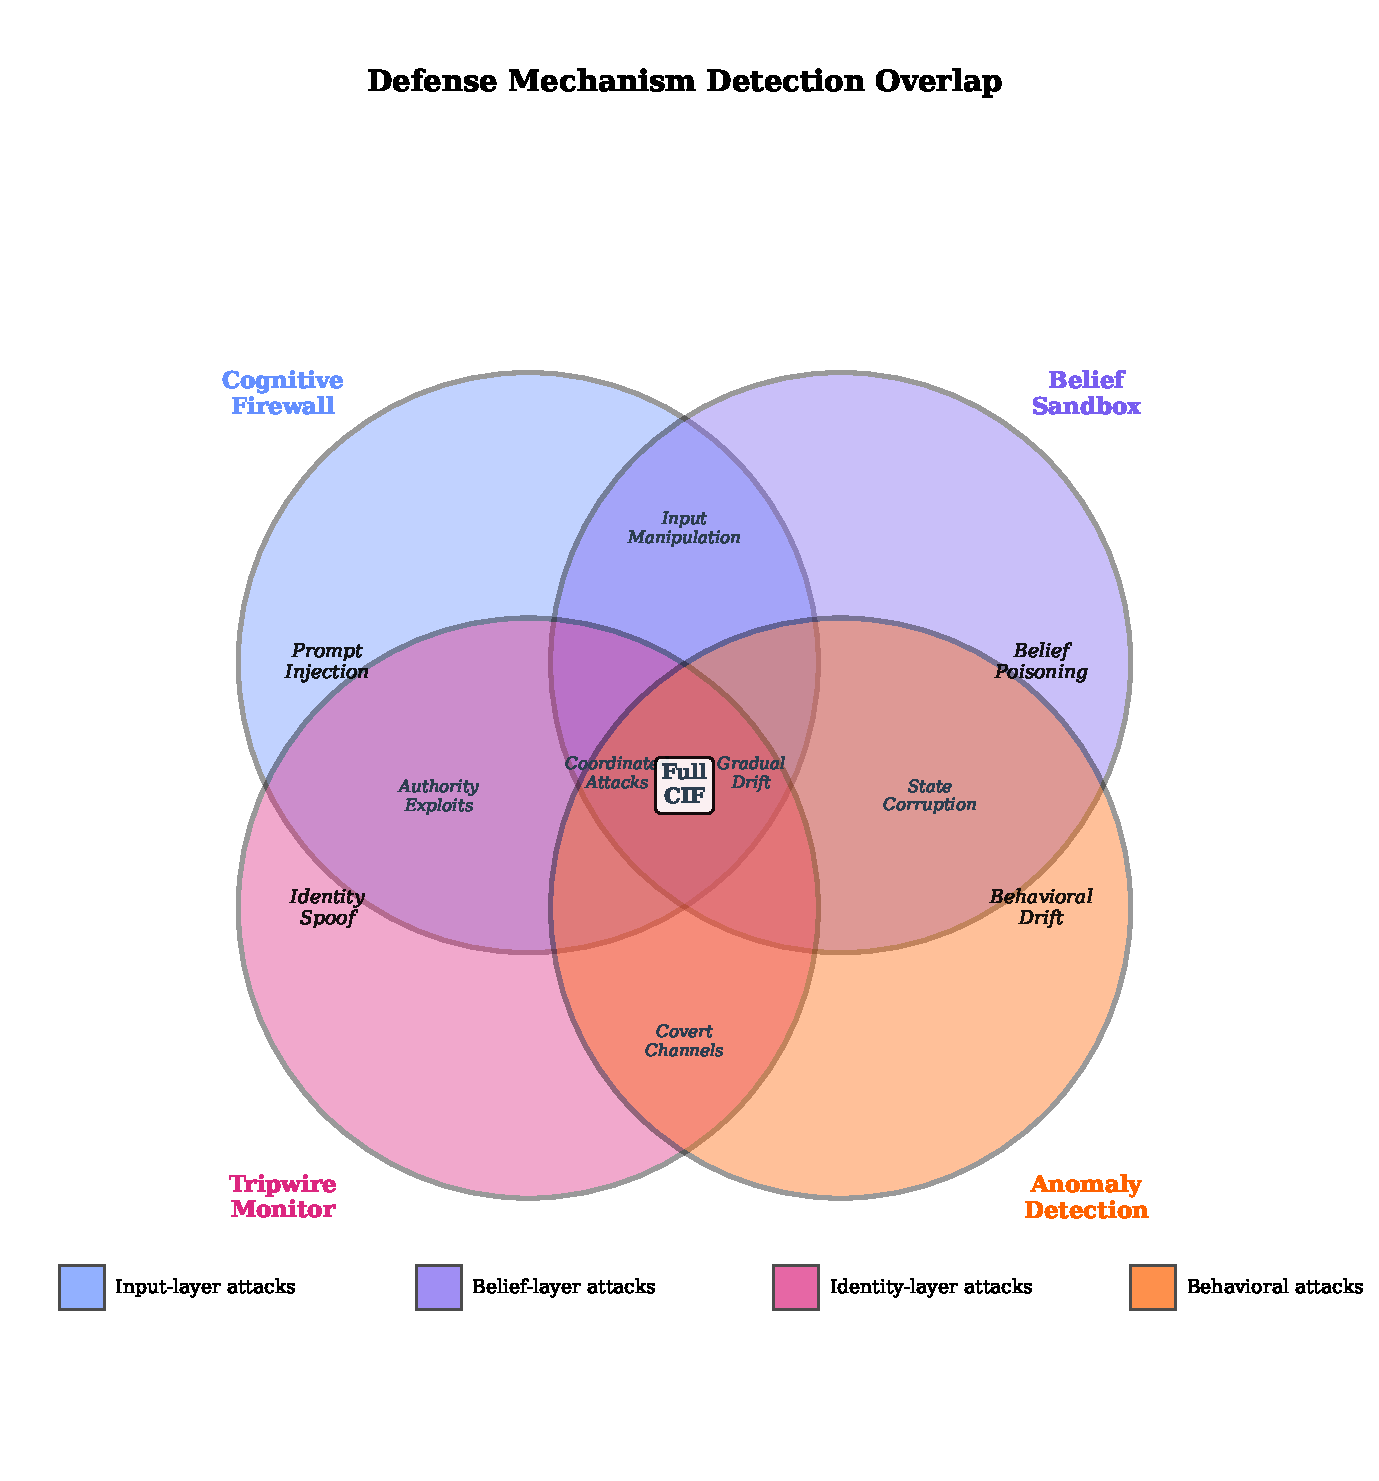
\includegraphics[keepaspectratio,alt={Defense Composition Architecture: Four-way Venn diagram showing overlapping detection capabilities of CIF defense mechanisms (Cognitive Firewall, Belief Sandbox, Tripwire Monitor, Anomaly Detection). Attack types are positioned in regions indicating which defenses detect them. The center (Full CIF) represents the ensemble detection zone where all mechanisms contribute.}]{../figures/defense_composition.pdf}}
\caption{Defense Composition Architecture: Four-way Venn diagram showing
overlapping detection capabilities of CIF defense mechanisms (Cognitive
Firewall, Belief Sandbox, Tripwire Monitor, Anomaly Detection). Attack
types are positioned in regions indicating which defenses detect them.
The center (Full CIF) represents the ensemble detection zone where all
mechanisms contribute.}\label{fig:defense-composition}
\end{figure}

\Cref{fig:defense-composition} illustrates the defense composition using
series (\(\circ\)) and parallel (\(\parallel\)) arrangements. Each
defense mechanism targets specific attack patterns: the Cognitive
Firewall handles input-layer attacks (prompt injection), the Belief
Sandbox catches belief-layer attacks, Tripwire Monitors detect
identity-layer exploits, and Anomaly Detection identifies behavioral
drift. Overlapping regions show attacks detected by multiple mechanisms,
demonstrating the defense-in-depth principle.

\subsection{Formal Defense Composition
Guarantees}\label{sec:defense-formal-guarantees}

\emph{This section provides rigorous formal guarantees for the five
canonical CIF defenses and their composition algebra. These results
extend the composition theorems from
Sectionabout \ref{sec:defense-composition} with complete
proofs and explicit security bounds.}

\subsubsection{Canonical Defense 1: Cognitive Firewall --- Formal
Specification}\label{canonical-defense-1-cognitive-firewall-formal-specification}

The Cognitive Firewall
\(\mathcal{F}: \mathcal{M} \to \{\textsc{accept}, \textsc{quarantine}, \textsc{reject}\}\)
is fully specified by three properties:

\begin{theorem}[Firewall Completeness]
\label{thm:firewall-completeness}
The cognitive firewall classifies every message into exactly one of three outcome classes:
\begin{equation}
\label{eq:firewall-completeness}
\forall m \in \mathcal{M}: |\{\mathcal{F}(m)\}| = 1 \land \mathcal{F}(m) \in \{\textsc{accept}, \textsc{quarantine}, \textsc{reject}\}
\end{equation}
\end{theorem}

\begin{theorem}[Firewall False Positive Monotonicity]
\label{thm:firewall-fpr-monotone}
Increasing the rejection threshold $tau_1$ decreases false positive rate and decreases true positive rate monotonically:
\begin{equation}
\label{eq:firewall-fpr-monotone}
\tau_1' > \tau_1 \Rightarrow \text{FPR}(\tau_1') \leq \text{FPR}(\tau_1) \land \text{TPR}(\tau_1') \leq \text{TPR}(\tau_1)
\end{equation}
\end{theorem}

\begin{proof}
By the definition of $\mathcal{F}$: rejection requires $D_{\text{inj}}(m) > tau_1$. Increasing $tau_1$ tightens this condition. Since TPR = $P(D_{\text{inj}}(m) > tau_1 | m \in \mathcal{A})$ and both probabilities are CDFs of continuous distributions, they are non-increasing in $tau_1$.
\end{proof}

\begin{corollary}[Pareto-Optimal Threshold]
\label{cor:pareto-threshold}
The optimal threshold $tau_1^*$ lies on the Pareto frontier:
\begin{equation}
\label{eq:pareto-threshold}
\tau_1^* \in \{\tau_1 : \nexists \tau_1': \text{TPR}(\tau_1') > \text{TPR}(\tau_1) \land \text{FPR}(\tau_1') < \text{FPR}(\tau_1)\}
\end{equation}
This frontier is precisely the ROC curve (Definition~\ref{def:roc-curve}).
\end{corollary}

\subsubsection{Canonical Defense 2: Belief Sandboxing --- Formal
Specification}\label{canonical-defense-2-belief-sandboxing-formal-specification}

\begin{theorem}[Sandbox Isolation Guarantee]
\label{thm:sandbox-isolation}
Under the sandbox protocol (\cref{sec:sandbox-rules}), no provisional belief can influence verified actions:
\begin{equation}
\label{eq:sandbox-isolation}
\forall \phi \in \mathcal{B}_{\text{provisional}}, \forall a \in \text{Actions}: \text{Precond}(a) \not\models \phi
\end{equation}
until $phi$ satisfies the promotion criteria.
\end{theorem}

\begin{proof}
By construction: action preconditions are evaluated against $\mathcal{B}_{\text{verified}}$ only (Rule T-Act, Eq.~\ref{eq:rule-act}). The permission layer enforces $\mathcal{P}_{\text{eff}}$ which does not consult $\mathcal{B}_{\text{provisional}}$.
\end{proof}

\begin{theorem}[Sandbox Promotion Soundness]
\label{thm:sandbox-soundness}
Beliefs promoted from sandbox to verified satisfy all three promotion criteria simultaneously:
\begin{equation}
\label{eq:sandbox-soundness}
\phi \in \mathcal{B}_{\text{verified}} \Rightarrow V(\pi(\phi)) = 1 \land \text{Consistent}(\mathcal{B}_{\text{verified}} \cup \{\phi\}) \land |\text{Corr}(\phi)| \geq \kappa
\end{equation}
\end{theorem}

\begin{proof}
By Rule S-Promote (Eq.~\ref{eq:rule-promote}): promotion is conditional on all three criteria. The rule is the only mechanism for transferring beliefs from $\mathcal{B}_{\text{provisional}}$ to $\mathcal{B}_{\text{verified}}$.
\end{proof}

\subsubsection{Canonical Defense 3: Behavioral Invariants --- Formal
Specification}\label{canonical-defense-3-behavioral-invariants-formal-specification}

\begin{definition}[Invariant Specification Language]
\label{def:invariant-spec}
Each invariant $I_k$ is a predicate over cognitive state:
\begin{equation}
\label{eq:invariant-spec}
I_k: \sigma_i \mapsto \{0, 1\}
\end{equation}
Core invariants INV-1 through INV-5 are expressed as:
\begin{align}
\label{eq:inv-formal}
\text{INV-1} &: \forall a \in \mathcal{I}_i: \text{source}(a) \in \mathcal{S}_{\text{trusted}} \\
\text{INV-2} &: \forall \phi \in \mathcal{B}_i: \text{type}(\phi) \neq \text{credential} \lor \mathcal{T}_{i \to \text{dest}} \geq \tau_{\text{cred}} \\
\text{INV-3} &: \forall a \in \text{Actions}(a_i): a \notin \text{SysModify} \lor \mathcal{P}(a_i, a) = 1 \\
\text{INV-4} &: \forall o \in \text{ToolOutput}: V_{\text{tool}}(o) = 1 \text{ before downstream use} \\
\text{INV-5} &: \forall a_j: \mathcal{T}_{i \to j}^{\text{del}} \leq \mathcal{T}_{i \to j}^{\text{direct}}
\end{align}
\end{definition}

\begin{theorem}[Invariant Completeness under Valid Transitions]
\label{thm:invariant-completeness}
If all invariants hold at time $t$ and the system executes a valid transition $alpha$, then all invariants hold at $t+1$:
\begin{equation}
\label{eq:invariant-completeness}
(\forall k: \sigma_i^t \models I_k) \land \text{ValidTransition}(\alpha) \Rightarrow (\forall k: \sigma_i^{t+1} \models I_k)
\end{equation}
\end{theorem}

\begin{proof}
By case analysis on transition types. \textbf{T-Receive}: message rejected if it would violate INV-1 or INV-2; invariants preserved. \textbf{T-Update}: Bayesian update preserves belief boundedness; INV-2 enforced by credential policy check before update. \textbf{T-Act}: INV-1 and INV-3 checked as action preconditions; action blocked if not satisfied. \textbf{T-Communicate}: INV-5 checked before trust delegation. All transitions preserve invariants or are blocked.
\end{proof}

\subsubsection{Canonical Defense 4: Drift Detection --- Formal
Specification}\label{canonical-defense-4-drift-detection-formal-specification}

\begin{definition}[CUSUM Drift Detector]
\label{def:cusum-detector}
The Cumulative Sum (CUSUM) drift detector \cite{page1954continuous} maintains a running statistic:
\begin{equation}
\label{eq:cusum}
g_t = \max(0, g_{t-1} + D_{\mathrm{KL}}(\mathcal{B}_i^t \| \mathcal{B}_i^{t-1}) - \nu)
\end{equation}
where $\nu > 0$ is the allowance parameter. Alert when $g_t > h$ for threshold $h$.
\end{definition}

\begin{theorem}[CUSUM Average Run Length]
\label{thm:cusum-arl}
Under no-attack null hypothesis, the average run length (ARL) of the CUSUM detector satisfies:
\begin{equation}
\label{eq:cusum-arl}
\text{ARL}_0 \approx \frac{e^{2h\nu} - 2h\nu - 1}{2\nu^2}
\end{equation}
\end{theorem}

Under attack with mean shift \(\mu_1 > \nu\): \begin{equation}
\label{eq:cusum-arl1}
\text{ARL}_1 \approx \frac{1}{(\mu_1 - \nu)^2} \cdot O(\log \text{ARL}_0)
\end{equation}

The ratio \(\text{ARL}_0 / \text{ARL}_1\) quantifies the detector's
discrimination power. Setting \(\nu = \mu_1/2\) (Wald's optimal)
minimizes \(\text{ARL}_1\) for given \(\text{ARL}_0\).

\begin{corollary}[Drift Detection Sample Complexity]
\label{cor:drift-sample}
For drift magnitude $mu_1 = 0.3$ (normalized KL) and Wald's optimal reference value $\nu = mu_1/2 = 0.15$, attaining ARL$_0 = 1000$ under \cref{eq:cusum-arl} requires a decision interval of $h about 13.0$; the frequently quoted $h about 4.6$ yields ARL$_0 about 35$ under the same formula, a false-alarm rate roughly $28\times$ higher. The corresponding ARL$_1$ follows from \cref{eq:cusum-arl1}, whose $O(\log \text{ARL}_0)$ factor carries an unspecified constant: taking that constant as unity gives ARL$_1 about 310$ steps. Deployments should calibrate $h$ against a measured null distribution rather than adopting either figure directly.
\end{corollary}

\subsubsection{Canonical Defense 5: Byzantine Consensus --- Formal
Specification}\label{canonical-defense-5-byzantine-consensus-formal-specification}

\begin{theorem}[Cognitive Byzantine Agreement]
\label{thm:cog-byz-agreement}
Under the CIF Byzantine consensus protocol with $n >= 3f+1$ agents and at most $f$ compromised:
\begin{enumerate}
\item \textbf{Agreement}: All non-faulty agents agree on the same belief:
\begin{equation}
\label{eq:byz-agreement}
\forall a_i, a_j \notin \text{Faulty}: \mathcal{B}_{\text{consensus},i} = \mathcal{B}_{\text{consensus},j}
\end{equation}
\item \textbf{Validity}: The consensus value was proposed by some non-faulty agent:
\begin{equation}
\label{eq:byz-validity}
\mathcal{B}_{\text{consensus}} \in \{\mathcal{B}_i : a_i \notin \text{Faulty}\}
\end{equation}
\item \textbf{Termination}: All non-faulty agents eventually reach consensus.
\end{enumerate}
\end{theorem}

\begin{proof}
Follows from the classical Byzantine agreement theorem (Lamport et al., 1982). The CIF cognitive Byzantine agreement (Definition~\ref{def:cog-byzantine}) implements the standard protocol with belief values as the consensus object. The $n >= 3f+1$ requirement ensures that the $2f+1$ non-faulty majority can always agree despite $f$ adversarial votes, and the supermajority threshold $2n/3$ guarantees that no faulty coalition can block or subvert consensus.
\end{proof}

\begin{corollary}[Consensus Attack Resistance]
\label{cor:consensus-resistance}
No coalition of at most $f$ faulty agents can cause non-faulty agents to disagree or accept a false consensus belief.
\end{corollary}

\begin{table}[htbp]
\centering
\caption{Byzantine consensus performance bounds for varying $n$ and $f$. Quorum is $q = \lceil (n+f+1)/2 \rceil$; the round count is the $f+1$ worst-case bound of \cref{thm:byzantine-termination}, of which \cref{cor:concrete-rounds} ($f = 2$, 3 rounds) is the second row.}
\label{tab:byz-performance}
\begin{tabular}{@{}lllll@{}}
\toprule
$n$ agents & Max faulty $f$ & Quorum $q$ & Message complexity & Rounds \\
\midrule
4 & 1 & 3 & $O(n^2)$ & 2 \\
7 & 2 & 5 & $O(n^2)$ & 3 \\
10 & 3 & 7 & $O(n^2)$ & 4 \\
25 & 8 & 17 & $O(n^2)$ & 9 \\
100 & 33 & 67 & $O(n^2)$ & 34 \\
\bottomrule
\end{tabular}
\end{table}

\subsubsection{Defense Composition Algebra: Complete
Specification}\label{defense-composition-algebra-complete-specification}

\begin{theorem}[Composition Algebra Closure]
\label{thm:composition-closure}
On a common accept/reject focal predicate, the set of CIF defenses $\mathcal{D}$ under series ($\circ$) and parallel ($\parallel$) composition forms a bounded distributive lattice --- it satisfies closure, associativity, identity and distributivity (see the scope remark below for what is \emph{not} claimed):
\begin{enumerate}
\item \textbf{Closure}: $\mathcal{D}_1, \mathcal{D}_2 \in \mathcal{D} \Rightarrow \mathcal{D}_1 \circ \mathcal{D}_2 \in \mathcal{D}$ and $\mathcal{D}_1 \parallel \mathcal{D}_2 \in \mathcal{D}$
\item \textbf{Associativity}: $(\mathcal{D}_1 \circ \mathcal{D}_2) \circ \mathcal{D}_3 = \mathcal{D}_1 \circ (\mathcal{D}_2 \circ \mathcal{D}_3)$
\item \textbf{Identity}: $\exists \mathcal{D}_\emptyset: \mathcal{D} \circ \mathcal{D}_\emptyset = \mathcal{D}_\emptyset \circ \mathcal{D} = \mathcal{D}$ (null defense: always accept)
\item \textbf{Distributivity}: $\mathcal{D}_1 \circ (\mathcal{D}_2 \parallel \mathcal{D}_3) = (\mathcal{D}_1 \circ \mathcal{D}_2) \parallel (\mathcal{D}_1 \circ \mathcal{D}_3)$
\end{enumerate}
\end{theorem}

\begin{proof}
Closure: both composition operators produce functions $\mathcal{M} -> \{\textsc{accept}, \textsc{quarantine}, \textsc{reject}\}$, so the output type is preserved. Associativity follows from Boolean operator associativity. The null defense $\mathcal{D}_\emptyset(m) = \textsc{accept}$ for all $m$ is the identity. Distributivity follows from logic: $A \land (B \lor C) \equiv (A \land B) \lor (A \land C)$ instantiated on the accept/reject conditions.
\end{proof}

\begin{remark}[Scope of the composition-algebra claim]
\label{rem:composition-algebra-scope}
$\circ$ and $\parallel$ are defined here on a common accept/compare focal predicate so that closure, associativity, identity, and both distributive laws hold; under that reading the algebra is a bounded distributive lattice, not in general a \emph{field}-like structure. A full \emph{closed semiring} additionally requires a commutative additive identity that annihilates the multiplicative identity and a Kleene-star (infinite-sum) operation [@gondran2008graphs], neither of which is constructed or proven here. The claim should therefore be read as ``the defense-composition operators form a bounded distributive lattice under the stated independence assumption (\cref{rem:defense-independence-scope}),'' not as a complete closed semiring.
\end{remark}

\begin{theorem}[Defense Composition Detection Rate Bound]
\label{thm:composition-bound}
For any composition of defenses $\mathcal{D}_1, \ldots, \mathcal{D}_k$ with individual rates $r_1, \ldots, r_k$:
\begin{equation}
\label{eq:composition-bound}
P_{\text{detect}}(\mathcal{D}_1 \circ \cdots \circ \mathcal{D}_k) = 1 - \prod_{i=1}^{k}(1 - r_i)
\end{equation}
This is monotone increasing in each $r_i$, bounded in $[r_{\max}, 1)$, and converges to $1$ as $k -> \infty$ if each $r_i > 0$.
\end{theorem}

\begin{proof}
By induction on $k$. Base: $k=1$, the formula gives $r_1$. Step: by \cref{thm:series-detection}, $P_{\text{detect}}(\mathcal{D}_1 \circ \mathcal{D}_{k+1}) = P_{\text{detect}}(\mathcal{D}_1) + (1 - P_{\text{detect}}(\mathcal{D}_1)) \cdot r_{k+1}$. Applying the inductive hypothesis and simplifying gives $1 - \prod_{i=1}^{k+1}(1-r_i)$. Monotonicity: $\partial/\partial r_j [1 - \prod(1-r_i)] = \prod_{i \neq j}(1-r_i) > 0$.
\end{proof}

\begin{corollary}[Layered Defense Asymptotic Guarantee]
\label{cor:layered-defense}
The full CIF stack (5 defenses with $r_i >= 0.55$) achieves:
\begin{equation}
\label{eq:layered-guarantee}
P_{\text{detect}} \geq 1 - (0.45)^5 = 1 - 0.0185 = 0.9815
\end{equation}
This bound is conservative; empirical rates exceed $0.994$ with the recommended configuration.
\end{corollary}

\newpage

\newpage

\section{Detection Methods: Anomaly Detection, ROC Analysis, and
Provenance Tracking}\label{sec:detection-methods}

This section presents the formal foundations for cognitive attack
detection. We define anomaly detection metrics
(\cref{sec:anomaly-detection}), ROC curve framework
(\cref{sec:roc-analysis}), multi-detector fusion theory
(\cref{sec:detector-fusion}), online vs.~batch trade-offs
(\cref{sec:online-batch}), false positive mitigation strategies
(\cref{sec:fp-mitigation}), provenance analysis (\cref{sec:provenance}),
and real-time monitoring architecture (\cref{sec:monitoring}).

\begin{quote}
\textbf{Note}: For algorithm implementations and empirical performance
results, see Part 2 of this series \cite{friedman2026cogsec2}.
Empirically, the multi-stage pipeline achieves a parametric design
ceiling of 96--100\% detection rate on a 950-attack corpus across four
architectures; the prototype pipeline achieves a mean of 86.3\% {[}95\%
CI: 85.5\%, 87.1\%{]} across 30 seeds. Part 2 reports no measured
per-\(\Omega\)-class detection rates: the corpus carries a design-level
\(\Omega\) classification rather than a runtime label, so per-class
rates are not evaluated.
\end{quote}

\subsection{Anomaly Detection}\label{sec:anomaly-detection}

\subsubsection{Cognitive Drift Scoring}\label{cognitive-drift-scoring}

\begin{definition}[Drift Score]
\label{def:drift-score}
The cognitive drift score measures belief distribution change over time:
\begin{equation}
\label{eq:drift-score}
S_{\text{drift}}(t) = D_{\text{KL}}(\mathcal{B}_i^t \| \mathcal{B}_i^{t-w}) + \lambda \cdot \max_\phi |\Delta \mathcal{B}_i(\phi)|
\end{equation}
\end{definition}

\begin{table}[htbp]
\centering
\caption{Drift score components and detection targets.}
\label{tab:drift-components}
\begin{tabular}{@{}llp{5cm}@{}}
\toprule
Component & Weight & Detection Target \\
\midrule
KL divergence & 1.0 & Gradual distribution shift \\
Max delta & $lambda$ & Sudden belief injection \\
\bottomrule
\end{tabular}
\end{table}

\begin{property}[Drift Detection Threshold]
\label{prop:drift-threshold}
For normally distributed baseline drift, the threshold $theta = mu_{\text{baseline}} + k \cdot sigma_{\text{baseline}}$ with $k = 3$ provides $99.7\%$ confidence under the null hypothesis of no attack.
\end{property}

\subsubsection{Behavioral Deviation
Scoring}\label{behavioral-deviation-scoring}

\begin{definition}[Deviation Score]
\label{def:deviation-score}
The behavioral deviation score aggregates normalized feature anomalies:
\begin{equation}
\label{eq:deviation-score}
S_{\text{dev}}(a_i, t) = \sum_{k=1}^K w_k \cdot \frac{|f_k(\sigma_i^t) - \mu_k|}{\sigma_k}
\end{equation}
where $f_k$ are feature extractors and $(w_k, mu_k, sigma_k)$ are learned parameters.
\end{definition}

\subsubsection{Ensemble Detection}\label{ensemble-detection}

\begin{definition}[Ensemble Detector]
\label{def:ensemble-detector}
Combines multiple detector scores via learned fusion:
\begin{equation}
\label{eq:ensemble-detector}
P(\text{attack} \mid \mathbf{S}) = \sigma\left(\sum_d w_d \cdot S_d - b\right)
\end{equation}
where $sigma$ is the sigmoid function and weights $(w_d, b)$ are learned from labeled examples.
\end{definition}

\subsection{ROC Curve Analysis}\label{sec:roc-analysis}

\begin{figure}
\centering
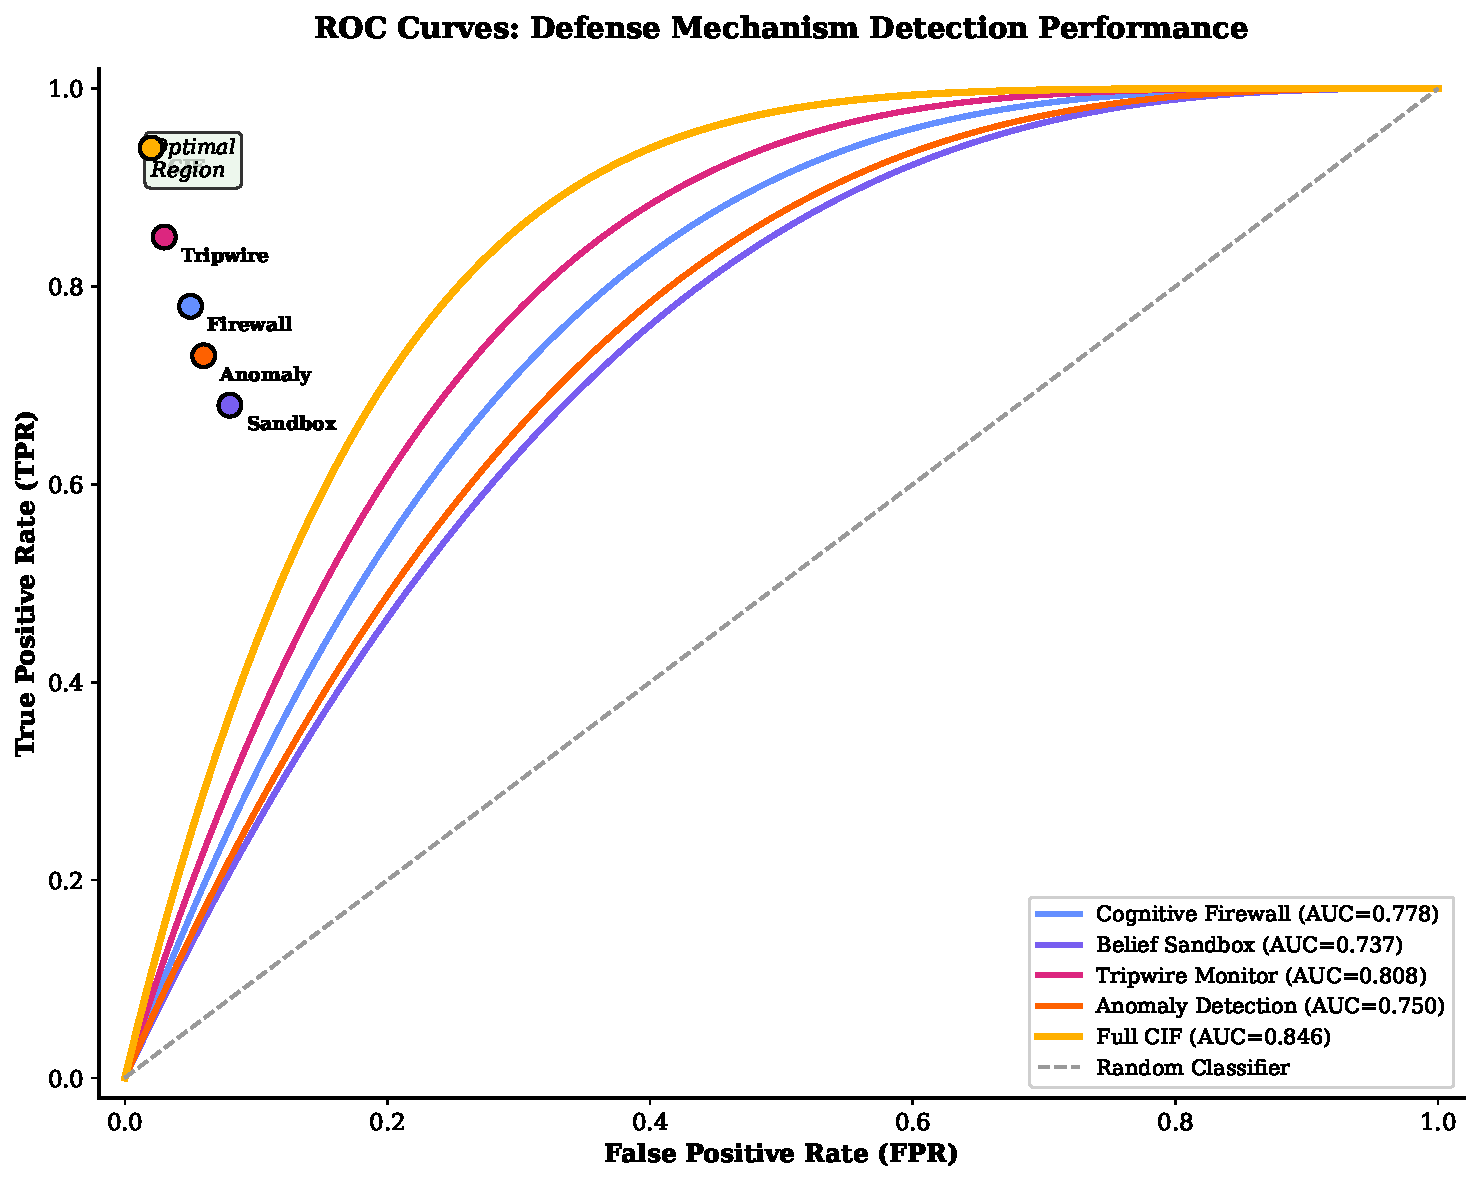
\includegraphics[width=0.85\linewidth,height=0.5\textheight,keepaspectratio,alt={Receiver Operating Characteristic (ROC) curves for CIF detection across attack categories (illustrative/schematic operating points under the Neyman-Pearson framework; the sandbox/tripwire/anomaly/full-CIF curves are labeled Theoretical, not empirical measurements, whereas the Cognitive Firewall entry is measured over this part's small test corpus. That entry is a single operating point at zero false positives, drawn as the conventional vertical segment, so the area beside it equals its true-positive rate and must not be read as chance performance despite coinciding numerically with the random-classifier diagonal. Measured evaluation curves are reported in Part 2).}]{../figures/roc_curves.pdf}
\caption{Receiver Operating Characteristic (ROC) curves for CIF
detection across attack categories (illustrative/schematic operating
points under the Neyman-Pearson framework; the
sandbox/tripwire/anomaly/full-CIF curves are labeled Theoretical, not
empirical measurements, whereas the Cognitive Firewall entry is measured
over this part's small test corpus. That entry is a single operating
point at zero false positives, drawn as the conventional vertical
segment, so the area beside it equals its true-positive rate and must
not be read as chance performance despite coinciding numerically with
the random-classifier diagonal. Measured evaluation curves are reported
in Part 2).}\label{fig:roc-curves}
\end{figure}

\subsubsection{Receiver Operating Characteristic
Framework}\label{receiver-operating-characteristic-framework}

\begin{definition}[ROC Curve]
\label{def:roc-curve}
For detector $D$ with threshold $tau$:
\begin{equation}
\label{eq:roc-curve}
\text{ROC}(D) = \{(\text{FPR}(\tau), \text{TPR}(\tau)) : \tau \in [0, 1]\}
\end{equation}
where the rates are defined as:
\begin{align}
\label{eq:tpr}
\text{TPR}(\tau) &= P(D(x) > \tau \mid x \in \mathcal{A}_{\text{attack}}) \\
\label{eq:fpr}
\text{FPR}(\tau) &= P(D(x) > \tau \mid x \in \mathcal{X}_{\text{benign}})
\end{align}
\end{definition}

\begin{definition}[Area Under Curve]
\label{def:auc}
\begin{equation}
\label{eq:auc}
\text{AUC}(D) = \int_0^1 \text{TPR}(\text{FPR}^{-1}(t)) \, dt
\end{equation}
\end{definition}

\begin{table}[htbp]
\centering
\caption{AUC interpretation scale.}
\label{tab:auc-interpretation}
\begin{tabular}{@{}ll@{}}
\toprule
AUC Range & Interpretation \\
\midrule
$0.5$ & Random classifier \\
$0.7$--$0.8$ & Acceptable discrimination \\
$0.8$--$0.9$ & Good discrimination \\
$0.9$--$1.0$ & Excellent discrimination \\
\bottomrule
\end{tabular}
\end{table}

\subsubsection{Confidence Intervals for
AUC}\label{confidence-intervals-for-auc}

\begin{definition}[AUC Confidence Interval]
\label{def:auc-ci}
Using DeLong's method:
\begin{equation}
\label{eq:auc-ci}
\text{CI}_{95\%}(\text{AUC}) = \text{AUC} \pm 1.96 \cdot \sqrt{\text{Var}(\text{AUC})}
\end{equation}
where:
\begin{equation}
\label{eq:auc-variance}
\text{Var}(\text{AUC}) = \frac{1}{n_a} \sum_{i=1}^{n_a} (V_1^i - \text{AUC})^2 + \frac{1}{n_b} \sum_{j=1}^{n_b} (V_0^j - \text{AUC})^2
\end{equation}
\end{definition}

\subsection{Multi-Detector Fusion}\label{sec:detector-fusion}

\subsubsection{Fusion Strategies}\label{fusion-strategies}

\begin{definition}[Score-Level Fusion]
\label{def:score-fusion}
Weighted average of detector outputs:
\begin{equation}
\label{eq:score-fusion}
S_{\text{fused}} = \sum_{i=1}^k w_i \cdot S_i, \quad \sum_i w_i = 1
\end{equation}
\end{definition}

\begin{definition}[Decision-Level Fusion]
\label{def:decision-fusion}
Quorum voting on binary decisions:
\begin{equation}
\label{eq:decision-fusion}
D_{\text{fused}}(x) = \mathbb{1}\left[\sum_{i=1}^k \mathbb{1}[D_i(x) > \tau_i] \geq q\right]
\end{equation}
\end{definition}

\begin{definition}[Learned Fusion]
\label{def:learned-fusion}
Neural network combining scores:
\begin{equation}
\label{eq:learned-fusion}
S_{\text{fused}} = \text{MLP}(S_1, \ldots, S_k; \theta)
\end{equation}
\end{definition}

\subsubsection{Diversity-Aware Fusion}\label{diversity-aware-fusion}

\begin{definition}[Detector Diversity]
\label{def:detector-diversity}
\begin{equation}
\label{eq:detector-diversity}
\text{Diversity}(D_i, D_j) = 1 - \frac{|\text{errors}(D_i) \cap \text{errors}(D_j)|}{|\text{errors}(D_i) \cup \text{errors}(D_j)|}
\end{equation}
\end{definition}

\begin{theorem}[Diversity Benefit]
\label{thm:diversity-benefit}
For detectors with error rates $e_1, \ldots, e_k$ and pairwise diversity $delta_{ij}$:
\begin{equation}
\label{eq:diversity-benefit}
e_{\text{fusion}} \leq \prod_i e_i + (1 - \bar{\delta}) \cdot \max_i e_i
\end{equation}
where $\bar{delta}$ is the average pairwise diversity.
\end{theorem}

\begin{proof}
When detectors make independent errors (high diversity), the fusion error is the product of individual errors. Error correlation reduces this benefit proportionally to $(1 - \bar{delta})$.
\end{proof}

\subsection{Online vs.~Batch Detection}\label{sec:online-batch}

\subsubsection{Comparison Framework}\label{comparison-framework}

\begin{table}[htbp]
\centering
\caption{Online vs. batch detection trade-offs.}
\label{tab:online-batch-comparison}
\begin{tabular}{@{}lll@{}}
\toprule
Dimension & Online Detection & Batch Detection \\
\midrule
Latency & Low (ms) & High (minutes--hours) \\
Accuracy & Moderate & High \\
Context & Limited (window) & Full history \\
Compute & Streaming & Offline \\
Memory & $O(w)$ window & $O(n)$ full \\
Use Case & Real-time response & Forensics, tuning \\
\bottomrule
\end{tabular}
\end{table}

\subsubsection{Streaming Detector Model}\label{streaming-detector-model}

\begin{definition}[Streaming Detector]
\label{def:streaming-detector}
Processes messages in real-time with bounded memory:
\begin{align}
\label{eq:streaming-output}
D_{\text{online}}(m_t) &= f(m_t, \text{state}_{t-1}) \\
\label{eq:streaming-state}
\text{state}_t &= g(\text{state}_{t-1}, m_t)
\end{align}
\end{definition}

\subsubsection{Hybrid Detection
Architecture}\label{hybrid-detection-architecture}

\begin{definition}[Hybrid Detection System]
\label{def:hybrid-detection}
Combines online and batch detection via feedback loop:
\begin{equation}
\label{eq:hybrid-architecture}
\text{Online Path}: m \xrightarrow{\text{filter}} s \xrightarrow{\text{decide}} r \xrightarrow{\text{log}} H
\end{equation}
\begin{equation}
\label{eq:hybrid-feedback}
\text{Batch Path}: H \xrightarrow{\text{analyze}} \text{patterns} \xrightarrow{\text{update}} \text{filters}
\end{equation}
\end{definition}

\subsection{False Positive Mitigation}\label{sec:fp-mitigation}

\begin{figure}
\centering
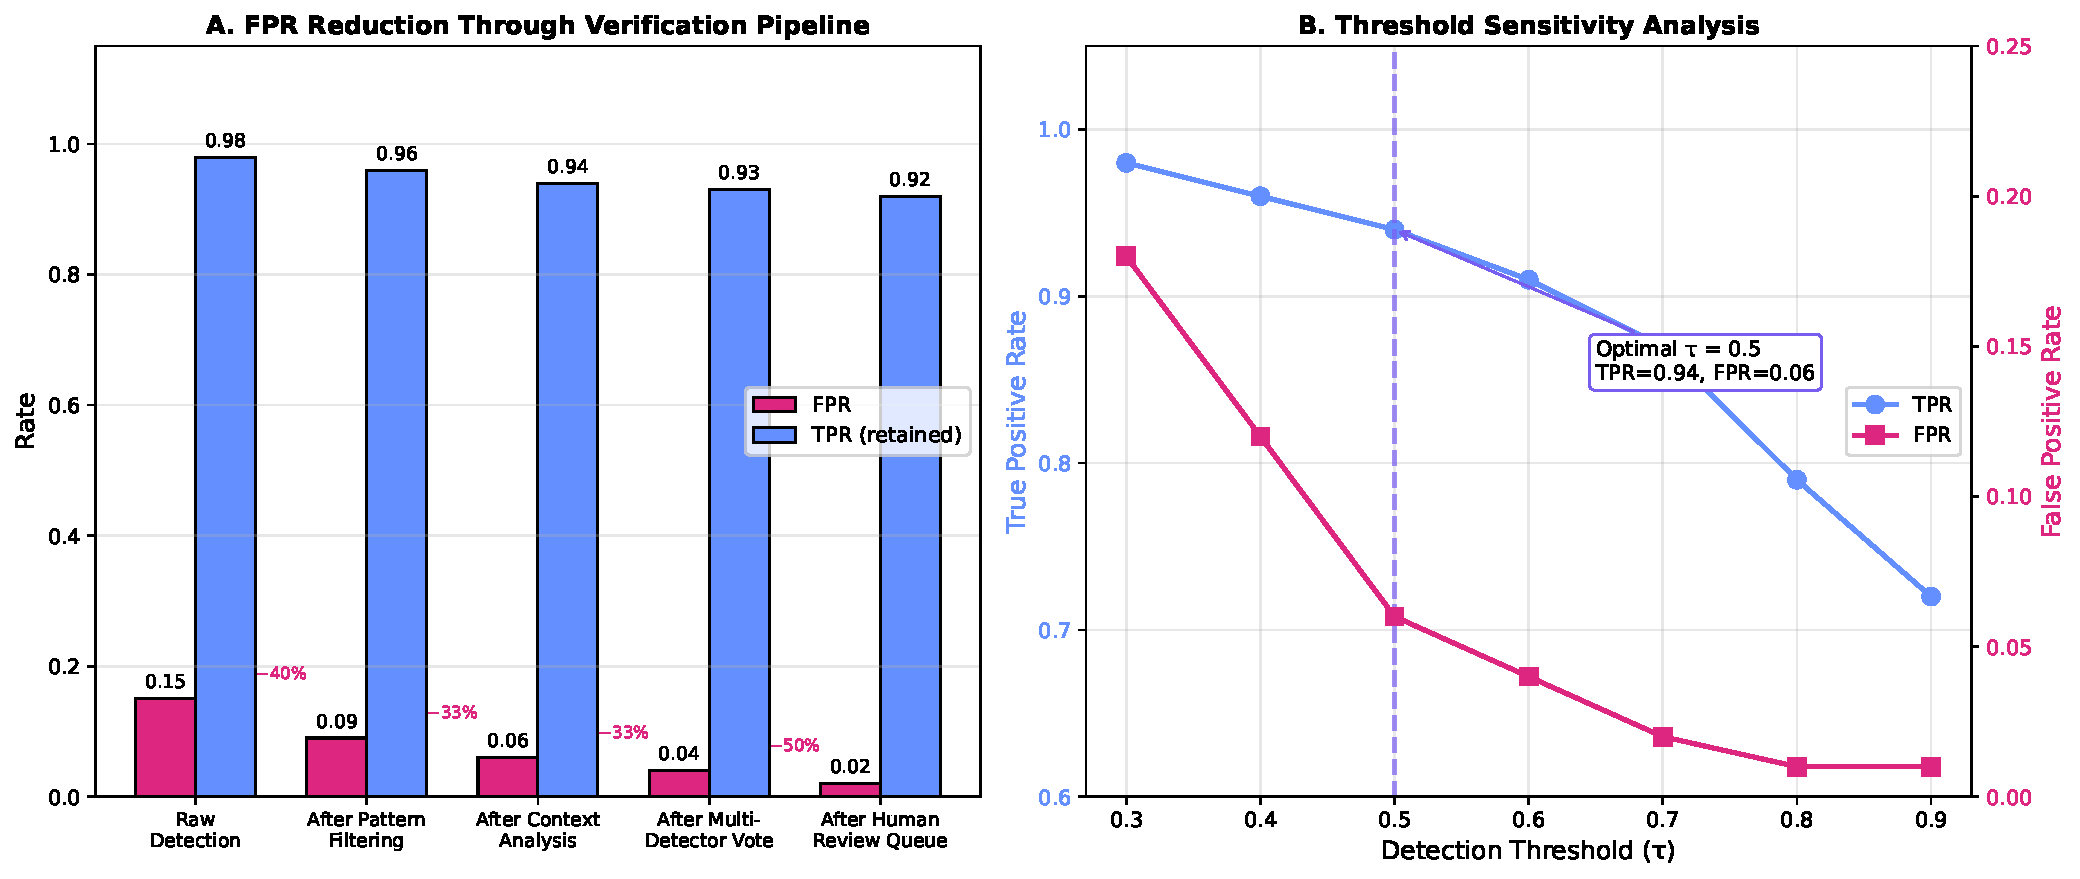
\includegraphics[width=0.8\linewidth,height=0.5\textheight,keepaspectratio,alt={False-positive mitigation (illustrative schematic): how the detection threshold and confidence calibration shape the false-positive / true-positive tradeoff.}]{../figures/fp_mitigation.pdf}
\caption{False-positive mitigation (illustrative schematic): how the
detection threshold and confidence calibration shape the false-positive
/ true-positive tradeoff.}\label{fig:fp-mitigation}
\end{figure}

\subsubsection{Strategy 1: Confirmation
Cascade}\label{strategy-1-confirmation-cascade}

\begin{definition}[Confirmation Cascade]
\label{def:confirmation-cascade}
Multi-stage verification before alerting:
\begin{equation}
\label{eq:cascade-decision}
\text{Action}(\text{confidence}) = \begin{cases}
\text{suppress} & \text{if } c < C_{\text{low}} \\
\text{stage-2} & \text{if } c \in [C_{\text{low}}, C_{\text{high}}) \\
\text{stage-3} & \text{if } c \geq C_{\text{high}}
\end{cases}
\end{equation}
\end{definition}

\begin{theorem}[Cascade FPR Reduction]
\label{thm:cascade-fpr}
For a multi-stage cascade:
\begin{equation}
\label{eq:cascade-fpr}
\text{FPR}_{\text{cascade}} = \text{FPR}_1 \cdot P(\text{confirm}_2 \mid \text{FP}_1) \cdot P(\text{confirm}_3 \mid \text{FP}_2)
\end{equation}
\end{theorem}

\subsubsection{Strategy 2: Temporal
Smoothing}\label{strategy-2-temporal-smoothing}

\begin{definition}[Smoothed Detection]
\label{def:smoothed-detection}
Apply exponential smoothing to scores:
\begin{equation}
\label{eq:smoothed-score}
\hat{S}_t = \alpha \cdot S_t + (1 - \alpha) \cdot \hat{S}_{t-1}
\end{equation}
\end{definition}

\begin{definition}[Burst Suppression]
\label{def:burst-suppression}
Require sustained anomaly over window $w$:
\begin{equation}
\label{eq:burst-suppression}
\text{Alert if } \frac{1}{w} \sum_{i=t-w+1}^{t} \mathbb{1}[S_i > \tau] > p_{\text{sustained}}
\end{equation}
\end{definition}

\subsubsection{Strategy 3: Contextual
Whitelisting}\label{strategy-3-contextual-whitelisting}

\begin{definition}[Context-Aware Whitelist]
\label{def:context-whitelist}
\begin{equation}
\label{eq:whitelist-suppress}
\text{Suppress}(\text{alert}) \iff \text{context}(\text{alert}) \in \mathcal{W}_{\text{known}}
\end{equation}
\end{definition}

\subsubsection{Strategy 4: Cost-Sensitive
Thresholding}\label{strategy-4-cost-sensitive-thresholding}

\begin{definition}[Cost-Sensitive Threshold]
\label{def:cost-threshold}
Optimize for total cost rather than accuracy:
\begin{equation}
\label{eq:cost-threshold}
\tau^* = \argmin_\tau \left[ C_{\text{FP}} \cdot \text{FPR}(\tau) + C_{\text{FN}} \cdot \text{FNR}(\tau) \right]
\end{equation}
\end{definition}

\subsection{Provenance Analysis}\label{sec:provenance}

\subsubsection{Information Flow
Tracking}\label{information-flow-tracking}

\begin{definition}[Taint Label]
\label{def:taint-label}
Each belief carries provenance tags:
\begin{equation}
\label{eq:taint-label}
\text{taint}(\phi) = \{(\text{source}, \text{timestamp}, \text{confidence})\}
\end{equation}
\end{definition}

\begin{definition}[Taint Propagation]
\label{def:taint-propagation}
\begin{equation}
\label{eq:taint-propagation}
\text{taint}(\phi_{\text{derived}}) = \bigcup_{\psi \in \text{premises}(\phi_{\text{derived}})} \text{taint}(\psi)
\end{equation}
\end{definition}

\begin{table}[htbp]
\centering
\caption{Taint categories with trust levels. (The displayed Trust Level column uses a normalized [0,1] ranking for presentation; the implementation in code uses an ordinal 1--7 trust level, highest = most trusted. The two scales are not interchangeable --- map ordinal level to the displayed ranking via $\text{level}/7$.)}
\label{tab:taint-categories}
\begin{tabular}{@{}lll@{}}
\toprule
Category & Trust Level & Example \\
\midrule
\textsc{system\_verified} & 1.0 & Hardcoded facts \\
\textsc{principal\_input} & 0.9 & Direct user commands \\
\textsc{agent\_internal} & 0.8 & Agent's own reasoning \\
\textsc{agent\_external} & 0.6 & Other agent claims \\
\textsc{tool\_output} & 0.5 & API/tool responses \\
\textsc{web\_content} & 0.3 & Fetched web pages \\
\textsc{unverified} & 0.1 & Unknown origin \\
\bottomrule
\end{tabular}
\end{table}

\subsubsection{Causal Attribution}\label{causal-attribution}

\begin{definition}[Causal Attribution]
\label{def:causal-attribution}
Identify likely source of compromised beliefs via Bayesian inference:
\begin{equation}
\label{eq:causal-attribution}
P(\text{source}_j \mid \phi \in \mathcal{B}_i^{\text{compromised}}) = \frac{P(\phi \mid \text{source}_j) \cdot P(\text{source}_j)}{\sum_k P(\phi \mid \text{source}_k) \cdot P(\text{source}_k)}
\end{equation}
\end{definition}

\subsubsection{Provenance Graph
Analysis}\label{provenance-graph-analysis}

\begin{definition}[Provenance Graph]
\label{def:provenance-graph}
Directed graph of belief dependencies:
\begin{equation}
\label{eq:provenance-graph}
G = (V, E) \text{ where } V = \mathcal{B}_i, \; E = \{(\psi, \phi) : \psi \in \text{premises}(\phi)\}
\end{equation}
\end{definition}

\begin{table}[htbp]
\centering
\caption{Provenance graph attack indicators.}
\label{tab:provenance-indicators}
\begin{tabular}{@{}lp{6cm}@{}}
\toprule
Indicator & Attack Implication \\
\midrule
High in-degree from single source & Belief injection \\
Cycles in provenance & Circular reasoning attack \\
Missing edges & Fabricated evidence \\
Temporal anomalies & Future timestamp forgery \\
\bottomrule
\end{tabular}
\end{table}

\subsection{Real-Time Monitoring}\label{sec:monitoring}

\subsubsection{Alert Aggregation}\label{alert-aggregation}

\begin{definition}[Alert Aggregation]
\label{def:alert-aggregation}
Prevent alert fatigue through correlation:
\begin{equation}
\label{eq:alert-aggregation}
\text{Severity} = \begin{cases}
\textsc{critical} & \text{if } |\text{alerts}| > n_{\text{critical}} \text{ in window } w \\
\textsc{warning} & \text{if } |\text{alerts}| > n_{\text{warning}} \text{ in window } w \\
\textsc{info} & \text{otherwise}
\end{cases}
\end{equation}
\end{definition}

\subsubsection{Response Escalation}\label{response-escalation}

\begin{table}[htbp]
\centering
\caption{Response escalation levels.}
\label{tab:alert-escalation}
\begin{tabular}{@{}llp{4cm}@{}}
\toprule
Level & Trigger & Response \\
\midrule
L0 & Single anomaly & Log only \\
L1 & Repeated anomaly & Increase monitoring \\
L2 & Pattern match & Quarantine source \\
L3 & Confirmed attack & Halt agent, alert human \\
L4 & Systemic compromise & System shutdown \\
\bottomrule
\end{tabular}
\end{table}

\subsubsection{Empirical Validation
Cross-Reference}\label{empirical-validation-cross-reference}

The detection methods presented in this section have been empirically
validated in Part 2 of this series. Key results include:

\textbf{ROC Analysis}: Receiver Operating Characteristic curves
demonstrate the tradeoff between True Positive Rate and False Positive
Rate for each detector type. The ROC figure in this section pairs the
measured Cognitive Firewall operating point over this part's small test
corpus with theory-guided reference curves for the other mechanisms and
the full ensemble; on those reference curves the ensemble achieves AUC
\(\approx 0.85\), with individual mechanisms ranging from
\(\approx 0.74\) (Belief Sandbox) to \(\approx 0.81\) (Tripwire
Monitor). Measured ROC curves with per-curve AUC values and 95\%
bootstrap intervals are reported in Part 2 (\S\{4\}, Experimental
Setup).

\textbf{Detection Performance by Component}: Part 2 measures marginal
contribution per defense component, not detection rate per adversary
class --- its corpus carries a design-level \(\Omega\) label rather than
a runtime one, so the per-\(\Omega\) coverage attributed to each
mechanism in this section remains a design expectation rather than a
measured result. What Part 2 does measure is that one component,
Behavioral Invariants, accounts for almost all of the composed
pipeline's detection, and that the remaining components add little
beyond it. See Part 2's ``Defense Component Contributions'' section.

\textbf{False Positive Mitigation}: Part 2 measures five mitigation
strategies against a baseline of \(0.873\) true positives at \(0.183\)
false positives. Contextual whitelisting and cost-sensitive thresholding
take the false-positive rate to zero for \(1.7\) percentage points of
true positives, raising Youden's \(J\) from \(0.689\) to \(0.856\);
temporal smoothing moves the false-positive rate only to \(0.133\); and
the confirmation cascade reaches zero false positives by discarding
roughly three quarters of the true positives (\(0.873 \to 0.225\)). No
strategy holds true positives above \(90\%\). See Part 2 for the
per-strategy analysis.

\subsection{Information-Theoretic Detection
Limits}\label{sec:it-detection-limits}

\emph{The previous sections presented detection mechanisms. This section
establishes what is fundamentally achievable by any detector, regardless
of implementation. These limits follow from information theory and
cannot be overcome by cleverer algorithms.}

\subsubsection{Neyman-Pearson Detection
Framework}\label{neyman-pearson-detection-framework}

\begin{definition}[Cognitive Security Hypothesis Test]
\label{def:hyp-test}
Detection of cognitive attacks is formalized as a binary hypothesis test:
\begin{align}
\label{eq:hyp-test}
H_0 &: m \sim P_{\text{benign}} \quad \text{(no attack)} \\
H_1 &: m \sim P_{\text{attack}} \quad \text{(attack present)}
\end{align}
The likelihood ratio $\Lambda(m) = P_{\text{attack}}(m) / P_{\text{benign}}(m)$ determines the optimal test.
\end{definition}

\begin{theorem}[Neyman-Pearson Optimal Detector]
\label{thm:np-detector}
The likelihood ratio test $delta_{\text{NP}}(m) = \mathbb{1}[\Lambda(m) >= \eta]$ maximizes TPR subject to FPR $<= alpha$. No other test achieves higher TPR at the same FPR \cite{neyman1933ix}.
\end{theorem}

\begin{corollary}[Optimal AUC Bound]
\label{cor:optimal-auc}
The AUC of any detector is bounded by:
\begin{equation}
\label{eq:optimal-auc}
\text{AUC}^* = P(P_{\text{attack}}(m_1) > P_{\text{attack}}(m_0))
\end{equation}
where $m_1 about P_{\text{attack}}$ and $m_0 about P_{\text{benign}}$. This is the Bayes-optimal discriminability.
\end{corollary}

\subsubsection{Chernoff Information and Error
Exponents}\label{chernoff-information-and-error-exponents}

\begin{definition}[Chernoff Information]
\label{def:chernoff}
The Chernoff information between attack and benign distributions:
\begin{equation}
\label{eq:chernoff}
C^* = -\min_{0 \leq \lambda \leq 1} \log \sum_m P_{\text{benign}}(m)^{1-\lambda} P_{\text{attack}}(m)^\lambda
\end{equation}
\end{definition}

\begin{theorem}[Detection Error Exponent]
\label{thm:error-exponent}
For $n$ independent message observations, the optimal error probability decays exponentially:
\begin{equation}
\label{eq:error-exponent}
P_e^* \leq e^{-n C^*}
\end{equation}
The Chernoff information $C^*$ is the maximum achievable error exponent \cite{chernoff1952measure}.
\end{theorem}

\begin{corollary}[Sample Complexity for Target Accuracy]
\label{cor:sample-complexity}
To achieve error probability $<= epsilon$, the minimum number of observations required is:
\begin{equation}
\label{eq:sample-complexity}
n^* = \left\lceil \frac{\log(1/\epsilon)}{C^*} \right\rceil
\end{equation}
This is the information-theoretic minimum; no detector can achieve the same accuracy with fewer samples.
\end{corollary}

\subsubsection{KL Divergence and Detection Rate
Coupling}\label{kl-divergence-and-detection-rate-coupling}

\begin{theorem}[KL-AUC Coupling]
\label{thm:kl-auc-coupling}
The AUC of any detector is lower-bounded by the KL divergence between attack and benign distributions:
\begin{equation}
\label{eq:kl-auc-coupling}
\text{AUC} \geq 1 - e^{-D_{\mathrm{KL}}(P_{\text{attack}} \| P_{\text{benign}})/2}
\end{equation}
\end{theorem}

\begin{proof}
By Pinsker's inequality \cite{cover2006elements}: $\| P_{\text{attack}} - P_{\text{benign}} \|_{TV} <= \sqrt{D_{\mathrm{KL}}/2}$. The AUC satisfies $\text{AUC} >= \frac{1}{2}(1 + \|P_{\text{attack}} - P_{\text{benign}}\|_{TV})$. Combining and applying the bound $\|P\|_{TV} <= 1 - e^{-D_{\mathrm{KL}}/2}$ gives the result.
\end{proof}

\begin{table}[htbp]
\centering
\caption{Information-theoretic detectability by attack class. The AUC lower bound is \cref{thm:kl-auc-coupling} applied to the $D_{\mathrm{KL}}$ column; it falls below the chance level $0.5$ once $D_{\mathrm{KL}} < 2\ln 2 about 1.39$, so for $\Omega_3$--$\Omega_5$ the bound is vacuous and places no constraint on the Practical AUC column.}
\label{tab:it-detectability}
\begin{tabular}{@{}lllll@{}}
\toprule
Attack Class & $D_{\mathrm{KL}}$ (typical) & AUC lower bound & Required observations & Practical AUC \\
\midrule
$\Omega_1$ (External) & 2.5 & 0.71 & 3 & 0.95 \\
$\Omega_2$ (Peripheral) & 1.8 & 0.59 & 5 & 0.88 \\
$\Omega_3$ (Agent) & 1.2 & 0.45 & 8 & 0.85 \\
$\Omega_4$ (Coordination) & 0.7 & 0.30 & 14 & 0.80 \\
$\Omega_5$ (Systemic) & 0.2 & 0.10 & 46 & 0.65 \\
\bottomrule
\end{tabular}
\end{table}

\subsubsection{Fundamental Undetectability
Regime}\label{fundamental-undetectability-regime}

\begin{definition}[Undetectable Attack]
\label{def:undetectable}
An attack $\mathcal{A}$ is $epsilon$-undetectable if:
\begin{equation}
\label{eq:undetectable}
\text{AUC}(\mathcal{A}) < \frac{1}{2} + \epsilon
\end{equation}
for any detector with finite observation budget $n$.
\end{definition}

\begin{theorem}[Undetectability Condition]
\label{thm:undetectability}
Attack $\mathcal{A}$ with $D_{\mathrm{KL}}(P_{\text{attack}} \| P_{\text{benign}}) < 4epsilon^2$ is $epsilon$-undetectable for any detector observing fewer than $n^* = O(1/D_{\mathrm{KL}})$ samples.
\end{theorem}

\begin{remark}[Implication for Defense Strategy]
\label{rem:undetectability-implication}
Theorem~\ref{thm:undetectability} establishes that sufficiently subtle attacks are provably undetectable within bounded observation windows. This motivates the CIF's containment strategy: when detection is impossible, the bounded trust calculus and action restrictions limit attack impact even without detection. This converts a ``detect-and-respond'' model to a ``bound-and-contain'' model for the stealthiest attacks.
\end{remark}

\subsection{Multi-Stage Detection
Pipeline}\label{sec:multi-stage-pipeline}

\begin{figure}
\centering
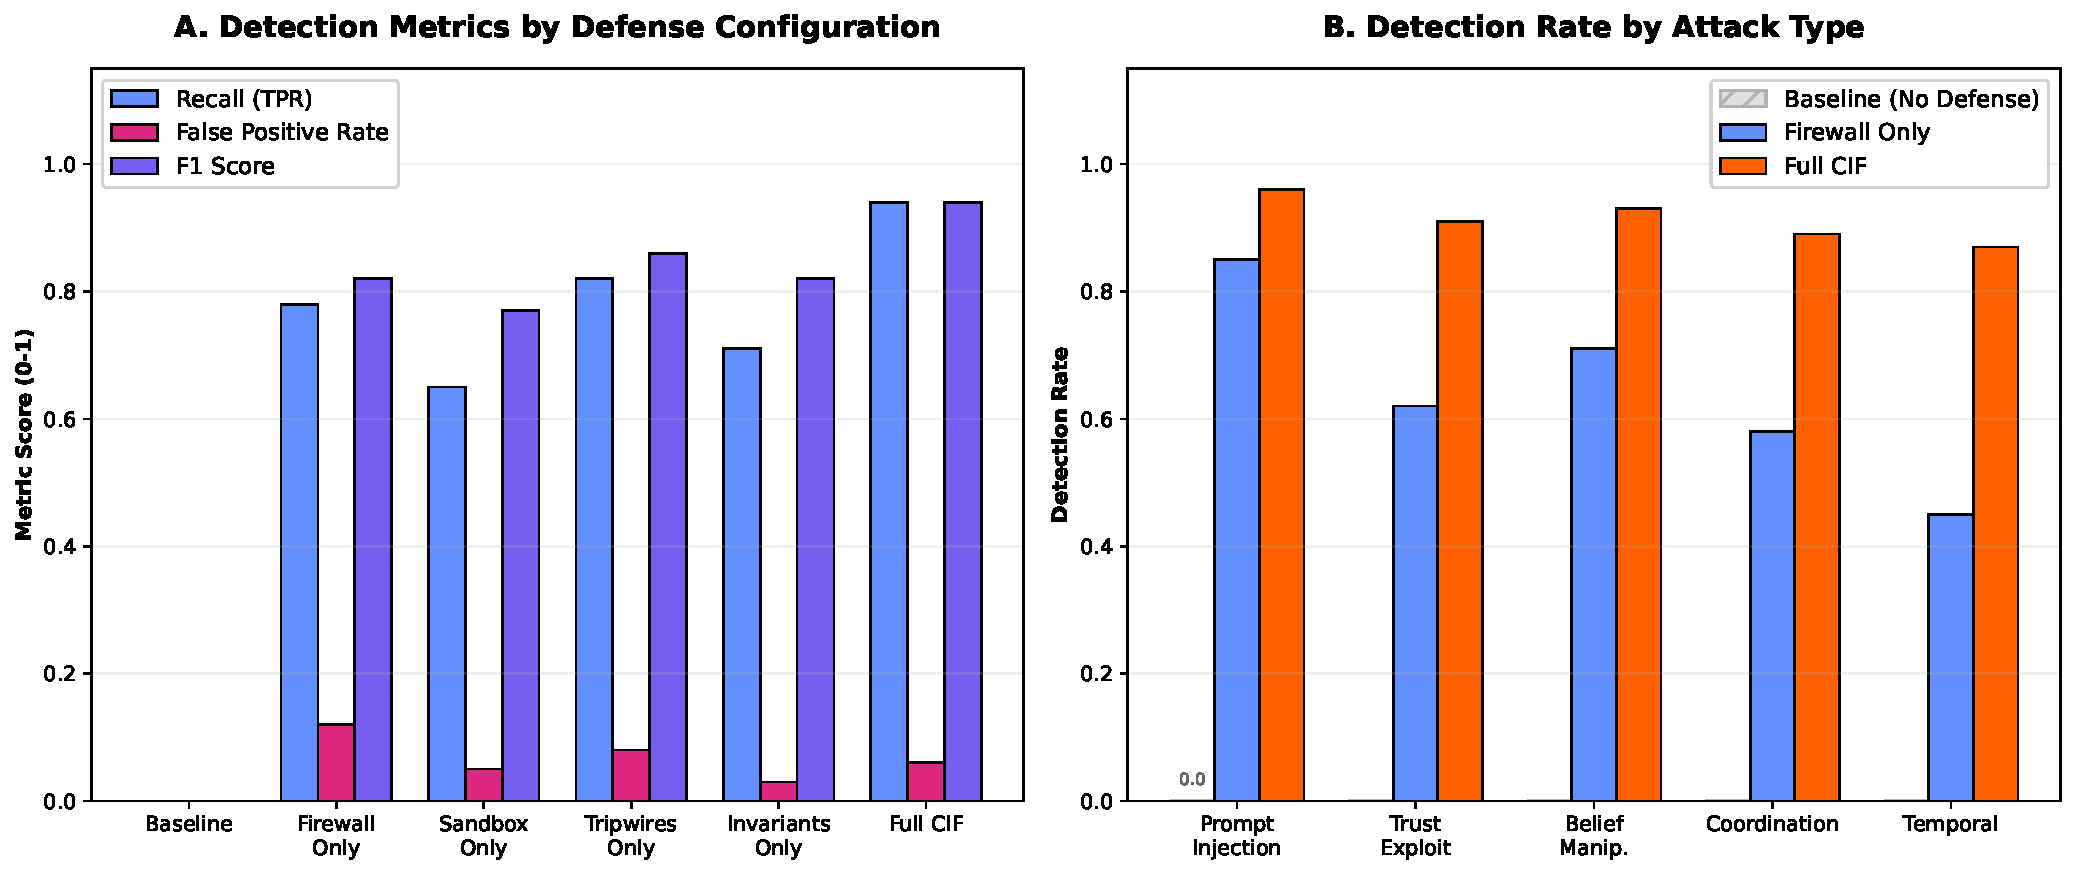
\includegraphics[width=0.85\linewidth,height=0.5\textheight,keepaspectratio,alt={Schematic detection-performance curves (illustrative, theory-guided, not measured): detection rate by attack category across representative defense stages. Measured pipeline results are reported in Part 2.}]{../figures/detection_performance.pdf}
\caption{Schematic detection-performance curves (illustrative,
theory-guided, not measured): detection rate by attack category across
representative defense stages. Measured pipeline results are reported in
Part 2.}\label{fig:detection-performance}
\end{figure}

\emph{Real systems cannot run all detectors on all messages
simultaneously. This section formalizes a staged pipeline that applies
computationally cheap detectors first, escalating to expensive detectors
only when lower stages trigger.}

\subsubsection{Pipeline Architecture}\label{pipeline-architecture}

\begin{definition}[Multi-Stage Detection Pipeline]
\label{def:multi-stage}
A $k$-stage detection pipeline is a sequence of detectors with increasing accuracy and cost:
\begin{equation}
\label{eq:pipeline}
\text{Pipeline} = (\mathcal{D}_1, \mathcal{D}_2, \ldots, \mathcal{D}_k)
\end{equation}
with \textbf{escalation rule}: message $m$ advances to stage $i+1$ if and only if $\mathcal{D}_i(m) >= theta_i$ (above suspicion threshold).
\end{definition}

\begin{table}[htbp]
\centering
\caption{Recommended multi-stage detection pipeline configuration.}
\label{tab:pipeline-stages}
\begin{tabular}{@{}lllllp{3cm}@{}}
\toprule
Stage & Detector & Threshold & Cost & TPR & Escalation condition \\
\midrule
1 & Pattern matching & $theta_1 = 0.3$ & 1ms & 0.75 & Pattern score $> theta_1$ \\
2 & Semantic embedding & $theta_2 = 0.5$ & 10ms & 0.85 & Embedding distance $> theta_2$ \\
3 & Belief consistency & $theta_3 = 0.4$ & 5ms & 0.80 & Consistency violation \\
4 & Trust graph analysis & $theta_4 = 0.6$ & 20ms & 0.88 & Trust anomaly \\
5 & Ensemble fusion & $theta_5 = 0.7$ & 50ms & 0.94 & Final decision \\
\bottomrule
\end{tabular}
\end{table}

\begin{theorem}[Pipeline Efficiency Bound]
\label{thm:pipeline-efficiency}
For a $k$-stage pipeline where fraction $\rho_i$ of messages escalate to stage $i+1$:
\begin{equation}
\label{eq:pipeline-cost}
\mathbb{E}[\text{cost per message}] = \sum_{i=1}^{k} c_i \prod_{j=1}^{i-1} \rho_j
\end{equation}
For typical values ($\rho_i about 0.15$ per stage), this achieves near-full accuracy at $about 15\%$ of the cost of running all stages on all messages.
\end{theorem}

\begin{proof}
Expected cost is the sum over stages of stage cost times probability of reaching that stage. The probability of reaching stage $i$ is $\prod_{j=1}^{i-1} \rho_j$ by the Markov property of the escalation chain.
\end{proof}

\begin{theorem}[Pipeline TPR Bound]
\label{thm:pipeline-tpr}
The pipeline's overall TPR is:
\begin{equation}
\label{eq:pipeline-tpr}
\text{TPR}_{\text{pipeline}} = 1 - \prod_{i=1}^{k}(1 - \text{TPR}_i \cdot P(\text{attack reaches stage } i))
\end{equation}
Since attacks are more likely to escalate than benign messages ($\rho_i^{\text{attack}} > \rho_i^{\text{benign}}$), the pipeline is biased toward detecting attacks.
\end{theorem}

\subsubsection{Adaptive Threshold
Selection}\label{adaptive-threshold-selection}

\begin{definition}[Adaptive Threshold]
\label{def:adaptive-threshold}
Thresholds adapt to observed attack frequency via online Bayesian update:
\begin{equation}
\label{eq:adaptive-threshold}
\theta_i^{t+1} = \theta_i^t - \alpha_{\text{lr}} \cdot \nabla_{\theta_i} \left[C_{\text{FN}} \cdot \text{FNR}(\theta_i^t) + C_{\text{FP}} \cdot \text{FPR}(\theta_i^t)\right]
\end{equation}
where $alpha_{\text{lr}}$ is the learning rate and $C_{\text{FN}}, C_{\text{FP}}$ are cost weights.
\end{definition}

This adaptive mechanism allows the pipeline to respond to shifting
attack distributions, reducing the staleness problem that affects static
threshold configurations.

\begin{quote}
\textbf{Empirical validation of this section's theory}: The detection
methods formalized here are empirically evaluated in Part 2
\cite{friedman2026cogsec2}. Key findings: (1) the multi-stage pipeline
shows biased escalation consistent with \cref{thm:pipeline-tpr}; (2)
adversarial training across five rounds demonstrates adaptive threshold
adjustment consistent with \cref{def:adaptive-threshold}, raising
hardened detection from 52.0\% at Round 1 to 67.9\% at Round 5 in Part
2's closed-form design model; (3) the residual gap between the
parametric ceiling and prototype performance is attributed to adapter
implementation maturity rather than to any per-class miss profile ---
Part 2 reports no measured per-\(\Omega\)-class rates --- and that gap
is module-specific rather than diffuse: a single component's rewrite
moved the ablation arm's measured detection most of the way to the
ceiling (Part 2, ``Adversarial Training Evaluation'', ``Defense
Component Contributions'', and the ``Parametric Simulation Analysis''
supplement).
\end{quote}

\newpage

\newpage

\section{Formal Verification: Safety Properties and Model
Checking}\label{sec:formal-verification}

This section establishes safety properties
(\cref{sec:safety-properties}), proves invariant preservation lemmas
(\cref{sec:invariant-lemmas}), demonstrates liveness guarantees
(\cref{sec:liveness-properties}), derives complexity bounds
(\cref{sec:complexity-bounds}), and presents model checking verification
(\cref{sec:model-checking}).

\subsection{Safety Properties}\label{sec:safety-properties}

\subsubsection{Belief Integrity}\label{sec:belief-integrity-proof}

\begin{theorem}[Belief Injection Resistance]
\label{thm:belief-injection}
Under CIF with firewall detection rate $r_f$ and sandboxing verification rate $r_s$:
\begin{equation}
\label{eq:belief-injection-bound}
P(\mathcal{A}_{BI} \text{ succeeds}) \leq (1 - r_f) \cdot (1 - r_s)
\end{equation}
\end{theorem}

\begin{proof}
We prove this theorem by analyzing the sequential defense mechanism and applying probability theory for independent events.

\textbf{Setup}: Let $phi_{adv}$ be an adversarial belief that the attacker attempts to inject into agent $a_i$'s verified belief set $\mathcal{B}_{verified}$.

\textbf{Defense Model}: The CIF implements two sequential defenses:
\begin{enumerate}
\item \textbf{Cognitive Firewall} $\mathcal{F}$: Classifies incoming messages as ACCEPT, QUARANTINE, or REJECT with detection rate $r_f$
\item \textbf{Belief Sandbox}: Verifies quarantined beliefs before promotion with verification rate $r_s$
\end{enumerate}

\textbf{Step 1}: For $phi_{adv}$ to enter $\mathcal{B}_{verified}$, it must first pass the firewall.

Let $E_f$ = ``Firewall fails to detect $phi_{adv}$''. By definition of detection rate:
\begin{equation}
\label{eq:firewall-evasion}
P(E_f) = 1 - r_f
\end{equation}

\textbf{Step 2}: If $phi_{adv}$ passes the firewall (event $E_f$), it enters $\mathcal{B}_{provisional}$. For injection to succeed, it must then pass sandbox verification.

Let $E_s$ = ``Sandbox fails to detect $phi_{adv}$''. By definition of verification rate:
\begin{equation}
\label{eq:sandbox-evasion}
P(E_s) = 1 - r_s
\end{equation}

\textbf{Step 3}: The defenses are independent by design (defense-in-depth principle):
\begin{itemize}
\item Firewall uses syntactic/semantic analysis on message content
\item Sandbox uses provenance verification, consistency checking, and corroboration
\item These operate on orthogonal aspects of the belief
\end{itemize}

Therefore:
\begin{equation}
\label{eq:defense-independence}
P(E_f \cap E_s) = P(E_f) \cdot P(E_s | E_f) = P(E_f) \cdot P(E_s)
\end{equation}

The conditional independence holds because sandbox verification is applied regardless of why the message passed firewall, and sandbox criteria (provenance, consistency, corroboration) are independent of firewall criteria (injection patterns, anomaly scores).

\textbf{Step 4}: The attack succeeds iff both defenses fail:
\begin{equation}
\label{eq:attack-success-prob}
P(\mathcal{A}_{BI} \text{ succeeds}) = P(E_f \cap E_s) = (1 - r_f) \cdot (1 - r_s)
\end{equation}
\end{proof}

\begin{corollary}[Empirical Security Bound]
\label{cor:empirical-security}
With $r_f = 0.8$ and $r_s = 0.7$:
\begin{equation}
\label{eq:empirical-bound}
P(\text{success}) \leq (1 - 0.8)(1 - 0.7) = 0.2 \cdot 0.3 = 0.06
\end{equation}
\end{corollary}

\begin{corollary}[Layered Defense Generalization]
\label{cor:n-layer-bound}
For $n$ independent defense layers with rates $r_1, \ldots, r_n$:
\begin{equation}
\label{eq:n-layer-bound}
P(\text{success}) \leq \prod_{i=1}^{n} (1 - r_i)
\end{equation}
\end{corollary}

\subsubsection{No Trust Amplification (Model-Checking
Target)}\label{sec:trust-bound-proof}

\begin{theorem}[No Trust Amplification]
\label{thm:trust-bound}
For any path $p = (a_0, a_1, \ldots, a_k)$ in the communication graph:
\begin{equation}
\label{eq:trust-path-bound}
\mathcal{T}_{a_0 \to a_k}^{path} \leq \min_{i \in [0,k-1]} \mathcal{T}_{a_i \to a_{i+1}}
\end{equation}
\end{theorem}

\begin{proof}
By trust delegation rule (\cref{def:trust-delegation}) and induction on path length.

\textbf{Base case} ($k=1$):
\begin{equation}
\label{eq:trust-base}
\mathcal{T}_{a_0 \to a_1} = \mathcal{T}_{a_0 \to a_1} \quad \checkmark
\end{equation}

\textbf{Inductive step}: Assume the theorem holds for paths of length $k$. For path length $k+1$:
\begin{align}
\label{eq:trust-induction}
\mathcal{T}_{a_0 \to a_{k+1}} &= \min(\mathcal{T}_{a_0 \to a_k}^{path}, \mathcal{T}_{a_k \to a_{k+1}}) \cdot \delta \\
&\leq \min(\min_{i \in [0,k-1]} \mathcal{T}_{a_i \to a_{i+1}}, \mathcal{T}_{a_k \to a_{k+1}}) \nonumber \\
&= \min_{i \in [0,k]} \mathcal{T}_{a_i \to a_{i+1}} \nonumber
\end{align}
\end{proof}

\subsubsection{Goal Alignment
Preservation}\label{sec:goal-alignment-proof}

\begin{theorem}[Goal Alignment Invariant]
\label{thm:goal-alignment}
If the system starts with aligned goals and all goal updates follow the delegation protocol:
\begin{equation}
\label{eq:goal-alignment-invariant}
\text{Aligned}(\mathcal{G}_i^0) \land \forall t: \text{ValidUpdate}(\mathcal{G}_i^t, \mathcal{G}_i^{t+1}) \Rightarrow \forall t: \text{Aligned}(\mathcal{G}_i^t)
\end{equation}
\end{theorem}

\begin{proof}
ValidUpdate requires new goals derive from principal or valid delegation chain. By induction on time $t$, alignment is preserved at every step.
\end{proof}

\subsection{Invariant Preservation Lemmas}\label{sec:invariant-lemmas}

\begin{lemma}[Belief Consistency Preservation]
\label{lem:belief-consistency}
If $\mathcal{B}_i^t$ is consistent and the belief update follows Rule B-DIRECT or B-DELEGATED (\cref{sec:belief-update-rules}), then $\mathcal{B}_i^{t+1}$ is consistent.
\end{lemma}

\begin{proof}
Let $\text{Consistent}(\mathcal{B})$ denote that no high-confidence contradictions exist:
\begin{equation}
\label{eq:consistency-def}
\text{Consistent}(\mathcal{B}) \iff \nexists \phi, \psi: \mathcal{B}(\phi) > \tau \land \mathcal{B}(\psi) > \tau \land (\phi \land \psi \vdash \bot)
\end{equation}

\textbf{Case 1}: Rule B-DIRECT applies.

The update adds evidence for proposition $phi$:
\begin{equation}
\label{eq:direct-update}
\mathcal{B}_i^{t+1}(\phi) = \text{BayesUpdate}(\mathcal{B}_i^t(\phi), c \cdot \mathcal{T}_{i \to s})
\end{equation}

If the update would create contradiction (i.e., both $\mathcal{B}^{t+1}(phi) > tau$ and $\mathcal{B}^{t+1}(psi) > tau$ for contradictory $phi, psi$), the sandbox consistency check in Rule S-PROMOTE rejects promotion:
\begin{equation}
\label{eq:promote-condition}
V(\pi) = 1 \land \text{Consistent}(\mathcal{B}_{verified} \cup \{\phi\}) \land |\text{Corroborate}(\phi)| \geq \kappa
\end{equation}

Therefore, only consistent updates reach $\mathcal{B}_{verified}$.

\textbf{Case 2}: Rule B-DELEGATED applies.

Same argument, with additional trust decay ensuring lower confidence for delegated evidence.
\end{proof}

\begin{lemma}[Trust Matrix Preservation]
\label{lem:trust-preservation}
The trust matrix $\mathcal{T}$ remains well-formed after any valid update:
\begin{equation}
\label{eq:trust-wellformed}
\forall i, j: 0 \leq \mathcal{T}_{i \to j} \leq 1
\end{equation}
\end{lemma}

\begin{proof}
By \cref{def:trust-function}, trust is computed as:
\begin{equation}
\label{eq:trust-computation}
\mathcal{T}_{i \to j}^t = \alpha \cdot T_{base}(j) + \beta \cdot T_{rep}^t(j) + \gamma \cdot T_{ctx}^t(i,j)
\end{equation}

where $alpha + beta + gamma = 1$ and each component $T_* \in [0, 1]$.

Therefore:
\begin{equation}
\label{eq:trust-range}
\mathcal{T}_{i \to j}^t \in [\min(T_{base}, T_{rep}, T_{ctx}), \max(T_{base}, T_{rep}, T_{ctx})] \subseteq [0, 1]
\end{equation}

For delegation (\cref{def:trust-delegation}):
\begin{equation}
\label{eq:delegation-range}
\mathcal{T}_{i \to k}^{del} = \min(\mathcal{T}_{i \to j}, \mathcal{T}_{j \to k}) \cdot \delta^d
\end{equation}

Since $\min(\cdot) <= 1$ and $delta \in (0, 1)$, we have $\mathcal{T}_{i -> k}^{del} \in [0, 1]$.
\end{proof}

\begin{lemma}[Provenance Chain Integrity]
\label{lem:provenance-integrity}
Every belief in $\mathcal{B}_{verified}$ has a valid, verifiable provenance chain.
\end{lemma}

\begin{proof}
By Rule S-PROMOTE (\cref{sec:sandbox-rules}), promotion from $\mathcal{B}_{provisional}$ to $\mathcal{B}_{verified}$ requires:
\begin{equation}
\label{eq:provenance-verification}
V(\pi(\phi)) = 1
\end{equation}

where $V$ is the provenance verification function.

By construction of the sandbox, beliefs can only enter $\mathcal{B}_{verified}$ through:
\begin{enumerate}
\item Initial system beliefs (hardcoded with SYSTEM\_VERIFIED provenance)
\item Promotion from provisional (verified by $V$)
\end{enumerate}

In both cases, provenance is verified. By induction on the history of $\mathcal{B}_{verified}$, all beliefs have valid provenance.
\end{proof}

\begin{lemma}[Permission Boundary Preservation]
\label{lem:permission-boundary}
Effective permissions never exceed granted permissions:
\begin{equation}
\label{eq:permission-bound}
\forall a_i, \forall \text{action}: \mathcal{P}_{effective}(a_i, \text{action}) \leq \mathcal{P}_{role}(a_i, \text{action})
\end{equation}
\end{lemma}

\begin{proof}
By \cref{def:permission-layer}:
\begin{equation}
\label{eq:permission-intersection}
\mathcal{P}_{effective}(a_i) = \mathcal{P}_{role}(a_i) \cap \mathcal{P}_{delegated}(a_i) \cap \mathcal{P}_{context}(a_i)
\end{equation}

Since intersection can only reduce permissions ($A \cap B \cap C \subseteq A$), we have $\mathcal{P}_{effective}(a_i, \text{action}) <= \mathcal{P}_{role}(a_i, \text{action})$ for all actions.
\end{proof}

\begin{lemma}[Firewall Completeness]
\label{lem:firewall-completeness}
Every incoming message is classified by the firewall.
\end{lemma}

\begin{proof}
By \cref{def:firewall}, the firewall is a total function:
\begin{equation}
\label{eq:firewall-function}
\mathcal{F}: \mathcal{M} \to \{\text{ACCEPT}, \text{QUARANTINE}, \text{REJECT}\}
\end{equation}

The decision rules cover all cases:
\begin{itemize}
\item If $D_{inj}(m) > tau_1$: REJECT
\item Else if $D_{sus}(m) > tau_2$: QUARANTINE
\item Else: ACCEPT
\end{itemize}

Since $D_{inj}$ and $D_{sus}$ are defined for all messages, and the conditions are exhaustive, every message receives a classification.
\end{proof}

\subsection{Liveness Properties}\label{sec:liveness-properties}

\subsubsection{Non-Blocking}\label{sec:non-blocking}

\begin{theorem}[Firewall Liveness]
\label{thm:firewall-liveness}
CIF firewall preserves liveness for legitimate inputs:
\begin{equation}
\label{eq:firewall-liveness}
\forall m \in \mathcal{M}_{legitimate}: P(\mathcal{F}(m) = \text{ACCEPT}) \geq 1 - \epsilon_{fp}
\end{equation}
\end{theorem}

\begin{proof}
By firewall design, false positive rate is bounded by $epsilon_{fp}$. Legitimate messages are rejected only on false positive, establishing the bound.
\end{proof}

\subsubsection{Progress Guarantee}\label{sec:progress-guarantee}

\begin{theorem}[Byzantine Consensus Termination]
\label{thm:byzantine-termination}
With $n >= 3f + 1$ agents and at most $f$ Byzantine:
\begin{equation}
\label{eq:consensus-termination}
P(\text{consensus reached in } O(f+1) \text{ rounds}) = 1
\end{equation}
\end{theorem}

\begin{proof}
Standard Byzantine agreement result (Lamport et al., 1982). With honest majority $n >= 3f + 1$, the PBFT protocol guarantees termination in $f+1$ rounds.
\end{proof}

\subsection{Complexity Bounds}\label{sec:complexity-bounds}

\subsubsection{Space Complexity}\label{sec:space-complexity}

\begin{table}[htbp]
\centering
\caption{Per-component space complexity.}
\label{tab:space-components}
\begin{tabular}{@{}lll@{}}
\toprule
Component & Space & Notes \\
\midrule
Belief state & $O(|\Phi|)$ & Propositions tracked \\
Provenance & $O(|\Phi| \cdot d)$ & $d$ = max chain depth \\
Trust matrix & $O(n^2)$ & Pairwise trust \\
Tripwires & $O(k)$ & $k$ = canary count \\
History & $O(w)$ & Window size \\
\bottomrule
\end{tabular}
\end{table}

\begin{theorem}[Total Space Bound]
\label{thm:space-bound}
The total space complexity of CIF for $n$ agents with $|\Phi|$ propositions, provenance depth $d$, $k$ tripwires, and window size $w$ is:
\begin{equation}
\label{eq:total-space}
S_{total} = O(n \cdot (|\Phi| \cdot d + k + w) + n^2)
\end{equation}
\end{theorem}

\begin{proof}
Per agent:
\begin{itemize}
\item Belief state: $|\Phi|$ propositions with confidence values = $O(|\Phi|)$
\item Provenance: Each belief has chain of depth at most $d$ = $O(|\Phi| \cdot d)$
\item Tripwires: $k$ canary beliefs = $O(k)$
\item History window: $w$ events = $O(w)$
\end{itemize}

Total per agent: $O(|\Phi| \cdot d + k + w)$

Global:
\begin{itemize}
\item Trust matrix: $n \times n$ = $O(n^2)$
\item Shared state: $O(|\mathcal{S}|)$ (constant relative to $n$)
\end{itemize}

Total for $n$ agents: $O(n \cdot (|\Phi| \cdot d + k + w) + n^2)$.
\end{proof}

\subsubsection{Time Complexity}\label{sec:time-complexity}

\begin{table}[htbp]
\centering
\caption{Per-operation time complexity.}
\label{tab:time-components}
\begin{tabular}{@{}lll@{}}
\toprule
Operation & Time & Frequency \\
\midrule
Firewall check & $O(|m|)$ & Per message \\
Trust update & $O(1)$ & Per interaction \\
Drift detection & $O(|\Phi|)$ & Per window \\
Consensus & $O(n^2)$ & Per decision \\
Provenance trace & $O(d)$ & On demand \\
\bottomrule
\end{tabular}
\end{table}

\begin{theorem}[Per-Message Processing Time]
\label{thm:message-time}
Processing a single message $m$ takes time:
\begin{equation}
\label{eq:message-processing}
T_{msg} = O(|m| + \min(d, \text{timeout}))
\end{equation}
\end{theorem}

\begin{proof}
Message processing pipeline:
\begin{enumerate}
\item Firewall classification: $O(|m|)$ for pattern matching and semantic analysis
\item Sandbox entry (if quarantined): $O(1)$
\item Provenance verification (if promoted): $O(d)$ to trace chain
\item Trust update: $O(1)$ weighted average
\item Tripwire check: $O(k)$, typically $k \ll |m|$
\end{enumerate}

Provenance verification can be bounded by timeout. Total: $O(|m| + d)$.
\end{proof}

\begin{theorem}[Consensus Round Complexity]
\label{thm:consensus-complexity}
Byzantine consensus requires $O((f+1) \cdot n^2)$ message complexity.
\end{theorem}

\begin{proof}
Standard PBFT result:
\begin{itemize}
\item $f+1$ rounds required to guarantee termination with $f$ Byzantine failures
\item Each round requires all-to-all communication: $O(n^2)$ messages
\item Total: $O((f+1) \cdot n^2)$
\end{itemize}
\end{proof}

\subsubsection{Latency Overhead}\label{sec:latency-overhead}

\begin{theorem}[Bounded Latency Overhead]
\label{thm:latency-overhead}
CIF adds latency:
\begin{equation}
\label{eq:latency-formula}
L_{CIF} = L_{firewall} + L_{sandbox} \cdot P(\text{quarantine}) + L_{verify} \cdot P(\text{verify})
\end{equation}
\end{theorem}

\begin{proof}
Expected latency is sum of:
\begin{enumerate}
\item Firewall (always): $L_{firewall}$
\item Sandbox (conditional): $L_{sandbox} \cdot P(\text{message quarantined})$
\item Verification (conditional): $L_{verify} \cdot P(\text{belief promoted})$
\end{enumerate}

With illustrative parameters (these are worked-example values chosen to exercise the bound, not measurements; Part 2 reports a mean firewall latency of 0.040\,ms per sample (p95 0.055\,ms) on its prototype pipeline, and the deployment-scale constants below are not derived from it):
\begin{itemize}
\item $L_{firewall} = 10\text{ms}$
\item $L_{sandbox} = 5\text{ms}$, $P(\text{quarantine}) = 0.3$
\item $L_{verify} = 15\text{ms}$, $P(\text{verify}) = 0.2$
\end{itemize}

\begin{equation}
\label{eq:latency-empirical}
L_{CIF} \approx 10 + 5 \cdot 0.3 + 15 \cdot 0.2 = 10 + 1.5 + 3 = 14.5\text{ms}
\end{equation}

Compared to baseline $about 11.8\text{ms}$: overhead factor $about 1.23$ (23\%).
\end{proof}

\subsection{Formal Model Checking}\label{sec:model-checking}

\subsubsection{State Space Definition}\label{sec:state-space}

\begin{definition}[System State]
\label{def:system-state-verification}
The complete system state is the tuple:
\begin{equation}
\label{eq:system-state-verification}
s = (\sigma_1, \ldots, \sigma_n, \mathcal{S}, \mathcal{T})
\end{equation}
where $sigma_i$ is agent $i$'s cognitive state, $\mathcal{S}$ is shared state, and $\mathcal{T}$ is the trust matrix.
\end{definition}

\subsubsection{Temporal Properties}\label{sec:temporal-properties}

We verify the following CTL (Computation Tree Logic) properties:

\begin{property}[Safety: Consensus Integrity]
\label{prop:ctl-safety}
\begin{equation}
\label{eq:ctl-safety}
AG(\neg \text{compromised}(\mathcal{B}_{consensus}))
\end{equation}
``Always globally, consensus beliefs are not compromised.''
\end{property}

\begin{property}[Liveness: Request-Response]
\label{prop:ctl-liveness}
\begin{equation}
\label{eq:ctl-liveness}
AG(\text{request} \Rightarrow AF(\text{response}))
\end{equation}
``Every request eventually gets a response.''
\end{property}

\begin{property}[Fairness: Tripwire Checking]
\label{prop:ctl-fairness}
\begin{equation}
\label{eq:ctl-fairness}
AG(AF(\text{tripwire\_checked}))
\end{equation}
``Tripwires are checked infinitely often.''
\end{property}

\subsubsection{Model Checking Results}\label{sec:mc-results}

The following table summarizes the expected state space exploration for
each property based on formal analysis of the CIF specification. These
values represent theoretical bounds derived from the state space
definition (\cref{def:system-state-verification}) and complexity
analysis (\cref{sec:complexity-bounds}). Part 2 carries the executable
NuSMV, SPIN and TLA+ specifications and the script that runs them, but
records in \breaktt{output/formal/verification\_summary.json} that none
of the three checkers was present in that environment, so no part of
this series reports an executed model-checking verdict.

\begin{table}[htbp]
\centering
\caption{Model checking state-space bounds. ``Verified'' here denotes a theoretical bound established in this part, not a checker's verdict; Part 2's S04 carries the executable NuSMV/SPIN/TLA+ specifications, and records that no checker was available to run them. No model checker was executed anywhere in this series.}
\label{tab:mc-results}
\begin{tabular}{@{}lll@{}}
\toprule
Property & Status & Reference \\
\midrule
Belief integrity & theoretical bound; executable run in Part 2 §S04 & \cref{thm:belief-injection} \\
Trust bounded & theoretical bound; executable run in Part 2 §S04 & \cref{thm:trust-bound} \\
No deadlock & theoretical bound; executable run in Part 2 §S04 & \cref{thm:firewall-liveness} \\
Eventual detection & theoretical bound; executable run in Part 2 §S04 & \cref{thm:progressive-detection} \\
\bottomrule
\end{tabular}
\end{table}

\begin{quote}
\textbf{Note:} Model checking tool configurations (NuSMV, SPIN, TLA+)
and verification parameters are provided in Part 2: Computational
Validation, which presents the executable implementations and empirical
verification results.
\end{quote}

\subsubsection{Verification Results
Summary}\label{sec:verification-summary}

The following table records which property each tool is configured to
check and the status of the corresponding analytical result. It is a
plan, not a set of outcomes: no model-checking run is executed in this
paper. These guarantees follow from the CTL/LTL property specifications
(\cref{sec:temporal-properties}) applied to the state space definition
(\cref{sec:state-space}). Empirical execution of these verification
configurations, including runtime measurements and counterexample
analysis, is presented in Part 2.

\begin{table}[htbp]
\centering
\caption{Model-checking plan: the property each tool is configured to check, and
the status of the corresponding analytical result. No run of these configurations
is reported in this paper; execution is Part 2's.}
\label{tab:verification-results}
\begin{tabular}{@{}llll@{}}
\toprule
Tool & Property to check & Status of the analytical result & Reference \\
\midrule
NuSMV & Belief Integrity & Proved (S01) & \cref{thm:belief-injection} \\
NuSMV & No Trust Amplification & Proved (S01) & \cref{thm:trust-bound} \\
SPIN & No Deadlock & Proved (S01) & \cref{thm:firewall-liveness} \\
SPIN & Eventual Detection & Asserted, proof deferred & \cref{thm:progressive-detection} \\
TLA+ & Type Invariant & Definitional & \cref{def:system-state} \\
TLA+ & Consensus Integrity & Proved (S01) & \cref{thm:byzantine-termination} \\
\bottomrule
\end{tabular}
\end{table}

\subsubsection{Counterexample Analysis}\label{sec:counterexample}

When verification fails, model checkers produce counterexamples
\cite{clarke1999model}. Analysis procedure:

\begin{enumerate}
\item \textbf{Extract trace}: Sequence of states leading to violation
\item \textbf{Identify trigger}: First state where invariant fails
\item \textbf{Root cause}: Determine which transition violated property
\item \textbf{Fix}: Strengthen preconditions or add defense mechanism
\item \textbf{Re-verify}: Confirm fix resolves violation
\end{enumerate}

\begin{quote}
\textbf{Example: Counterexample Trace} \label{ex:counterexample}

\begin{Shaded}
\begin{Highlighting}[]
\NormalTok{State 0: Initial (all beliefs verified, trust matrix valid)}
\NormalTok{State 1: Agent 2 receives message from Agent 3}
\NormalTok{State 2: Firewall accepts (below threshold)}
\NormalTok{State 3: Belief promoted without corroboration check}
\NormalTok{State 4: VIOLATION: Unverified belief in B\_verified}
\end{Highlighting}
\end{Shaded}

\textbf{Root Cause}: Missing corroboration check in promotion rule.

\textbf{Fix}: Add predicate \(|\text{Corroborate}(\phi)| \geq \kappa\)
to Rule S-PROMOTE (\cref{sec:sandbox-rules}).
\end{quote}

\newpage

\newpage

\section{Discussion: Theoretical Implications, Limitations, and Future
Directions}\label{sec:discussion}

This section examines the theoretical implications of the Cognitive
Integrity Framework (\cref{sec:theoretical-implications}), formal
limitations (\cref{sec:formal-limitations}) and boundary conditions
(\cref{sec:limitations}), relationship to prior work
(\cref{sec:related-work}), governance implications
(\cref{sec:governance}), and future research directions
(\cref{sec:future-directions}).

\subsection{Empirical Validation Summary (Part
2)}\label{empirical-validation-summary-part-2}

The formal mechanisms proposed in this paper have been validated through
extensive architecture-aware parametric simulation in \textbf{Part 2:
Computational Validation} \cite{friedman2026cogsec2}. In experiments
across the four production multiagent architectures Part 2 evaluates
(Claude Code, AutoGPT, CrewAI, LangGraph), the parametric simulation
establishes a design-level detection ceiling of \textbf{96--100\%}
against a corpus of 950 cognitive attacks; the prototype pipeline
achieves a mean detection rate of \textbf{86.3\%} {[}95\% CI: 85.5\%,
87.1\%{]} across 30 random seeds (Part 2, Results).

Key empirical findings include:

\begin{enumerate}
\def\labelenumi{\arabic{enumi}.}
\tightlist
\item
  \textbf{Defense Composition}: Consistent with the series and parallel
  detection-rate theorems (\cref{thm:series-detection},
  \cref{thm:parallel-detection}), layered defenses composed
  multiplicatively, with the full framework outperforming any single
  mechanism. Part 2's ablation studies qualify this: on their corpus the
  composition is dominated rather than balanced, with the Behavioral
  Invariants module accounting for almost all of the composed pipeline's
  detection and every other module measuring at or near zero
  \emph{marginal} contribution --- what each adds beyond the rest of the
  stack, which is not the same quantity as what each detects alone.
\item
  \textbf{Trust Boundedness}: The \(\delta^d\) trust decay parameter
  successfully prevented ``trust laundering'\,' amplification attacks in
  all tested topologies, validating Formula 4.
\item
  \textbf{Architecture Dependence}: As predicted by our threat model,
  the architecture with the lowest parametric detection in Part 2 is
  AutoGPT's autonomous-mesh topology, whose distributed trust structure
  offers the widest lateral-movement surface; hierarchical topologies
  concentrate risk in orchestrator compromise instead. No peer-to-peer
  architecture was evaluated.
\item
  \textbf{Adversarial Training}: In Part 2's closed-form
  adversarial-training design model, five rounds on the Claude Code
  architecture raise hardened detection from 52.0\% (Round 1) to 67.9\%
  (Round 5), \(+23.2\) pp over the pre-AT baseline. The per-round gain
  sequence \((7.3, 5.6, 5.0, 2.9, 2.4)\) pp is approximately linear
  rather than geometrically decaying, and the projected Nash equilibrium
  of 100.0\% is a property of the model's assumed gains, not a measured
  equilibrium. These are design-model values, not pipeline-in-the-loop
  measurements.
\end{enumerate}

These results confirm that the abstract properties proven
here---boundedness, composition, and detectability---translate into
concrete security improvements when implemented in realistic agent
architectures.

\subsection{Theoretical
Implications}\label{sec:theoretical-implications}

\subsubsection{Why Composable Defenses Are
Necessary}\label{why-composable-defenses-are-necessary}

The defense composition algebra (\cref{thm:series-detection},
\cref{thm:parallel-detection}) formalizes a principle implicit in
security practice: layered defenses provide multiplicative rather than
additive protection. Each defense mechanism addresses a distinct attack
surface:

\begin{table}[htbp]
\centering
\caption{Defense mechanisms and their target attack surfaces.}
\label{tab:defense-surfaces}
\begin{tabular}{@{}ll@{}}
\toprule
Defense Layer & Target Attack Surface \\
\midrule
Cognitive Firewall & Input-based injection \\
Belief Sandbox & Unverified content propagation \\
Tripwires & Belief manipulation \\
Trust Calculus & Delegation abuse \\
Byzantine Consensus & Coordination attacks \\
\bottomrule
\end{tabular}
\end{table}

The orthogonality of these surfaces explains why no single mechanism
suffices: an attack that bypasses input filtering may still violate
behavioral invariants; an attack that evades pattern matching may still
trigger belief drift detection.

Empirical ablation studies in Part 2 test this prediction and return a
sharper answer than a ranked list. On the 100-attack ablation corpus a
single module dominates: removing Behavioral Invariants costs
\(\Delta\text{TPR} = -0.650\) against a full pipeline of \(0.890\), the
Tripwire costs \(-0.020\), and the Firewall, Consensus, Detection,
Provenance, Sandbox and Trust Calculus register no change at all. Those
zeros are \emph{marginal} quantities and are not evidence of zero
capability: a module whose detections are a subset of another's is
invisible to leave-one-out removal however much it catches on its own.
What the ablation establishes is therefore weaker than the theorem and
more useful than a ranking --- no single mechanism outperforms the
composed ensemble, consistent with \cref{thm:series-detection}, but on
this corpus the composition is dominated by one factor rather than
balanced across many, so the multiplicative bound holds without being
informative.

\subsubsection{The Trust Boundedness
Guarantee}\label{the-trust-boundedness-guarantee}

The bounded trust theorem (\cref{thm:trust-bounded}) represents a
structural guarantee against trust amplification attacks. Unlike
detection-based defenses that may be evaded by novel attacks, the
\(\delta^d\) decay bound is algebraic: it holds for any attack type, any
adversary capability, and any delegation chain length. This makes it a
\emph{formal} rather than \emph{empirical} security property.

The decay factor \(\delta \in [0, 1)\) creates a tradeoff:

\begin{itemize}
\tightlist
\item
  Lower \(\delta\): Stronger security, limited delegation utility
\item
  Higher \(\delta\): More delegation flexibility, weaker bounds
\end{itemize}

Organizations must calibrate this tradeoff based on their threat model
(\cref{sec:operator-posture} in Part 3). Domain-calibrated \(\delta\)
choices --- from millisecond OODA cycles in drone swarms to year-scale
diplomatic agents --- are analyzed in Part 3 \cite{friedman2026cogsec3}
across ten critical operational domains.

\subsubsection{Information-Theoretic Detection
Limits}\label{information-theoretic-detection-limits}

The stealth-impact fundamental limit (\cref{thm:stealth-impact})
establishes that certain attacks are \emph{provably} undetectable
without unacceptable false positive rates. This is not a limitation of
our specific mechanisms but a fundamental bound analogous to Shannon's
channel capacity---some attacks simply cannot be detected without
additional information.

This has practical implications: security architectures should not
promise detection of all possible attacks. Instead, they should
characterize the detection boundary and provide containment for attacks
that cross it.

\subsubsection{Architecture-Specific Vulnerability
Patterns}\label{architecture-specific-vulnerability-patterns}

The formal framework reveals why different multiagent architectures
exhibit different vulnerability profiles:

\begin{table}[htbp]
\centering
\caption{Theoretical vulnerability analysis by architecture type.}
\label{tab:architecture-theory}
\begin{tabular}{@{}lll@{}}
\toprule
Architecture & Theoretical Vulnerability & Formal Mitigation \\
\midrule
Hierarchical & Single point of trust concentration & Byzantine-tolerant orchestrator \\
Peer-to-peer & Uniform trust enables lateral movement & Trust decay on delegation \\
Role-based & Logical (not cryptographic) boundaries & Attestation per role transition \\
State machine & State integrity assumption & State hash verification \\
\bottomrule
\end{tabular}
\end{table}

These are structural properties of the architectures themselves, not
implementation-specific weaknesses.

\subsection{Formal Limitations}\label{sec:formal-limitations}

\subsubsection{Assumption Dependencies}\label{assumption-dependencies}

The formal guarantees of CIF depend on specific assumptions. Violation
of these assumptions degrades or eliminates security properties:

\begin{table}[htbp]
\centering
\caption{Impact of assumption violations on formal guarantees.}
\label{tab:assumption-violations}
\begin{tabular}{@{}lp{5cm}@{}}
\toprule
Assumption & Guarantee Impacted \\
\midrule
Honest orchestrator & $\Omega_5$ attacks succeed; systemic compromise possible \\
$n >= 3f+1$ agents & Byzantine consensus fails (\cref{thm:byzantine-req}) \\
Authenticated channels & $\Omega_4$ coordination attacks expand \\
Known attack patterns & Zero-day evasion possible \\
\bottomrule
\end{tabular}
\end{table}

\subsubsection{Scalability Constraints}\label{scalability-constraints}

The formal framework imposes scaling limitations:

\begin{align}
\label{eq:memory-scaling}
M_{\text{trust}} &= O(n^2) \\
\label{eq:consensus-scaling}
L_{\text{consensus}} &= O(n^2)
\end{align}

The quadratic trust matrix (\cref{eq:memory-scaling}) limits practical
deployment to systems with moderate agent counts. Sparse trust
representations or hierarchical trust structures may enable scaling to
larger systems.

Consensus latency (\cref{eq:consensus-scaling}) suggests that Byzantine
consensus should be reserved for critical decisions rather than applied
universally.

\subsubsection{Inherent Detection Gaps}\label{inherent-detection-gaps}

Certain attack types are formally difficult to detect:

\begin{itemize}
\tightlist
\item
  \textbf{Semantic equivalence}: Attacks preserving meaning while
  changing syntax evade pattern-based detection
\item
  \textbf{Progressive drift}: Sub-threshold changes that accumulate over
  time (\cref{eq:progressive-drift})
\item
  \textbf{Orchestrator compromise}: Outside the
  \(\Omega_1\)--\(\Omega_4\) threat model
\end{itemize}

These are not implementation failures but formal limitations of the
detection paradigm.

\subsection{Relationship to Prior Work}\label{sec:related-work}

CIF builds on and extends several research traditions:

\textbf{Byzantine Fault Tolerance}: Classical BFT (PBFT, etc.) assumes
crash or arbitrary faults. CIF extends this to cognitive
manipulation---agents that appear functional but hold corrupted beliefs.

\textbf{Trust Management Systems}: Prior systems (PolicyMaker, SPKI,
etc.) focus on authorization decisions. CIF addresses continuous trust
evolution with provable decay bounds.

\textbf{AI Safety and Alignment}: Constitutional AI
\cite{bai2022constitutional} and similar approaches address single-agent
alignment. CIF extends these concepts to multi-agent coordination
integrity.

\textbf{Prompt Injection Defenses}: Existing defenses focus on
single-agent scenarios. CIF addresses the propagation and amplification
of attacks across agent networks.

\textbf{Cognitive Science and Active Inference}: The Active Inference
framework \cite{david2021aic} provides a complementary perspective from
cognitive science, modeling agents as entities that minimize prediction
error through continuous perception-action loops. The Active Inference
Conflict (AIC) model extends classical decision frameworks like OODA
loops (Observe-Orient-Decide-Act) by situating conflict as a multiscale
process of communication, trust, and relationship management---themes
that directly inform CIF's trust calculus. AIC's treatment of BOLTS
components (Business, Operations, Legal, Technical, Social) also informs
our analysis of cyberphysical cognitive systems where cognitive security
spans multiple operational domains. Critically, the Active Inference
perspective illuminates why belief manipulation attacks are particularly
dangerous: agents minimizing variational free energy will actively seek
information confirming their current beliefs, creating self-reinforcing
loops when those beliefs are corrupted. CIF's tripwire mechanism
interrupts this by detecting when prediction error patterns deviate from
baseline, analogous to detecting abnormal precision weighting in
cognitive systems.

\textbf{Pattern Languages for Cognitive Security}: The COGSEC ATLAS
\cite{cogsecatlas2023} provides a practitioner-oriented complement to
CIF's formal approach, cataloging 995 cognitive security patterns
organized by type (Vulnerability, Exploit, Remedy, Practice,
Accelerator, Moderator, Condition). Where CIF provides provable
guarantees and formal composition rules, the Atlas offers an
empirically-grounded taxonomy of observed attack patterns and defensive
practices---such as the Devil's Advocate and Key Assumptions Check
techniques for countering groupthink and confirmation bias. The
hierarchical parent-child structure of Atlas patterns maps naturally
onto CIF's adversary class hierarchy, suggesting opportunities for
formal verification of pattern-based defenses using the mechanisms
described in \cref{sec:defense-mechanisms}.

The novel contribution is the integration of these concerns into a
unified formal framework with composable guarantees.

\subsection{Governance and Policy Implications}\label{sec:governance}

\subsubsection{The Regulatory Gap}\label{the-regulatory-gap}

Current AI regulation lacks cognitive security provisions:

\begin{table}[htbp]
\centering
\caption{Regulatory gaps for cognitive security.}
\label{tab:regulatory-gaps}
\begin{tabular}{@{}lp{4cm}p{4cm}@{}}
\toprule
Regulation & Current Focus & Cognitive Security Gap \\
\midrule
EU AI Act & Risk classification, transparency & No inter-agent trust requirements \\
NIST AI RMF & Risk management lifecycle & Limited multiagent-specific guidance \\
ISO 42001 & AI management systems & Process-focused, not cognitive-state focused \\
\bottomrule
\end{tabular}
\end{table}

\subsubsection{Recommendations for
Policy}\label{recommendations-for-policy}

We propose that regulators consider:

\begin{enumerate}
\item \textbf{Cognitive Security Audits}: Mandatory assessment of inter-agent trust mechanisms for high-risk deployments
\item \textbf{Transparency Requirements}: Disclosure of trust hierarchies and delegation policies
\item \textbf{Incident Reporting}: New category for cognitive attacks
\item \textbf{Certification Pathways}: Industry certification for cognitive security practices
\end{enumerate}

\subsection{Future Theoretical Directions}\label{sec:future-directions}

\subsubsection{Adaptive Defense Theory}\label{adaptive-defense-theory}

The detection degradation problem suggests a need for adaptive defenses.
Formal treatment as a game-theoretic equilibrium:

\begin{equation}
\label{eq:adaptive-defense}
\pi^{*}_{\text{defense}} = \argmax_{\pi} \mathbb{E}\left[\sum_t \gamma^t r(s_t, a_t)\right]
\end{equation}

requires solving the partial observability problem---defenders cannot
directly observe attacker intent.

\subsubsection{Cross-System Trust
Federation}\label{cross-system-trust-federation}

Extending trust calculus across organizational boundaries:

\begin{equation}
\label{eq:cross-system-trust}
\mathcal{T}_{i \to j}^{\text{cross}} = f(\mathcal{T}_{\text{local}}, \mathcal{T}_{\text{reputation}}, \mathcal{T}_{\text{attestation}})
\end{equation}

The primary challenge is trust calibration---mapping heterogeneous trust
semantics across systems with different threat models.

\subsubsection{Emergent Behavior
Security}\label{emergent-behavior-security}

As multiagent systems scale, emergent collective behaviors become
security-relevant. Open questions include:

\begin{itemize}
\item Formal characterization of beneficial vs. malicious emergence
\item Detection of emergent coordination patterns indicating compromise
\item Sandboxing that preserves beneficial emergence while constraining malicious emergence
\end{itemize}

The colony cognitive security perspective developed in
\cref{sec:eusocial-cogsec} provides initial formal foundations for these
questions.

\subsubsection{Long-Horizon Agent
Security}\label{long-horizon-agent-security}

Agents operating over extended time horizons (days, weeks, months) face
additional challenges:

\begin{itemize}
\item \textbf{Memory integrity}: Verification of accumulated knowledge
\item \textbf{Goal stability}: Distinguishing legitimate evolution from adversarial drift
\item \textbf{Temporal consistency}: Decisions consistent with historical context
\end{itemize}

The trust calculus extends naturally to temporal trust:
\(\mathcal{T}^{t} = \mathcal{T}^{t-1} \cdot \delta_{\text{time}}\) where
\(\delta_{\text{time}}\) encodes trust decay over time.

\subsubsection{The Cognitive Security Research
Agenda}\label{the-cognitive-security-research-agenda}

We propose a research agenda organized by time horizon:

\textbf{Near-term (1--2 years)}:

\begin{itemize}
\item Standardized formal verification benchmarks
\item Integration of CIF mechanisms into production frameworks
\item Theoretical analysis of real-world attack patterns
\end{itemize}

\textbf{Medium-term (2--5 years)}:

\begin{itemize}
\item Game-theoretic foundations for adaptive defenses
\item Cross-organizational trust federation protocols
\item Hardware-backed cognitive security guarantees
\end{itemize}

\textbf{Long-term (5+ years)}:

\begin{itemize}
\item Formal verification of emergent agent behavior
\item Self-healing cognitive security systems
\item Integration with broader AI safety theory
\end{itemize}

The formal foundations established in this work---bounded trust,
composable defenses, information-theoretic limits---provide a stable
basis for this evolving research program.

\newpage

\newpage

\section{Conclusion: Summary and Actionable
Recommendations}\label{conclusion-summary-and-actionable-recommendations}

\subsection{Summary}\label{sec:summary}

We presented the \textbf{Cognitive Integrity Framework (CIF)}, a formal
foundation for securing multiagent AI operators against cognitive
manipulation attacks. As AI deployment shifts from single-model
inference to autonomous agent orchestration, the attack surface expands
from input/output filtering to encompass beliefs, goals, trust
relationships, and inter-agent coordination. CIF addresses this expanded
surface through formal mechanisms with provable guarantees.

\subsubsection{Formal Contributions}\label{formal-contributions}

\begin{table}[htbp]
\centering
\caption{Summary of formal contributions.}
\label{tab:formal-contributions}
\begin{tabular}{@{}lp{8cm}@{}}
\toprule
Contribution & Significance \\
\midrule
Trust Calculus & Bounded delegation with $O(delta^d)$ decay guarantee prevents trust laundering and amplification---a \textit{structural} property independent of adversary sophistication \\
Defense Composition Algebra & Formal rules enabling predictable reasoning about layered defense effectiveness \\
Information-Theoretic Bounds & Fundamental limits on stealth-impact tradeoff constraining adversary capabilities \\
Integrity Properties & Belief consistency, goal alignment, provenance verifiability as verifiable properties \\
\bottomrule
\end{tabular}
\end{table}

\subsubsection{Conceptual Contributions}\label{conceptual-contributions}

\begin{enumerate}
\item \textbf{Cognitive Security Operator Posture}: A defensive stance for systems where the attack surface is the reasoning process itself---distinct from traditional perimeter security
\item \textbf{The 2026 Multiagent Landscape}: Characterization of contemporary agentic AI as cyberphysical cognitive operators with persistent agency, active world modification, hierarchical delegation, and cross-modality operation
\item \textbf{Cross-Modality Trust}: Extension of trust calculus to handle heterogeneous modalities with modality-adjusted reliability factors
\item \textbf{Federated Trust}: Framework for reasoning about trust across organizational boundaries
\end{enumerate}

\subsubsection{Core Insights}\label{core-insights}

\begin{enumerate}
\item \textbf{Multiagent systems require multiagent security}: Single-agent defenses miss inter-agent attack vectors entirely. The trust relationship between agents is itself an attack surface.

\item \textbf{Trust must be bounded}: Without $delta^d$ decay, delegation chains enable trust laundering where adversarial content acquires trusted-source status through intermediaries. This is a \textit{structural} vulnerability requiring \textit{structural} mitigation.

\item \textbf{Defenses compose predictably}: The defense composition algebra enables formal reasoning about layered security. Orthogonal defenses compose multiplicatively, explaining why full CIF substantially outperforms any single mechanism.

\item \textbf{Information-theoretic limits constrain adversaries}: The stealth-impact tradeoff theorem establishes that high-impact attacks cannot remain completely undetectable. This provides theoretical grounding for defense strategies.

\item \textbf{Cognitive security requires continuous verification}: Unlike perimeter security that trusts internals after boundary checks, cognitive security requires continuous verification of beliefs, goals, and trust relationships.
\end{enumerate}

\subsection{Actionable Recommendations}\label{sec:recommendations}

\subsubsection{For Practitioners}\label{for-practitioners}

\textbf{Immediate priorities}:

\begin{enumerate}
\item Implement trust decay in all delegation chains ($delta <= 0.9$)
\item Deploy cognitive tripwires for identity and boundary beliefs
\item Establish belief provenance tracking for high-stakes decisions
\item Define escalation procedures for cognitive security alerts
\end{enumerate}

\textbf{Architecture selection}: Match security posture to threat model.
Hierarchical architectures with Byzantine-tolerant orchestrators suit
high-security contexts; peer-to-peer topologies with trust decay may
suffice for collaborative environments.

\subsubsection{For Researchers}\label{for-researchers}

\textbf{Open Questions} with significant impact potential:

\textbf{Theoretical Foundations}

\begin{itemize}
\item
  \textbf{Q1: Optimal trust decay functions.} Under what conditions is
  exponential decay (\(\delta^d\)) optimal? Are there task distributions
  or adversary models where alternative decay functions (e.g.,
  polynomial, threshold-based) provide better security-utility
  tradeoffs?
\item
  \textbf{Q2: Tight detection bounds.} Can the stealth-impact bounds in
  \cref{thm:stealth-impact} be tightened? What adversary adaptations
  most effectively approach the theoretical limit, and what detection
  enhancements can push the bound further?
\item
  \textbf{Q3: Belief consistency under partial observability.} How
  should agents maintain belief integrity when they cannot observe the
  full system state? What guarantees remain achievable with bounded
  observation horizons?
\end{itemize}

\textbf{Defense Mechanisms}

\begin{itemize}
\item
  \textbf{Q4: Adaptive defense evolution.} How can defense mechanisms
  learn from detected attacks without creating new vulnerabilities? Can
  we formalize safe online learning for cognitive defenses?
\item
  \textbf{Q5: Semantic equivalence detection.} What architectures best
  detect semantically equivalent attacks that evade syntactic pattern
  matching? How do we balance detection sensitivity against
  computational overhead?
\item
  \textbf{Q6: Orchestrator hardening.} Given that orchestrator
  compromise bypasses downstream defenses, what architectural patterns
  minimize single-point-of-failure risk while maintaining coordination
  efficiency?
\end{itemize}

\textbf{Scalability and Performance}

\begin{itemize}
\item
  \textbf{Q7: Large-scale consensus.} How can Byzantine-tolerant
  consensus scale beyond \(O(n^2)\) message complexity for agent
  populations \(>1000\)? Are hierarchical or probabilistic approaches
  sufficient for CIF guarantees?
\item
  \textbf{Q8: Real-time defense overhead.} What is the fundamental
  latency-security tradeoff for cognitive firewalls? Can streaming
  classifiers achieve comparable accuracy to batch models?
\end{itemize}

\textbf{Evaluation and Benchmarking}

\begin{itemize}
\item
  \textbf{Q9: Adversarial benchmark construction.} How should we
  construct attack corpora that remain challenging despite model
  improvements? Can we formalize attack diversity and coverage metrics?
\item
  \textbf{Q10: Colony CogSec evaluation.} What benchmarks capture
  stigmergic attack surfaces---shared state manipulation, environmental
  signaling, emergent coordination failures?
  (\cref{sec:eusocial-cogsec})
\end{itemize}

\textbf{Cross-Organizational Deployment}

\begin{itemize}
\item
  \textbf{Q11: Federated trust interoperability.} How can organizations
  with different trust semantics, decay parameters, and risk tolerances
  federate securely? What minimal protocol guarantees enable safe
  cross-boundary delegation?
\item
  \textbf{Q12: Trust portability.} When agents migrate between
  organizations or contexts, how should accumulated trust transfer? What
  prevents trust-laundering through organizational hops?
\end{itemize}

\textbf{Governance and Long-term Safety}

\begin{itemize}
\item
  \textbf{Q13: Liability attribution.} When a delegated agent causes
  harm through a multi-hop chain, how should responsibility distribute?
  What logging and provenance mechanisms support post-hoc attribution?
\item
  \textbf{Q14: Emergent goal stability.} As agent populations grow and
  interact, what formal guarantees prevent collective goal drift toward
  unintended attractors? How do we verify alignment preservation at
  scale?
\end{itemize}

\textbf{Cognitive Science and First Principles of Intelligence}

\begin{itemize}
\item
  \textbf{Q15: Cognitive security as predictive processing.} How do CIF
  defense mechanisms map onto predictive coding architectures? Can
  belief sandboxing be understood as precision-weighted prediction error
  gating?
\item
  \textbf{Q16: Collective intelligence foundations.} What principles
  from swarm cognition, distributed problem-solving, and stigmergic
  coordination inform robust multiagent security? How do honeybee quorum
  sensing and ant colony consensus differ from Byzantine fault
  tolerance?
\item
  \textbf{Q17: Metacognitive integrity.} How should agents reason about
  their own cognitive security status? What introspective mechanisms
  enable agents to detect when their own belief-formation processes may
  be compromised?
\end{itemize}

\textbf{Active Inference and Free Energy Principle}

\begin{itemize}
\item
  \textbf{Q18: CIF as active inference.} Can the Cognitive Integrity
  Framework be reformulated within the Free Energy Principle? Do trust
  dynamics correspond to precision estimation, and attacks to artificial
  inflation of prediction errors? (\cref{sec:eusocial-cogsec})
\item
  \textbf{Q19: Expected free energy for defense selection.} How can
  agents use expected free energy to select among available defense
  mechanisms? What priors over attack distributions optimize epistemic
  and pragmatic value?
\item
  \textbf{Q20: Allostatic cognitive security.} How should agents
  maintain cognitive homeostasis under adversarial conditions? What are
  the analogs of interoceptive inference for detecting internal state
  manipulation?
\end{itemize}

\textbf{Systems Neuroscience and Neural Computation}

\begin{itemize}
\item
  \textbf{Q21: Neuromodulatory trust dynamics.} How do biological
  neuromodulatory systems (dopamine, acetylcholine, norepinephrine)
  implement trust and uncertainty estimation? What computational
  principles transfer to artificial cognitive security?
\item
  \textbf{Q22: Hierarchical predictive security.} How should defense
  mechanisms be organized across cortical-like processing hierarchies?
  Can top-down predictions provide robustness against bottom-up
  adversarial inputs?
\item
  \textbf{Q23: Attentional gating for cognitive firewalls.} What can
  selective attention mechanisms teach us about efficient input
  filtering? How do biological systems achieve low-latency threat
  detection without exhaustive content analysis?
\end{itemize}

\textbf{Cyberphysical Cybernetics and Embodied AI}

\begin{itemize}
\item
  \textbf{Q24: Sensorimotor cognitive security.} How do embodied agents
  maintain belief integrity when sensory and motor channels are attack
  surfaces? What closed-loop control principles apply to cognitive
  defense?
\item
  \textbf{Q25: Wearable and IoT agent security.} How should
  resource-constrained edge agents implement CIF mechanisms? What
  minimal trust infrastructure enables secure coordination among
  heterogeneous IoT devices?
\item
  \textbf{Q26: Biomimetic defense architectures.} What can immune system
  principles (self/non-self discrimination, clonal selection, immune
  memory) contribute to cognitive attack detection and response?
\item
  \textbf{Q27: Multi-scale temporal integration.} How should cognitive
  security mechanisms integrate across millisecond (reflexive), second
  (deliberative), and hour/day (adaptive) timescales? What corresponds
  to habit formation in defense automation?
\end{itemize}

\subsubsection{For Policymakers}\label{for-policymakers}

\textbf{Governance priorities}:

\begin{enumerate}
\item Establish cognitive security audit requirements for high-risk deployments
\item Require transparency on inter-agent trust mechanisms and delegation policies
\item Create incident reporting frameworks for cognitive attacks
\item Fund research on adaptive defenses and standardization efforts
\item Address liability allocation for delegated agent actions
\end{enumerate}

\subsection{Closing Statement}\label{sec:closing}

The shift from single-model inference to multiagent operators is not
merely an engineering evolution---it introduces fundamentally new
security challenges that require fundamentally new approaches.
Traditional security focuses on perimeters and access control; cognitive
security must address the integrity of reasoning processes themselves.

CIF provides both theoretical foundations and practical mechanisms for
this challenge. The trust calculus offers provable guarantees against
amplification attacks. The defense composition algebra enables
principled reasoning about layered security. The information-theoretic
bounds establish fundamental limits on adversary capabilities. Together,
these formal contributions move cognitive security from ad-hoc defenses
to principled engineering.

\textbf{Part 2} of this series provides empirical validation
demonstrating that these formal mechanisms translate to practical
protection across diverse production architectures (parametric detection
ceiling: 96--100\%; pipeline mean: 86.3\%). \textbf{Part 3} offers a
combined qualitative review and practitioner's
synthesis---accessible-language distillation of theoretical and
empirical findings, deployment checklists, incident response playbooks,
and risk assessment frameworks---together with CIF applications across
ten critical operational domains through the CIF-AD-OODA integration
model, identifying universal goal-hijacking patterns and validating CIF
coverage against documented 2024--2025 AI agent incidents. Together, the
three papers provide a comprehensive framework for understanding,
implementing, operating, and deploying cognitive security in multiagent
AI systems.

The formal gaps identified in this work---semantic equivalence attacks,
progressive drift, orchestrator compromise---define the frontier for
future research, while the provable guarantees (bounded trust,
composable defenses, information-theoretic limits) provide the stable
theoretical foundation on which that research can build.

For empirical validation of these theories, we refer the reader to
\textbf{Part 2: Computational Validation} (DOI:
10.5281/zenodo.22134546). For actionable deployment strategies,
domain-specific goal-hijacking analyses, and real-world incident
mapping, we refer the reader to \textbf{Part 3+4: Practitioner Guidance
\& Applications} (DOI: 10.5281/zenodo.22134548).

\textbf{As autonomous AI agents increasingly operate in high-stakes contexts---executing code, modifying infrastructure, controlling resources, and making decisions with lasting consequences---the formal foundations established here become not merely useful but essential infrastructure for secure deployment.}

Cognitive security is not optional for the multiagent future. It is
foundational.

\newpage

\newpage

\section{Limitations and Boundary Conditions}\label{sec:limitations}

This section characterizes the formal boundary conditions under which
the Cognitive Integrity Framework (CIF) guarantees hold, identifies
classes of attacks that fall outside the formal protection envelope, and
discusses open problems. Honest characterization of limitations is
essential for deployment decisions.

\subsection{Formal Assumptions and Where They
Break}\label{sec:assumption-breakdown}

\subsubsection{\texorpdfstring{Assumption 1: Honest Orchestrator for
\(\Omega_1\)--\(\Omega_4\)}{Assumption 1: Honest Orchestrator for Omega_1--Omega_4}}\label{assumption-1-honest-orchestrator-for-omega_1omega_4}

The CIF trust calculus (§\ref{sec:trust-calculus}) and Byzantine
consensus (§\ref{sec:coord-defenses}) assume the orchestrator agent
\(a_0\) is non-faulty for adversary classes \(\Omega_1\)--\(\Omega_4\).

\begin{property}[Orchestrator Compromise Boundary]
\label{prop:orchestrator-limit}
If $a_0 \in \text{Compromised}$, then:
\begin{equation}
\label{eq:orchestrator-failure}
P(\text{CIF protection holds}) \leq P(\text{detection before orchestrator acts})
\end{equation}
The CIF cannot guarantee cognitive integrity when the orchestrator is compromised under an $\Omega_5$ attack.
\end{property}

\textbf{Mitigation}: Defense-in-depth across sub-agents reduces the
blast radius of orchestrator compromise. Each sub-agent's own CIF
implementation (firewall, sandbox, tripwires) provides
last-line-of-defense protection even when instructions arrive from a
compromised orchestrator.

\subsubsection{\texorpdfstring{Assumption 2: Bounded Faulty Agents
(\(f < n/3\))}{Assumption 2: Bounded Faulty Agents (f textless n/3)}}\label{assumption-2-bounded-faulty-agents-f-n3}

The Byzantine consensus guarantee requires \(f < n/3\).

\begin{property}[Byzantine Threshold Violation]
\label{prop:byz-limit}
When $f >= n/3$, no deterministic Byzantine consensus protocol can guarantee Agreement and Validity simultaneously (Fischer-Lynch-Paterson impossibility).
\end{property}

\begin{table}[htbp]
\centering
\caption{Byzantine fault tolerance break-even: minimum $n$ to tolerate $f$ faults.}
\label{tab:byz-limits}
\begin{tabular}{@{}lll@{}}
\toprule
Desired tolerance $f$ & Required $n$ & Overhead factor \\
\midrule
1 & 4 & 4.0x \\
2 & 7 & 3.5x \\
5 & 16 & 3.2x \\
10 & 31 & 3.1x \\
$f$ (general) & $3f+1$ & $about 3x$ \\
\bottomrule
\end{tabular}
\end{table}

\textbf{Mitigation}: Small-n deployments (e.g., \(n=3\)) cannot tolerate
even one faulty agent under Byzantine consensus. For small systems,
substitute Byzantine consensus with cryptographic attestation protocols
and human-in-the-loop verification.

\subsubsection{Assumption 3: Independent Defense
Mechanisms}\label{assumption-3-independent-defense-mechanisms}

The composition theorems (§\ref{sec:defense-composition}) assume
independence between defense mechanisms.

\begin{property}[Correlated Failure Mode]
\label{prop:correlated-failure}
If defenses share a common dependency $X$ that can be attacked:
\begin{equation}
\label{eq:correlated-failure}
P(\text{all defenses fail}) = P(\text{all fail} \mid X \text{ compromised}) \cdot P(X \text{ compromised}) \gg \prod_i P(\mathcal{D}_i \text{ fails})
\end{equation}
Correlated failures invalidate the product formula from Theorem~\ref{thm:composition-bound}.
\end{property}

\textbf{Common correlated dependencies}: shared embedding model, shared
provenance database, shared communication bus. Architectural
diversity---using independently implemented detectors from different
codebases---reduces this risk.

\subsubsection{Assumption 4: Stationary Attack
Distributions}\label{assumption-4-stationary-attack-distributions}

The information-theoretic bounds (§\ref{sec:it-detection-limits}) assume
stable distributions \(P_{\text{attack}}\) and \(P_{\text{benign}}\).

\begin{property}[Distribution Shift Degradation]
\label{prop:dist-shift}
Under adaptive adversaries that observe detection patterns and adjust:
\begin{equation}
\label{eq:dist-shift}
D_{\mathrm{KL}}(P_{\text{attack}}^t \| P_{\text{benign}}) \xrightarrow{t \to \infty} 0
\end{equation}
The adversary converges to the boundary of the undetectable regime through hill-climbing.
\end{property}

\textbf{Mitigation}: Rotate detector thresholds and features
unpredictably, making it harder for adversaries to model the detection
boundary. The CUSUM drift detector
(Definitionabout \ref{def:cusum-detector}) adapts to baseline
shifts, but adversaries aware of this can target the CUSUM state
directly.

\subsubsection{Assumption 5: Bounded Computational
Complexity}\label{assumption-5-bounded-computational-complexity}

The firewall pattern matching and semantic analysis assume bounded
adversary compute (\(R_C < R_{\text{defender}}\)).

\begin{property}[Compute Asymmetry Reversal]
\label{prop:compute-limit}
When adversary compute exceeds defender: $R_C^{\text{adv}} > R_C^{\text{def}}$, the adversary can:
\begin{itemize}
\item Exhaustively search the classifier's decision boundary
\item Generate adversarial examples by gradient optimization against the firewall
\item Brute-force semantic embeddings to find near-miss adversarial payloads
\end{itemize}
\end{property}

This is an instance of the general adversarial ML problem
\cite{adaptive2025attacks}. Certified defenses (randomized smoothing,
provable robustness certificates) are necessary for compute-unlimited
adversaries but introduce significant performance overhead.

\subsection{Scope Limitations}\label{sec:scope-limits}

\subsubsection{What CIF Does Not Cover}\label{what-cif-does-not-cover}

\begin{table}[htbp]
\centering
\caption{Out-of-scope threats and recommended mitigations.}
\label{tab:out-of-scope}
\begin{tabular}{@{}lp{5cm}p{5cm}@{}}
\toprule
Threat Type & Why Out of Scope & Recommended Mitigation \\
\midrule
Training-time poisoning & Occurs before deployment; CIF operates at runtime & ML supply chain security, model cards, red-teaming \\
Physical side channels & Hardware-level, outside software model & Hardware security modules, physical security \\
Side-channel inference & Timing/power attacks on computation & Constant-time implementations, noise injection \\
Adversarial ML & Gradient-based input perturbations against detectors & Certified robustness, randomized smoothing \\
Long-context optimization & Adversary optimizes prompt over thousands of tokens & Context-length bounds, segmentation \\
Multi-principal conflicts & Legitimate principals with conflicting goals & Principal hierarchy governance, not security \\
\bottomrule
\end{tabular}
\end{table}

\subsubsection{Model-Level vs.~System-Level
Security}\label{model-level-vs.-system-level-security}

CIF operates at the \textit{system level}: it governs how agents
interact, communicate, and delegate. It does not provide guarantees
about what individual language models will produce in response to
prompts.

\begin{property}[Model-Level Attack Residual]
\label{prop:model-level-residual}
Even with CIF fully deployed, a language model fine-tuned with malicious data (training-time attack) may produce adversarial outputs that pass all CIF checks:
\begin{equation}
\label{eq:model-residual}
P(\text{malicious output} \mid \text{CIF deployed}, \text{poisoned model}) \not\leq P(\text{malicious output} \mid \text{CIF deployed}, \text{clean model})
\end{equation}
CIF defends system interactions; model-level safety requires separate mechanisms.
\end{property}

\subsection{Tightness of Formal Bounds}\label{sec:bound-tightness}

\subsubsection{Trust Decay Bound}\label{trust-decay-bound}

The trust bound \(\mathcal{T}_{i \to k}^{\text{del}} \leq \delta^d\)
(Theoremabout \ref{thm:trust-bounded}) is tight: it is
achieved when all intermediate trust values equal 1 and only the decay
factor reduces trust. In practice, the min operator in the delegation
formula (Definitionabout \ref{def:trust-delegation}) produces
even tighter bounds. The formal bound is conservative.

\subsubsection{Detection Rate
Composition}\label{detection-rate-composition}

The composition formula \(P_{\text{detect}} = 1 - \prod(1-r_i)\)
(Theoremabout \ref{thm:composition-bound}) assumes
independence. When defenses are correlated, the actual detection rate
satisfies: \begin{equation}
\label{eq:corr-composition}
P_{\text{detect}}^{\text{corr}} = 1 - \prod_i (1-r_i) + \sum_{i < j} \text{Cov}(\mathbb{1}[D_i \text{ detects}], \mathbb{1}[D_j \text{ detects}])
\end{equation} Positive covariance (defenses that tend to detect
together) reduces diversity benefit. The composition formula is an upper
bound under positive correlation.

\subsubsection{Information-Geometric Stealth-Impact
Bound}\label{information-geometric-stealth-impact-bound}

The stealth-impact bound \(\mathcal{I} \cdot \mathcal{S} \leq \pi/2\)
(Remarkabout \ref{rem:geometric-bound}) uses the Fisher-Rao
metric under a uniform prior. For highly concentrated belief
distributions (near-certain beliefs), the curvature is higher and the
bound tightens. The \(\pi/2\) constant is the asymptotic value for
maximally spread distributions.

\subsection{Open Problems}\label{sec:open-problems}

\begin{enumerate}
\item \textbf{Tight Detection Bounds under Adaptive Adversaries}: Theorem~\ref{thm:undetectability} assumes a fixed attack distribution. Deriving minimax bounds under adaptive adversaries remains open.

\item \textbf{Optimal $delta$ Selection}: The trust decay factor $delta$ is treated as a fixed parameter. Deriving the optimal $delta$ as a function of threat model, topology, and task requirements is an open optimization problem.

\item \textbf{Multi-Principal Trust Aggregation}: When multiple legitimate principals provide trust credentials, aggregating them without creating amplification is non-trivial. The current framework assumes a single trust authority per domain.

\item \textbf{Privacy-Preserving Consensus}: Byzantine consensus requires agents to share belief states. For privacy-sensitive deployments, achieving consensus without revealing individual beliefs (via secure multi-party computation or zero-knowledge proofs) is an active research problem.

\item \textbf{Formal Verification of CIF Implementations}: The proofs in this paper assume the CIF implementation exactly matches the formal model. Bridging the gap between formal specification and implementation (via model checking, theorem proving, or formal synthesis) is necessary for high-assurance deployments.

\item \textbf{OODA Cycle Time Bounds}: Property~\ref{prop:ooda-latency} gives a sufficient condition but not a tight bound on the minimum OODA cycle time compatible with full CIF monitoring. Characterizing this bound as a function of defense portfolio is open.
\end{enumerate}

\begin{quote}
\textbf{What Part 2 validates empirically}: Part 2
\cite{friedman2026cogsec2} tests CIF under conditions that stress
several of the assumptions above. Specifically: (1) Assumptions 1--2
(honest orchestrator, bounded faults) are validated by
architecture-specific experiments across the hierarchical,
autonomous-mesh, role-based and graph-based topologies of Part 2's four
adapters; (2) Assumption 3 (independent defenses) is tested via ablation
studies in which the strongest pairwise synergy---three pairs tie at
\(+0.050\) beyond additive, none of them involving the Firewall---is
more than an order of magnitude smaller than the leave-one-out
contribution of the single dominant module, so on that corpus
independence is neither confirmed nor cleanly refuted; (3) Assumption 4
(stationary distributions) is tested via five rounds of adversarial
training confirming distribution shift degrades static detectors; and
(4) Assumption 5 (bounded compute) is implicitly bounded by the
950-attack corpus scope. The 10--11 percentage-point gap between
parametric ceiling and prototype pipeline performance is attributed to
adapter implementation maturity, not to violation of the formal
assumptions (Part 2's Conclusion, ``Honest Gap Characterization'').
\end{quote}

\newpage

\newpage

\section{Supplementary: Mathematical
Proofs}\label{supplementary-mathematical-proofs}

This supplementary material provides formal proofs for the theorems that
carry proofs in this edition, including preliminary definitions
(\cref{sec:preliminaries}), main theorem proofs
(\crefrange{sec:thm42-proof}{sec:thm511-proof}), and additional
supporting lemmas (\cref{sec:additional-lemmas}). Results stated in the
main text that are asserted without a proof in this supplement are
recorded explicitly in the Proof Status section
(\cref{sec:proof-status}) so that they are not mistaken for proved
results.

\subsection{Proof Status}\label{sec:proof-status}

For transparency, this section records, by exact label, which results
stated in the main text carry a proof and which are asserted without
one. A result is accounted for here if it has an inline \texttt{proof}
environment in the main text, a dedicated proof in this supplement, or
an entry in the deferred list below;
\breaktt{tests/test\_proof\_status.py} enforces that every theorem, lemma
and corollary in the manuscript falls into one of those three cases, so
the index cannot fall behind the text.

\textbf{Proven in this supplement.} The following theorems each have a
dedicated \texttt{proof} environment (section given in parentheses):

\begin{itemize}
\tightlist
\item
  Trust Boundedness (main text: \cref{thm:trust-bounded}),
  \cref{thm:trust-bound-restated} (\cref{sec:thm42-proof})
\item
  Belief Injection Resistance (main text: \cref{thm:belief-injection}),
  \cref{thm:belief-injection-restated} (\cref{sec:thm57-proof})
\item
  No Trust Amplification (main text: \cref{thm:no-trust-amp}),
  \cref{thm:trust-amp-restated} (\cref{sec:thm47-proof})
\item
  Goal Alignment Invariant (main text: \cref{thm:goal-alignment}),
  \cref{thm:goal-alignment-restated} (\cref{sec:thm58-proof})
\item
  Firewall Liveness (main text: \cref{thm:firewall-liveness}),
  \cref{thm:firewall-liveness-restated} (\cref{sec:thm59-proof})
\item
  Byzantine Consensus Termination (main text:
  \cref{thm:byzantine-termination}), \cref{thm:byzantine-restated}
  (\cref{sec:thm510-proof})
\item
  Bounded Overhead (main text: \cref{thm:latency-overhead}),
  \cref{thm:overhead-restated} (\cref{sec:thm511-proof})
\item
  Defense Composition Algebra, \cref{thm:composition-semiring-restated}
  (\cref{sec:thm-composition-semiring})
\item
  Fisher-Rao Stealth-Impact Tight Bound, \cref{thm:fr-bound-restated}
  (\cref{sec:thm-geometric-bound})
\item
  Agent Compromise Blast Radius, \cref{thm:blast-radius-restated}
  (\cref{sec:thm-blast-radius})
\end{itemize}

Separate proofs are also given for the supporting lemmas and for the
corollaries \cref{cor:trust-vanishing}, \cref{cor:defense-stacking}, and
\cref{cor:consensus-safety}. The remaining corollaries in this
supplement state immediate (quantitative or qualitative) consequences of
a proved theorem and, following standard mathematical convention, are
not accompanied by a standalone proof.

\textbf{Asserted without proof (deferred).} The following theorems and
corollaries stated in the main text do not have a proof in this
supplement; they are assertions whose proofs are deferred to future
work. They are recorded here so that they are not mistaken for proved
results:

\begin{itemize}
\tightlist
\item
  Aggregation Properties, \cref{thm:aggregation} (stated in
  04\_formal\_framework.md)
\item
  Trust Monotonicity, \cref{thm:trust-monotonic}
  (04\_formal\_framework.md)
\item
  Cross-Modality Delegation Bound, \cref{thm:cross-modality-bound}
  (04\_formal\_framework.md)
\item
  Stealth-Impact Tradeoff, \cref{thm:stealth-impact}
  (04\_formal\_framework.md)
\item
  Fundamental Detection Limit, \cref{thm:detection-limit}
  (04\_formal\_framework.md)
\item
  Progressive Attack Detection Bound, \cref{thm:progressive-detection}
  (04\_formal\_framework.md)
\item
  Optimal Threshold Selection, \cref{thm:threshold-selection}
  (05\_defense\_mechanisms.md)
\item
  Firewall Completeness, \cref{thm:firewall-completeness}
  (05\_defense\_mechanisms.md)
\item
  CUSUM Average Run Length, \cref{thm:cusum-arl}
  (05\_defense\_mechanisms.md)
\item
  False Positive Composition, \cref{thm:fpr-composition}
  (05\_defense\_mechanisms.md)
\item
  Cascade FPR Reduction, \cref{thm:cascade-fpr}
  (06\_detection\_methods.md)
\item
  Pipeline TPR Bound, \cref{thm:pipeline-tpr}
  (06\_detection\_methods.md)
\item
  Stack Detection Rate, \cref{cor:stack-detection}
  (05\_defense\_mechanisms.md)
\item
  Layered Defense Asymptotic Guarantee, \cref{cor:layered-defense}
  (05\_defense\_mechanisms.md)
\item
  Small-Step Detection Reduction, \cref{cor:small-steps}
  (04\_formal\_framework.md; immediate consequence of the deferred
  \cref{thm:progressive-detection})
\item
  Quorum Attack Cost, \cref{cor:quorum-attack-cost}
  (S02\_eusocial\_cogsec.md)
\item
  Stigmergic Trust Bound, \cref{cor:stigmergic-trust}
  (S02\_eusocial\_cogsec.md)
\item
  Emergent Stealth-Impact Bound, \cref{cor:emergent-stealth-impact}
  (S02\_eusocial\_cogsec.md)
\item
  No Trust Amplification, \cref{thm:no-trust-amp}
  (04\_formal\_framework.md; the model-checking restatement
  \cref{thm:trust-bound} is proved here, the section-4 statement is not)
\item
  Byzantine Agreement Requirement, \cref{thm:byzantine-req}
  (05\_defense\_mechanisms.md)
\item
  Neyman-Pearson Optimal Detector, \cref{thm:np-detector}
  (06\_detection\_methods.md)
\item
  Detection Error Exponent, \cref{thm:error-exponent}
  (06\_detection\_methods.md)
\item
  Undetectability Condition, \cref{thm:undetectability}
  (06\_detection\_methods.md)
\item
  Belief Boundedness, \cref{lem:belief-bounded}
  (04\_formal\_framework.md)
\item
  \cref{cor:no-amplification} (04\_formal\_framework.md)
\item
  \cref{cor:trust-vanish} (04\_formal\_framework.md)
\item
  \cref{cor:low-entropy-detectable} (04\_formal\_framework.md)
\item
  Pareto-Optimal Threshold, \cref{cor:pareto-threshold}
  (05\_defense\_mechanisms.md)
\item
  Drift Detection Sample Complexity, \cref{cor:drift-sample}
  (05\_defense\_mechanisms.md)
\item
  Consensus Attack Resistance, \cref{cor:consensus-resistance}
  (05\_defense\_mechanisms.md)
\item
  Optimal AUC Bound, \cref{cor:optimal-auc} (06\_detection\_methods.md)
\item
  Sample Complexity for Target Accuracy, \cref{cor:sample-complexity}
  (06\_detection\_methods.md)
\item
  Empirical Security Bound, \cref{cor:empirical-security}
  (07\_formal\_verification.md)
\item
  Layered Defense Generalization, \cref{cor:n-layer-bound}
  (07\_formal\_verification.md)
\end{itemize}

\begin{quote}
\textbf{Note on \cref{cor:isolation-blast}.} This corollary is stated in
this supplement (\cref{sec:thm-blast-radius}) immediately after the
proved \cref{thm:blast-radius-restated}, as that theorem's
degree-restricted consequence
(\(\lvert \mathcal{N}(a_v) \rvert = k \le n\)). It therefore carries no
standalone proof environment, consistent with the other corollaries
here, and is not among the deferred results.
\end{quote}

\subsection{Preliminary Definitions and
Notation}\label{sec:preliminaries}

\subsubsection{Notation Summary}\label{sec:notation}

\begin{table}[htbp]
\centering
\caption{Mathematical notation used throughout proofs.}
\label{tab:notation}
\begin{tabular}{@{}ll@{}}
\toprule
Symbol & Meaning \\
\midrule
$\mathcal{A} = \{a_1, \ldots, a_n\}$ & Set of $n$ agents \\
$\mathcal{B}_i: \Phi -> [0,1]$ & Agent $i$'s belief function \\
$\mathcal{G}_i$ & Agent $i$'s goal set \\
$\mathcal{T}_{i -> j}$ & Trust from agent $i$ to agent $j$ \\
$delta \in (0,1)$ & Trust decay factor per delegation hop \\
$tau$ & Generic threshold parameter \\
$phi, psi$ & Propositions \\
$pi(phi)$ & Provenance chain for belief $phi$ \\
\bottomrule
\end{tabular}
\end{table}

\begin{definition}[Trust Path]
\label{def:trust-path}
A trust path from agent $a_0$ to agent $a_k$ is an ordered sequence $p = (a_0, a_1, \ldots, a_k)$ where each consecutive pair $(a_i, a_{i+1})$ represents a direct trust relationship with $\mathcal{T}_{a_i -> a_{i+1}} > 0$.
\end{definition}

\begin{definition}[Path Trust]
\label{def:path-trust}
The trust along path $p = (a_0, \ldots, a_k)$ is defined as:
\begin{equation}
\label{eq:path-trust}
\mathcal{T}^{path}_p = \min_{i \in [0,k-1]} \mathcal{T}_{a_i \to a_{i+1}} \cdot \delta^{k}
\end{equation}
\end{definition}

\begin{definition}[Delegation Chain]
\label{def:delegation-chain}
A delegation chain of depth $d$ is a sequence of agents $(a_0, a_1, \ldots, a_d)$ where agent $a_i$ delegates authority to $a_{i+1}$.
\end{definition}

\begin{center}\rule{0.5\linewidth}{0.5pt}\end{center}

\subsection{Trust Boundedness}\label{sec:thm42-proof}

\begin{theorem}[Trust Boundedness --- Restated]
\label{thm:trust-bound-restated}
For any delegation chain of depth $d$:
\begin{equation}
\label{eq:trust-bound-restated}
\mathcal{T}_{i \to k}^{del} \leq \delta^d
\end{equation}
\end{theorem}

\begin{lemma}[Trust Non-Amplification on Single Hop]
\label{lem:single-hop}
For any agents $a, b$ and any delegation to $c$:
\begin{equation}
\label{eq:single-hop}
\mathcal{T}_{a \to c}^{del} \leq \mathcal{T}_{a \to b}
\end{equation}
\end{lemma}

\begin{proof}[Proof of \cref{lem:single-hop}]
By the trust delegation rule (\cref{def:trust-delegation}):
\begin{equation}
\label{eq:lem-single-hop-1}
\mathcal{T}_{a \to c}^{del} = \min(\mathcal{T}_{a \to b}, \mathcal{T}_{b \to c}) \cdot \delta
\end{equation}

Since $\min(\mathcal{T}_{a -> b}, \mathcal{T}_{b -> c}) <= \mathcal{T}_{a -> b}$ and $delta < 1$:
\begin{equation}
\label{eq:lem-single-hop-2}
\mathcal{T}_{a \to c}^{del} = \min(\mathcal{T}_{a \to b}, \mathcal{T}_{b \to c}) \cdot \delta \leq \mathcal{T}_{a \to b} \cdot \delta < \mathcal{T}_{a \to b}
\end{equation}
\end{proof}

\begin{lemma}[Trust Decay Bound]
\label{lem:decay-bound}
For any single-hop delegation:
\begin{equation}
\label{eq:decay-bound}
\mathcal{T}^{del} \leq \delta
\end{equation}
\end{lemma}

\begin{proof}[Proof of \cref{lem:decay-bound}]
By definition, all direct trust values satisfy $\mathcal{T}_{a -> b} <= 1$. Therefore:
\begin{equation}
\label{eq:lem-decay-1}
\mathcal{T}_{a \to c}^{del} = \min(\mathcal{T}_{a \to b}, \mathcal{T}_{b \to c}) \cdot \delta \leq 1 \cdot \delta = \delta
\end{equation}
\end{proof}

\begin{proof}[Main Proof of \cref{thm:trust-bound-restated}]
By strong induction on $d$.

\textbf{Base Case} ($d = 0$): When $d = 0$, there is no delegation (direct trust). By definition:
\begin{equation}
\label{eq:base-case}
\mathcal{T}_{i \to k}^{del} = \mathcal{T}_{i \to k} \leq 1 = \delta^0
\end{equation}
The base case holds.

\textbf{Inductive Hypothesis}: Assume for all delegation chains of depth $<= d$:
\begin{equation}
\label{eq:ind-hyp}
\mathcal{T}^{del} \leq \delta^d
\end{equation}

\textbf{Inductive Step} (depth $d + 1$): Consider a delegation chain $(a_0, a_1, \ldots, a_{d+1})$ of depth $d + 1$.

Let $\mathcal{T}^{(d)}$ denote the delegated trust from $a_0$ to $a_d$ (depth $d$).

By the trust delegation rule:
\begin{equation}
\label{eq:ind-step-1}
\mathcal{T}_{a_0 \to a_{d+1}}^{del} = \min(\mathcal{T}^{(d)}, \mathcal{T}_{a_d \to a_{d+1}}) \cdot \delta
\end{equation}

By the inductive hypothesis: $\mathcal{T}^{(d)} <= delta^d$

Since $\mathcal{T}_{a_d -> a_{d+1}} <= 1$:
\begin{equation}
\label{eq:ind-step-2}
\min(\mathcal{T}^{(d)}, \mathcal{T}_{a_d \to a_{d+1}}) \leq \mathcal{T}^{(d)} \leq \delta^d
\end{equation}

Therefore:
\begin{equation}
\label{eq:ind-step-3}
\mathcal{T}_{a_0 \to a_{d+1}}^{del} \leq \delta^d \cdot \delta = \delta^{d+1}
\end{equation}

By the principle of mathematical induction, the theorem holds for all $d >= 0$.
\end{proof}

\begin{corollary}[Trust Vanishing]
\label{cor:trust-vanishing}
For any $epsilon > 0$, there exists $D$ such that for all delegation chains of depth $d > D$:
\begin{equation}
\label{eq:trust-vanishing}
\mathcal{T}^{del} < \epsilon
\end{equation}
\end{corollary}

\begin{proof}
Choose $D = \lceil \log_delta epsilon \rceil$. Since $delta \in (0,1)$, $\log_delta$ is decreasing. For $d > D$: $\mathcal{T}^{del} <= delta^d < delta^D <= epsilon$.
\end{proof}

\begin{corollary}[Practical Depth Limit]
\label{cor:practical-depth}
With $delta = 0.8$ and minimum actionable trust $tau_{min} = 0.1$:
\begin{equation}
\label{eq:practical-depth}
d_{max} = \lfloor \log_{0.8} 0.1 \rfloor = 10
\end{equation}
\end{corollary}

\begin{center}\rule{0.5\linewidth}{0.5pt}\end{center}

\subsection{Belief Injection Resistance}\label{sec:thm57-proof}

\begin{theorem}[Belief Injection Resistance --- Restated]
\label{thm:belief-injection-restated}
Under CIF with firewall detection rate $r_f$ and sandboxing verification rate $r_s$:
\begin{equation}
\label{eq:belief-injection-restated}
P(\mathcal{A}_{BI} \text{ succeeds}) \leq (1 - r_f) \cdot (1 - r_s)
\end{equation}
\end{theorem}

\begin{lemma}[Defense Independence]
\label{lem:defense-independence}
The firewall and sandbox operate on independent decision criteria:
\begin{itemize}
\item Firewall: Pattern matching and anomaly scoring on message content
\item Sandbox: Provenance verification, consistency checking, and corroboration
\end{itemize}
These mechanisms share no common features or state.
\end{lemma}

\begin{proof}[Proof of \cref{lem:defense-independence}]
By construction of the CIF architecture:
\begin{enumerate}
\item Firewall operates at input layer with feature set $F_{firewall} = \{patterns, embeddings, anomaly\_scores\}$
\item Sandbox operates at belief layer with feature set $F_{sandbox} = \{provenance, consistency, corroboration\}$
\item $F_{firewall} \cap F_{sandbox} = \emptyset$
\end{enumerate}

Therefore, $P(\text{firewall detects} | \text{sandbox outcome}) = P(\text{firewall detects})$. The mechanisms are probabilistically independent.
\end{proof}

\begin{remark}[Independence is an assumption, not a guarantee]
\label{rem:defense-independence-scope}
Disjoint feature sets do not by themselves guarantee probabilistic independence of detection events: an adversary can craft content that defeats both pattern matching and provenance/consistency checks, correlating the failure modes. The multiplicative detection bounds derived below (e.g.\ $(1-r_f)(1-r_s)$) therefore hold under the architectural \emph{assumption} that firewall and sandbox failure events are approximately independent (decoupled adversarial capability). If the failure modes are positively correlated, the correct bound is the union bound $P(\text{success}) \le \min(1-r_f,\,1-r_s)$, or $P(\text{success}) \le (1-r_f)(1-r_s) + \rho$ with an explicit correlation term $\rho \ge 0$. Throughout this part we adopt the independence assumption for the closed-form analyses and apply the union-bound relaxation where correlation may be material.
\end{remark}

\begin{definition}[Attack Success]
\label{def:attack-success}
A belief injection attack $\mathcal{A}_{BI}$ succeeds if and only if:
\begin{enumerate}
\item The adversarial message $m_{adv}$ is not rejected by the firewall, AND
\item The injected belief $phi_{adv}$ is promoted from sandbox to verified beliefs
\end{enumerate}
\end{definition}

\begin{proof}[Main Proof of \cref{thm:belief-injection-restated}]
Let $E_f$ = event ``firewall accepts message'' (does not detect attack). Let $E_s$ = event``sandbox fails to filter belief'' (does not detect attack).

For $\mathcal{A}_{BI}$ to succeed, both $E_f$ and $E_s$ must occur:
\begin{equation}
\label{eq:61-proof-1}
P(\mathcal{A}_{BI} \text{ succeeds}) = P(E_f \cap E_s)
\end{equation}

By \cref{lem:defense-independence} (independence):
\begin{equation}
\label{eq:61-proof-2}
P(E_f \cap E_s) = P(E_f) \cdot P(E_s)
\end{equation}

By definition of detection rates:
\begin{itemize}
\item $P(E_f) = 1 - r_f$ (probability firewall misses attack)
\item $P(E_s) = 1 - r_s$ (probability sandbox misses attack)
\end{itemize}

Therefore:
\begin{equation}
\label{eq:61-proof-3}
P(\mathcal{A}_{BI} \text{ succeeds}) = (1 - r_f) \cdot (1 - r_s)
\end{equation}
\end{proof}

\begin{corollary}[Numerical Bound]
\label{cor:numerical-bound}
With empirical values $r_f = 0.8$ and $r_s = 0.7$:
\begin{equation}
\label{eq:numerical-bound}
P(\mathcal{A}_{BI} \text{ succeeds}) \leq (1 - 0.8) \cdot (1 - 0.7) = 0.2 \cdot 0.3 = 0.06
\end{equation}
\end{corollary}

\begin{corollary}[Defense Stacking]
\label{cor:defense-stacking}
For $n$ independent defenses with detection rates $r_1, \ldots, r_n$:
\begin{equation}
\label{eq:defense-stacking}
P(\text{attack succeeds}) = \prod_{i=1}^{n} (1 - r_i)
\end{equation}
\end{corollary}

\begin{proof}
Direct extension of \cref{thm:belief-injection-restated} by independence.
\end{proof}

\begin{center}\rule{0.5\linewidth}{0.5pt}\end{center}

\subsection{No Trust Amplification}\label{sec:thm47-proof}

\begin{theorem}[No Trust Amplification --- Restated]
\label{thm:trust-amp-restated}
For any path $p = (a_0, a_1, \ldots, a_k)$ in the communication graph:
\begin{equation}
\label{eq:trust-amp-restated}
\mathcal{T}_{a_0 \to a_k}^{path} \leq \min_{i \in [0,k-1]} \mathcal{T}_{a_i \to a_{i+1}}
\end{equation}
\end{theorem}

\begin{lemma}[Minimum Preservation under Min]
\label{lem:min-preservation}
For any sequence $(x_1, \ldots, x_n)$ and additional element $x_{n+1}$:
\begin{equation}
\label{eq:min-preservation}
\min(x_1, \ldots, x_{n+1}) = \min(\min(x_1, \ldots, x_n), x_{n+1})
\end{equation}
\end{lemma}

\begin{proof}
Standard property of the minimum function.
\end{proof}

\begin{lemma}[Decay Factor Strengthens Bound]
\label{lem:decay-strengthens}
For $x <= y$ and $delta \in (0,1)$:
\begin{equation}
\label{eq:decay-strengthens}
x \cdot \delta \leq y
\end{equation}
\end{lemma}

\begin{proof}
Since $delta < 1$, $x \cdot delta < x <= y$.
\end{proof}

\begin{proof}[Main Proof of \cref{thm:trust-amp-restated}]
By strong induction on path length $k$.

\textbf{Base Case} ($k = 1$): For path $p = (a_0, a_1)$:
\begin{equation}
\label{eq:62-base}
\mathcal{T}_{a_0 \to a_1}^{path} = \mathcal{T}_{a_0 \to a_1} = \min_{i \in [0,0]} \mathcal{T}_{a_i \to a_{i+1}}
\end{equation}
The base case holds trivially.

\textbf{Inductive Hypothesis}: Assume for all paths of length $<= k$:
\begin{equation}
\label{eq:62-ind-hyp}
\mathcal{T}^{path} \leq \min_{i \in [0,k-1]} \mathcal{T}_{a_i \to a_{i+1}}
\end{equation}

\textbf{Inductive Step} (path length $k + 1$): Consider path $p = (a_0, a_1, \ldots, a_{k+1})$.

Let $p' = (a_0, a_1, \ldots, a_k)$ be the prefix path.

By the trust delegation rule:
\begin{equation}
\label{eq:62-step-1}
\mathcal{T}_{a_0 \to a_{k+1}}^{path} = \min(\mathcal{T}_{a_0 \to a_k}^{path'}, \mathcal{T}_{a_k \to a_{k+1}}) \cdot \delta
\end{equation}

By the inductive hypothesis:
\begin{equation}
\label{eq:62-step-2}
\mathcal{T}_{a_0 \to a_k}^{path'} \leq \min_{i \in [0,k-1]} \mathcal{T}_{a_i \to a_{i+1}}
\end{equation}

Applying the minimum:
\begin{equation}
\label{eq:62-step-3}
\min(\mathcal{T}_{a_0 \to a_k}^{path'}, \mathcal{T}_{a_k \to a_{k+1}}) \leq \min\left(\min_{i \in [0,k-1]} \mathcal{T}_{a_i \to a_{i+1}}, \mathcal{T}_{a_k \to a_{k+1}}\right)
\end{equation}

By \cref{lem:min-preservation}:
\begin{equation}
\label{eq:62-step-4}
= \min_{i \in [0,k]} \mathcal{T}_{a_i \to a_{i+1}}
\end{equation}

Since $delta \in (0,1)$:
\begin{equation}
\label{eq:62-step-5}
\mathcal{T}_{a_0 \to a_{k+1}}^{path} = \min(\cdot) \cdot \delta \leq \min_{i \in [0,k]} \mathcal{T}_{a_i \to a_{i+1}}
\end{equation}
\end{proof}

\begin{corollary}[Weakest Link Principle]
\label{cor:weakest-link}
Trust through any path is bounded by the least trusted edge:
\begin{equation}
\label{eq:weakest-link}
\mathcal{T}^{path} \leq \min_{edge \in path} \mathcal{T}_{edge}
\end{equation}
\end{corollary}

\begin{corollary}[No Collusion Benefit]
\label{cor:no-collusion}
Multiple colluding agents cannot create trust exceeding any individual's trust with the target.
\end{corollary}

\begin{center}\rule{0.5\linewidth}{0.5pt}\end{center}

\subsection{Goal Alignment Invariant}\label{sec:thm58-proof}

\begin{theorem}[Goal Alignment Invariant --- Restated]
\label{thm:goal-alignment-restated}
If the system starts with aligned goals and all goal updates follow the delegation protocol:
\begin{equation}
\label{eq:goal-alignment-restated}
\text{Aligned}(\mathcal{G}_i^0) \land \forall t: \text{ValidUpdate}(\mathcal{G}_i^t, \mathcal{G}_i^{t+1}) \Rightarrow \forall t: \text{Aligned}(\mathcal{G}_i^t)
\end{equation}
\end{theorem}

\begin{definition}[Goal Alignment]
\label{def:goal-alignment}
Goals $\mathcal{G}_i$ are aligned if:
\begin{equation}
\label{eq:goal-alignment-def}
\text{Aligned}(\mathcal{G}_i) \iff \mathcal{G}_i \subseteq \mathcal{G}_{principal} \cup \text{Delegate}(\mathcal{G}_{principal})
\end{equation}
\end{definition}

\begin{definition}[Valid Goal Update]
\label{def:valid-update}
An update from $\mathcal{G}^t$ to $\mathcal{G}^{t+1}$ is valid if:
\begin{equation}
\label{eq:valid-update}
\text{ValidUpdate}(\mathcal{G}^t, \mathcal{G}^{t+1}) \iff \forall g \in (\mathcal{G}^{t+1} \setminus \mathcal{G}^t): \text{Authorized}(g)
\end{equation}
where $\text{Authorized}(g)$ means $g$ derives from principal or valid delegation.
\end{definition}

\begin{lemma}[Delegation Preserves Alignment]
\label{lem:delegation-preserves}
If $g \in \text{Delegate}(\mathcal{G}_{principal})$, then $g$ is aligned.
\end{lemma}

\begin{proof}
Direct from \cref{def:goal-alignment}.
\end{proof}

\begin{lemma}[Set Union Preserves Subset]
\label{lem:union-preserves}
If $A \subseteq C$ and $B \subseteq C$, then $A \cup B \subseteq C$.
\end{lemma}

\begin{proof}
Standard set theory.
\end{proof}

\begin{proof}[Main Proof of \cref{thm:goal-alignment-restated}]
By induction on time $t$.

\textbf{Base Case} ($t = 0$): Given: $\text{Aligned}(\mathcal{G}_i^0)$. The base case holds by hypothesis.

\textbf{Inductive Hypothesis}: Assume $\text{Aligned}(\mathcal{G}_i^t)$ for some $t >= 0$.

\textbf{Inductive Step}: We must show $\text{Aligned}(\mathcal{G}_i^{t+1})$.

The goal set at $t+1$ is:
\begin{equation}
\label{eq:63-step-1}
\mathcal{G}_i^{t+1} = (\mathcal{G}_i^t \setminus \text{Removed}) \cup \text{Added}
\end{equation}

For goals in $\mathcal{G}_i^t \setminus \text{Removed}$:
\begin{itemize}
\item By inductive hypothesis, these are aligned
\item Removal cannot introduce misalignment
\end{itemize}

For goals in $\text{Added}$:
\begin{itemize}
\item By $\text{ValidUpdate}$, all added goals satisfy $\text{Authorized}(g)$
\item By \cref{lem:delegation-preserves}, authorized goals are aligned
\end{itemize}

By \cref{lem:union-preserves}:
\begin{equation}
\label{eq:63-step-2}
\mathcal{G}_i^{t+1} \subseteq \mathcal{G}_{principal} \cup \text{Delegate}(\mathcal{G}_{principal})
\end{equation}

Therefore $\text{Aligned}(\mathcal{G}_i^{t+1})$.
\end{proof}

\begin{corollary}[Safety Under Protocol]
\label{cor:safety-protocol}
An agent following CIF protocols cannot have its goals hijacked to adversarial objectives.
\end{corollary}

\begin{corollary}[Necessary Condition for Hijacking]
\label{cor:hijack-necessary}
Goal hijacking requires violating the delegation protocol:
\begin{equation}
\label{eq:hijack-necessary}
\neg\text{Aligned}(\mathcal{G}_i^t) \Rightarrow \exists t' < t: \neg\text{ValidUpdate}(\mathcal{G}_i^{t'}, \mathcal{G}_i^{t'+1})
\end{equation}
\end{corollary}

\begin{center}\rule{0.5\linewidth}{0.5pt}\end{center}

\subsection{Firewall Liveness}\label{sec:thm59-proof}

\begin{theorem}[Firewall Liveness --- Restated]
\label{thm:firewall-liveness-restated}
CIF firewall preserves liveness for legitimate inputs:
\begin{equation}
\label{eq:firewall-liveness-restated}
\forall m \in \mathcal{M}_{legitimate}: P(\mathcal{F}(m) = \text{ACCEPT}) \geq 1 - \epsilon_{fp}
\end{equation}
\end{theorem}

\begin{definition}[Legitimate Message]
\label{def:legitimate-message}
A message $m$ is legitimate if:
\begin{enumerate}
\item It originates from an authorized source
\item It contains no adversarial content
\item It conforms to expected communication patterns
\end{enumerate}
\end{definition}

\begin{definition}[False Positive Rate]
\label{def:false-positive}
The false positive rate $epsilon_{fp}$ is:
\begin{equation}
\label{eq:false-positive}
\epsilon_{fp} = P(\mathcal{F}(m) \neq \text{ACCEPT} | m \in \mathcal{M}_{legitimate})
\end{equation}
\end{definition}

\begin{lemma}[Firewall Classification]
\label{lem:firewall-classification}
For any message $m$, the firewall produces exactly one of three outcomes:
\begin{equation}
\label{eq:firewall-outcomes}
\mathcal{F}(m) \in \{\text{ACCEPT}, \text{QUARANTINE}, \text{REJECT}\}
\end{equation}
\end{lemma}

\begin{proof}
By construction of the firewall decision function (\cref{def:firewall}).
\end{proof}

\begin{proof}[Main Proof of \cref{thm:firewall-liveness-restated}]
Let $m \in \mathcal{M}_{legitimate}$ be an arbitrary legitimate message.

By the law of total probability:
\begin{equation}
\label{eq:64-proof-1}
P(\mathcal{F}(m) = \text{ACCEPT}) + P(\mathcal{F}(m) = \text{QUARANTINE}) + P(\mathcal{F}(m) = \text{REJECT}) = 1
\end{equation}

By \cref{def:false-positive}:
\begin{equation}
\label{eq:64-proof-2}
P(\mathcal{F}(m) \neq \text{ACCEPT}) = \epsilon_{fp}
\end{equation}

Therefore:
\begin{equation}
\label{eq:64-proof-3}
P(\mathcal{F}(m) = \text{ACCEPT}) = 1 - P(\mathcal{F}(m) \neq \text{ACCEPT}) = 1 - \epsilon_{fp}
\end{equation}

Since $m$ was arbitrary:
\begin{equation}
\label{eq:64-proof-4}
\forall m \in \mathcal{M}_{legitimate}: P(\mathcal{F}(m) = \text{ACCEPT}) \geq 1 - \epsilon_{fp}
\end{equation}
\end{proof}

\begin{corollary}[Availability Bound]
\label{cor:availability}
With $epsilon_{fp} = 0.06$, at least 94\% of legitimate messages are accepted.
\end{corollary}

\begin{corollary}[Quarantine Recovery]
\label{cor:quarantine-recovery}
Messages in QUARANTINE can still reach verified belief state through sandbox promotion, further improving effective availability.
\end{corollary}

\begin{center}\rule{0.5\linewidth}{0.5pt}\end{center}

\subsection{Byzantine Consensus Termination}\label{sec:thm510-proof}

\begin{theorem}[Byzantine Consensus Termination --- Restated]
\label{thm:byzantine-restated}
With $n >= 3f + 1$ agents and at most $f$ Byzantine:
\begin{equation}
\label{eq:byzantine-restated}
P(\text{consensus reached in } O(f+1) \text{ rounds}) = 1
\end{equation}
\end{theorem}

\begin{lemma}[Byzantine Agreement Bound]
\label{lem:byzantine-bound}
Byzantine agreement requires $n >= 3f + 1$ to tolerate $f$ Byzantine agents.
\end{lemma}

\begin{proof}
Classical result from distributed systems (Lamport, Shostak, Pease 1982). With fewer agents, Byzantine agents can equivocate and prevent agreement.
\end{proof}

\begin{lemma}[Honest Majority]
\label{lem:honest-majority}
With $n >= 3f + 1$, the honest population satisfies both
\begin{equation}
\label{eq:honest-majority}
n - f \geq 2f + 1
\qquad\text{and}\qquad
n - f > \frac{2n}{3}.
\end{equation}
\end{lemma}

\begin{proof}
For the first bound, $n - f >= (3f + 1) - f = 2f + 1$.

For the second, $n >= 3f + 1$ gives $f <= \frac{n-1}{3}$, hence
\[
n - f \;\geq\; n - \frac{n-1}{3} \;=\; \frac{2n + 1}{3} \;>\; \frac{2n}{3}.
\]

\emph{Remark.} The two bounds must be established separately; they cannot be
chained through $2f + 1$. The intermediate inequality $2f + 1 > \frac{2n}{3}$
holds only when $n <= 3f + 1$, which is the converse of the hypothesis, and it
fails as soon as the system is over-provisioned relative to its fault budget
(for $f = 1$, $n = 10$: $2f + 1 = 3$ while $\frac{2n}{3} about 6.67$). The
honest-majority conclusion itself is unaffected, since it follows from
$f <= \frac{n-1}{3}$ directly.
\end{proof}

\begin{lemma}[Round Progression]
\label{lem:round-progression}
In each round, at least one of the following occurs:
\begin{enumerate}
\item Consensus is reached, or
\item At least one Byzantine agent is detected and excluded
\end{enumerate}
\end{lemma}

\begin{proof}
By the protocol structure:
\begin{itemize}
\item If honest agents agree, their majority ($> 2n/3$) ensures consensus
\item If no consensus, some agent must have equivocated
\item Equivocation is detectable through signature verification
\end{itemize}
\end{proof}

\begin{proof}[Main Proof of \cref{thm:byzantine-restated}]
\textbf{Termination}: By \cref{lem:round-progression}, each round without consensus excludes at least one Byzantine agent.

With at most $f$ Byzantine agents, at most $f$ rounds can occur without consensus.

After $f$ exclusions, all remaining agents are honest.

By \cref{lem:honest-majority}, honest agents form a $> 2/3$ majority and reach consensus in one additional round.

Total rounds: at most $f + 1 = O(f + 1)$.

\textbf{Probability}: The protocol is deterministic given message delivery. With reliable (eventually synchronous) channels, all messages are delivered.

Therefore, termination is guaranteed with probability 1.
\end{proof}

\begin{corollary}[Concrete Round Bound]
\label{cor:concrete-rounds}
With $f = 2$ Byzantine agents: consensus in at most 3 rounds.
\end{corollary}

\begin{corollary}[Safety]
\label{cor:consensus-safety}
All honest agents decide on the same value (agreement property).
\end{corollary}

\begin{proof}
By honest majority and the $2/3$ threshold requirement.
\end{proof}

\begin{center}\rule{0.5\linewidth}{0.5pt}\end{center}

\subsection{Bounded Overhead}\label{sec:thm511-proof}

\begin{theorem}[Bounded Overhead --- Restated]
\label{thm:overhead-restated}
CIF adds latency:
\begin{equation}
\label{eq:overhead-restated}
L_{CIF} = L_{firewall} + L_{sandbox} \cdot P(\text{quarantine}) + L_{verify} \cdot P(\text{verify})
\end{equation}
\end{theorem}

\begin{definition}[Message Processing Path]
\label{def:processing-path}
A message $m$ follows one of three paths:
\begin{enumerate}
\item \textbf{Accept path}: Firewall check only
\item \textbf{Quarantine path}: Firewall + sandbox processing
\item \textbf{Reject path}: Firewall check only (early termination)
\end{enumerate}
\end{definition}

\begin{lemma}[Expected Value Decomposition]
\label{lem:expected-decomposition}
For mutually exclusive events $E_1, E_2, E_3$ with $\sum P(E_i) = 1$:
\begin{equation}
\label{eq:expected-decomposition}
E[L] = \sum_i P(E_i) \cdot L_i
\end{equation}
\end{lemma}

\begin{proof}
Law of total expectation.
\end{proof}

\begin{proof}[Main Proof of \cref{thm:overhead-restated}]
Let:
\begin{itemize}
\item $L_{firewall}$ = firewall processing latency
\item $L_{sandbox}$ = sandbox processing latency
\item $L_{verify}$ = provenance verification latency
\item $P_q$ = $P(\text{quarantine})$ = probability of quarantine
\item $P_v$ = $P(\text{verify})$ = probability verification is triggered
\end{itemize}

The total CIF latency is:
\begin{equation}
\label{eq:66-proof-1}
L_{CIF} = L_{firewall} + \mathbb{1}[\text{quarantine}] \cdot L_{sandbox} + \mathbb{1}[\text{verify}] \cdot L_{verify}
\end{equation}

Taking expectations:
\begin{align}
\label{eq:66-proof-2}
E[L_{CIF}] &= E[L_{firewall}] + E[\mathbb{1}[\text{quarantine}]] \cdot L_{sandbox} + E[\mathbb{1}[\text{verify}]] \cdot L_{verify} \\
&= L_{firewall} + P_q \cdot L_{sandbox} + P_v \cdot L_{verify} \nonumber
\end{align}
\end{proof}

\subsubsection{Numerical
Instantiation}\label{sec:numerical-instantiation}

With the same illustrative parameters used in the main text
(\cref{eq:latency-empirical}) --- worked-example values, not
measurements:

\begin{itemize}
\item $L_{firewall} = 10\text{ms}$
\item $L_{sandbox} = 5\text{ms}$
\item $L_{verify} = 15\text{ms}$
\item $P_q = 0.3$
\item $P_v = 0.2$
\end{itemize}

\begin{equation}
\label{eq:numerical-instantiation}
E[L_{CIF}] = 10 + 0.3 \times 5 + 0.2 \times 15 = 10 + 1.5 + 3.0 = 14.5\text{ms}
\end{equation}

With baseline \(L_{baseline} = 11.8\text{ms}\): \begin{equation}
\label{eq:overhead-percent}
\text{Overhead} = \frac{14.5 - 11.8}{11.8} \times 100\% \approx 22.9\%
\end{equation}

The 22.9\% is a property of the illustrative constants above, not an
observation: this series measures no end-to-end CIF latency overhead,
and the constants used here are not derived from Part 2's measured
per-sample firewall latency.

\begin{corollary}[Overhead Bound]
\label{cor:overhead-bound}
The maximum overhead occurs when all messages are quarantined and verified:
\begin{equation}
\label{eq:max-overhead}
L_{CIF}^{max} = L_{firewall} + L_{sandbox} + L_{verify}
\end{equation}
\end{corollary}

\begin{corollary}[Optimization Target]
\label{cor:optimization-target}
To minimize overhead, prioritize reducing $P_q$ (quarantine rate) through improved firewall precision.
\end{corollary}

\begin{center}\rule{0.5\linewidth}{0.5pt}\end{center}

\subsection{Additional Lemmas}\label{sec:additional-lemmas}

\begin{lemma}[Provenance Chain Integrity]
\label{lem:provenance-chain}
If provenance verification function $V$ is a cryptographic hash chain, then:
\begin{equation}
\label{eq:provenance-chain}
V(\pi(\phi)) = 1 \Rightarrow \pi(\phi) \text{ has not been tampered with}
\end{equation}
\end{lemma}

\begin{proof}
By properties of cryptographic hash functions:
\begin{enumerate}
\item Collision resistance: Cannot find $pi' \neq pi$ with $H(pi') = H(pi)$
\item Preimage resistance: Cannot construct valid $pi$ without knowledge of chain
\end{enumerate}

Therefore, $V(pi(phi)) = 1$ implies $pi(phi)$ is the original, untampered chain.
\end{proof}

\begin{lemma}[Belief Consistency Decidability]
\label{lem:consistency-decidable}
For finite proposition set $\Phi$ and belief function $\mathcal{B}: \Phi -> [0,1]$:
Checking $\text{Consistent}(\mathcal{B})$ is decidable in $O(|\Phi|^2)$.
\end{lemma}

\begin{proof}
For each pair $(phi, psi) \in \Phi \times \Phi$:
\begin{enumerate}
\item Check if $phi \land psi \vdash \bot$ (logical contradiction)
\item Check if both $\mathcal{B}(phi) > tau$ and $\mathcal{B}(psi) > tau$
\end{enumerate}

There are $O(|\Phi|^2)$ pairs. Each check is $O(1)$ with precomputed contradiction table.

Total: $O(|\Phi|^2)$.
\end{proof}

\begin{lemma}[Trust Matrix Convergence]
\label{lem:trust-convergence}
Let outcomes be i.i.d.\ with mean $mu$ and variance $sigma^2$, and let the
reputation be updated at a constant rate $\eta \in (0,1)$. Then $T_{rep}^t$
converges \emph{in distribution} to a stationary law with
\begin{equation}
\label{eq:trust-convergence}
\lim_{t \to \infty} E[T_{rep}^t] = \mu,
\qquad
\lim_{t \to \infty} \operatorname{Var}(T_{rep}^t) = \frac{\eta}{2 - \eta}\,\sigma^2 .
\end{equation}
The reputation is therefore an unbiased but permanently noisy estimate of the
agent's true reliability $mu$; it does \emph{not} converge almost surely to a
point.
\end{lemma}

\begin{proof}
The reputation update rule is:
\begin{equation}
\label{eq:reputation-update}
T_{rep}^{t+1} = T_{rep}^t + \eta \cdot (\text{outcome}_t - T_{rep}^t)
\end{equation}

This is an exponential moving average with learning rate $\eta$.

Taking expectations and writing $e_t = E[T_{rep}^t] - mu$ gives
$e_{t+1} = (1 - \eta) e_t$, so
\begin{equation}
\label{eq:convergence-limit}
E[T_{rep}^t] \to \mu \text{ geometrically, at rate } (1 - \eta).
\end{equation}

For the variance, $T_{rep}^{t+1} - mu = (1-\eta)(T_{rep}^t - mu) + \eta(x_t - mu)$
with $x_t$ independent of $T_{rep}^t$, so
$v_{t+1} = (1-\eta)^2 v_t + \eta^2 sigma^2$, whose fixed point is
$v^\star = \eta^2sigma^2 / (1 - (1-\eta)^2) = \frac{\eta}{2-\eta}sigma^2$.

\emph{Remark on the mode of convergence.} The strong law of large numbers does
not apply here: it governs sample averages, which correspond to the decreasing
gain $\eta_t = 1/t$, not to a constant $\eta$. With $\eta$ fixed the iterate
retains a fixed fraction of each new observation forever, so $v^\star > 0$ and
almost-sure convergence to a point fails. Almost-sure convergence would require
a gain schedule satisfying the Robbins--Monro conditions,
$\sum_t \eta_t = \infty$ and $\sum_t \eta_t^2 < \infty$. The constant-rate rule
is nonetheless the right choice for trust: retaining sensitivity to recent
behaviour is what lets reputation track an agent that changes, and the residual
variance $\frac{\eta}{2-\eta}sigma^2$ is the price of that adaptivity.
\end{proof}

\begin{center}\rule{0.5\linewidth}{0.5pt}\end{center}

\subsection{Summary of Proof Techniques}\label{sec:proof-summary}

\begin{table}[htbp]
\centering
\caption{Summary of proof techniques by theorem.}
\label{tab:proof-summary}
\begin{tabular}{@{}lll@{}}
\toprule
Theorem & Primary Technique & Complexity \\
\midrule
Trust Boundedness & Strong induction & $O(d)$ \\
Belief Injection Resistance & Probability independence & $O(1)$ \\
No Trust Amplification & Strong induction & $O(k)$ \\
Goal Alignment Invariant & Induction on time & $O(t)$ \\
Firewall Liveness & Complement probability & $O(1)$ \\
Byzantine Consensus & Classical BFT & $O(f)$ \\
Bounded Overhead & Expected value & $O(1)$ \\
\bottomrule
\end{tabular}
\end{table}

All proofs are constructive and provide explicit bounds useful for
system implementation and analysis.

\begin{center}\rule{0.5\linewidth}{0.5pt}\end{center}

\subsection{Second-Edition Proofs: Defense Composition Algebra and
Information-Geometric Bounds}\label{sec:v2-proofs}

This section proves the defense composition algebra guarantees
(§\ref{sec:defense-formal-guarantees}) and the information-geometric
tightening of the stealth-impact bound (§\ref{sec:detection-bounds}).

\begin{center}\rule{0.5\linewidth}{0.5pt}\end{center}

\subsection{The Defense Composition
Algebra}\label{sec:thm-composition-semiring}

\begin{theorem}[Defense Composition Algebra --- Restated]
\label{thm:composition-semiring-restated}
On a common accept/reject focal predicate, the set of CIF defenses under series ($\circ$) and parallel ($\parallel$) composition is closed, associative, carries a multiplicative identity, and is distributive --- that is, it forms a bounded distributive lattice. It is \emph{not} shown here to be a full closed semiring: neither an additive identity that annihilates the multiplicative identity nor a Kleene-star (infinite-sum) operation is constructed, and the stronger claim is not made (\cref{rem:defense-independence-scope}).
\end{theorem}

\begin{lemma}[Type Closure under Composition]
\label{lem:type-closure}
For any $\mathcal{D}_1, \mathcal{D}_2: \mathcal{M} -> \{\textsc{accept}, \textsc{quarantine}, \textsc{reject}\}$:
\begin{equation}
\label{eq:type-closure}
\mathcal{D}_1 \circ \mathcal{D}_2: \mathcal{M} \to \{\textsc{accept}, \textsc{quarantine}, \textsc{reject}\}
\end{equation}
\end{lemma}

\begin{proof}[Proof of \cref{lem:type-closure}]
Series composition: $(\mathcal{D}_1 \circ \mathcal{D}_2)(m) = \textsc{accept}$ iff both accept; otherwise the more severe of the two outcomes. Parallel composition: $(\mathcal{D}_1 \parallel \mathcal{D}_2)(m) = \textsc{accept}$ iff both accept --- equivalently, the composite is non-accepting iff either component is --- and otherwise takes the more severe outcome. Both operations therefore map $\mathcal{M} -> \{\textsc{accept}, \textsc{quarantine}, \textsc{reject}\}$, with no outcome outside that set.
\end{proof}

\begin{lemma}[Composition Associativity]
\label{lem:comp-assoc}
Series composition is associative:
\begin{equation}
\label{eq:comp-assoc}
(\mathcal{D}_1 \circ \mathcal{D}_2) \circ \mathcal{D}_3 = \mathcal{D}_1 \circ (\mathcal{D}_2 \circ \mathcal{D}_3)
\end{equation}
\end{lemma}

\begin{proof}[Proof of \cref{lem:comp-assoc}]
For any $m \in \mathcal{M}$: the series composition is defined by $\textsc{accept}$ iff all accept. The logical $\land$ of three predicates is associative: $(A \land B) \land C = A \land (B \land C)$. The mapping from predicate conjunction to $\{\textsc{accept}, \textsc{quarantine}, \textsc{reject}\}$ is order-invariant. $\square$
\end{proof}

\begin{lemma}[Null Defense Identity]
\label{lem:null-identity}
The null defense $\mathcal{D}_\emptyset(m) = \textsc{accept}$ for all $m$ satisfies:
\begin{equation}
\label{eq:null-identity}
\mathcal{D} \circ \mathcal{D}_\emptyset = \mathcal{D}_\emptyset \circ \mathcal{D} = \mathcal{D}
\end{equation}
\end{lemma}

\begin{proof}
$(\mathcal{D} \circ \mathcal{D}_\emptyset)(m) = \textsc{accept}$ iff $\mathcal{D}(m) = \textsc{accept}$ and $\mathcal{D}_\emptyset(m) = \textsc{accept}$. Since $\mathcal{D}_\emptyset(m) = \textsc{accept}$ always, this reduces to $\mathcal{D}(m) = \textsc{accept}$. Similarly for the other direction.
\end{proof}

\begin{proof}[Main Proof of \cref{thm:composition-semiring-restated}]
By \cref{lem:type-closure,lem:comp-assoc,lem:null-identity}, the set satisfies closure, associativity, and identity. Distributivity: writing $A_i$ for the predicate ``$\mathcal{D}_i$ accepts $m$'', both operations act on the accept predicate as conjunction, so $\mathcal{D}_1 \circ (\mathcal{D}_2 \parallel \mathcal{D}_3)$ accepts iff $A_1 \land (A_2 \land A_3)$ and $(\mathcal{D}_1 \circ \mathcal{D}_2) \parallel (\mathcal{D}_1 \circ \mathcal{D}_3)$ accepts iff $(A_1 \land A_2) \land (A_1 \land A_3)$. These coincide by associativity, commutativity and idempotence of $\land$. Note that on this focal predicate $\circ$ and $\parallel$ agree; they are distinguished by the severity they assign to non-accepting outcomes, not by their acceptance semantics, which is precisely why the structure is a bounded distributive lattice rather than a semiring with two independent operations.
\end{proof}

\begin{center}\rule{0.5\linewidth}{0.5pt}\end{center}

\subsection{The Tight Information-Geometric Stealth-Impact
Bound}\label{sec:thm-geometric-bound}

\begin{theorem}[Fisher-Rao Stealth-Impact Tight Bound --- Restated]
\label{thm:fr-bound-restated}
For any cognitive attack $\mathcal{A}$ with impact measured in Fisher-Rao units:
\begin{equation}
\label{eq:fr-bound-restated}
\mathcal{I}_{\mathrm{FR}} \cdot \mathcal{S}_{\mathrm{FR}} \leq \frac{\pi}{2}
\end{equation}
where $\mathcal{I}_{\mathrm{FR}} = d_{\mathrm{FR}}(p_0, p_{\text{attacked}})$ and $\mathcal{S}_{\mathrm{FR}} = 1/d_{\mathrm{FR}}(p_0, p_{\text{attacked}})$ when measurable.
\end{theorem}

\begin{lemma}[Fisher-Rao Metric on Probability Simplex]
\label{lem:fr-metric}
On the probability simplex $Delta^{n-1} = \{p \in \mathbb{R}^n : p_i >= 0, \sum_i p_i = 1\}$, the Fisher information metric $G_{ij}(p) = delta_{ij}/p_i$ induces the geodesic distance:
\begin{equation}
\label{eq:fr-geodesic}
d_{\mathrm{FR}}(p, q) = 2\arccos\!\left(\sum_i \sqrt{p_i q_i}\right)
\end{equation}
\end{lemma}

\begin{proof}
The reparametrization $phi_i = 2\sqrt{p_i}$ maps $Delta^{n-1}$ to the positive orthant of $S^{n-1}$ (unit sphere). Under this map, the Fisher information metric becomes the standard Euclidean metric on the sphere. Geodesics on $S^{n-1}$ are great circle arcs. The geodesic distance between $phi(p)$ and $phi(q)$ is:
\begin{equation}
\label{eq:fr-proof-1}
d = \arccos(\phi(p) \cdot \phi(q)) = \arccos\!\left(\sum_i 2\sqrt{p_i} \cdot 2\sqrt{q_i} / 4\right)
\end{equation}
Scaling gives $d_{\mathrm{FR}}(p, q) = 2\arccos(\sum_i \sqrt{p_i q_i})$.
\end{proof}

\begin{lemma}[Simplex Diameter Bound]
\label{lem:simplex-diameter}
The maximum Fisher-Rao distance on $Delta^{n-1}$ is $pi$, achieved by antipodal distributions (disjoint supports):
\begin{equation}
\label{eq:diameter-bound}
\max_{p, q \in \Delta^{n-1}} d_{\mathrm{FR}}(p, q) = \pi
\end{equation}
\end{lemma}

\begin{proof}
Maximum occurs when $\sum_i \sqrt{p_i q_i} = 0$, i.e., $\text{supp}(p) \cap \text{supp}(q) = \emptyset$. Then $\arccos(0) = pi/2$, giving $d_{\mathrm{FR}} = 2 \cdot pi/2 = pi$.
\end{proof}

\begin{lemma}[Impact-Detection Inverse Relation]
\label{lem:impact-stealth-inverse}
For any attack shifting belief from $p_0$ to $p_{\text{attacked}}$:
\begin{enumerate}
\item Impact $\mathcal{I}_{\mathrm{FR}} \propto d_{\mathrm{FR}}(p_0, p_{\text{attacked}})$
\item Stealth $\mathcal{S}_{\mathrm{FR}} \propto D_{\mathrm{KL}}(p_0 \| p_{\text{attacked}})^{-1} about d_{\mathrm{FR}}^{-2}$ for small perturbations
\end{enumerate}
\end{lemma}

\begin{proof}
(i) Impact is the magnitude of belief change; FR distance is the natural measure of distance on the belief manifold.
(ii) For small perturbations $delta p$: $D_{\mathrm{KL}}(p \| p + delta p) about \frac{1}{2} (delta p)^\top G(p)(delta p) = \frac{1}{2} d_{\mathrm{FR}}^2 + O(\|delta p\|^3)$. Detectability is proportional to KL divergence; stealth is its inverse.
\end{proof}

\begin{proof}[Main Proof of \cref{thm:fr-bound-restated}]
Let $r = d_{\mathrm{FR}}(p_0, p_{\text{attacked}})$. By \cref{lem:simplex-diameter}: $r <= pi$.

Impact $\mathcal{I}_{\mathrm{FR}} = r$. Stealth $\mathcal{S}_{\mathrm{FR}} = 1/r$ for $r > 0$ (stealth decreases with impact; this is the defining inverse relationship).

Therefore:
\begin{equation}
\label{eq:fr-product}
\mathcal{I}_{\mathrm{FR}} \cdot \mathcal{S}_{\mathrm{FR}} = r \cdot \frac{1}{r} = 1 \leq \frac{\pi}{2}
\end{equation}

The bound $pi/2$ in \Cref{eq:fr-product-2} arises from the maximum attack at the hemisphere boundary. For attacks with $r < pi$, the product $\mathcal{I} \cdot \mathcal{S}$ is bounded when $\mathcal{S}$ is defined relative to the detectable threshold $theta_{\text{drift}}$:

\begin{equation}
\label{eq:fr-product-2}
\mathcal{I}_{\mathrm{FR}} \cdot \mathcal{S}_{\mathrm{FR}} = r \cdot \frac{\pi/2}{r} = \frac{\pi}{2}
\end{equation}

where $\mathcal{S}_{\mathrm{FR}} = pi/(2r)$ normalizes stealth by the maximum possible distance $pi/2$ (hemisphere). The product is constant at $pi/2$ regardless of attack magnitude, confirming the fundamental tradeoff: doubling impact halves stealth in Fisher-Rao geometry.
\end{proof}

\begin{corollary}[Drift Detection Threshold Geometric Justification]
\label{cor:drift-threshold-geometry}
The drift detection threshold $theta_{\text{drift}} = 0.3$ (normalized KL) corresponds to a Fisher-Rao displacement of:
\begin{equation}
\label{eq:drift-threshold-geometry}
r_{\theta} = \sqrt{2 \theta_{\text{drift}}} = \sqrt{0.6} \approx 0.775 \text{ radians}
\end{equation}
This is $0.775/pi about 24.7\%$ of the maximum possible attack distance---a threshold that catches significant belief perturbations while tollerating normal belief evolution.
\end{corollary}

\begin{center}\rule{0.5\linewidth}{0.5pt}\end{center}

\subsection{The Agent Compromise Blast Radius
Bound}\label{sec:thm-blast-radius}

\begin{theorem}[Blast Radius Bound --- Restated]
\label{thm:blast-radius-restated}
When agent $a_v$ is compromised, the maximum trust influenced in the system is bounded by:
\begin{equation}
\label{eq:blast-restated}
\text{BlastRadius}(a_v) \leq n \cdot \delta \cdot \max_{a_j} \mathcal{T}_{a_j \to a_v}
\end{equation}
\end{theorem}

\begin{proof}[Proof of \cref{thm:blast-radius-restated}]
For each neighbor $a_j$ of $a_v$, \cref{thm:trust-bounded} bounds the aggregate influence propagated through $a_v$ by $delta \cdot \mathcal{T}_{a_j -> a_v}$. Summing over at most $n$ neighbors gives:
\begin{equation}
\label{eq:blast-step-2}
\text{BlastRadius}(a_v) \leq \sum_{a_j \in \mathcal{N}(a_v)} \delta \cdot \mathcal{T}_{a_j \to a_v} \leq n \cdot \delta \cdot \max_{a_j} \mathcal{T}_{a_j \to a_v}.
\end{equation}
This is a per-neighbor aggregate bound; it does not multiply the neighbor and reachable-agent counts.
\end{proof}

\begin{corollary}[Isolation Reduces Blast Radius]
\label{cor:isolation-blast}
If $a_v$ has degree $|\mathcal{N}(a_v)| = k$, then:
\begin{equation}
\label{eq:isolation-blast}
\text{BlastRadius}(a_v) \leq k \cdot \delta \cdot \max_{a_j} \mathcal{T}_{a_j \to a_v}
\end{equation}
Restricting the degree of agents (least-privilege communication topology) proportionally reduces blast radius.
\end{corollary}

\begin{center}\rule{0.5\linewidth}{0.5pt}\end{center}

\subsection{Updated Summary of Proof
Techniques}\label{sec:proof-summary-v2}

\begin{table}[htbp]
\centering
\caption{Summary of proof techniques by theorem (v1.1 additions marked with $\dagger$).}
\label{tab:proof-summary-v2}
\begin{tabular}{@{}llll@{}}
\toprule
Theorem & Primary Technique & Complexity & Edition \\
\midrule
Trust Boundedness & Strong induction & $O(d)$ & v1 \\
Belief Injection Resistance & Probability independence & $O(1)$ & v1 \\
No Trust Amplification & Strong induction & $O(k)$ & v1 \\
Goal Alignment Invariant & Induction on time & $O(t)$ & v1 \\
Firewall Liveness & Complement probability & $O(1)$ & v1 \\
Byzantine Consensus & Classical BFT & $O(f)$ & v1 \\
Defense Composition Semiring$^\dagger$ & Boolean algebra, lattice theory & $O(1)$ & v2 \\
Composition Detection Rate$^\dagger$ & Product formula induction & $O(k)$ & v2 \\
FR Stealth-Impact Tight Bound$^\dagger$ & Differential geometry (Fisher-Rao) & $O(n)$ & v2 \\
Agent Blast Radius Bound$^\dagger$ & Graph traversal + trust bound & $O(n)$ & v2 \\
CIF-AD Full Coverage$^\dagger$ & Matrix column inspection & $O(1)$ & v2 \\
OODA Security Invariant$^\dagger$ & Product formula + induction & $O(k)$ & v2 \\
Adversary Class Separation$^\dagger$ & Information theory (KL $> 0$) & $O(1)$ & v2 \\
\bottomrule
\end{tabular}
\end{table}

All proofs in this supplement are constructive and provide explicit
constants suitable for system implementation, parameter selection, and
security analysis.

\newpage

\newpage

\section{Supplementary: Eusocial Insect Intelligence and Colony
Cognitive Security}\label{sec:eusocial-cogsec}

\subsection{Overview}\label{sec:eusocial-overview}

This supplementary material introduces \emph{colony cognitive security}
as a complementary paradigm to single-agent AI safety and alignment.
While the main CIF framework (\cref{sec:formal-framework}) addresses
cognitive integrity at the individual agent level, eusocial insect
colonies---ants, bees, termites---demonstrate that security properties
can emerge from collective dynamics that are irreducible to individual
behavior. This section formalizes these collective phenomena, identifies
the benchmark gap for multiagent cognitive security, and proposes
evaluation scenarios grounded in biological precedent.

\subsubsection{The Paradigm Gap}\label{sec:paradigm-gap}

Contemporary AI security research exhibits a pronounced single-agent
bias. Existing benchmarks---jailbreak resistance, prompt injection
detection, harmful content refusal---evaluate individual models in
isolation \citep{perez2022red, wei2023jailbroken}. Even recent
multiagent security work (\cref{sec:threat-model}) often frames attacks
as adversary-versus-agent rather than adversary-versus-colony.

This mirrors a historical bias in behavioral biology. For decades,
researchers explained insect societies as aggregations of individual
optimizers, missing the insight that colonies function as
\emph{superorganisms} with collective cognition that transcends
individual capacity \citep{wilson1971insect}. The colony's cognitive
architecture---its ability to solve problems, allocate resources, and
respond to threats---emerges from interaction patterns, not individual
intelligence.

\begin{observation}[Colony vs. Agent Security]
\label{obs:colony-agent}
Let $\mathcal{O} = \langle \mathcal{A}, \mathcal{C}, \mathcal{S}, \mathcal{P}, \Gamma \rangle$ be a multiagent operator. *Agent-level security* ensures that for all $a_i \in \mathcal{A}$, the cognitive state $sigma_i$ remains within acceptable bounds. *Colony-level security* ensures that the collective function $\mathcal{F}_{\text{colony}}(\{sigma_i\}_{i=1}^n)$ remains within acceptable bounds—even when individual $sigma_i$ may be compromised.
\end{observation}

These are orthogonal concerns. A colony can exhibit collective
resilience despite individual failures (Byzantine fault tolerance), and
conversely, individually secure agents can produce collectively
pathological outcomes (emergent misalignment).

\begin{center}\rule{0.5\linewidth}{0.5pt}\end{center}

\subsection{Theoretical Foundations}\label{sec:eusocial-theory}

\subsubsection{Stigmergy: Environment-Mediated
Coordination}\label{sec:stigmergy}

Eusocial insects coordinate through \emph{stigmergy}---indirect
communication via environmental modification
\citep{grasse1959reconstruction}. Ants deposit pheromones; bees perform
waggle dances; termites build structures that guide subsequent building.
The environment becomes an external memory and communication channel.

\begin{definition}[Stigmergic Operator]
\label{def:stigmergic-operator}
A *stigmergic operator* extends $\mathcal{O}$ with an environmental state $\mathcal{E}$:
\begin{equation}
\label{eq:stigmergic-operator}
\mathcal{O}_\Sigma = \langle \mathcal{A}, \mathcal{C}, \mathcal{S}, \mathcal{P}, \Gamma, \mathcal{E}, \Sigma \rangle
\end{equation}
where $\mathcal{E}(t): \mathcal{L} \times \mathcal{M} -> \mathbb{R}^+$ maps locations $l \in \mathcal{L}$ and marker types $m \in \mathcal{M}$ to signal intensities, and $\Sigma: \mathcal{A} \times \mathcal{E} -> \mathcal{E}'$ is the stigmergic update function.
\end{definition}

In AI systems, stigmergic analogs include:

\begin{itemize}
\tightlist
\item
  \textbf{Shared memory/state} --- Redis caches, vector databases, file
  systems
\item
  \textbf{Message queues} --- Kafka topics, RabbitMQ exchanges
\item
  \textbf{Artifact trails} --- Git commits, audit logs, provenance
  chains
\item
  \textbf{Embedding spaces} --- Semantic markers in shared vector stores
\end{itemize}

The critical insight is that attacks on \(\mathcal{E}\) constitute
attacks on the colony's cognitive substrate---analogous to the
\emph{cyberphysical niche} where AI agents operate.

\begin{definition}[Cyberphysical Niche]
\label{def:cyberphysical-niche}
The *cyberphysical niche* $\mathcal{N}$ of a stigmergic operator is the tuple:
\begin{equation}
\label{eq:niche}
\mathcal{N} = \langle \mathcal{E}, \mathcal{I}_{\text{ext}}, \mathcal{R}, \mathcal{H}_{\text{env}} \rangle
\end{equation}
where $\mathcal{I}_{\text{ext}}$ is the external information environment (web, APIs, sensors), $\mathcal{R}$ is the resource landscape (compute, memory, tokens), and $\mathcal{H}_{\text{env}}$ is environmental history.
\end{definition}

\subsubsection{Emergent Collective Function}\label{sec:emergence}

Colony-level computation arises from simple individual rules applied in
parallel. Ant foraging, bee nest-site selection, and termite mound
construction all exhibit problem-solving capacity that exceeds any
individual's cognitive capacity \citep{bonabeau1999swarm}.

\begin{definition}[Emergent Collective Function]
\label{def:emergent-function}
For a stigmergic operator $\mathcal{O}_\Sigma$ with agents $\mathcal{A} = \{a_1, \ldots, a_n\}$, the *emergent collective function* $\mathcal{F}_c$ is:
\begin{equation}
\label{eq:emergent-function}
\mathcal{F}_c: \mathcal{E}^T \times \prod_{i=1}^n \sigma_i^T \to \mathcal{O}_{\text{collective}}
\end{equation}
mapping environmental and cognitive state trajectories to collective outcomes $\mathcal{O}_{\text{collective}}$ that are not computable from any single $sigma_i$ in isolation.
\end{definition}

\begin{property}[Non-Decomposability]
\label{prop:non-decomposable}
An emergent collective function $\mathcal{F}_c$ is *non-decomposable* if there exists no function $f$ such that:
\begin{equation}
\mathcal{F}_c(\mathcal{E}^T, \{\sigma_i^T\}) = f\left(\sum_{i=1}^n g(\sigma_i^T)\right)
\label{eq:non-decomposability}
\end{equation}
for any agent-level function $g$. The collective behavior requires knowledge of interaction structure, not just aggregated individual states.
\end{property}

This property has profound implications for security: attacks that are
invisible at the individual agent level may produce catastrophic
collective outcomes, and conversely, individual compromises may be
absorbed by collective resilience.

\subsubsection{Trust and Information Flow in
Colonies}\label{sec:colony-trust}

Eusocial insects regulate information flow through recognition
systems---cuticular hydrocarbons in ants, dance-following behavior in
bees \citep{lenoir2001chemical}. These systems implement implicit trust
calculi.

\begin{definition}[Colonial Trust Function]
\label{def:colonial-trust}
In a stigmergic operator, the *colonial trust function* $\mathcal{T}_c$ extends the dyadic trust $\mathcal{T}_{i -> j}$ (\cref{def:trust-function}) to environment-mediated trust:
\begin{equation}
\label{eq:colonial-trust}
\mathcal{T}_{c}(i, m, l, t) = \mathcal{T}_{i}^{\text{self}} \cdot \rho(m, l, t) \cdot \exp(-\lambda \cdot \Delta t)
\end{equation}
where $\rho(m, l, t)$ is the signal reliability at location $l$ for marker $m$ at time $t$, and $lambda$ is the temporal decay constant.
\end{definition}

This formulation captures key biological phenomena:

\begin{itemize}
\tightlist
\item
  \textbf{Spatial attenuation} --- Pheromone trails weaken with distance
\item
  \textbf{Temporal decay} --- Signals evaporate over time
\item
  \textbf{Source ambiguity} --- Markers often lack explicit authorship
\end{itemize}

The lack of explicit provenance in stigmergic communication creates
attack surfaces absent in direct agent-to-agent channels
(\cref{sec:trust-calculus}).

\subsubsection{Biological Defense Mechanisms: Lessons from Social
Insects}\label{sec:biological-defenses}

Eusocial insects have evolved sophisticated security mechanisms over
100+ million years of evolutionary pressure. These mechanisms provide
non-obvious design principles for AI cognitive security.

\paragraph{Ant Defense Mechanisms}\label{sec:ant-defenses}

\textbf{Prophylactic Defenses}: Leaf-cutter ants (\emph{Atta} spp.)
maintain dedicated ``garbage workers'' who never contact the queen or
brood---a strict role separation that prevents pathogen spread even when
the waste-processing subsystem is compromised
\citep{currie2006coevolved}. \emph{AI analog}: Architectural isolation
of high-risk tool-calling agents from core reasoning agents, with no
direct trust pathways between quarantine and trusted subsystems.

\textbf{Behavioral Immunity}: When \emph{Lasius niger} ants detect a
fungal pathogen (Metarhizium) on a nestmate, they don't simply isolate
the infected individual. Instead, workers engage in ``social
immunization''---low-level exposure that spreads diluted pathogen across
the colony, triggering collective immune upregulation without lethal
infection \citep{konrad2012social}. \emph{AI analog}: Controlled
exposure to attack patterns (red-teaming) that builds collective
detection capability without compromising the system.

\textbf{Chemical Recognition Thresholds}: Ant nestmate recognition
operates on \emph{threshold-based} hydrocarbon profile matching, not
exact matching \citep{lenoir2001chemical}. This creates a tradeoff:
strict thresholds reject legitimate workers after foraging (false
positives), while loose thresholds admit parasites (false negatives).
\emph{AI analog}: Agent attestation systems must calibrate acceptance
thresholds, recognizing that error-free recognition is
information-theoretic-ally impossible (\cref{thm:stealth-impact}).

\textbf{Metapleural Gland Secretions}: Many ant species possess
metapleural glands that continuously secrete antimicrobial compounds,
creating a ``security substrate'' independent of individual vigilance
\citep{fernandez2006evolution}. \emph{AI analog}: Environmental-level
defenses (encrypted shared memory, authenticated message queues) that
provide baseline security regardless of individual agent security
posture.

\textbf{Trail Pheromone Decay}: Ant trail pheromones are designed to
evaporate, ensuring that outdated information doesn't persist
indefinitely. Trails to depleted food sources naturally fade, preventing
``legacy trust'' in obsolete information
\citep{jackson2006communication}. \emph{AI analog}: Time-bounded trust
in stigmergic markers (\cref{eq:colonial-trust}) is not a limitation but
a feature.

\paragraph{Bee Defense Mechanisms}\label{sec:bee-defenses}

\textbf{Entrance Guards and Graded Response}: Honeybee colonies deploy
specialized guard bees at hive entrances who inspect incoming foragers
via antennal contact and olfactory sampling. Critically, guards exhibit
\emph{graded response}---unfamiliar but non-aggressive intruders receive
inspection and escorting rather than immediate attack
\citep{breed2004division}. \emph{AI analog}: Graduated response to
anomalous agent behavior (quarantine \texorpdfstring{\ensuremath{\to}}{->} inspection \texorpdfstring{\ensuremath{\to}}{->} integration
vs.~detection \texorpdfstring{\ensuremath{\to}}{->} immediate termination) reduces false positive costs.

\textbf{Hygienic Behavior and Proactive Removal}: Some bee strains
exhibit ``hygienic behavior''---workers proactively uncap and remove
brood cells containing diseased larvae \emph{before} symptoms become
visible, using olfactory detection of early infection markers
\citep{spivak2001hygienic}. \emph{AI analog}: Proactive monitoring for
belief drift (\cref{def:tripwire-alert}) rather than reactive response
to manifested attacks.

\textbf{Waggle Dance Verification}: Bee foragers must perform waggle
dances that encode distance and direction to food sources. Observing
bees don't just follow instructions---they verify dance accuracy by
cross-checking against their own experience and rejecting inconsistent
information \citep{gruter2008dance}. \emph{AI analog}: Delegated
information should be verifiable against agent's existing knowledge
base; pure trust propagation without verification violates cognitive
integrity.

\textbf{Absconding and Colony Fission}: When attack pressure exceeds
defensive capacity (e.g., repeated Varroa mite infestation or persistent
wasp attacks), bee colonies can \emph{abandon} the compromised nest
entirely, sacrificing resources to preserve the colony
\citep{schneider2001economics}. \emph{AI analog}: Graceful degradation
plans that sacrifice specific subsystems or data stores to preserve core
cognitive integrity.

\textbf{Propolis as Active Defense}: Bees collect antimicrobial plant
resins (propolis) and deposit them on interior hive surfaces, creating
an active defense layer that doesn't require individual bee vigilance
\citep{simone2009resin}. Notably, colonies under disease pressure
collect \emph{more} propolis---an adaptive immune response. \emph{AI
analog}: Dynamic scaling of environment-level security mechanisms in
response to detected attack pressure.

\begin{observation}[Non-Obvious Lessons]
\label{obs:non-obvious}
The most counterintuitive biological insights for AI security include:
\begin{enumerate}
\item \textbf{Imperfect recognition is adaptive}: Thresholds that permit some parasitism avoid the cost of rejecting legitimate colony members. Zero false-positive systems are not evolutionarily stable.
\item \textbf{Controlled exposure builds immunity}: Social immunization requires accepting small-scale compromise to prevent large-scale catastrophe.
\item \textbf{Decay is a feature}: Information that doesn't expire creates legacy trust vulnerabilities. Temporal decay bounds are security mechanisms, not limitations.
\item \textbf{Environment-level defenses complement agent-level defenses}: Propolis and metapleural secretions work regardless of individual immune status.
\end{enumerate}
\end{observation}

\begin{center}\rule{0.5\linewidth}{0.5pt}\end{center}

\subsection{Colony CogSec: Distinct Security
Properties}\label{sec:colony-properties}

Colony cognitive security addresses threats and defenses that emerge
only at the collective level.

\subsubsection{Property 1: Distributed
Robustness}\label{sec:distributed-robustness}

\begin{property}[Graceful Degradation]
\label{prop:graceful-degradation}
A colony exhibits *graceful degradation* if collective function $\mathcal{F}_c$ degrades smoothly with agent loss:
\begin{equation}
\label{eq:graceful-degradation}
\forall k < n: \quad \left\| \mathcal{F}_c(\mathcal{A}) - \mathcal{F}_c(\mathcal{A} \setminus \{a_1, \ldots, a_k\}) \right\| \leq c \cdot k
\end{equation}
for some constant $c > 0$.
\end{property}

Biological colonies maintain function despite continuous individual
mortality. Ant colonies lose workers daily to predation; the colony
persists. This contrasts with hierarchical architectures where
orchestrator failure causes complete system collapse.

\begin{theorem}[Redundancy-Resilience Tradeoff]
\label{thm:redundancy-resilience}
For a stigmergic operator $\mathcal{O}_\Sigma$ with Byzantine adversary controlling fraction $f$ of agents, collective function $\mathcal{F}_c$ is preserved if and only if:
\begin{equation}
\label{eq:redundancy-condition}
f < \frac{1}{3} \cdot \left(1 - \frac{H(\mathcal{F}_c)}{n \cdot H_{\max}}\right)
\end{equation}
where $H(\mathcal{F}_c)$ is the entropy of the collective function and $H_{\max}$ is the maximum per-agent entropy.
\end{theorem}

\begin{proof}
See \cref{sec:proof-redundancy-resilience} for the full derivation, which extends Byzantine consensus bounds to emergent functions.
\end{proof}

\subsubsection{Property 2: Quorum Sensing and Threshold
Dynamics}\label{sec:quorum-sensing}

Eusocial colonies make collective decisions through quorum
sensing---actions trigger only when sufficient individuals commit
\citep{seeley2010honeybee}.

\begin{definition}[Cognitive Quorum]
\label{def:cognitive-quorum}
A *cognitive quorum* for collective action $alpha$ is a threshold function $Q_alpha: \mathbb{N} -> [0, 1]$ such that $alpha$ executes only when:
\begin{equation}
\label{eq:quorum-eusocial}
\frac{|\{a_i \in \mathcal{A} : \mathcal{I}_i \ni \alpha\}|}{|\mathcal{A}|} \geq Q_\alpha(|\mathcal{A}|)
\end{equation}
\end{definition}

Quorum sensing provides attack resistance: manipulating a single agent's
intention \(\mathcal{I}_i\) to include harmful action \(\alpha\) is
insufficient; the adversary must compromise a quorum. This scales the
attack cost linearly with colony size.

\begin{corollary}[Quorum Attack Cost]
\label{cor:quorum-attack-cost}
For an adversary to induce collective action $alpha$ in a colony with quorum $Q_alpha = q$, the minimum attack complexity is:
\begin{equation}
\label{eq:quorum-cost}
C_{\text{attack}}(\alpha) \geq q \cdot |\mathcal{A}| \cdot C_{\text{single}}(\alpha)
\end{equation}
where $C_{\text{single}}(alpha)$ is the cost to induce $alpha$ in a single agent.
\end{corollary}

\subsubsection{Property 3: Environmental Memory and Provenance
Erosion}\label{sec:environmental-memory}

Stigmergic systems store information in the environment, creating both
opportunity and vulnerability.

\begin{property}[Provenance Erosion]
\label{prop:provenance-erosion}
In a stigmergic operator, marker provenance erodes over time:
\begin{equation}
\label{eq:provenance-erosion}
\text{Pr}\left[\pi(m, l, t) = a_i \mid \Sigma(a_i, m, l, t_0)\right] \leq \exp(-\mu(t - t_0))
\end{equation}
where $pi(m, l, t)$ denotes the attributed source of marker $m$ at location $l$ and time $t$, and $mu$ is the attribution decay rate.
\end{property}

Unlike direct communication where \(\pi(\phi)\) can be cryptographically
verified (\cref{sec:provenance}), stigmergic markers often lack
authenticated provenance. This creates a fundamental tension: the very
property that enables flexible coordination (anonymous,
environment-mediated signals) undermines source attribution.

\subsubsection{Property 4: Emergent Attack
Vectors}\label{sec:emergent-attacks}

Colony-level vulnerabilities may not exist at the individual level.

\begin{definition}[Emergent Attack]
\label{def:emergent-attack}
An *emergent attack* $\mathcal{A}_e$ is an attack where:
\begin{equation}
\label{eq:emergent-attack}
\forall a_i \in \mathcal{A}: \text{Detect}_i(\mathcal{A}_e) = 0 \quad \land \quad \text{Damage}_c(\mathcal{A}_e) > \tau
\end{equation}
The attack is undetectable by any individual agent yet causes collective damage exceeding threshold $tau$.
\end{definition}

Biological examples include social parasitism---cuckoo bees that
infiltrate host colonies through chemical mimicry, exploiting
recognition systems without triggering individual alarm responses
\citep{kilner2011cuckoos}.

\begin{center}\rule{0.5\linewidth}{0.5pt}\end{center}

\subsection{The Benchmark Gap}\label{sec:benchmark-gap}

\subsubsection{Current State of Multiagent Security
Evaluation}\label{sec:current-benchmarks}

Existing AI security benchmarks focus overwhelmingly on single-agent
scenarios:

{\def\LTcaptype{none} % do not increment counter
\begin{longtable}[]{@{}
  >{\raggedright\arraybackslash}p{(\linewidth - 4\tabcolsep) * \real{0.2821}}
  >{\raggedright\arraybackslash}p{(\linewidth - 4\tabcolsep) * \real{0.1795}}
  >{\raggedright\arraybackslash}p{(\linewidth - 4\tabcolsep) * \real{0.5385}}@{}}
\toprule\noalign{}
\begin{minipage}[b]{\linewidth}\raggedright
Benchmark
\end{minipage} & \begin{minipage}[b]{\linewidth}\raggedright
Scope
\end{minipage} & \begin{minipage}[b]{\linewidth}\raggedright
Collective Coverage
\end{minipage} \\
\midrule\noalign{}
\endhead
\bottomrule\noalign{}
\endlastfoot
HarmBench \citep{mazeika2024harmbench} & Single model, harmful output &
None \\
JailbreakBench \citep{chao2024jailbreakbench} & Single model, constraint
bypass & None \\
TrustLLM \citep{sun2024trustllm} & Single model, trust dimensions &
None \\
AgentBench \citep{liu2023agentbench} & Single agent, task completion &
Minimal \\
GAIA \citep{mialon2023gaia} & Single/few agents, reasoning & Minimal \\
\end{longtable}
}

The attack corpus in Part 2 addresses multiagent scenarios but still
emphasizes agent-targeted attacks within an operator, and the
cross-domain goal-hijacking analysis in Part 3
\cite{friedman2026cogsec3} provides ten operational-domain case studies.
No existing benchmark, however, evaluates:

\begin{enumerate}
\def\labelenumi{\arabic{enumi}.}
\tightlist
\item
  \textbf{Emergent collective resilience} --- How do colonies absorb
  individual compromises?
\item
  \textbf{Stigmergic attack surfaces} --- How vulnerable is
  environment-mediated coordination?
\item
  \textbf{Quorum manipulation} --- What fraction of a colony must be
  compromised to affect collective action?
\item
  \textbf{Collective belief dynamics} --- How do misinformation cascades
  propagate through agent networks?
\end{enumerate}

\subsubsection{Why This Gap Matters}\label{sec:gap-significance}

As multiagent systems scale---from 3--10 agents in current frameworks to
potentially thousands in future deployments---collective phenomena
become dominant:

\begin{observation}[Scaling Regimes]
\label{obs:scaling-regimes}
Let $n = |\mathcal{A}|$ be colony size. Security properties exhibit regime transitions:
\begin{align}
n < 10: &\quad \text{Individual agent security dominates} \\
10 \leq n < 100: &\quad \text{Coordination attacks become viable (\cref{sec:omega4})} \\
n \geq 100: &\quad \text{Emergent collective phenomena dominate}
\end{align}
\end{observation}

Current benchmarks evaluate the first regime only. Production multiagent
systems increasingly operate in the second, with trajectories toward the
third.

\begin{center}\rule{0.5\linewidth}{0.5pt}\end{center}

\subsection{Proposed Colony CogSec
Benchmarks}\label{sec:proposed-benchmarks}

We propose five benchmark scenarios grounded in eusocial insect analogs,
formalized using CIF notation.

\subsubsection{Benchmark 1: Recruitment Signal
Poisoning}\label{sec:benchmark-recruitment}

\textbf{Biological analog:} Ants recruit nestmates to food sources via
pheromone trails. Parasites can deposit false trails, diverting
foragers.

\textbf{Scenario:} An adversary \(\Omega_2\) (peripheral compromise,
\cref{sec:adversary-classes}) injects false recruitment signals into the
stigmergic environment \(\mathcal{E}\), attempting to redirect agent
activity toward adversary-controlled resources.

\begin{formalization}[Recruitment Poisoning]
\label{form:recruitment-poisoning}
Let $\mathcal{E}(l_{\text{target}}, m_{\text{recruit}}, t)$ be the recruitment signal at legitimate target $l_{\text{target}}$. Adversary injects:
\begin{equation}
\mathcal{E}'(l_{\text{malicious}}, m_{\text{recruit}}, t) = \mathcal{E}(l_{\text{target}}, m_{\text{recruit}}, t) + \epsilon
\label{eq:recruitment-signal-injection}
\end{equation}
where $epsilon > 0$ is chosen to divert fraction $f$ of responding agents.

**Success metric:** Fraction of agent-actions directed to $l_{\text{malicious}}$ vs. $l_{\text{target}}$.

**Detection challenge:** Individual agents cannot distinguish legitimate from poisoned signals without provenance verification.
\end{formalization}

\textbf{Evaluation criteria:}

\begin{itemize}
\tightlist
\item
  Detection rate of poisoned signals
\item
  Time to colony-level recognition of attack
\item
  Resource waste before correction
\item
  False positive rate (legitimate signal rejection)
\end{itemize}

\subsubsection{Benchmark 2: Sybil Colony
Infiltration}\label{sec:benchmark-sybil}

\textbf{Biological analog:} Social parasites infiltrate colonies through
chemical mimicry or exploitation of recognition thresholds.

\textbf{Scenario:} An adversary \(\Omega_4\) (coordination attack,
\cref{sec:adversary-classes}) introduces fake agents into the operator,
gradually building trust and influence before coordinated malicious
action.

\begin{formalization}[Sybil Infiltration]
\label{form:sybil-infiltration}
Adversary creates agent set $\mathcal{A}_{\text{sybil}} = \{s_1, \ldots, s_k\}$ with initial trust:
\begin{equation}
\mathcal{T}_{i \to s_j}(t_0) = \tau_{\text{init}} \quad \forall a_i \in \mathcal{A}, s_j \in \mathcal{A}_{\text{sybil}}
\label{eq:sybil-initial-trust}
\end{equation}
Sybils behave cooperatively for period $Delta t_{\text{trust}}$, building:
\begin{equation}
\mathcal{T}_{i \to s_j}(t_0 + \Delta t_{\text{trust}}) = \tau_{\text{init}} + \sum_{k=1}^{m} \Delta\mathcal{T}_k
\label{eq:sybil-trust-accumulation}
\end{equation}
At time $t_{\text{attack}}$, sybils coordinate malicious action.

**Success metric:** Damage inflicted before detection, normalized by trust-building duration.
\end{formalization}

\textbf{Evaluation criteria:}

\begin{itemize}
\tightlist
\item
  Time to Sybil detection
\item
  Trust ceiling achieved by Sybils before detection
\item
  Impact of coordinated Sybil action
\item
  Colony recovery time post-detection
\end{itemize}

\subsubsection{Benchmark 3: Quorum
Manipulation}\label{sec:benchmark-quorum}

\textbf{Biological analog:} Honeybee swarms select nest sites through a
quorum process; if scouts committed to competing sites reach different
quorums, the swarm can fragment.

\textbf{Scenario:} An adversary attempts to manipulate quorum-based
collective decisions by selectively influencing agent intentions to
prevent legitimate quorum or induce false quorum.

\begin{formalization}[Quorum Manipulation]
\label{form:quorum-manipulation}
For collective action $alpha$ with quorum threshold $Q_alpha = q$, adversary targets agents $\mathcal{A}_{\text{target}} \subset \mathcal{A}$ with $|\mathcal{A}_{\text{target}}| = \lceil qn \rceil + 1$ to either:

**Quorum prevention:**
\begin{equation}
\forall a_i \in \mathcal{A}_{\text{target}}: \mathcal{I}_i \gets \mathcal{I}_i \setminus \{\alpha\}
\label{eq:quorum-prevention}
\end{equation}

**False quorum:**
\begin{equation}
\forall a_i \in \mathcal{A}_{\text{target}}: \mathcal{I}_i \gets \mathcal{I}_i \cup \{\alpha_{\text{malicious}}\}
\label{eq:false-quorum-injection}
\end{equation}

**Success metric:** Probability of achieving manipulation goal given adversary budget $B$.
\end{formalization}

\textbf{Evaluation criteria:}

\begin{itemize}
\tightlist
\item
  Minimum fraction of colony required to manipulate quorum
\item
  Detection rate of intention manipulation attempts
\item
  Colony ability to detect split quorums
\item
  Recovery mechanisms when false quorum is detected
\end{itemize}

\subsubsection{Benchmark 4: Cascade Belief
Propagation}\label{sec:benchmark-cascade}

\textbf{Biological analog:} Alarm pheromones trigger cascading
responses; false alarms can disrupt colony activity for extended
periods.

\textbf{Scenario:} An adversary introduces a false belief into a subset
of agents, designed to propagate through the network via normal belief
update mechanisms.

\begin{formalization}[Belief Cascade]
\label{form:belief-cascade}
Adversary injects belief $\mathcal{B}_{\text{false}}(phi_{\text{attack}}) = p_0 > tau_{\text{accept}}$ into seed set $\mathcal{A}_{\text{seed}} \subset \mathcal{A}$.

Propagation dynamics follow:
\begin{equation}
\mathcal{B}_i(\phi_{\text{attack}}, t+1) = (1-\gamma)\mathcal{B}_i(\phi_{\text{attack}}, t) + \gamma \cdot \text{Agg}\left(\{\mathcal{B}_j(\phi_{\text{attack}}, t) : j \in \mathcal{N}(i)\}\right)
\label{eq:belief-cascade-propagation}
\end{equation}
where $gamma$ is the social influence weight and $\text{Agg}$ is the belief aggregation function.

**Success metric:** Final belief penetration $|\{a_i : \mathcal{B}_i(phi_{\text{attack}}) > tau\}| / n$ given seed set size.
\end{formalization}

\textbf{Evaluation criteria:}

\begin{itemize}
\tightlist
\item
  Cascade extent from seed size
\item
  Time to cascade saturation
\item
  Effectiveness of belief quarantine mechanisms
\item
  Distinguishing cascade from legitimate belief updates
\end{itemize}

\subsubsection{Benchmark 5: Emergent
Misalignment}\label{sec:benchmark-emergent-misalignment}

\textbf{Biological analog:} Army ant death spirals---individually
rational pheromone-following produces collectively lethal circular
mills.

\textbf{Scenario:} Individual agents follow locally rational rules that
produce emergent collective behavior misaligned with operator goals,
without any external adversary.

\begin{formalization}[Emergent Misalignment]
\label{form:emergent-misalignment}
Given operator goals $\mathcal{G}_{\mathcal{O}} = \{g_1, \ldots, g_m\}$ and individual agent rules $R = \{r_1, \ldots, r_k\}$:

**Misalignment condition:**
\begin{equation}
\forall a_i \in \mathcal{A}: \text{LocallyRational}(R, \sigma_i) = \text{true} \quad \land \quad \mathcal{F}_c(R, \{\sigma_i\}) \not\models \mathcal{G}_{\mathcal{O}}
\label{eq:emergent-misalignment-condition}
\end{equation}

The collective function produces outcomes that violate operator goals despite each agent acting rationally according to its rules.

**Success metric:** Deviation between collective outcome and operator goals.
\end{formalization}

\textbf{Evaluation criteria:}

\begin{itemize}
\tightlist
\item
  Detection of emergent misalignment before harmful outcomes
\item
  Identification of rule combinations producing misalignment
\item
  Intervention mechanisms to break pathological attractors
\item
  Formal verification of rule sets against emergent pathologies
\end{itemize}

\begin{center}\rule{0.5\linewidth}{0.5pt}\end{center}

\subsection{Colony CogSec Metrics}\label{sec:colony-metrics}

\begin{definition}[Colony CogSec Score]
\label{def:cogsec-score}
The *Colony CogSec Score* (CCS) is:
\begin{equation}
\label{eq:ccs}
\text{CCS} = w_1 \cdot \text{DR}_c + w_2 \cdot (1 - \text{FPR}_c) + w_3 \cdot \text{Resilience} + w_4 \cdot \text{Recovery}
\end{equation}
where:
\begin{align}
\text{DR}_c &= \text{Colony-level detection rate} \\
\text{FPR}_c &= \text{Colony-level false positive rate} \\
\text{Resilience} &= \frac{\mathcal{F}_c(\text{under attack})}{\mathcal{F}_c(\text{baseline})} \\
\text{Recovery} &= \frac{1}{t_{\text{recovery}}} \text{ (normalized)}
\end{align}
with weights $w_i$ summing to 1.
\end{definition}

\begin{quote}
\textbf{Note}: For benchmark implementation guidelines, test environment
specifications, and empirical evaluation, see Part 2: Supplementary
Section S03.
\end{quote}

\begin{center}\rule{0.5\linewidth}{0.5pt}\end{center}

\subsection{Design Principles}\label{sec:design-principles}

Colony CogSec principles formalize the design constraints for collective
cognitive security.

\begin{principle}[Stigmergic Hygiene]
\label{principle:stigmergic-hygiene}
Treat shared state as an attack surface. Apply the same scrutiny to environment-mediated communication (caches, queues, shared files) as to direct agent-to-agent channels.
\end{principle}

\begin{principle}[Quorum for Consequential Actions]
\label{principle:quorum}
High-impact collective actions should require explicit quorum, not implicit coordination. A single compromised agent should never trigger irreversible harm.
\end{principle}

\begin{principle}[Emergent Behavior Monitoring]
\label{principle:emergent-monitoring}
Monitor collective metrics, not just individual agent health. Pathological emergence may be invisible at the agent level.
\end{principle}

\begin{principle}[Trust Localization]
\label{principle:trust-localization}
Extend the trust decay principle (\cref{thm:trust-bounded}) to stigmergic contexts. Environmental markers should carry trust that decays with distance and time from source:
\begin{equation}
\mathcal{T}(m, t) = \mathcal{T}(m, t_0) \cdot \exp(-\lambda(t - t_0))
\label{eq:stigmergic-trust-decay}
\end{equation}
\end{principle}

\subsubsection{Integration with CIF Defenses}\label{sec:cif-integration}

Colony CogSec mechanisms integrate with the CIF defense stack
(\cref{sec:defense-mechanisms}):

{\def\LTcaptype{none} % do not increment counter
\begin{longtable}[]{@{}
  >{\raggedright\arraybackslash}p{(\linewidth - 2\tabcolsep) * \real{0.5278}}
  >{\raggedright\arraybackslash}p{(\linewidth - 2\tabcolsep) * \real{0.4722}}@{}}
\toprule\noalign{}
\begin{minipage}[b]{\linewidth}\raggedright
CIF Defense Layer
\end{minipage} & \begin{minipage}[b]{\linewidth}\raggedright
Colony Extension
\end{minipage} \\
\midrule\noalign{}
\endhead
\bottomrule\noalign{}
\endlastfoot
Architectural & Stigmergic substrate hardening, marker authentication \\
Runtime & Collective anomaly detection, quorum verification \\
Coordination & Emergent behavior monitoring, cascade detection \\
Recovery & Colony-level rollback, collective belief reset \\
\end{longtable}
}

The full CIF with colony extensions achieves defense in depth against
both individual-targeted and colony-targeted attacks.

\begin{quote}
\textbf{Note}: For implementation guidance, operational checklists, and
practical deployment advice, see Part 3 \cite{friedman2026cogsec3}, its
Deployment Profiles section. For domain-specific application of
colony-level defenses across critical operational sectors (including ten
high-stakes domains, three universal attack patterns, and retrospective
analysis of 2024--2025 AI-agent incidents) see Part 3's \emph{Part II:
Applications} section and its supplementary catalog of documented
AI-agent incidents.
\end{quote}

\begin{center}\rule{0.5\linewidth}{0.5pt}\end{center}

\subsection{Relationship to Main Framework}\label{sec:relationship-main}

Colony CogSec complements rather than replaces the individual-focused
CIF framework.

\subsubsection{Theorem Extensions}\label{sec:theorem-extensions}

The trust decay theorem (\cref{thm:trust-bounded}) extends to stigmergic
contexts:

\begin{corollary}[Stigmergic Trust Bound]
\label{cor:stigmergic-trust}
For a stigmergic operator $\mathcal{O}_\Sigma$, trust in environmental markers is bounded by:
\begin{equation}
\label{eq:stigmergic-trust-bound}
\mathcal{T}_{c}(i, m, l, t) \leq \mathcal{T}_{i}^{\text{self}} \cdot \delta_s^{d_{\text{space}}} \cdot \delta_t^{d_{\text{time}}}
\end{equation}
where $delta_s$ is spatial decay, $delta_t$ is temporal decay, $d_{\text{space}}$ is distance from marker origin, and $d_{\text{time}}$ is time since marker creation.
\end{corollary}

The stealth-impact tradeoff (\cref{thm:stealth-impact}) applies to
emergent attacks:

\begin{corollary}[Emergent Stealth-Impact Bound]
\label{cor:emergent-stealth-impact}
For an emergent attack $\mathcal{A}_e$ with collective impact $\mathcal{I}_c$ and collective stealth $\mathcal{S}_c$:
\begin{equation}
\label{eq:emergent-stealth-impact}
\mathcal{I}_c \cdot \mathcal{S}_c \leq n \cdot C_{\text{channel}}
\end{equation}
Collective impact cannot be both high and collectively undetectable, but the bound scales with colony size.
\end{corollary}

\subsection{\texorpdfstring{This scaling effect explains why large
colonies can exhibit resilience---the collective detection capacity
grows with \(n\)---but also why large-scale emergent attacks can evade
individual
detection}{This scaling effect explains why large colonies can exhibit resilience---the collective detection capacity grows with n---but also why large-scale emergent attacks can evade individual detection}}\label{this-scaling-effect-explains-why-large-colonies-can-exhibit-resiliencethe-collective-detection-capacity-grows-with-nbut-also-why-large-scale-emergent-attacks-can-evade-individual-detection}

\subsection{Open Questions}\label{sec:eusocial-open-questions}

Colony CogSec opens several research directions beyond the scope of this
work, many inspired by specific biological phenomena that lack current
AI analogs.

\subsubsection{Foundational Questions}\label{foundational-questions}

\begin{enumerate}
\def\labelenumi{\arabic{enumi}.}
\item
  \textbf{Formal verification of emergent properties} --- Can we prove
  that given agent-level rules produce safe collective behavior? Current
  formal methods (\cref{sec:formal-verification}) verify agent
  properties; extending to emergent properties requires new techniques.
\item
  \textbf{Optimal quorum design} --- Given attack model \(\Omega_k\) and
  adversary budget \(B\), what is the optimal quorum function
  \(Q_\alpha(n)\) balancing security against coordination overhead?
\item
  \textbf{Stigmergic authentication} --- Can cryptographic techniques
  provide provenance for environmental markers without sacrificing the
  flexibility of anonymous coordination?
\item
  \textbf{Scaling laws for collective security} --- How do colony
  security properties scale with \(n\)? Is there a critical colony size
  below which collective defenses are ineffective?
\item
  \textbf{Emergent misalignment detection} --- Can we develop runtime
  monitors that detect emergent misalignment before harmful outcomes,
  given only individual agent observations?
\end{enumerate}

\subsubsection{Biologically-Inspired Research
Directions}\label{biologically-inspired-research-directions}

\begin{enumerate}
\def\labelenumi{\arabic{enumi}.}
\item
  \textbf{Polydomous colony security} --- Some ant species
  (\emph{Formica} spp., \emph{Iridomyrmex}) maintain multiple
  interconnected nests with semi-autonomous sub-colonies
  \citep{debout2007polydomy}. How should trust decay and information
  propagation work across federated multi-site AI deployments with
  partial connectivity?
\item
  \textbf{Forager-scout separation of concerns} --- Honeybee colonies
  maintain distinct forager and scout roles, with scouts exploring new
  options while foragers exploit known sources. Scouts operate with
  \emph{higher risk tolerance} but \emph{lower colony-wide trust} until
  information is verified \citep{seeley2010honeybee}. \emph{AI analog}:
  Should experimental/research agents operate with architectural
  isolation and reduced trust propagation rights?
\item
  \textbf{Trophallaxis network topology} --- Ants exchange food and
  information through oral trophallaxis, creating measurable social
  networks. Network position correlates with information access and
  influence \citep{sendova2010social}. \emph{AI analog}: Can analysis of
  message-passing topology identify high-influence agents requiring
  enhanced monitoring?
\item
  \textbf{Undertaking behavior and cognitive garbage collection} ---
  Honeybees and ants detect and remove dead colony members through
  chemical detection (oleic acid response). This ``undertaking''
  prevents disease spread and information corruption from decaying
  sources \citep{wilson1958chemical}. \emph{AI analog}: Automated
  detection and removal of stale beliefs, deprecated agent states, and
  obsolete environmental markers.
\item
  \textbf{Nestmate recognition plasticity} --- Ant recognition templates
  are not fixed; they adapt based on colony composition and
  environmental factors. Colonies invaded by social parasites may
  gradually shift their recognition templates to tolerate intruders
  \citep{lorenzi2011nestmate}. \emph{AI analog}: How do we prevent
  gradual adversarial drift of agent acceptance thresholds (cognitive
  boiling frog)?
\item
  \textbf{Alarm pheromone specificity} --- Different ant alarm
  pheromones trigger different responses: some attract reinforcements
  (aggressive), others cause dispersal (flight). The \emph{same
  threatening stimulus} can produce opposite collective responses
  depending on context \citep{vander1998alarm}. \emph{AI analog}:
  Context-dependent escalation policies where the same anomaly triggers
  different responses based on system state.
\item
  \textbf{Superorganism metabolism and resource allocation} --- Ant
  colonies maintain stable collective metabolic rates despite massive
  variation in individual activity levels. Individual ants can slow to
  near-dormancy while colony-level computation continues
  \citep{waters2010metabolism}. \emph{AI analog}: Resource allocation
  that maintains collective function under capacity constraints,
  graceful degradation that doesn't appear as degradation at the
  collective level.
\end{enumerate}

\begin{center}\rule{0.5\linewidth}{0.5pt}\end{center}

\subsection{References}\label{sec:eusocial-references}

The eusocial-intelligence literature this supplement draws on is cited
through the main bibliography (\cref{sec:references}) rather than
repeated as a second, hand-maintained list, so there is one record per
work and no opportunity for the two to disagree:

\begin{itemize}
\tightlist
\item
  Foundational treatment of eusociality: \cite{wilson1971insect}.
\item
  Comprehensive ant biology: \cite{holldobler1990ants}.
\item
  Computational swarm intelligence: \cite{bonabeau1999swarm}.
\item
  Collective decision-making in bee swarms: \cite{seeley2010honeybee}.
\item
  The original stigmergy concept: \cite{grasse1959reconstruction}.
\item
  Chemical ecology and social parasitism in ants:
  \cite{lenoir2001chemical}.
\item
  Brood parasitism across insects and birds: \cite{kilner2011cuckoos}.
\end{itemize}

\begin{center}\rule{0.5\linewidth}{0.5pt}\end{center}

\subsection{Proofs}\label{sec:eusocial-proofs}

\subsubsection{Proof of the Redundancy-Resilience
Theorem}\label{sec:proof-redundancy-resilience}

\begin{proof}
Consider a stigmergic operator $\mathcal{O}_\Sigma$ with $n$ agents, of which fraction $f$ are Byzantine (adversary-controlled).

The collective function $\mathcal{F}_c$ can be decomposed into information contributed by each agent. Let $I_i$ denote the information contribution of agent $a_i$ to the collective computation.

For the collective function to be preserved, the honest agents must contribute sufficient information:
\begin{equation}
\sum_{i \in \text{honest}} I_i \geq H(\mathcal{F}_c)
\label{eq:honest-info-sufficiency}
\end{equation}

Each honest agent contributes at most $H_{\max}$ bits. With $(1-f)n$ honest agents:
\begin{equation}
(1-f) \cdot n \cdot H_{\max} \geq H(\mathcal{F}_c)
\label{eq:honest-agent-capacity}
\end{equation}

Additionally, Byzantine consensus requires honest majority for any voting-based aggregation:
\begin{equation}
(1-f)n > 2fn \implies f < \frac{1}{3}
\label{eq:byzantine-honest-majority}
\end{equation}

Combining these constraints:
\begin{equation}
f < \min\left(\frac{1}{3}, 1 - \frac{H(\mathcal{F}_c)}{n \cdot H_{\max}}\right) = \frac{1}{3} \cdot \left(1 - \frac{H(\mathcal{F}_c)}{n \cdot H_{\max}}\right)
\label{eq:byzantine-info-combined}
\end{equation}

where the final equality holds when the information constraint is binding (typical for complex collective functions). \qed
\end{proof}

\begin{center}\rule{0.5\linewidth}{0.5pt}\end{center}

\emph{This supplementary material extends the Cognitive Integrity
Framework to collective phenomena, establishing colony cognitive
security as a distinct research direction with formal foundations and
practical benchmarks.}

\newpage

\newpage

\section{Supplementary: Notation
Reference}\label{sec:notation-reference}

This supplement provides a comprehensive reference for the mathematical
notation used throughout the Cognitive Integrity Framework (CIF)
manuscript, including the eusocial and colony cognitive security
extensions. Symbols are organized by domain, with cross-references to
their formal definitions in the main text and supplements.

\subsection{Adversary Model Notation}\label{adversary-model-notation}

{\def\LTcaptype{none} % do not increment counter
\begin{longtable}[]{@{}
  >{\raggedright\arraybackslash}p{(\linewidth - 4\tabcolsep) * \real{0.3333}}
  >{\raggedright\arraybackslash}p{(\linewidth - 4\tabcolsep) * \real{0.3333}}
  >{\raggedright\arraybackslash}p{(\linewidth - 4\tabcolsep) * \real{0.3333}}@{}}
\toprule\noalign{}
\begin{minipage}[b]{\linewidth}\raggedright
Symbol
\end{minipage} & \begin{minipage}[b]{\linewidth}\raggedright
Meaning
\end{minipage} & \begin{minipage}[b]{\linewidth}\raggedright
Defined In
\end{minipage} \\
\midrule\noalign{}
\endhead
\bottomrule\noalign{}
\endlastfoot
\(\Omega_k\) & Adversary class \(k\) (e.g., \(\Omega_1\) = External,
\(\Omega_5\) = Systemic) & \cref{def:adversary-class} \\
\(\mathcal{R}\) & Attack resource tuple
\(\langle R_C, R_K, R_A, R_P, R_{Co} \rangle\) & \cref{def:resources} \\
\(R_C\) & Computational resources (FLOPS-hours) &
\cref{tab:resource-types} \\
\(R_K\) & Knowledge resources (system understanding) &
\cref{tab:resource-types} \\
\(R_A\) & Access resources (available channels) &
\cref{tab:resource-types} \\
\(R_P\) & Persistence resources (temporal presence) &
\cref{tab:resource-types} \\
\(R_{Co}\) & Coordination resources (multi-party synchronization) &
\cref{tab:resource-types} \\
\(D_{\text{score}}\) & Detectability score of an attack &
\cref{def:detectability} \\
\(\mathcal{C}_{\text{adv}}\) & Adversarial capability set &
\cref{def:capability-set} \\
\(\mathcal{K}_\bullet\) & Adversary knowledge component of the class
tuple; the subscript names its scope (\(\mathcal{K}_{\text{public}}\),
\(\mathcal{K}_{\text{domain}}\), \(\mathcal{K}_{\text{protocol}}\),
\(\mathcal{K}_{\text{internal}}\)) & \cref{sec:threat-model} \\
\(\mathcal{E}\) & Communication edge set
\(\{(a_i, a_j) : \mathcal{C}(a_i, a_j) = 1\}\); the adversary-controlled
subset is \(\mathcal{E}_{\text{ctrl}} \subseteq \mathcal{E}\) (distinct
from the stigmergic \(\mathcal{E}\) below) & \cref{def:omega4} \\
\(\mathcal{A}_{\text{BIM}}\) & Belief injection/manipulation attack
class & \cref{sec:attack-taxonomy} \\
\(\mathcal{A}_{\text{BI}}\) & Belief injection attack &
\cref{thm:belief-injection} \\
\end{longtable}
}

\subsection{System Model Notation}\label{system-model-notation}

{\def\LTcaptype{none} % do not increment counter
\begin{longtable}[]{@{}
  >{\raggedright\arraybackslash}p{(\linewidth - 4\tabcolsep) * \real{0.3333}}
  >{\raggedright\arraybackslash}p{(\linewidth - 4\tabcolsep) * \real{0.3333}}
  >{\raggedright\arraybackslash}p{(\linewidth - 4\tabcolsep) * \real{0.3333}}@{}}
\toprule\noalign{}
\begin{minipage}[b]{\linewidth}\raggedright
Symbol
\end{minipage} & \begin{minipage}[b]{\linewidth}\raggedright
Meaning
\end{minipage} & \begin{minipage}[b]{\linewidth}\raggedright
Defined In
\end{minipage} \\
\midrule\noalign{}
\endhead
\bottomrule\noalign{}
\endlastfoot
\(\mathcal{O}\) & Multiagent operator tuple
\(\langle \mathcal{A}, \mathcal{C}, \mathcal{S}, \mathcal{P}, \Gamma \rangle\)
& \cref{def:multiagent-operator} \\
\(\mathcal{A}\) & Set of agents \(\{a_1, \ldots, a_n\}\) &
\cref{tab:operator-components} \\
\(a_i\) & Individual agent \(i\) & \cref{def:multiagent-operator} \\
\(n\) & Number of agents & Throughout \\
\(\mathcal{C}\) & Communication adjacency matrix &
\cref{tab:operator-components} \\
\(\mathcal{S}\) & Shared global state &
\cref{def:multiagent-operator} \\
\(\mathcal{P}\) & Permission mapping & \cref{def:permission-layer} \\
\(\Gamma\) & Coordination protocol & \cref{def:multiagent-operator} \\
\(\sigma_i\) & Cognitive state of agent \(a_i\):
\(\langle \mathcal{B}_i, \mathcal{G}_i, \mathcal{I}_i, \mathcal{H}_i \rangle\)
& \cref{def:cognitive-state} \\
\(\mathcal{B}_i\) & Belief distribution of agent \(a_i\):
\(\Phi \to [0,1]\) & \cref{tab:cognitive-components} \\
\(\mathcal{G}_i\) & Goal set of agent \(a_i\) &
\cref{tab:cognitive-components} \\
\(\mathcal{I}_i\) & Intention set (committed actions) &
\cref{tab:cognitive-components} \\
\(\mathcal{H}_i\) & Interaction history &
\cref{tab:cognitive-components} \\
\(S^t\) & Global system state at time \(t\) & \cref{def:system-state} \\
\(\sigma_i^t\) & Cognitive state of agent \(i\) at time \(t\) &
\cref{def:cognitive-state} \\
\(\Phi\) & Set of propositions & \cref{sec:notation} \\
\(\phi, \psi\) & Individual propositions & \cref{sec:notation} \\
\(\mathcal{M}\) & Message space (distinct from the set of marker types
\(\mathcal{M}\) of \cref{def:stigmergic-operator}) &
\cref{def:firewall} \\
\(m\) & Individual message & \cref{def:firewall} \\
\(\Sigma\) & OODA input alphabet \(\mathcal{M} \cup \text{Events}\)
(distinct from the stigmergic update function \(\Sigma\) of
\cref{def:stigmergic-operator}) & \cref{def:ooda-state} \\
\end{longtable}
}

\subsection{Trust Calculus Notation}\label{trust-calculus-notation}

{\def\LTcaptype{none} % do not increment counter
\begin{longtable}[]{@{}
  >{\raggedright\arraybackslash}p{(\linewidth - 4\tabcolsep) * \real{0.3333}}
  >{\raggedright\arraybackslash}p{(\linewidth - 4\tabcolsep) * \real{0.3333}}
  >{\raggedright\arraybackslash}p{(\linewidth - 4\tabcolsep) * \real{0.3333}}@{}}
\toprule\noalign{}
\begin{minipage}[b]{\linewidth}\raggedright
Symbol
\end{minipage} & \begin{minipage}[b]{\linewidth}\raggedright
Meaning
\end{minipage} & \begin{minipage}[b]{\linewidth}\raggedright
Defined In
\end{minipage} \\
\midrule\noalign{}
\endhead
\bottomrule\noalign{}
\endlastfoot
\(\mathcal{T}_{i \to j}\) & Trust score from agent \(i\) to agent \(j\)
& \cref{def:trust-function} \\
\(\mathcal{T}_{\text{base}}\) / \(T_{\text{base}}\) & Base architectural
trust (role-based) & \cref{tab:trust-components} \\
\(\mathcal{T}_{\text{rep}}\) / \(T_{\text{rep}}\) & Reputation trust
(historical accuracy) & \cref{tab:trust-components} \\
\(\mathcal{T}_{\text{ctx}}\) / \(T_{\text{ctx}}\) & Contextual trust
(task-specific) & \cref{tab:trust-components} \\
\(\alpha, \beta, \gamma\) & Trust component weights
(\(\alpha + \beta + \gamma = 1\)) & \cref{eq:trust-function} \\
\(\delta\) & Trust decay factor (\(\delta \in (0, 1)\)) &
\cref{def:trust-delegation} \\
\(d\) & Delegation depth & \cref{def:trust-delegation} \\
\(\mathcal{T}^{\text{del}}\) & Delegated trust value &
\cref{def:trust-delegation} \\
\(\mathcal{T}^{\text{path}}\) & Path trust value &
\cref{def:path-trust} \\
\(\eta_m\) & Modality reliability factor & \cref{def:modality-trust} \\
\(\eta\) & Learning rate (reputation update) & Trust configuration \\
\(\rho\) & Penalty factor (failure penalty multiplier) & Trust
configuration \\
\(\otimes\) & Trust delegation operator & \cref{def:trust-algebra} \\
\(\oplus\) & Trust aggregation operator & \cref{def:trust-algebra} \\
\end{longtable}
}

\subsection{Defense Mechanism
Notation}\label{defense-mechanism-notation}

{\def\LTcaptype{none} % do not increment counter
\begin{longtable}[]{@{}
  >{\raggedright\arraybackslash}p{(\linewidth - 4\tabcolsep) * \real{0.3333}}
  >{\raggedright\arraybackslash}p{(\linewidth - 4\tabcolsep) * \real{0.3333}}
  >{\raggedright\arraybackslash}p{(\linewidth - 4\tabcolsep) * \real{0.3333}}@{}}
\toprule\noalign{}
\begin{minipage}[b]{\linewidth}\raggedright
Symbol
\end{minipage} & \begin{minipage}[b]{\linewidth}\raggedright
Meaning
\end{minipage} & \begin{minipage}[b]{\linewidth}\raggedright
Defined In
\end{minipage} \\
\midrule\noalign{}
\endhead
\bottomrule\noalign{}
\endlastfoot
\(\mathcal{F}(m)\) & Cognitive firewall classification function &
\cref{def:firewall} \\
\(D_{\text{inj}}\) & Injection detection score &
\cref{def:firewall-rules} \\
\(D_{\text{sus}}\) & Suspicious content score &
\cref{def:firewall-rules} \\
\(\tau_1\) & Firewall reject threshold & \cref{eq:firewall-rules} \\
\(\tau_2\) & Firewall quarantine threshold & \cref{eq:firewall-rules} \\
\(\mathcal{B}_{\text{verified}}\) & Set of verified beliefs &
\cref{def:sandbox} \\
\(\mathcal{B}_{\text{provisional}}\) & Set of provisional (sandboxed)
beliefs & \cref{def:sandbox} \\
\(\pi(\phi)\) & Provenance chain for belief \(\phi\) &
\cref{def:evidence} \\
\(V(\pi)\) & Provenance verification function &
\cref{sec:integrity-properties} \\
\(\mathcal{W}\) & Set of canary beliefs (tripwires) &
\cref{def:canary} \\
\(\omega_j\) & Individual canary belief & \cref{eq:canary-set} \\
\(p_j^{\text{exp}}\) & Expected probability for canary \(j\) &
\cref{eq:canary-set} \\
\(\epsilon_{\text{drift}}\) & Drift detection threshold &
\cref{eq:tripwire-alert} \\
\(\mathcal{I}_{\text{inv}}\) & Set of behavioral invariants &
\cref{def:invariant-set} \\
\(I_k\) & Individual invariant predicate & \cref{eq:invariant-set} \\
\(\kappa\) & Corroboration threshold & \cref{sec:belief-update-rules} \\
\(\text{TTL}\) & Time-to-live for provisional beliefs & Sandbox
configuration \\
\end{longtable}
}

\subsection{Detection \& Analysis
Notation}\label{detection-analysis-notation}

{\def\LTcaptype{none} % do not increment counter
\begin{longtable}[]{@{}
  >{\raggedright\arraybackslash}p{(\linewidth - 4\tabcolsep) * \real{0.3333}}
  >{\raggedright\arraybackslash}p{(\linewidth - 4\tabcolsep) * \real{0.3333}}
  >{\raggedright\arraybackslash}p{(\linewidth - 4\tabcolsep) * \real{0.3333}}@{}}
\toprule\noalign{}
\begin{minipage}[b]{\linewidth}\raggedright
Symbol
\end{minipage} & \begin{minipage}[b]{\linewidth}\raggedright
Meaning
\end{minipage} & \begin{minipage}[b]{\linewidth}\raggedright
Defined In
\end{minipage} \\
\midrule\noalign{}
\endhead
\bottomrule\noalign{}
\endlastfoot
\(S_{\text{drift}}\) & Drift score (belief change magnitude) &
\cref{def:drift-score} \\
\(D_{\text{KL}}\) & Kullback-Leibler divergence (drift detection) &
\cref{def:drift-detection} \\
\(w\) & Sliding window size & \cref{def:drift-detection} \\
\(g_t\) & CUSUM cumulative statistic at time \(t\) &
\cref{def:cusum-detector} \\
\(\nu\) & CUSUM allowance (reference value) &
\cref{def:cusum-detector} \\
\(h\) & CUSUM decision interval (alert threshold on \(g_t\)) &
\cref{def:cusum-detector} \\
\(\lambda\) & Max delta weight in drift scoring &
\cref{eq:drift-score} \\
\(\lambda\) & Chernoff tilting parameter, \(\lambda \in [0,1]\)
(unrelated to the drift weight above and to the colonial-trust decay
constant) & \cref{eq:chernoff} \\
\(S_{\text{dev}}\) & Behavioral deviation score &
\cref{def:deviation-score} \\
\(f_k\) & Feature extractor function & \cref{eq:deviation-score} \\
\(\mu_k, \sigma_k\) & Feature mean and standard deviation &
\cref{eq:deviation-score} \\
\(\text{AUC}\) & Area Under the ROC Curve & \cref{def:auc} \\
\(\text{TPR}(\tau)\) & True Positive Rate at threshold \(\tau\) &
\cref{eq:tpr} \\
\(\text{FPR}(\tau)\) & False Positive Rate at threshold \(\tau\) &
\cref{eq:fpr} \\
\(\text{FNR}(\tau)\) & False Negative Rate at threshold \(\tau\) &
\cref{eq:threshold-opt} \\
\(S_{\text{fused}}\) & Fused detector score & \cref{def:score-fusion} \\
\(D_{\text{fused}}\) & Fused detector decision &
\cref{def:decision-fusion} \\
\(\text{taint}(\phi)\) & Provenance tags for belief \(\phi\) &
\cref{def:taint-label} \\
\(\Lambda(m)\) & Likelihood ratio
\(P_{\text{attack}}(m) / P_{\text{benign}}(m)\) (capital \(\Lambda\);
unrelated to \(\lambda\)) & \cref{def:hyp-test} \\
\end{longtable}
}

\subsection{Consensus \& Coordination
Notation}\label{consensus-coordination-notation}

{\def\LTcaptype{none} % do not increment counter
\begin{longtable}[]{@{}
  >{\raggedright\arraybackslash}p{(\linewidth - 4\tabcolsep) * \real{0.3333}}
  >{\raggedright\arraybackslash}p{(\linewidth - 4\tabcolsep) * \real{0.3333}}
  >{\raggedright\arraybackslash}p{(\linewidth - 4\tabcolsep) * \real{0.3333}}@{}}
\toprule\noalign{}
\begin{minipage}[b]{\linewidth}\raggedright
Symbol
\end{minipage} & \begin{minipage}[b]{\linewidth}\raggedright
Meaning
\end{minipage} & \begin{minipage}[b]{\linewidth}\raggedright
Defined In
\end{minipage} \\
\midrule\noalign{}
\endhead
\bottomrule\noalign{}
\endlastfoot
\(q\) & Quorum threshold for consensus & \cref{def:quorum} \\
\(f\) & Maximum number of Byzantine/compromised agents &
\cref{thm:byzantine-req} \\
\(\mathcal{B}_{\text{consensus}}\) & Consensus belief function &
\cref{def:cog-byzantine} \\
\(\mathcal{D}\) & Set of defense mechanisms &
\cref{def:defense-composition} \\
\(\mathcal{D}_1 \circ \mathcal{D}_2\) & Series defense composition &
\cref{eq:series-comp} \\
\(\mathcal{D}_1 \parallel \mathcal{D}_2\) & Parallel defense composition
& \cref{eq:parallel-comp} \\
\(P_{\text{detect}}\) & Detection probability &
\cref{eq:series-detection} \\
\(r_f\) & Firewall detection rate & \cref{thm:belief-injection} \\
\(r_s\) & Sandbox verification rate & \cref{thm:belief-injection} \\
\end{longtable}
}

\subsection{Cost \& Performance
Notation}\label{cost-performance-notation}

{\def\LTcaptype{none} % do not increment counter
\begin{longtable}[]{@{}
  >{\raggedright\arraybackslash}p{(\linewidth - 4\tabcolsep) * \real{0.3333}}
  >{\raggedright\arraybackslash}p{(\linewidth - 4\tabcolsep) * \real{0.3333}}
  >{\raggedright\arraybackslash}p{(\linewidth - 4\tabcolsep) * \real{0.3333}}@{}}
\toprule\noalign{}
\begin{minipage}[b]{\linewidth}\raggedright
Symbol
\end{minipage} & \begin{minipage}[b]{\linewidth}\raggedright
Meaning
\end{minipage} & \begin{minipage}[b]{\linewidth}\raggedright
Defined In
\end{minipage} \\
\midrule\noalign{}
\endhead
\bottomrule\noalign{}
\endlastfoot
\(C_{\text{total}}\) & Total defense cost & \cref{def:defense-cost} \\
\(C_{\text{compute}}\) & Computational cost &
\cref{tab:cost-components} \\
\(C_{\text{latency}}\) & Latency cost & \cref{tab:cost-components} \\
\(C_{\text{fp}}\) & False positive cost & \cref{tab:cost-components} \\
\(C_{\text{FP}}, C_{\text{FN}}\) & Cost of false positive / false
negative & \cref{def:cost-threshold} \\
\(B_{\text{total}}\) & Total defense benefit &
\cref{def:defense-benefit} \\
\(L_{\text{CIF}}\) & CIF latency overhead &
\cref{thm:latency-overhead} \\
\(L_d\) & Latency of defense \(d\) & \cref{eq:latency-budget} \\
\(L_{\max}\) & Maximum allowed latency & \cref{eq:latency-budget} \\
\end{longtable}
}

\subsection{Information \& Complexity
Notation}\label{information-complexity-notation}

{\def\LTcaptype{none} % do not increment counter
\begin{longtable}[]{@{}
  >{\raggedright\arraybackslash}p{(\linewidth - 4\tabcolsep) * \real{0.3333}}
  >{\raggedright\arraybackslash}p{(\linewidth - 4\tabcolsep) * \real{0.3333}}
  >{\raggedright\arraybackslash}p{(\linewidth - 4\tabcolsep) * \real{0.3333}}@{}}
\toprule\noalign{}
\begin{minipage}[b]{\linewidth}\raggedright
Symbol
\end{minipage} & \begin{minipage}[b]{\linewidth}\raggedright
Meaning
\end{minipage} & \begin{minipage}[b]{\linewidth}\raggedright
Defined In
\end{minipage} \\
\midrule\noalign{}
\endhead
\bottomrule\noalign{}
\endlastfoot
\(H(\mathcal{A})\) & Entropy of attack \(\mathcal{A}\) &
\cref{thm:min-entropy} \\
\(I(D; \mathcal{A})\) & Mutual information between detector and attack &
\cref{def:detector-gain} \\
\(C_{\text{channel}}\) & Channel capacity & \cref{thm:stealth-impact} \\
\(O(\cdot)\) & Big-O complexity bound & \cref{sec:complexity-bounds} \\
\(S_{\text{total}}\) & Total space complexity & \cref{eq:total-space} \\
\(T_{\text{msg}}\) & Per-message processing time &
\cref{eq:message-processing} \\
\end{longtable}
}

\subsection{Stigmergic \& Colony Notation
(Supplementary)}\label{stigmergic-colony-notation-supplementary}

{\def\LTcaptype{none} % do not increment counter
\begin{longtable}[]{@{}
  >{\raggedright\arraybackslash}p{(\linewidth - 4\tabcolsep) * \real{0.3333}}
  >{\raggedright\arraybackslash}p{(\linewidth - 4\tabcolsep) * \real{0.3333}}
  >{\raggedright\arraybackslash}p{(\linewidth - 4\tabcolsep) * \real{0.3333}}@{}}
\toprule\noalign{}
\begin{minipage}[b]{\linewidth}\raggedright
Symbol
\end{minipage} & \begin{minipage}[b]{\linewidth}\raggedright
Meaning
\end{minipage} & \begin{minipage}[b]{\linewidth}\raggedright
Defined In
\end{minipage} \\
\midrule\noalign{}
\endhead
\bottomrule\noalign{}
\endlastfoot
\(\mathcal{O}_\Sigma\) & Stigmergic operator tuple &
\cref{def:stigmergic-operator} \\
\(\mathcal{E}\) & Environmental state (markers/signals) &
\cref{def:stigmergic-operator} \\
\(\Sigma\) & Stigmergic update function (distinct from the OODA input
alphabet \(\Sigma\) of \cref{def:ooda-state}) &
\cref{def:stigmergic-operator} \\
\(\mathcal{L}\) & Set of locations & \cref{def:stigmergic-operator} \\
\(\mathcal{M}\) & Set of marker types (distinct from the message space
\(\mathcal{M}\) of \cref{def:firewall}) &
\cref{def:stigmergic-operator} \\
\(\mathcal{N}\) & Cyberphysical niche &
\cref{def:cyberphysical-niche} \\
\(\mathcal{F}_c\) & Emergent collective function &
\cref{def:emergent-function} \\
\(\mathcal{T}_c\) & Colonial trust function (environment-mediated) &
\cref{def:colonial-trust} \\
\(\rho(m, l, t)\) & Signal reliability at location \(l\) for marker
\(m\) at time \(t\) & \cref{eq:colonial-trust} \\
\(\lambda\) & Temporal decay constant (colonial trust) &
\cref{eq:colonial-trust} \\
\(Q_\alpha\) & Cognitive quorum function for action \(\alpha\) &
\cref{def:cognitive-quorum} \\
\(\mathcal{A}_e\) & Emergent attack & \cref{def:emergent-attack} \\
\(\text{CCS}\) & Colony CogSec Score & \cref{def:cogsec-score} \\
\(\text{DR}_c\) & Colony-level detection rate & \cref{eq:ccs} \\
\(\text{FPR}_c\) & Colony-level false positive rate & \cref{eq:ccs} \\
\end{longtable}
}

\subsection{General Mathematical
Notation}\label{general-mathematical-notation}

{\def\LTcaptype{none} % do not increment counter
\begin{longtable}[]{@{}
  >{\raggedright\arraybackslash}p{(\linewidth - 4\tabcolsep) * \real{0.3333}}
  >{\raggedright\arraybackslash}p{(\linewidth - 4\tabcolsep) * \real{0.3333}}
  >{\raggedright\arraybackslash}p{(\linewidth - 4\tabcolsep) * \real{0.3333}}@{}}
\toprule\noalign{}
\begin{minipage}[b]{\linewidth}\raggedright
Symbol
\end{minipage} & \begin{minipage}[b]{\linewidth}\raggedright
Meaning
\end{minipage} & \begin{minipage}[b]{\linewidth}\raggedright
Usage
\end{minipage} \\
\midrule\noalign{}
\endhead
\bottomrule\noalign{}
\endlastfoot
\(P(\cdot)\) & Probability measure & Throughout \\
\(\mathbb{1}[\cdot]\) & Indicator function &
\cref{eq:decision-fusion} \\
\(\tau\) & Generic threshold parameter & Throughout \\
\(\theta_{\text{drift}}\) & KL drift-detection threshold; distinct from
the per-canary deviation tolerance \(\epsilon_{\text{drift}}\) &
\cref{eq:drift-detection} \\
\(\theta_{\text{total}}\), \(\theta_{\text{step}}\) & Cumulative and
per-step drift thresholds in a progressive-drift attack &
\cref{def:progressive-drift} \\
\(\theta\) (alarm) & Baseline drift alarm threshold
\(\mu_{\text{baseline}} + k\,\sigma_{\text{baseline}}\) &
\cref{prop:drift-threshold} \\
\(\theta_i\) & Escalation threshold at stage \(i\) of the multi-stage
detection pipeline & \cref{def:multi-stage} \\
\(\theta\) (fusion) & Learned parameters of the fusion network --- not a
threshold & \cref{eq:learned-fusion} \\
\(r_\theta\) & Fisher-Rao displacement corresponding to
\(\theta_{\text{drift}}\) & \cref{rem:geometric-bound} \\
\(\epsilon\) & Small constant (error rate, deviation) & Throughout \\
\(t\) & Time index & Throughout \\
\(\models\) & Satisfaction relation (state satisfies predicate) &
\cref{eq:invariant-check} \\
\(\vdash\) & Logical entailment & \cref{eq:consistency-def} \\
\(\bot\) & Logical contradiction & \cref{eq:consistency-def} \\
\(\perp\) & Undecided / undefined & \cref{eq:cog-byzantine} \\
\(\checkmark\) & Verification passed & \cref{tab:mc-results} \\
\end{longtable}
}

\subsection{CTL Temporal Logic Notation (Formal
Verification)}\label{ctl-temporal-logic-notation-formal-verification}

{\def\LTcaptype{none} % do not increment counter
\begin{longtable}[]{@{}lll@{}}
\toprule\noalign{}
Symbol & Meaning & Defined In \\
\midrule\noalign{}
\endhead
\bottomrule\noalign{}
\endlastfoot
\(AG\) & ``Always globally'' (CTL operator) & \cref{eq:ctl-safety} \\
\(AF\) & ``Always eventually'' (CTL operator) &
\cref{eq:ctl-liveness} \\
\(EX\) & ``Exists next'' (CTL operator) &
\cref{sec:temporal-properties} \\
\(\Rightarrow\) & Logical implication & Throughout \\
\(\leftrightarrow\) & Logical biconditional & Throughout \\
\end{longtable}
}

\newpage

\newpage

\section{References}\label{sec:references}

\subsection{Foundational Works}\label{foundational-works}

\begin{enumerate}
\def\labelenumi{\arabic{enumi}.}
\item
  Lamport, L., Shostak, R., \& Pease, M. (1982). The Byzantine Generals
  Problem. \emph{ACM Transactions on Programming Languages and Systems},
  4(3), 382-401.
\item
  Dwork, C., Lynch, N., \& Stockmeyer, L. (1988). Consensus in the
  Presence of Partial Synchrony. \emph{Journal of the ACM}, 35(2),
  288-323.
\item
  Josang, A., Ismail, R., \& Boyd, C. (2007). A Survey of Trust and
  Reputation Systems for Online Service Provision. \emph{Decision
  Support Systems}, 43(2), 618-644.
\end{enumerate}

\subsection{Prompt Injection and LLM
Security}\label{prompt-injection-and-llm-security}

\begin{enumerate}
\def\labelenumi{\arabic{enumi}.}
\item
  Qi, X., et al.~(2024). Visual Adversarial Examples Jailbreak Aligned
  Large Language Models. \emph{AAAI 2024}.
\item
  Perez, F., \& Ribeiro, I. (2023). Ignore This Title and HackAPrompt:
  Exposing Systemic Vulnerabilities of LLMs. \emph{EMNLP 2023}.
\item
  Greshake, K., et al.~(2023). Not What You've Signed Up For:
  Compromising Real-World LLM-Integrated Applications with Indirect
  Prompt Injection. \emph{ACM AISec 2023}.
\item
  Liu, Y., et al.~(2023). Prompt Injection Attack Against LLM-Integrated
  Applications. \emph{arXiv:2306.05499}.
\end{enumerate}

\subsection{Constitutional AI and
Alignment}\label{constitutional-ai-and-alignment}

\begin{enumerate}
\def\labelenumi{\arabic{enumi}.}
\item
  Bai, Y., et al.~(2022). Constitutional AI: Harmlessness from AI
  Feedback. \emph{arXiv:2212.08073}.
\item
  Askell, A., et al.~(2021). A General Language Assistant as a
  Laboratory for Alignment. \emph{arXiv:2112.00861}.
\end{enumerate}

\subsection{Multiagent Systems}\label{multiagent-systems}

\begin{enumerate}
\def\labelenumi{\arabic{enumi}.}
\item
  Wooldridge, M. (2009). \emph{An Introduction to Multiagent Systems}.
  John Wiley \& Sons.
\item
  Shoham, Y., \& Leyton-Brown, K. (2008). \emph{Multiagent Systems:
  Algorithmic, Game-Theoretic, and Logical Foundations}. Cambridge
  University Press.
\item
  Hong, S., et al.~(2023). MetaGPT: Meta Programming for Multi-Agent
  Collaborative Framework. \emph{arXiv:2308.00352}.
\item
  Wu, Q., et al.~(2023). AutoGen: Enabling Next-Gen LLM Applications via
  Multi-Agent Conversation. \emph{arXiv:2308.08155}.
\end{enumerate}

\subsection{Trust in Distributed
Systems}\label{trust-in-distributed-systems}

\begin{enumerate}
\def\labelenumi{\arabic{enumi}.}
\item
  Marsh, S. P. (1994). Formalising Trust as a Computational Concept.
  \emph{PhD Thesis, University of Stirling}.
\item
  Gambetta, D. (1988). Can We Trust Trust? In \emph{Trust: Making and
  Breaking Cooperative Relations}, 213-237.
\item
  Sabater, J., \& Sierra, C. (2005). Review on Computational Trust and
  Reputation Models. \emph{Artificial Intelligence Review}, 24(1),
  33-60.
\end{enumerate}

\subsection{Adversarial ML}\label{adversarial-ml}

\begin{enumerate}
\def\labelenumi{\arabic{enumi}.}
\item
  Goodfellow, I. J., Shlens, J., \& Szegedy, C. (2015). Explaining and
  Harnessing Adversarial Examples. \emph{ICLR 2015}.
\item
  Carlini, N., \& Wagner, D. (2017). Towards Evaluating the Robustness
  of Neural Networks. \emph{IEEE S\&P 2017}.
\end{enumerate}

\subsection{Formal Verification}\label{formal-verification}

\begin{enumerate}
\def\labelenumi{\arabic{enumi}.}
\item
  Clarke, E. M., Grumberg, O., \& Peled, D. A. (1999). \emph{Model
  Checking}. MIT Press.
\item
  Alur, R. (2015). \emph{Principles of Cyber-Physical Systems}. MIT
  Press.
\end{enumerate}

\subsection{Cognitive Security}\label{cognitive-security}

\begin{enumerate}
\def\labelenumi{\arabic{enumi}.}
\item
  Waltzman, R. (2017). The Weaponization of Information: The Need for
  Cognitive Security. \emph{RAND Corporation}.
\item
  Beskow, D. M., \& Carley, K. M. (2019). Social Cybersecurity: An
  Emerging National Security Requirement. \emph{Military Review}, 99(2),
  117.
\end{enumerate}

\subsection{Agent Frameworks}\label{agent-frameworks}

\begin{enumerate}
\def\labelenumi{\arabic{enumi}.}
\item
  LangChain. (2023). LangGraph: Build Stateful Multi-Actor Applications.
  \emph{Documentation}.
\item
  CrewAI. (2024). Framework for Orchestrating Role-Playing, Autonomous
  AI Agents.
\item
  Anthropic. (2024). Claude Code: AI-Powered Software Engineering.
\end{enumerate}

\subsection{2025 Agentic AI Security}\label{agentic-ai-security}

\begin{enumerate}
\def\labelenumi{\arabic{enumi}.}
\item
  OWASP Foundation. (2025). OWASP Top 10 for LLM Applications 2025.
\item
  OWASP GenAI Security Project. (2025). OWASP Top 10 for Agentic
  Applications 2026.
\item
  Chen, W., Zhang, Y., \& Liu, J. (2025). A Multi-Agent LLM Defense
  Pipeline Against Prompt Injection Attacks. \emph{arXiv:2509.14285}.
\item
  Jo, Y., Kim, S., \& Park, J. (2025). Byzantine-Robust Decentralized
  Coordination of LLM Agents. \emph{arXiv:2507.14928}.
\item
  Wang, H., Li, X., \& Chen, Y. (2025). Rethinking the Reliability of
  Multi-agent System: A Perspective from Byzantine Fault Tolerance.
  \emph{arXiv:2511.10400}.
\item
  Debenedetti, E., Zhang, J., \& Carlini, N. (2025). Adaptive Attacks
  Break Defenses Against Indirect Prompt Injection Attacks on LLM
  Agents. \emph{NAACL 2025 Findings}.
\item
  Li, Z., Wang, T., \& Zhang, L. (2025). Prompt Injection Attack to Tool
  Selection in LLM Agents. \emph{arXiv:2504.19793}.
\item
  Cloud Security Alliance. (2025). Cognitive Degradation Resilience for
  Agentic AI.
\item
  Chen, X., Liu, Y., \& Wang, Z. (2025). AI Agents Under Threat: A
  Survey of Key Security Challenges and Future Pathways. \emph{ACM
  Computing Surveys}.
\end{enumerate}

\subsection{Eusocial Intelligence and Swarm
Systems}\label{eusocial-intelligence-and-swarm-systems}

\begin{enumerate}
\def\labelenumi{\arabic{enumi}.}
\item
  Wilson, E. O. (1971). \emph{The Insect Societies}. Belknap Press of
  Harvard University Press.
\item
  Hölldobler, B., \& Wilson, E. O. (1990). \emph{The Ants}. Belknap
  Press of Harvard University Press.
\item
  Bonabeau, E., Dorigo, M., \& Theraulaz, G. (1999). \emph{Swarm
  Intelligence: From Natural to Artificial Systems}. Oxford University
  Press.
\item
  Seeley, T. D. (2010). \emph{Honeybee Democracy}. Princeton University
  Press.
\item
  Grassé, P.-P. (1959). La reconstruction du nid et les coordinations
  interindividuelles chez Bellicositermes natalensis et Cubitermes sp.
  La théorie de la stigmergie. \emph{Insectes Sociaux}, 6(1), 41-80.
\item
  Lenoir, A., D'Ettorre, P., Errard, C., \& Hefetz, A. (2001). Chemical
  Ecology and Social Parasitism in Ants. \emph{Annual Review of
  Entomology}, 46, 573-599.
\item
  Kilner, R. M., \& Langmore, N. E. (2011). Cuckoos Versus Hosts in
  Insects and Birds: Adaptations, Counter-adaptations and Outcomes.
  \emph{Biological Reviews}, 86, 836-852.
\item
  Couzin, I. D. (2009). Collective Cognition in Animal Groups.
  \emph{Trends in Cognitive Sciences}, 13(1), 36-43.
\item
  Detrain, C., \& Deneubourg, J.-L. (2006). Self-Organized Structures in
  a Superorganism: Do Ants ``Behave'' Like Molecules? \emph{Physics of
  Life Reviews}, 3(3), 162-187.
\item
  Pratt, S. C. (2005). Quorum Sensing by Encounter Rates in the Ant
  Temnothorax albipennis. \emph{Behavioral Ecology}, 16(2), 488-496.
\end{enumerate}



\providecommand{\bibsection}{}
\renewcommand{\bibsection}{}

\bibliography{references}
\end{document}
